\documentclass{ctexbook}

\usepackage{geometry}
\geometry{a4paper}
%\usepackage[UTF8, heading = false, scheme = plain]{ctex} % 格式
\usepackage{ctex}
\usepackage[utf8]{inputenc}
\usepackage{bm}
\usepackage{graphicx} % 添加图片
% \usepackage{amsthm}
\usepackage{amsmath}
\renewcommand{\vec}[1]{\boldsymbol{#1}} % 生成粗体向量,而非带箭头的向量
\usepackage{amssymb}
\usepackage{booktabs} % excel 导出的大表格
\usepackage{rotating}
\usepackage{extarrows}
\usepackage{enumitem}
\usepackage{xcolor}
\usepackage{multicol}

\usepackage{tikz}
\usepackage{pgfplots}
\usetikzlibrary{arrows, arrows.meta, calc, intersections, decorations.pathreplacing, patterns, decorations.markings}

\usepackage{indentfirst}
\setlength{\parindent}{2em}

\usepackage{ntheorem}
\theoremheaderfont{\bfseries\heiti}
\theorembodyfont{\fangsong}

\usepackage{makeidx} % 名词索引
\makeindex

\usepackage{xparse}
% \keyterm{关键词}[英文] - 生成索引
% \keyterm*{关键词}[英文] - 不生成索引
\NewDocumentCommand{\keyterm}{smo}{%
    {\sffamily\heiti\bfseries{#2}%
    \IfNoValueF{#3}{({#3})}}%
    \IfBooleanF{#1}{\index{#2}}%
}

\usepackage{zhnumber}

% chapter 标题修改为第 * 讲
\ctexset{
    chapter={format={\centering\Huge\bfseries},name={第,讲},number=\arabic{chapter}},
    section={format={\raggedright\Large\bfseries},name={,},number={\arabic{chapter}.\arabic{section}}},
    subsection={format={\raggedright\large\bfseries},name={,},number={\arabic{chapter}.\arabic{section}.\arabic{subsection}}},
}

\usepackage{mismath} % 包含 rank, span 等命令

% hyperref 与 cleveref 需要最后引入
\usepackage{hyperref}
\usepackage{cleveref}
\hypersetup{
    colorlinks,
    pdfborder={0 0 0},
    bookmarksnumbered,
}

\newtheorem{definition}{定义}[chapter] % 中文
\newtheorem{example}{例}[chapter]
\newtheorem{lemma}{引理}[chapter]
\newtheorem{theorem}{定理}[chapter]
\newtheorem{corollary}{推论}[chapter]
\newenvironment{proof}{{\noindent\bfseries\heiti 证明}\quad\fangsong}{\hfill$\square$\par}
\newenvironment{solution}{{\noindent\bfseries\heiti 解}\quad\fangsong}{\par}

\renewcommand{\figureautorefname}{图}
\renewcommand{\tableautorefname}{表}
\renewcommand{\equationautorefname}{式}
\renewcommand{\theoremautorefname}{定理}
\renewcommand{\sectionautorefname}{节}
\newcommand{\lemmaautorefname}{引理}
\newcommand{\exampleautorefname}{例}
\newcommand{\definitionautorefname}{定义}
\crefrangeformat{equation}{式~#3#1#4--#5#2#6}
\crefrangeformat{example}{例~#3#1#4--#5#2#6}

\DeclareMathOperator{\diag}{diag}

\title{\heiti 浙江大学 2023--2024 学年 \\ 线性代数荣誉课辅学讲义}
\author{2023--2024 学年线性代数 I/II(H)辅学授课 \\ 吴一航 \quad yhwu\_is@zju.edu.cn}

\begin{document}
\frontmatter
\maketitle

\songti

% 插入空页
{\null
\thispagestyle{empty}
\newpage}
\setcounter{page}{1}

\pdfbookmark[0]{目录}{contents}
\tableofcontents

\addtolength{\parskip}{.5em}

\mainmatter
\setcounter{page}{1} % 将页码计数设置为 1
\chapter{预备知识}

线性代数作为大学的第一门数学课,预修要求并不高. 我们默认读者具有基本的高中数学知识,因此关于集合、映射以及向量的基本知识我们不在此赘述. 这一讲我们将从基本代数结构开始,以便后续线性空间的引入,然后我们将介绍本书中常见的概念——等价类和最常用的算法之一——高斯消元法.

\section{基本代数结构}

我们选择从基本代数结构谈起,因为在以往的实践中我们深切地体会到直接引入线性空间的跳跃. 因此我们希望从更具象的例子开始,首先引入``代数结构''这一基本概念,然后在下一节中自然地引出线性空间的定义.

我们首先考察一个简单的例子:实数集$\mathbf{R}$,它是一个集合. 在初中我们便知道,在$\mathbf{R}$上我们可以定义加法和乘法两种运算. 本质而言,运算是一种映射(或者更通俗而言,函数):

\begin{center}
    \begin{tabular}{rrcl}
        $+\enspace\colon$      & $\mathbf{R}\times\mathbf{R}$ & $\to$     & $\mathbf{R}$ \\
                               & $(a,b)$                      & $\mapsto$ & $a+b$        \\
        $\times\enspace\colon$ & $\mathbf{R}\times\mathbf{R}$ & $\to$     & $\mathbf{R}$ \\
                               & $(a,b)$                      & $\mapsto$ & $a\times b$
    \end{tabular}
\end{center}

上面的定义中出现了一个新的记号,即两个集合之间出现了乘号,这实际上是集合的笛卡尔积运算,定义如下:

\begin{definition}[笛卡尔积] \index{dikaerji@笛卡尔积 (Cartesian product)}
    设$A$和$B$是两个非空集合,我们把集合
    \[A\times B=\{(a,b) \mid a\in A, b\in B\}\]
    称为集合$A$和$B$的\term{笛卡尔积}.
\end{definition}

因此我们很容易理解$\mathbf{R}\times\mathbf{R}$作为集合长什么样,它的元素是形如$(a,b)$的有序对,其中$a,b\in\mathbf{R}$. 事实上,我们可以将$\mathbf{R}\times\mathbf{R}$看作平面上的点集,其中的元素$(a,b)$对应于平面上的一个点,这一点的横坐标为$a$,纵坐标为$b$.

我们回到运算的映射表示,我们发现$+$和$\times$都以实数的有序对作为函数的自变量,函数值也是一个实数. 或许读者看到这里还是对运算的定义有些许迷茫,但如果我们回忆映射的基本定义$f:A\to B$表示给$A$中的任意元素$a$指派一个$B$中的元素$f(a)$,并将加法乘法写成$+(2,3)=5$,$\times(2,3)=6$,想必就会恍然大悟:$+$和$\times$实际上就是函数名,函数做的事情就是输入两个自变量然后进行加法/乘法运算得到结果,并把这个结果指派给自变量作为函数值.

在上述讨论中,我们所做的事情很简单,就是给定一个集合,然后在这一集合的元素之间定义运算. 实际上这就是代数系统的定义:
\begin{definition}[代数系统] \index{daishuxitong@代数系统 (algebraic system)}
    一般地,我们把一个非空集合$X$和在$X$上定义的若干代数运算$f_1,\ldots,f_k$组成的系统称为\term{代数系统}(简称代数系),记作$\langle X : f_1,\ldots,f_k\rangle$.
\end{definition}

特别注意的是,代数系统上定义的运算必须保证封闭性,也就是运算后的结果必须仍然在集合$X$中. 这事实上早已由映射的方式对运算的定义保证了.

不难理解,代数系统其中蕴含的性质与其中定义的运算具有的性质是关联很大的. 我们仍然以实数域为例,介绍在代数学中关心的几个运算性质. 我们首先讨论实数域上的加法运算,以下性质对于任意$a,b,c\in\mathbf{R}$都成立:

\begin{enumerate}
    \item 结合律:$(a+b)+c=a+(b+c)$;

    \item 单位元:存在一个元素$0$,使得$a+0=0+a=a$;

    \item 逆元:对于任意$a$,存在一个元素$-a$,使得$a+(-a)=(-a)+a=0$(0为单位元);

    \item 交换律:$a+b=b+a$.
\end{enumerate}

对于乘法运算(可记为$\cdot$或$\times$),单位元一般记为$1$(更一般的可以记为$e$),逆元记为$a^{-1}$. 事实上,我们可以给出更多的例子:
\begin{example}\label{ex:1:Abel 群}
    \begin{enumerate}
        \item 代数系统$\langle \mathbf{R}\backslash\{0\}:\circ\rangle$定义的一般乘法运算

        \item 代数系统$\langle \mathbf{R}^2:+\rangle$定义的平面向量的加法
    \end{enumerate}
    均满足上述四条运算性质.
\end{example}

事实上,我们可以对上面的定义做进一步的抽象. 我们可以忽略集合中元素的意义差异(元素可以表示实数,也可以在上述例子中表示平面向量等几何对象),同时也可以忽略运算定义的差异,只关心运算作用于集合元素的性质. 对于一般的代数系统$\langle G:\circ\rangle$,我们有如下定义:
\begin{definition}[群] \label{def:1:群} \index{qun@群 (group)}
    若运算$\circ$满足结合律,则称代数系统$\langle G:\circ\rangle$为\term{半群}\index{qun!banqun@半群 (semigroup)};若在半群基础上存在单位元,则称之为\term{含幺半群}\index{qun!hanyaobanqun@含幺半群 (monoid)};若在含幺半群基础上每个元素存在逆元,则称之为\term{群};若在群的基础上运算还满足交换律,则称之为\term{Abel 群},也称\term{交换群}\index{qun!abel@Abel 群 (Abelian group), 交换群 (commutative group)}.
\end{definition}

\autoref{def:1:群} 给出了我们本节第一个要讨论的代数结构——群的定义. 简而言之,代数结构就是在集合上定义具有某些特定性质的运算后得到的一类代数系统. 事实上,教材中42--44页给出了大量抽象的例子有助于同学们理解上述一系列群的定义,并且我们在后续学习矩阵的时候也会遇到一些群结构,相信这些实例能使读者体会到``在集合上定义运算''的方式的多样与抽象.

为方便书写,对于\autoref{def:1:群} 定义的群$\langle G:\circ\rangle$,在不引起混淆的情况下我们可以简写为群$G$. 除此之外,我们还需要指出以下两点:
\begin{theorem}\label{thm:1:群的单位元逆元唯一}
    \begin{enumerate}
        \item 群的单位元唯一;

        \item 群中每个元素的逆元唯一.
    \end{enumerate}
\end{theorem}

\begin{proof}
    \begin{enumerate}
        \item 设$e_1$和$e_2$都是群$G$的单位元,则
              \[e_1=e_1\circ e_2=e_2.\]

        \item 设$b$和$c$都是$a$的逆元,则
              \[b=b\circ e=b\circ(a\circ c)=(b\circ a)\circ c=e\circ c=c.\]
    \end{enumerate}
\end{proof}

其中第一点的证明直接使用了单位元的性质,第二点的证明则使用了结合律和逆元的性质. 这里关于唯一性的证明是非常重要的:我们只需假设要证明唯一的东西有两个,然后说明这两个必然相等即可. 这一思想在之后证明矩阵的逆唯一等问题时也会用到,因此此处特别给出证明强调.

事实上,在很多集合上我们不仅可以定义一种运算,也可以定义两种甚至更多运算,在代数结构中我们仅讨论最多两种运算的情况. 事实上,我们最开始的实数集合定义加法和乘法的例子便可以引入一个新的代数结构——域:
\begin{definition}[域] \index{yu@域 (field)}
    我们称代数系统$\langle F:+,\circ\rangle$为一个\term{域},如果
    \begin{enumerate}
        \item $\langle F:+\rangle$是交换群,其单位元记作0;

        \item $\langle F\backslash\{0\}:\circ\rangle$是交换群;

        \item 运算$\circ$对$+$满足左、右分配律,即
              \begin{gather*}
                  a\circ(b+c)=a\circ b+a\circ c \\
                  (b+c)\circ a=b\circ a+c\circ a
              \end{gather*}
    \end{enumerate}
\end{definition}

显然,实数域$\mathbf{R}$上定义一般的实数加法和乘法后构成一个域. 实际上我们熟悉的例如有理数、实数等集合关于一般的加法和乘法运算都构成域,因此我们会经常使用``有理数域''、``实数域''等说法. 我们称数集对数的加法和乘法构成的域为数域,注意此处运算的定义必须是数学分析中定义的数的加法和乘法,不能是自定义的运算.
\begin{theorem}
    关于数域,我们有如下两个结论:
    \begin{enumerate}
        \item 数集$F$对数的加法和乘法构成数域的充要条件为:$F$包含0,1且对数的加、减、乘、除(除数不为0)运算封闭;

        \item 任何数域都包含有理数域$\mathbf{Q}$,即$\mathbf{Q}$是最小的数域.
    \end{enumerate}
\end{theorem}

上述定理的证明可见教材46页. 事实上,如果加法和乘法的定义不是数的加法和乘法,我们可以定义除了数域之外的域,我们将在本讲介绍完等价类的概念后给出这样的例子.

当然,还有一种代数结构对于$\circ$运算的要求有所降低,但也有广泛的应用,这就是环:
\begin{definition}[环] \index{huan@环 (ring)}
    我们称代数系统$\langle R:+,\circ\rangle$为一个\term{环},如果
    \begin{enumerate}
        \item $\langle R:+\rangle$是交换群,其单位元记作0;

        \item $\langle R:\circ\rangle$是幺半群;

        \item 运算$\circ$对$+$满足左、右分配律,即
              \begin{gather*}
                  a\circ(b+c)=a\circ b+a\circ c \\
                  (b+c)\circ a=b\circ a+c\circ a
              \end{gather*}
    \end{enumerate}

    若进一步每个非$0$($+$运算单位元)元素关于$\circ$都有逆元,则称之为\term{除环}\index{huan!chu@除环 (division ring)}. 另外,若上述定义中$\circ$运算满足交换律,则称为\term{交换环}\index{huan!jiaohuan@交换环 (commutative ring)},结合上述除环和交换环两个定义,我们可以发现,交换除环即为域.
\end{definition}

\begin{example}
    利用定义验证下述关于代数系统的结论:
    \begin{enumerate}
        \item 整数集$\mathbf{Z}$对整数的加法和乘法构成一个交换环,但不是域;

        \item 设$C[a,b]$是闭区间$[a,b]$上的连续函数的集合;它对函数的加法和乘法构成一个环;

        \item 设$Q(\sqrt{2})=\{a+b\sqrt{2} \mid a,b\in\mathbf{Q}\}$,则$Q(\sqrt{2})$是一个数域.
    \end{enumerate}
\end{example}

我想大部分读者都会对抽象出代数结构的原因表示不解,如果这个问题无法解答,我想在下一章直接引入抽象的线性空间更会引发同学们对于``学了这个有什么用''的怀疑. 我们可以举一些不那么贴切但具象的例子来说明这其中的意义. 读者高中阶段想必大都经受过解析几何的摧残,大家在拿到题目时总会首先观察到题目属于``定点''、``定值''或是``极值''等问题,大家将自动与自己做题的经验或技巧匹配用于解答这几类问题. 同理,在研究一个特定的代数系统(例如定义了加法和乘法的实数域)的性质时,我们可以首先将其归类为群、环或是域等,然后我们只需要利用群环域各自的性质来研究这个代数系统的性质,而不需要再去研究这个代数系统的具体定义. 在这一过程中我们找到了一个模型,即将一个孤立的问题转化为了对一个更广泛的问题的研究,正如将解决上千道解析几何问题转化为研究几种作为模型的题目的解法. 这一``寻找模型''的思想在将来的学习生活中我们将经常遇见,在实际中例如投资股票时我们可以将投资转化为提高投资组合的期望收益而尽力降低方差(风险)的求取极值的问题,在理论中,例如在计算理论的学习中我们会将各种各样不同的计算机架构抽象成图灵机模型,这在可计算性的研究中是最基础的模型. 对于这类抽象问题感兴趣的同学不妨可以选择数学科学学院的抽象代数等课程,或是阅读本讲义的``后继''教程\href{https://frightenedfoxcn.github.io/notes/series/alg-for-cs/}{《写给计算机系学生的代数》}作进一步的了解. 事实上,对于对理论感兴趣的同学,抽象代数将是必不可少的基础课程,它将是密码学、量子计算、计算理论以及编程语言理论等诸多领域的必要基础.

当然,这段描述因为涉及的知识容量较大,大概无法说服每一个读者. 但我们会在学习线性空间、线性映射的过程中不断重复这些思想,直到读者具备的知识容量足够时,一定能领会其中的奥妙.

\section{复数域的引入}

本书前半段讨论的框架是实数域、复数域都适用的,当然为了简化,我们的例子大都来源于实数. 从多项式一讲开始,我们便会开始强调实数域和复数域结论的不同,因此我们有必要在此引入复数域.

直观来看,实数位于数轴上,复数则分布在二维平面上,因此我们可以先考虑平面点集$\mathbf{R}^2$,并在其上定义加法和乘法运算使其成为一个域. 我们回顾高中学习的平面向量知识,我们记$\vec{e}_1=(1,0)$,$\vec{e}_2=(0,1)$,则$\mathbf{R}^2$上的任一向量$\vec{u}=(x,y)$可写为$x\vec{e}_1+y\vec{e}_2$. 此外,我们仍沿袭高中对向量长度的定义,即$\lvert\vec{u}\rvert=\sqrt{x^2+y^2}$.

在\autoref{ex:1:Abel 群} 中我们已经验证了$\mathbf{R}^2$上的向量加法满足Abel群的条件,因此我们只需要定义$\mathbf{R}^2$上的乘法使得代数系统$\langle\mathbf{R}^2\backslash\{(0,0)\}:\circ\rangle$也为Abel群. 这一乘法的构造需要满足一些自然的条件,同时也能实现构成Abel群的要求. 事实上,我们有如下定理:
\begin{theorem}\label{thm:1:复数乘法构造}
    平面点集$\mathbf{R}^2$上存在唯一的乘法$\circ$,满足
    \begin{enumerate}
        \item (单位元) $\vec{u}\circ\vec{e}_1=\vec{e}_1\circ\vec{u}=\vec{u},\enspace\forall\vec{u}\in\mathbf{R}^2$;

        \item (长度可乘性) $\lvert\vec{u}\circ\vec{v}\rvert=\lvert\vec{u}\rvert\lvert\vec{v}\rvert$.
    \end{enumerate}
    此乘法满足交换律,且使得$\langle\mathbf{R}^2:+,\circ\rangle$成为域.
\end{theorem}

上述定理中第一个条件是非常自然的,因为在二维平面上,$\{(x,0) \mid x\in\mathbf{R}\}$实际上就是实数轴,因此$\vec{e}_1=(1,0)$相当于实数1,因此作为乘法单位元是非常自然的. 第二条长度可乘则看起来没那么自然,但在接下来的证明中我们将会了解到其意义.

\begin{proof}
    对任意向量$\vec{u}=(a,b)=a\vec{e}_1+b\vec{e}_2,\enspace \vec{v}=(c,d)=c\vec{e}_1+d\vec{e}_2$,我们利用乘法的第一条性质有
    \[\vec{u}\circ\vec{v}=ac\vec{e}_1+(ad+bc)\vec{e}_2+bd\vec{e}_2\circ\vec{e}_2.\]
    由此可见$\vec{u}\circ\vec{v}=\vec{v}\circ\vec{u}$,因此乘法满足交换律. 同时可知,要定义乘法,关键是定义$\vec{e}_2\circ\vec{e}_2$的值.

    记$\vec{e}_2\circ\vec{e}_2=(x,y)$,由长度可乘性知$x^2+y^2=1$,另一方面
    \[(\vec{e}_1+\vec{e}_2)\circ(\vec{e}_1-\vec{e}_2)=\vec{e}_1-\vec{e}_2\circ\vec{e}_2=(1-x,y).\]
    由$|\vec{e}_1+\vec{e}_2|=|\vec{e}_1-\vec{e}_2|=\sqrt{2}$以及长度可乘性可得
    \[4=|(\vec{e}_1+\vec{e}_2)\circ(\vec{e}_1-\vec{e}_2)|^2=(1-x)^2+y^2.\]
    由此求出$x=-1,\enspace y=0$. 这说明
    \[\vec{e}_2\circ\vec{e}_2=-\vec{e}_1.\]
    由此得乘法的定义$\vec{u}\circ\vec{v}=(ac-bd)\vec{e}_1+(ad+bc)\vec{e}_2$,即
    \[(a,b)\circ(c,d)=(ac-bd,ad+bc).\]
    可验证,此乘法以$\vec{e}_1$为单位元,等式$(ac-bd)^2+(ad+bc)^2=(a^2+b^2)(c^2+d^2)$表明乘法满足长度可乘性. 上述证明亦表明乘法唯一(只能这么构造$\vec{e}_2\circ\vec{e}_2$).

    接下来我们很容易验证$\langle\mathbf{R}^2:+,\circ\rangle$满足域的定义,我们留作习题供读者自行验证.
\end{proof}

在\autoref{thm:1:复数乘法构造} 赋予的乘法下,$\langle\mathbf{R}^2:+,\circ\rangle$称为复数域$\mathbf{C}$. 我们自然地将$\vec{e}_1$合理简记为1,同时$\vec{e}_2$简记为$\i$,因为此时$(a,b)$即为$a+b\i$,并且利用$\vec{e}_2^2=-\vec{e}_1$可知$\i^2=-1$,这与我们熟知的虚数单位的定义是统一的. 这一代数表示引入的相关概念,如实部、虚部、纯虚数,以及复数四则运算法则在高中阶段大家都已熟知,在此不再赘述.

非零复数$z=x+y\i$也可写为极坐标的形式,即$z=|z|(\cos\theta+\i\sin\theta)$,其中$|z|=\sqrt{x^2+y^2}$为复数的平面表示的模长,$\theta\in\mathbf{R}$为连接原点与$z$的有向线段与$x$轴正方向的夹角(在相差$2\pi$整数倍的意义下唯一). 我们称$\theta$为复数$z$的辐角. 关于复数的模长我们有经典的三角不等式:
\begin{theorem}
    设$z,w\in\mathbf{C}$,则有$|z+w|\leqslant|z|+|w|$.
\end{theorem}

这一定理的几何意义是非常显然的,我们将$z$和$w$放在平面直角坐标系中观察就可以明白这就是经典三角不等式的复数版本. 等号成立的条件也显而易见,即$z$和$w$要么至少一个为0,要么都非零且$z$和$w$位于从原点出发的同一条射线上. 按照我们给出的定义,这个式子是不言自明的,我们需要证明的反而是一些大家在高中时就已经熟知的结果,例如:

\begin{theorem}
    设$z = (a, b) \in \mathbf{C}$,称 $\overline{z} = (a, -b)$ 为 $z$ 的共轭复数,则 $\overline{z} z = |z|^2$
\end{theorem}

严格的证明如下:

\begin{proof}
    首先验证 $z$ 和 $\overline{z}$ 具备相同的长度,然后由长度可乘性得到。
\end{proof}

这样定义的复数域的所有性质都和高中所学是完全一致的,此后我们默认读者具有足够的基础知识,不在此赘述.

\section{等价关系}

我们时常需要讨论集合中元素之间的关系. 例如直线间的平行、垂直、相交,或是数之间的大于、等于、小于关系.``关系''在我们的讲义中将会多次出现,因此我们很有必要在此形式化定义这一概念,并强调其中一类特定的关系——等价关系.

我们首先从(二元)关系这一概念入手. 实际上,这里的二元关系和日常生活中的关系是紧密相连的,例如将全人类作为谈论的背景集合,那么$(\text{小头爸爸}, \text{大头儿子})$这一有序二元组是符合这一关系的,但$(\text{章鱼哥}, \text{海绵宝宝})$显然不符合. 因此我们可以将父子关系看作笛卡尔积集合$\text{人类}\times\text{人类}$的子集. 更一般化的,集合$A$中的关系可以由$A\times A$的子集
\[\{(a,b) \mid a,b\in A, \enspace a\,R\,b\}\]
来刻画,其中$R$是这个关系本身(实质上是两个元素之间的某种性质),例如之前讨论的父子关系,或是数学中的大于、小于或同余等. 事实上,反过来,由$A\times A$的子集可以确定一个关系,例如我把全世界所有的父子组合放在这个集合中,那么这个集合就定义了人类中的父子关系.
\begin{example}
    以下是一些关系的例子:
    \begin{enumerate}
        \item 设$A=\mathbf{R}$,则$A\times A$的子集
              \[\{(a,b)\in A\times A \mid a^2+b^2=1\}\]
              定义了一个关系$R$,即
              \[a\,R\,b \iff a^2+b^2=1.\]

        \item 设$A=\{1,2,3\}$,则$A\times A$的子集
              \[\{(1,1),(1,2),(1,3),(2,2),(2,3),(3,3)\}\]
              定义了一个关系$R$,即
              \[a\,R\,b \iff a\leqslant b.\]

        \item 设$A$为任意数集,定义在$A$上的函数$f$也是一种关系,集合$A\times A$的子集
              \[B=\{(a,b)\in A\times A \mid b=f(a)\}\]
              刻画了这一关系. 换言之,函数是一种特殊的关系,它要求$\forall a\in A$有且仅有一个元素$b\in A$使得$(a,b)\in B$,其中$B$为上述定义的$A\times A$的子集.

        \item 设$A=\mathbf{Z}$,关系$R$满足$a\,R\,b\iff a\equiv b \pmod n$,即模$n$同余,则$A\times A$的子集
              \[\{(a,b)\in A\times A \mid a\equiv b \pmod n\}\]
              可以刻画这一关系.
    \end{enumerate}
\end{example}

接下来我们要讨论一种特别的关系,即等价关系. 它对关系$R$有一定的规定:
\begin{definition}\label{def:1:等价关系}
    集合$A$中关系若满足以下条件:
    \begin{itemize}
        \item (自反性) $\forall a\in A, \enspace a\,R\,a$;

        \item (对称性) 若$a\,R\,b$,则$b\,R\,a$;

        \item (传递性) 若$a\,R\,b$,$b\,R\,c$,则$a\,R\,c$,
    \end{itemize}
    则称$R$为$A$的一个等价关系. 进一步地,若$R$是集合$A$的一个等价关系且$a,b\in A$,若$a\,R\,b$,则称$a$,$b$关于$R$是等价的,并把$A$中所有与$a$等价的元素集合
    \[\overline{a}=\{b\in A \mid b\,R\,a\}\]
    称为$a$所在的等价类,$a$称为这个等价类的代表元素,并记$\{\overline{a}\}$为所有等价类为元素构成的集族.
\end{definition}

我们可能需要一个例子来理解这些概念. 我们不难证明,初等数论中的同余关系是一种等价关系,以模3同余为例,我们取整体集合为正整数集合,对于3,它的等价类就是所有和3模3同余的元素集合,即所有3的倍数. 同理,对于1,它所在的等价类就是模3余1的全体正整数,2所在的等价类是全体模3余2的正整数. 除此之外,我们还发现一个特点,即这三个等价类将原集合分成了三个无交集的子集
\begin{gather*}
    \overline{0}=\{3k\mid k\in\mathbf{Z}\} \\
    \overline{1}=\{3k+1\mid k\in\mathbf{Z}\} \\
    \overline{2}=\{3k+2\mid k\in\mathbf{Z}\}
\end{gather*}
且它们的并集就是原集合,即这三个等价类构成了原集合的一个\term{分划}\index{fenhua@分划 (partition)}(即分为并为原集合且互不相交的子集). 这一结论对所有等价类都成立,是很直观的结论:
\begin{theorem}\label{thm:1:等价类的性质}
    设$R$是集合$A$的等价关系,则由所有不同的等价类构成的子集族$\{\overline{a}\}$是$A$的分划. 反之,我们也可以基于分划在$A$中定义等价关系.
\end{theorem}

证明这一定理需要一个引理:
\begin{lemma}
    设$R$是集合$A$的等价关系,$a,b\in A$,则$\overline{a}=\overline{b}\iff a\,R\,b$.
\end{lemma}
这一引理说明$a$和$b$等价当且仅当它们等价类相同,或者说在同一个等价类中,相信根据等价类的定义这是很显然的结论.

这一引理还有一个重要的推论:
\begin{corollary}\label{cor:1:等价类的性质}
    设$R$是集合$A$的等价关系,$a,b\in A$,则下面二者必成立其一:
    \begin{enumerate}
        \item $\overline{a}\cap\overline{b}=\varnothing$;

        \item $\overline{a}=\overline{b}$.
    \end{enumerate}
\end{corollary}
即等价类要么相等要么不相交,这一结论也是非常自然的,且由这一结论我们很容易证明\autoref{thm:1:等价类的性质}. 如果对这些定理的证明细节感兴趣的读者可以参看教材第5页的定理1.1和1.2.

进一步此我们可以定义商集的概念:
\begin{definition}[商集] \index{shangji@商集 (quotient set)}
    设$R$是集合$A$的等价关系,以关于$R$的等价类为元素的集合(实际上是集合构成的集合,又称集族)$\{\overline{a}\}$称为$A$对$R$的\term{商集},记为$A/R$. 由
    \[\pi(a) = \overline{a}, \enspace \forall a\in A\]
    定义的$A$到$A/R$上的映射$\pi$称为$A$到$A/R$上的自然映射.
\end{definition}
我们可以看到,自然映射$\pi$将$A$中的元素$a$映到自己所在的等价类$\overline{a}$. 基于上述定义,我们可以完成在基本代数结构一节中遗留的一个问题:我们能否定义非数域的域?答案是肯定的,如果同学们对密码学感兴趣的应当听闻过有限域这一概念,接下来我们将通过简单的例子来说明这一概念.

\begin{example}\label{ex:1:有限域}
    设$Z_n$是$\mathbf{Z}$关于模$n$同余关系$R$的商集,即
    \[Z_n=\mathbf{Z}/R=\{\overline{0},\overline{1},\ldots,\overline{n-1}\}.\]
    即$Z_n$中的元素是$n$个集合,其中第$i$个集合是全体模$n$余$i-1\enspace(i=1,2,\ldots,n)$的整数构成的集合.

    在$Z_n$上定义加法$\oplus$为$\overline{a}\oplus\overline{b}=\overline{a+b}$. 这里$a$和$b$并不一定要在$0$到$n-1$之间,因为事实上$\overline{a}=\overline{kn+a}\enspace(k\in\mathbf{Z})$. 我们只需对$a$,$b$以及$a+b$对$n$取模就可以将它们控制在$0$到$n-1$之间且表示的是同一个运算表达式(因为本质上只是我们选取了同一个等价类的不同代表元素进行计算,例如$n=3$时,$\overline{1}+\overline{2}=\overline{4}+\overline{8}=\overline{0}$),这被称为是等价关系与加法的相容性. 任何时候如果我们要在商集上定义某个由原来的集合上的东西继承下来的东西,对相容性的检验都是不可或缺的.

    接下来我们需要定义乘法$\circ$,同样是一个自然的定义,即$\overline{a}\circ\overline{b}=\overline{ab}$. 读者不妨自行验证它与等价关系的相容性. 我们很容易验证$\forall n\in\mathbf{Z}$且$n\geqslant 2$,$\langle Z_n:\oplus,\circ\rangle$构成一个含幺交换环. 教材43页例8和45页例3中有详细的证明,因为较为显然此处从略. 我们要讨论的是何时$\langle Z_n:\oplus,\circ\rangle$构成域,由此我们便构造了一个非数域的域,并且元素个数是有限的.

    我们这里可以给出结论:$\langle Z_n:\oplus,\circ\rangle$是域当且仅当$n$是素数. 这一结论的证明需要一些数论的知识,我们放在习题中供感兴趣的同学证明.
\end{example}

在此,我们需要再次强调一下相容性的重要性:因为相容性保证了这个二元运算在等价类上是良定义的. 所谓良定义,即这个东西就其自身不产生矛盾,这在形而上学家的论述中最常出现的例子是``圆的方''这个语汇. 而在这里,我们遇到的问题是,当我们称它是一个运算时,它究竟是不是运算?因为如果它将两个相同的东西映到不同的东西,那它当然不是一个映射,这和它的定义矛盾,我们就称这种东西是不良定义的. 从此往后,我们希望读者在每一处构造定义之后,都注意检查其是否是良定义的. 这个问题在商集中特别典型,因为这是这个系列中最容易出现从某个集合``诱导''(即自然地投射到商结构)定义出新东西的情形,它也有相当大的可能性(尽管本讲义中显然避免了这种情况)是不良定义的.

\section{高斯消元法}

高斯消元法是线性代数中最常用的算法之一,是之后解决大量问题所需要掌握的基本方法,同时也是考试中一定会考察的内容,无论是单独一个大题考察,还是嵌入在其它问题中. 教材中相关概念和算法的介绍已经非常详细,这里只作总结.

注意考试中单独考察解方程时,时间充足时建议将过程写完整,标明初等行变换的具体步骤,并且至少写出阶梯矩阵和行简化阶梯矩阵. 除此之外,需要保证计算中尽量减少错误,时间充足可以解完方程后将答案代入进行检查.

需要强调的是,不要认为本节内容很简单就放过了,实际上如果长期不计算高斯消元法很容易陷入眼高手低的窘境,因此希望各位同学熟悉高斯消元法的基本步骤并熟练应用.

一般的,对于一个由$m$个方程组成的$n$元(即变量数为$n$)线性方程组
\[ \begin{cases} \begin{aligned}
            a_{11}x_1+a_{12}x_2+\cdots+a_{1n}x_n & = b_1           \\
            a_{21}x_1+a_{22}x_2+\cdots+a_{2n}x_n & = b_2           \\
                                                 & \vdotswithin{=} \\
            a_{m1}x_1+a_{m2}x_2+\cdots+a_{mn}x_n & = b_m
        \end{aligned} \end{cases} \]
将其系数排列成矩阵
\[\begin{pmatrix}
        a_{11} & a_{12} & \cdots & a_{1n} \\
        a_{21} & a_{22} & \cdots & a_{2n} \\
        \vdots & \vdots & \ddots & \vdots \\
        a_{m1} & a_{m2} & \cdots & a_{mn}
    \end{pmatrix}\]
且记$\vec{b}=(b_1,b_2,\ldots,b_m)^\mathrm{T}$,若$\vec{b}=\vec{0}$则称此方程为齐次线性方程组,否则为非齐次线性方程组. 再将$n$个未知量记为$n$元列向量$X=(x_1,x_2,\ldots,x_n)^\mathrm{T}$,我们便可以把方程组简记为$AX=\vec{b}$.

令$\vec{\beta}_i=(a_{1i},a_{2i},\ldots,a_{mi})^\mathrm{T}$,即方程组系数矩阵的某一列,则方程组还可以记为$x_1\vec{\beta}_1+x_2\vec{\beta}_2+\cdots+x_n\vec{\beta}_n=\vec{b}$,这一形式将在之后多次见到.

在以上的记号下,我们可以将解线性方程组的过程转化为矩阵的初等行变换. 高斯消元法的一般步骤如下:
\begin{center}
    线性方程组$\overset{1}{\longrightarrow}$增广矩阵$\overset{2}{\longrightarrow}$阶梯矩阵$\overset{3}{\longrightarrow}$(行)简化阶梯矩阵$\overset{4}{\longrightarrow}$解
\end{center}

\begin{enumerate}[label=步骤\arabic*~]
    \item 只需要将线性方程组转化为$(A, \vec{b})$的形式,得到左$n$列为系数矩阵,最右列为列向量$\vec{b}$的$n+1$列的增广矩阵;

    \item 通过初等行变换后,得到教材P34(1--13)的形式的矩阵——阶梯矩阵. 阶梯矩阵系数全零行在最下方,并且非零行中,在下方的行的第一个非零元素一定在上方行的右侧(每行第一个非零元素称主元素);

    \item 将主元素化1后将主元素所在列的其他元素均通过初等行变换化为0即可;

    \item \label{item:1:解方程组}
          我们分三种情况讨论:
          \begin{enumerate}
              \item 有唯一解:没有全零行,最后一个主元素的行号与系数矩阵的列数相等,且行简化阶梯矩阵对角线上全为1,其余元素均为0,此时可以直接写出解;

              \item 无解:出现矛盾方程,即系数为0的行的行末元素不为0,此时直接写无解即可;

              \item 有无穷解:非上述情况. 此时设出自由未知量将其令为$k_1,k_2,\ldots$,然后代入增广矩阵对应的方程组即可. 注意选取自由未知量时,选取没有主元素出现的列对应的未知量会与标准答案更贴近(如教材P33选取$x_2,x_5$),当然选择其他作为自由未知量也可以.
          \end{enumerate}
\end{enumerate}

从高斯消元法开始,我们正式进入线性代数的学习. 实际上,上述 \ref*{item:1:解方程组} 中关于方程组解的情况的讨论我们是浮于表面,是基于算法最后得到的矩阵的形式进行的讨论,但事实上,这背后蕴含着更深刻的意义. 我们将会在接下来的十余个章节中讲述线性代数中的核心概念,并在\hyperref[chap:朝花夕拾]{朝花夕拾}中回过头来重新审视线性方程组解的问题. 相信在那时,经历十余章各式抽象概念和运算技巧的洗礼后再来回味这一问题的你,定有``守得云开见月明''之感,对线性代数的理解也会更深一层.

\vspace{2ex}
\centerline{\heiti \Large 内容总结}

本讲为了后续章节讲述方便引入了一些基本概念和算法. 尽管这是一门面向理工科应用的数学课,但我们仍然希望以最自然的方式引入概念,而非填鸭式地轰炸,因此我们首先从大家最熟悉的实数集合开始,讨论在集合上定义运算的方法:我们逐步加强条件,引入了三种基本的代数结构——群、环和域,并且给出了一些例子,并简单讨论了定义代数系统的意义. 事实上,下一讲开始要介绍的线性空间也是一种特殊的代数结构,因此首先引入代数结构对于我们自然展开接下来的讨论有很大的帮助,不至于让读者觉得非常突兀.

接下来我们也从域的定义入手,构造了$\mathbf{R}^2$上的乘法运算使其构成了一个域,并且我们发现这里的定义与高中学习的复数乘法是完全一致的. 之后我们引入了等价关系的概念,这一概念在后续的讲义中将会多次出现,其重要意义就是将一个集合划分成了几个等价的区域. 最后我们讨论了高斯消元法的一般步骤,这是我们接下来解决线性空间中各类问题绕不开的算法.

\vspace{2ex}
\centerline{\heiti \Large 习题}

\vspace{2ex}
{\kaishu 我这门课很简单,只有简单的加减乘除四则运算,甚至除法都不太需要.}
\begin{flushright}
    \kaishu
    ——浙江大学数学科学学院教授吴志祥
\end{flushright}

\centerline{\heiti A组}
\begin{enumerate}
    \item 完善\autoref{thm:1:复数乘法构造} 中的证明,即证明$\mathbf{R}^2$在平面向量加法和如\autoref*{thm:1:复数乘法构造} 定义的乘法下构成一个域.

    \item 完成教材48页第13题.

    \item 求齐次线性方程组$\begin{cases}
                  x_1+x_2+x_3+4x_4-3x_5=0   \\
                  2x_1+x_2+3x_3+5x_4-5x_5=0 \\
                  x_1-x_2+3x_3-2x_4-x_5=0   \\
                  3x_1+x_2+5x_3+6x_4-7x_5=0
              \end{cases}$的通解.

    \item 求非齐次线性方程组$\begin{cases}
                  x_1-x_2+2x_3-2x_4+3x_5=1     \\
                  2x_1-x_2+5x_3-9x_4+8x_5=-1   \\
                  3x_1-2x_2+7x_3-11x_4+11x_5=0 \\
                  x_1-x_2+x_3-x_4+3x_5=3
              \end{cases}$的通解.

    \item 求解线性方程组$\begin{cases}
                  x_1+x_2+x_3=1   \\
                  x_1+2x_2-5x_3=2 \\
                  2x_1+3x_2-4x_3=5
              \end{cases}$.
\end{enumerate}

\centerline{\heiti B组}
\begin{enumerate}
    \item 设$A$是一个Abel群,$A$的运算是加法. 在$A$中定义乘法运算为$ab=0,\enspace\forall a,b\in A$. 证明:$A$为一个环,而且它的加法单位元与乘法单位元相同(我们称这种环为\term{零环}\index{huan!ling@零环 (zero ring)}).

    \item 证明:若集合$A$上的二元关系$R$满足
          \begin{enumerate}
              \item $a\,R\,a,\enspace\forall a\in A$;

              \item $\forall a,b,c\in A$,若$a\,R\,b$且$a\,R\,c$,则$b\,R\,c$.
          \end{enumerate}
          则$R$为$A$上的等价关系.
\end{enumerate}

\centerline{\heiti C组}
\begin{enumerate}
    \item 证明:\autoref{ex:1:有限域} 中定义的$\langle Z_n:\oplus,\circ\rangle$是域当且仅当$n$是素数.
          (提示:无论$n$是否为素数,$n\in\mathbf{Z}$且$n\geqslant 2$时$\langle Z_n:\oplus,\circ\rangle$为交换环,因此是否为素数将决定这一结构中每个元素是否有逆元. 在初等数论中,我们熟知的裴蜀定理可以解决这一问题.)

    \item 本讲我们构造了$\mathbf{R}^2$上的乘法,从而定义了复数域的乘法运算. 本题希望探讨的是:$\mathbf{R}^3$无法构造出乘法使其成为一个域. 在高中的学习中我们知道,$\mathbf{R}^3$空间向量的一组基底为$\{\vec{e}_1=(1,0,0),\vec{e}_2=(0,1,0),\vec{e}_3=(0,0,1)\}$. 证明:$\mathbf{R}^3$没有乘法同时满足以下性质:
          \begin{enumerate}
              \item (单位元) $\forall \vec{u}\in\mathbf{R}^3,\enspace\vec{e}_1\cdot \vec{u}=\vec{u}\cdot \vec{e}_1$;

              \item (交换性) $\forall \vec{u},\vec{v}\in\mathbf{R}^3,\enspace\vec{u}\cdot \vec{v}=\vec{v}\cdot \vec{u}$;

              \item (长度可乘性) $\forall \vec{u},\vec{v}\in\mathbf{R}^3,\enspace|\vec{u}\cdot\vec{v}|=|\vec{u}||\vec{v}|$.
          \end{enumerate}
          按照如下思路给出详细证明过程:采用反证法. 假设乘法存在,则
          \begin{enumerate}
              \item 通过计算$(\vec{e}_1+\vec{e}_2)\cdot(\vec{e}_1-\vec{e}_2)$,$(\vec{e}_1+\vec{e}_3)\cdot(\vec{e}_1-\vec{e}_3)$,证明\[\vec{e}_2\cdot\vec{e}_2=\vec{e}_3\cdot\vec{e}_3=-\vec{e}_1.\]

              \item 证明$(\vec{e}_2+\vec{e}_3)\cdot(\vec{e}_2-\vec{e}_3)=0$得出矛盾.
          \end{enumerate}

    \item 尝试构造一个 $4$ 元的域 $\mathbf{F}_4$.
          (提示:我们在上面的第一题中已经给出了 $2$ 元的域 $\mathbf{Z}_2$,而且我们也知道 $\mathbf{Z}_4$ 不构成一个域,因此,我们考虑怎么把两个二元的域拼起来,可以尝试笛卡尔积的方式,并在其中定义二元运算来满足所需的性质.进一步的两个事实是,对于所有的素数 $p$,都可以用类似的方法构造 $p^n$ 元的域;以及不是任意两个域的笛卡尔积都是域,这个例子已经被上面的第二题所说明.)
\end{enumerate}

\chapter{线性空间}

本讲我们将开始回答上一讲中最后留下的问题,即线性方程组有唯一解、无穷解或无解的本质原因. 这段旅程或许有些漫长,中间会有很多的铺垫,我们将从其中最为基础的概念——线性空间出发进行探讨.

回忆高斯消元法,方程组中每一行或一列都可以视为向量. 我们可以先看下面这个例子:
\begin{example}\label{ex:2:线性空间引入}
    考虑如下两个方程组
    \begin{multicols}{2}
        \item $\begin{cases}
                x_1+x_2+x_3=0   \\
                x_1+2x_2+3x_3=0 \\
                2x_1+3x_2+4x_3=0
            \end{cases}$

        \item $\begin{cases}
                x_1+x_2+x_3=0   \\
                x_1+2x_2+3x_3=0 \\
                x_1+3x_2+4x_3=0
            \end{cases}$
    \end{multicols}
    不难解得,第一个方程组有无穷解,第二个方程组有唯一解. 从高斯消元法的过程来看,第一个方程组的简化阶梯矩阵出现了全零行,其原因是显而易见的:因为方程组第一行和第二行相加正好是第三行,因此可以直接消去第三行,即三行的系数矩阵的三个行向量
    \[\alpha_1=(1,1,1),\enspace\alpha_2=(1,2,3),\enspace\alpha_3=(2,3,4)\]
    满足$\alpha_1+\alpha_2=\alpha_3$. 而第二个方程组系数矩阵行向量间没有类似的可互相消去的关系.
\end{example}

从上面这一例子中我们可以看出,方程组的解与系数矩阵的行向量之间的关系密切相关. 因此我们会有一个很自然的想法,即我们需要研究向量之间的关联. 受第1讲基本代数结构的启发,我们应当自然地想到我们需要引入一个代数结构,从而使得我们可以统一地研究向量间的关联,这一代数结构便是线性空间.

\section{线性空间的定义}

线性空间是我们接触的第一个核心概念,作为一种代数结构,它需要在非空集合$V$上定义运算. 其中第一个运算是我们熟知的加法$+$. 在线性空间的定义中,我们要求$\langle V:+\rangle$构成Abel群,即其中元素满足如下运算律:
\begin{enumerate}
    \item (结合律) $a+(b+c)=(a+b)+c,\enspace\forall a,b,c\in V$;

    \item (加法单位元) $\exists 0 \in V$使得$\forall\alpha\in V$ 有 $a+0=0+a$;

    \item (逆元) $\forall\alpha\in V,\enspace \exists b\in V$,有$a+b=b+a=0$,记$b=-a$;

    \item (交换律) $\forall\alpha, \beta\in V,\enspace \alpha+\beta=\beta+\alpha$.
\end{enumerate}

第二种运算和之前学习的其他代数结构不同,我们需要首先引入一个数域$\mathbf{F}$,接下来在$\mathbf{F}\times V$上定义取值于$V$的数乘运算,即$\mathbf{F}\times V$中的每个元素$(\lambda,\alpha)\mapsto \lambda\alpha\in V$,并且数乘运算满足以下性质:$\forall \alpha,\beta \in V,\enspace\forall \lambda,\mu\in\mathbf{F}$以及$\mathbf{F}$上的乘法单位元1,有
\begin{enumerate}
    \item $1\cdot \alpha=\alpha$;

    \item $\lambda(\mu\alpha)=(\lambda\mu)\alpha$;

    \item $(\lambda+\mu)\alpha=\lambda\alpha+\mu\alpha$;

    \item $\lambda(\alpha+\beta)=\lambda\alpha+\lambda\beta$.
\end{enumerate}

事实上这与我们高中学习的平面向量的数乘是非常类似的. 基于此,我们完整定义了一个线性空间,我们一般称集合$V$关于上述两种运算在域$\mathbf{F}$上构成一个线性空间,简称为$V$在域$\mathbf{F}$上的线性空间,记作$V(\mathbf{F})$. 如果$\mathbf{F}$是实(复)数域,则称$V$为实(复)数域上的线性空间. 关于线性空间的定义,我们还有如下说明:
\begin{enumerate}
    \item 由于加法运算构成Abel群,因此加法零元和逆元是唯一的,我们可以定义减法运算为加上一个元素的逆,即$\alpha-\beta=\alpha+(-\beta)$;

    \item 综合上述性质我们有方程$\lambda\beta+\lambda_1\alpha_1+\lambda_2\alpha_2+\cdots+\lambda_r\alpha_r=0$在$\lambda\neq 0$时的解为$\beta=-\lambda^{-1}\lambda_1\alpha_1-\lambda^{-1}\lambda_2\alpha_2-\cdots-\lambda^{-1}\lambda_r\alpha_r$;

    \item 线性空间还有一个重要的概念是运算封闭,即线性空间中的元素进行加法或数乘运算后,得到的元素仍然是属于线性空间的. 这一点是定义要求的,加法封闭是 Abel 群的要求,数乘注意前述定义中数乘运算``取值于$V$''的要求;

    \item 或许同学们会疑惑为什么线性空间会要求上述这8条性质(加法、数乘各4条)而不能增减其中几条,对这一问题感兴趣的同学可以学习抽象代数中的模论,那时这一定义会显得非常自然. 这门课只要求你记忆这8条性质,并请务必牢记于心,考试可能要求你验证线性空间. 记忆难度也并不大,Abel 群4条性质都有名称标注,数乘运算也是易于记忆的结合律和分配律加单位元性质;

    \item 特别注意线性空间定义在非空集合上,事实上根据加法构成Abel群的要求,最小的线性空间也必须至少包含加法单位元(可以记为$V=\{0\}$).
\end{enumerate}

\begin{example}
    三种非常常见的线性空间,希望读者能熟知其性质:
    \begin{enumerate}
        \item (多项式)$\mathbf{F}[x]_{n+1}=\{a_0+a_1x+\cdots+a_nx^n \mid a_i\in\mathbf{F}\}$关于多项式的加法和数乘构成线性空间,但
              \[\mathbf{F}[x]_{n+1}=\{a_0+a_1x+\cdots+a_nx^n \mid a_i\in\mathbf{F},a_i\neq 0\}\]
              不构成线性空间.

              注:书上常将多项式记为$\mathbf{F}[x]_{n+1}$,表示次数不超过$n$的多项式的集合,而《线性代数应该这样学》中使用 $\mathcal{P}_n(\mathbf{F})$ 表示相同的集合.

              注意常见记号:$(k_1p_1+k_2p_2)(x)=k_1p_x(x)+k_2p_2(x)$.

        \item (复数与实数)可以验证:复数集$\mathbf{C}$是数域$\mathbf{C}$或数域$\mathbf{R}$上的线性空间. 此处一定注意复数集$\mathbf{C}$在此处同时出现在集合和数域中.

              注意:这一例子表明,同一集合可以在不同数域上构成不同的线性空间,在下一讲接触维数的定义后,我们也将知道二者的维数是不一样的(见\autoref{ex:3:不同数域的维数}).

              当然,不同的集合也可以在同一个数域上构成不同的线性空间,例如$\mathbf{C(R)}$和$\mathbf{R(R)}$.
    \end{enumerate}
\end{example}

在上例以及习题中我们可以看到很多特殊的线性空间,它们集合中的元素不一定是数或向量,运算也不一定是熟知的数的运算和向量的数乘,对这些空间我们需要学会熟练判断,从而加深对``在集合上定义运算''的理解.

\section{线性子空间}

我们首先介绍线性子空间的定义:
\begin{definition}[{\keyterm{线性子空间}[linear subspace]}]
    设$W$是线性空间$V(\mathbf{F})$的非空子集,如果$W$对$V$中的运算也构成域$\mathbf{F}$上的线性空间,则称$W$是$V$的\keyterm*{线性子空间}(简称\keyterm*{子空间}[subspace]).
\end{definition}

请一定注意定义中的非空子集,建议验证子空间时先验证非空. 接下来自然的问题便是,什么时候$V$的子集$W$对$V$中的运算也构成域$\mathbf{F}$上的线性空间?事实上这一条件是惊人地简单与美观的:
\begin{theorem}\label{thm:2:子空间判别}
    线性空间$V(\mathbf{F})$的非空子集$W$为$V$的子空间的充分必要条件是$W$对于$V(\mathbf{F})$的线性运算封闭.
\end{theorem}

综上表明只要子空间非空且其中的元素满足对原空间的加法和数乘运算封闭即可构成原空间的子空间. 这一定理的证明也非常简单,必要性显然(构成线性空间必须满足运算封闭),充分性我们只需要作如下思考:
\begin{enumerate}
    \item 结合律、分配律运算律是一定不变的,例如我们回顾加法结合律的定义$a+(b+c)=(a+b)+c,\enspace\forall a,b,c\in V$,由于这一性质对于任意$V$中元素成立,则若$a,b,c\in W\subseteq V$也必有这一性质成立(更通俗而言就是子集$W$中的元素也是$V$中的,因此必然受$V$中运算性质的限制);

    \item 我们根据上面的原则对8条性质一一验证,发现加法单位元和逆元仍不能保证存在,因为这不仅与运算法则相关,更与集合中元素的存在相关——取子集可能使得加法单位元和逆元被拿掉. 但在定理要求的数乘封闭性下这是不可能的:由于$\mathbf{F}$是数域,因此所有有理数都是其子集,因此$0,-1\in\mathbf{F}$. $\forall \alpha\in V$,我们由于数乘封闭性可知,$0\cdot\alpha=0\in W$,$(-1)\cdot\alpha=-\alpha\in W$,因此$W$中也有加法单位元和逆元.
\end{enumerate}

证明具体书写见教材62--63页. 下面我们来看两个常见的例子体会子空间的判别方法:
\begin{example}\label{ex:2:常见子空间}
    回答下列关于子空间的判定问题:
    \begin{enumerate}
        \item \label{item:2:常见子空间:1}
              说明$\mathbf{R}[x]_2$是$\mathbf{R}[x]_3$的子空间;

        \item \label{item:2:常见子空间:2}
              判断$W_1=\left\{(x,y,z) \,\middle|\, \dfrac{x}{3}=\dfrac{y}{2}=z\right\},\enspace W_2=\{(x,y,z) \mid x+y+z=1,\enspace x-y+z=1\}$是否为$\mathbf{R}^3$的子空间;

        \item \label{item:2:常见子空间:3}
              (线性方程组的解)试说明齐次线性方程组$AX=0$的解集是线性空间$\mathbf{F}^n$的一个子空间,但非齐次线性方程组的解不再构成线性空间(因为加法运算不封闭,具体见教材P62的2.2节开头的例子以及P86习题3(3).
    \end{enumerate}
\end{example}

\begin{solution}
    \begin{enumerate}
        \item 只需证明$\mathbf{R}[x]_2 \subseteq \mathbf{R}[x]_3$,以及$\mathbf{R}[x]_2$对$\mathbf{R}[x]_3$中的加法和数乘封闭即可.

              $\forall v \in \mathbf{R}[x]_2$,可被写作$v=a+bx,a,b \in \mathbf{R}$. 又有$\mathbf{R}[x]_3=\{a+bx+cx^2,a,b,c \in \mathbf{R}\}$,取$c=0$,有$v=a+bx \in \mathbf{R}[x]_3$,因此$\mathbf{R}[x]_2 \subseteq \mathbf{R}[x]_3$.

              对于$\mathbf{R}[x]_3$中的加法和数乘:
              \[mv_1+nv_2=m(a_1+b_1x)+n(a_2+b_2x)=(ma_1+na_2)+(mb_1+nb_2)x \in \mathbf{R}[x]_3\]
              所以$\mathbf{R}[x]_2$是$\mathbf{R}[x]_3$的子空间.

        \item 对 $W_1$: 引入参数$t$,
              \[W_1=\left\{(3t,2t,t) \,\middle|\, \frac{x}{3} = \frac{y}{2} = z = t\right\}\]
              对于$\forall v_1, v_2 \in W_1, v_1 = (3t_1, 2t_1, t_1), v_2 = (3t_2, 2t_2, t_2)$,有
              \begin{align*}
                  av_1 + bv_2 & = (3at_1 + 3bt_2, 2at_1 + 2bt_2, at_1 + bt_2)           \\
                              & = (3(at_1 + bt_2), 2(at_1 + bt_2), at_1 + bt_2) \in W_1
              \end{align*}
              故$W_1$封闭,是 $\mathbf{R}^3$ 的子空间.

              对 $W_2$: 有反例. 取 $u_1 = (1, 0, 0), u_2 = (0, 0, 1) \in W_2$,但 $W_1 + W_2 = (1, 0, 1)$ 不满足 $x + y + z = 1$,故 $W_2$ 不封闭,不是 $\mathbf{R}^3$ 的子空间.

        \item 设齐次线性方程组 $AX=0$ 的解构成的集合是 $W_1$,$\forall X_1, X_2 \in W_1$,有 $AX_1 = AX_2 = 0$,所以 $\forall a, b \in \mathbf{F}$,
              \[A(a X_1 + b X_2) = A(a X_1) + A(b X_2) = a AX_1 + b AX_2 = 0\]
              故 $W_1$ 封闭,是 $\mathbf{F}^n$ 的子空间.

              设非齐次线性方程组 $AX = \beta,\enspace \beta \in \mathbf{F}^m,\enspace \beta \neq 0$ 的解构成的集合是 $W_2$,$\forall X_1, X_2 \in W_2$,有 $AX_1 = AX_2 = \beta$,所以 $A(X_1 + X_2) = AX_1 + AX_2 = 2\beta \neq \beta$. 故 $W_2$ 不封闭,不是 $\mathbf{F}^n$ 的子空间.
    \end{enumerate}
\end{solution}

上例中 \ref*{item:2:常见子空间:2} 表明过原点的直线/平面构成三维空间的子空间,不过原点的无法保持线性性. 事实上 \ref*{item:2:常见子空间:2} 和 \ref*{item:2:常见子空间:3} 在表述同一个问题,\ref*{item:2:常见子空间:2} 从几何角度描述了 \ref*{item:2:常见子空间:3} 中齐次/非齐次线性方程组的解集. 事实上,在定义了子空间后, 如果一个线性空间的子集也构成线性空间,我们就可以对其进行同样的研究. 这一想法在我们后续的内容中十分重要, 现在需要大家先熟知子空间的定义和判别.

最后我们需要注意一个名词的定义. 线性空间有两个子空间称为平凡子空间,即仅含零元的子集$\{0\}$和其自身$V$. 而其它子空间称为非平凡子空间.

\section{线性表示 \quad 线性扩张}

在高中平面向量的学习中我们知道,两个单位向量$(0,1)$和$(1,0)$可以表示出整个平面的所有向量,高中我们也称这样的向量为平面向量的基底. 接下来我们将二维平面扩展至任意线性空间,同样讨论有关于``表示''、``基底''的问题.

我们首先来看线性组合和线性表示的概念:
\begin{definition}
    设$V(\mathbf{F})$是一个线性空间,$\alpha_i\in V,\enspace\lambda_i\in \mathbf{F}\enspace(i=1,2,\ldots,m)$,则向量$\alpha=\lambda_1\alpha_1+\lambda_2\alpha_2+\cdots+\lambda_m\alpha_m$称为向量组$\alpha_1,\alpha_2,\ldots,\alpha_m$在域$\mathbf{F}$的线性组合,或说$\alpha$在域$\mathbf{F}$上可用向量组$\alpha_1,\alpha_2,\ldots,\alpha_m$线性表示.
\end{definition}
这和我们高中所学的用向量的基底表示其他向量是完全一致的. 基于此,我们给出线性扩张的定义:
\begin{definition}[{\keyterm{线性扩张}[linear span]}]
    设$S$是线性空间$V(\mathbf{F})$的非空子集,我们称
    \[ \spa(S)=\{\lambda_1\alpha_1+\cdots+\lambda_k\alpha_k \mid \lambda_1,\ldots,\lambda_k\in\mathbf{F},\enspace\alpha_1,\ldots,\alpha_k\in S,\enspace k\in\mathbf{N}_+\} \]
    为$S$的\keyterm*{线性扩张},即$S$中所有有限子集在域$\mathbf{F}$上的一切线性组合组成的$V(\mathbf{F})$的子集.
\end{definition}
注意,$\spa$参考的是《线性代数应该这样学》的记号,《大学数学——代数与几何》中使用$L$表示线性扩张. 考虑到本讲义记号统一性,我们采用更加常用并且不会与之后其它定义的记号冲突的$\spa$.

下面的定理告诉我们可以通过线性扩张构造子空间:
\begin{theorem}\label{thm:2:线性扩张构造子空间}
    线性空间$V(\mathbf{F})$的非空子集$S$的线性扩张$\spa(S)$是$V$中包含$S$的最小子空间.
\end{theorem}
仍然利用平面向量进行直观的理解,平面(也显然在平面向量加法和数乘下构成线性空间)$\mathbf{R}^2$可以由向量$(1,0)$和$(0,1)$扩张而成. 由这一定理的结果我们可以将一个向量组的线性扩张称为向量组的张成空间. 这一定理的证明思想非常重要,因此在此给出:

\begin{proof}
    \begin{enumerate}
        \item 首先我们证明$\spa(S)$是$V$的子空间.
              \begin{enumerate}
                  \item $\spa(S)$非空:由于$S$非空,且$S\subseteq\spa(S)$显然成立:取$\lambda=1,\enspace\forall s\in S,\enspace \lambda s=s\in\spa(S)$. 因此$\spa(S)$非空;

                  \item 设$\alpha,\beta\in\spa(S)$,则存在$\lambda_1,\ldots,\lambda_k\in\mathbf{F},\enspace \alpha_1,\ldots,\alpha_k\in S,\enspace\mu_1,\ldots,\mu_l\in\mathbf{F},\enspace\beta_1,\ldots,\beta_l\in S$,使得
                        \begin{gather*}
                            \alpha=\lambda_1\alpha_1+\cdots+\lambda_k\alpha_k \\
                            \beta=\mu_1\beta_1+\cdots+\mu_l\beta_l
                        \end{gather*}
                        因此我们可以得到$\spa(S)$
                        \begin{enumerate}
                            \item 关于加法封闭:$\alpha+\beta=\lambda_1\alpha_1+\cdots+\lambda_k\alpha_k+\mu_1\beta_1+\cdots+\mu_l\beta_l\in\spa(S)$;

                            \item 关于数乘封闭:$\lambda\alpha=\lambda\lambda_1\alpha_1+\cdots+\lambda\lambda_k\alpha_k\in\spa(S)$(数域关于乘法运算封闭,故$\lambda\lambda_i\in\mathbf{F},\enspace i=1,\ldots,k$).
                        \end{enumerate}
              \end{enumerate}
              综上,$\spa(S)$是$V$的子空间;

        \item 接下来我们证明$\spa(S)$是包含$S$的最小子空间. 设$W$是$V$的任一子空间,我们只需证明$\spa(S)\subseteq W$.

              事实上,类似于前面$S\subseteq\spa(S)$的证明我们有$S\subseteq W$,故$S$中元素都在$W$中. 且由\autoref{thm:2:子空间判别} 可知子空间中元素一定关于加法、数乘封闭,因此$\forall {\alpha}=\lambda_1\alpha_1+\cdots+\lambda_k\alpha_k\in\spa(S)$. 由于$\alpha_1,\ldots,\alpha_k\in S\subseteq W,\enspace\lambda_1,\ldots,\lambda_k\in\mathbf{F}$,因此$\alpha\in W$,从而$\spa(S)\subseteq W$,由此得证.
    \end{enumerate}
\end{proof}

上述证明的重要性在于,我们在这一个证明中练习了子集的证明方法、子空间的充要条件以及对于``最小''问题证明的一般方法. 希望读者能掌握其中的每一个思想与技巧.

最后我们再说明有限维线性空间和无限维线性空间的定义,本课程研究的内容都在有限维线性空间,如果少数时间拓展至无限维空间我们会给出说明:
\begin{definition}
    $V(\mathbf{F})$称为有限维线性空间,如果$V$中存在一个有限子集$S$使得$\spa(S)=V$,反之称为无限维线性空间.
\end{definition}

\begin{example}
    证明:$\mathbf{R}[x]_3$是有限维线性空间,$\mathbf{R}[x]$是无限维线性空间.
\end{example}

\begin{proof}
    \begin{enumerate}
        \item 显然$\mathbf{R}[x]_3$的有限子集$S=\{1,x,x^2\}$可以张成$\mathbf{R}[x]_3$,因此$\mathbf{R}[x]_3$是有限维线性空间;

        \item 对于$\mathbf{R}[x]$,我们只需证明其任意有限子集都无法张成其本身. 我们取其任意有限子集,则其中多项式元素的次数一定有最大值,我们记为$m$,那么$z^{m+1}$以及更高次数的无法被表示,因此$\mathbf{R}[x]$是无限维线性空间.
    \end{enumerate}
\end{proof}

\vspace{2ex}
\centerline{\heiti \Large 内容总结}

\vspace{2ex}
\centerline{\heiti \Large 习题}

\vspace{2ex}
{\kaishu 1520年以来,全世界只有85个机构存活至今,其中50家是大学. 大学依靠梦想、希望生存下去——这就是大学的历史.}
\begin{flushright}
    \kaishu
    ——美国哥伦比亚大学校长L·C·柏林格
\end{flushright}

\centerline{\heiti A组}
\begin{enumerate}
    \item 检验下列集合对指定的加法和数乘运算是否构成实数域上的线性空间.
          \begin{enumerate}
              \item 有理数集$\mathbf{Q}$对普通的数的加法和乘法;

              \item 集合$\mathbf{R}^2$对通常的向量加法和如下定义的数量乘法:$\lambda\cdot(x,y)=(\lambda x,y)$;

              \item $\mathbf{R}_+^n$(即$n$元正实数向量)对如下定义的加法和数乘运算:
                    \begin{gather*}
                        (a_1,\ldots,a_n)+(b_1,\ldots,b_n)=(a_1b_1,\ldots,a_nb_n) \\
                        \lambda\cdot(a_1,\ldots,a_n)=(a_1^\lambda,\ldots,a_n^\lambda)
                    \end{gather*}

              \item 请继续完成教材P86第二章习题第1题第(9)--(11)问关于函数的加法数乘定义线性空间的问题.
          \end{enumerate}

    \item 请完成教材P86--87第二章习题第3题. 第(5)问平常问题较多,实际上就是要判断满足一定条件的多项式是否构成子空间.
\end{enumerate}

\centerline{\heiti B组}
\begin{enumerate}
    \item 设$V$是一个线性空间,$W$是$V$的子集,证明:$W$是$V$的子空间$\iff \spa(W)=W$.

    \item 设$\mathbf{R}_+$是所有正实数组成的集合,加法和数乘定义如下:
          \[ \forall a,b \in \mathbf{R}_+,\enspace k\in \mathbf{R}\colon\enspace a\oplus b = ab,\enspace k\odot a = a^k \]
          则 $\mathbf{R}_+$关于这一加法和数乘构成一个实线性空间. 求$\mathbf{R}_+$的一组基;
\end{enumerate}

\centerline{\heiti C组}
\begin{enumerate}
    \item 设$\mathbf{E}$是域$\mathbf{F}$的一个子域.
          \begin{enumerate}
              \item 证明:$\mathbf{F}$关于自身的加法和乘法构成一个$\mathbf{E}$上的向量空间,并举一例;

              \item 举例说明:$\mathbf{E}\enspace(\mathbf{E}\neq \mathbf{F})$不是$\mathbf{F}$上的线性空间;

              \item 证明:若$V$是$\mathbf{F}$上的一个线性空间,则$V$也是$\mathbf{E}$上的一个线性空间.
          \end{enumerate}
\end{enumerate}

\chapter{有限维线性空间}

在第二讲开头的\autoref{ex:线性空间引入} 中,我们讨论了齐次线性方程组解的个数与方程组系数矩阵行向量间没有可互相消去的关系之间的联系. 本节我们将这种``可互相消去的关系''进行形式化定义. 另一方面,在第二讲最后探讨线性扩张的概念时,一个很自然的问题便是:一个有限维线性空间最少可以由多少个向量线性扩张而来?循此路径,我们将在本讲探寻线性空间的最基本的结构属性.

\section{线性相关性}

\subsection{线性相关性的定义}

本节我们将形式化定义在引言中我们提到的``可相互消去的关系''——线性相关性,同时这一定义也可以解决引言中提到的关于有限维线性空间至少需要多少个向量张成的问题.
\begin{definition}{线性相关性}{} \index{xianxingxiangguan@线性相关 (linearly dependent)} \index{xianxingwuguan@线性无关 (linearly independent)}
    设$V(\mathbf{F})$是一个线性空间,$\alpha_1,\alpha_2,\ldots,\alpha_m\in V$,若存在不全为0的$\lambda_1,\lambda_2,\ldots,\lambda_m\in\mathbf{F}$,使得
    \[\lambda_1\alpha_1+\lambda_2\alpha_2+\cdots+\lambda_m\alpha_m=0\]
    成立,则称$\alpha_1,\alpha_2,\ldots,\alpha_m$\term{线性相关},否则称\term{线性无关}(即系数只能为0).
\end{definition}
很显然,\autoref{ex:线性空间引入} 中的方程组1系数矩阵的三个行向量$\alpha_1,\alpha_2,\alpha_3$满足$\alpha_1+\alpha_2-\alpha_3=0$,因此满足线性相关的定义,方程组2的系数矩阵三个行向量$\beta_1,\beta_2,\beta_3$的线性组合则只有$0\cdot\beta_1+0\cdot\beta_2+0\cdot\beta_3$等于0,因此符合线性无关的定义.

事实上,直接由定义我们还可以导出以下关于零向量的结论:
\begin{enumerate}
    \item 线性空间中单个向量$\alpha$线性相关的充要条件是$\alpha$为零向量;

    \item 任何含零向量的向量组都线性相关.
\end{enumerate}

需要注意的是,很多时候线性相关和线性无关的证明就是基于定义,请务必牢牢掌握. 我们先来看几个基本的例子:
\begin{example}{}{}
    \begin{enumerate}[label=(\arabic*)]
        \item 判断$\mathbf{R}^3$中向量$(1,1,0),(0,1,1),(1,0,-1)$的线性相关性;

        \item 判断$\mathbf{R}^3$中向量$(1,-3,1),(-1,2,-2),(1,1,3)$的线性相关性;

        \item \label{item:3:线性相关性:3}
              判断$\mathbf{R}[x]_3$中$p_1(x)=1+x,\ p_2(x)=1-x,\ p_3(x)=x+x^2$的线性相关性;

        \item 判断连续函数全体构成的线性空间中$1,\ \sin^2x,\ \cos^2x$的线性相关性;

        \item \label{item:3:线性相关性:5}
              判断连续函数全体构成的线性空间中$1,\ 2^x,\ 2^{-x}$的线性相关性.
    \end{enumerate}
\end{example}

\begin{solution}
    \begin{enumerate}
        \item 根据定义,应求解方程
              \[\lambda_1(1,1,0) + \lambda_2(0,1,1) + \lambda_3(1,0,-1) = 0,\]
              即
              \[ \begin{cases}
                      \lambda_1 + \lambda_3 = 0 \\
                      \lambda_1 + \lambda_2 = 0 \\
                      \lambda_2 - \lambda_3 = 0
                  \end{cases} \]
              解得基础解系$k(1,-1,-1)^\mathrm{T}$,所以存在非零解,向量组线性相关.

        \item 求解方程
              \[\lambda_1(1,-3,1) + \lambda_2(-1,2,-2) + \lambda_3(1,1,3) = 0,\]
              即
              \[ \begin{cases}
                      \lambda_1 - \lambda_2 + \lambda_3 = 0    \\
                      -3\lambda_1 + 2\lambda_2 + \lambda_3 = 0 \\
                      \lambda_1 - 2\lambda_2 + 3\lambda_3 = 0
                  \end{cases} \]
              解得 $\lambda_1 = \lambda_2 = \lambda_3 = 0$,此向量组线性无关.

        \item 求解方程
              \begin{align*}
                  \lambda_1p_1(x) + \lambda_2p_2(x) + \lambda_3p_3(x)                           & = 0 \\
                  (\lambda_1 + \lambda_2) + (\lambda_1 - \lambda_2 + \lambda_3)x + \lambda_3x^2 & = 0
              \end{align*}
              所以需要求解方程组
              \[ \begin{cases}
                      \lambda_1 + \lambda_2 = 0             \\
                      \lambda_1 - \lambda_2 + \lambda_3 = 0 \\
                      \lambda_3 = 0
                  \end{cases} \]
              解得 $\lambda_1 = \lambda_2 = \lambda_3 = 0$,此向量组线性无关.

        \item 易知 $-1 + \sin^2x + \cos^2x = 0$,对应系数为 $-1, 1, 1$,不全为零,所以此向量组线性相关.

        \item 求解方程
              \[\lambda_1 + \lambda_2·2^{-x} + \lambda_3·2^x = 0\]
              很明显会发现仅凭此方程是难以求解的,方程数目不足. 注意到此方程应该对于任意的 $x$ 均成立,所以取 $x = 0, x = 1, x = -1$,得到方程组
              \[ \begin{cases}
                      \lambda_1 + \lambda_2 + \lambda_3 = 0              \\[1ex]
                      \lambda_1 + \dfrac{1}{2}\lambda_2 + 2\lambda_3 = 0 \\[1ex]
                      \lambda_1 + 2\lambda_2 + \dfrac{1}{2}\lambda_3 = 0
                  \end{cases} \]
              解得 $\lambda_1 = \lambda_2 = \lambda_3 = 0$,此向量组线性无关.
    \end{enumerate}
\end{solution}
注意上述 \ref*{item:3:线性相关性:3} 到 \ref*{item:3:线性相关性:5} 题为不能代入特殊的$x$值来说明,例如 \ref*{item:3:线性相关性:3} 令$x=0$得到线性相关的做法是错误的,因为\ref*{item:3:线性相关性:3} 中线性空间就是多项式构成的线性空间,其中的元素就是多项式,不能代入值. 注意 \ref*{item:3:线性相关性:5} 是特殊题型,需要构造更多的方程来求解这一问题.

\subsection{线性相关性的定理}

实际上,除了定义之外,线性相关性还有大量的等价描述. 我们将在本节介绍常见的等价描述,它们是理解线性空间结构等后续内容的基础,因此希望读者对以下结论及其证明十分熟练并且要有深刻的理解. 我们的主线思路是从不同方面理解线性相关性:
\begin{enumerate}
    \item 从线性组合看(定义)

          向量组线性相关$\iff$它们有系数不全为0的线性组合等于零向量;

          向量组线性无关$\iff$它们只有系数全为0的线性组合才会等于零向量.

    \item 从线性表示看
          \begin{theorem}{}{}
              线性空间$V(\mathbf{F})$中的向量组$\alpha_1,\alpha_2,\ldots,\alpha_m\enspace(m \geqslant 2)$线性相关的充分必要条件是$\alpha_1,\alpha_2,\ldots,\alpha_m$中有一个向量可由其余向量在域$\mathbf{F}$上线性表示.
          \end{theorem}
          这一定理等价描述为,向量组线性无关的充分必要条件是其中的向量无法互相表示. 这是显然的,因为向量组能互相表示利用定义可以轻松写出非零系数的线性表示. 总结一下即为:

          向量组线性相关$\iff$其中至少有一个向量可以由其余向量线性表示;

          向量组线性无关$\iff$其中每一个向量都不能由其余向量线性表示.

    \item 从齐次线性方程组看
          \begin{example}{}{}
              判断 $\mathbf{R}^3$ 中向量组 $\{\alpha_1, \alpha_2, \alpha_3\}$ 和 $\{\beta_1, \beta_2, \beta_3\}$ 的线性相关性, 其中

              \[
                  \alpha_1 = (1, 1, 0), \quad \alpha_2 = (0, 1, 1), \quad \alpha_3 = (1, 0, -1),
              \]
              \[
                  \beta_1 = (1, -3, 1), \quad \beta_2 = (-1, 2, -2), \quad \beta_3 = (1, 1, 3).
              \]
          \end{example}
          \begin{solution}
              容易看出, $\alpha_3 = \alpha_1 - \alpha_2$, 所以 $\alpha_1, \alpha_2, \alpha_3$ 线性相关. 但对 $\beta_1, \beta_2, \beta_3$ 不易看出是否有线性关系, 要按定义来判别. 设

              \begin{equation} \label{eq:线性相关性:1}
                  x_1 \beta_1 + x_2 \beta_2 + x_3 \beta_3 = 0
              \end{equation}

              即

              \[
                  x_1(1, -3, 1) + x_2(-1, 2, -2) + x_3(1, 1, 3) = (0, 0, 0).
              \]

              这个向量方程等价于以下的三个元线性齐次方程组:

              \[
                  \begin{cases}
                      x_1 - x_2 + x_3 = 0    \\
                      -3x_1 + 2x_2 + x_3 = 0 \\
                      x_1 - 2x_2 + 3x_3 = 0
                  \end{cases},
              \]

              容易解得这个方程组只有零解 $x_1 = x_2 = x_3 = 0$. 即只有全为零的 $x_1, x_2, x_3$ 才使得\autoref{eq:线性相关性:1} 成立, 故 $\beta_1, \beta_2, \beta_3$ 线性无关.

              一般若 $\beta_1 = (a_1, b_1, c_1), \beta_2 = (a_2, b_2, c_2), \beta_3 = (a_3, b_3, c_3)$, 则 $\beta_1, \beta_2, \beta_3$ 线性相关(线性无关)的充要条件是三元线性齐次方程组

              \[
                  \begin{cases}
                      a_1 x_1 + a_2 x_2 + a_3 x_3 = 0 \\
                      b_1 x_1 + b_2 x_2 + b_3 x_3 = 0 \\
                      c_1 x_1 + c_2 x_2 + c_3 x_3 = 0
                  \end{cases}
              \]

              有非零解(只有零解). 用此法可得 $\mathbf{R}^n$ 中任何 4 个向量, $\mathbf{R}^n$ 中任何 $n + 1$ 个向量都线性相关.

              总的来说,我们有以下结论:

              列向量组$\alpha_1,\alpha_2,\ldots,\alpha_m$线性相关$\iff$齐次线性方程组$x_1\alpha_1+x_2\alpha_2+\cdots+x_m\alpha_m=0$有非零解;

              列向量组$\alpha_1,\alpha_2,\ldots,\alpha_m$线性无关$\iff$齐次线性方程组$x_1\alpha_1+x_2\alpha_2+\cdots+x_m\alpha_m=0$只有零解.
          \end{solution}
    \item 从向量组与它的部分组的关系看
          \begin{example}{}{}
              如果向量组 $\{ \alpha_1,\alpha_2,\ldots,\alpha_n \}$ 线性无关,则其任意子集也线性无关,如果向量组 $\{ \alpha_1,\alpha_2,\ldots,\alpha_n \}$ 线性相关,则其任意包含它的向量组也线性相关.
          \end{example}
          \begin{proof}
              我们先证明前者,不失一般性,设子集为 $\{ \alpha_{i_1},\alpha_{i_2},\ldots,\alpha_{i_k} \}$, 其中 $1 \leqslant i_1 < i_2 < \cdots < i_k \leqslant n$, 若存在不全为零的 $\lambda_1,\lambda_2,\ldots,\lambda_k$ 使得

              \[
                  \lambda_1 \alpha_{i_1} + \lambda_2 \alpha_{i_2} + \cdots + \lambda_k \alpha_{i_k} = 0,
              \]

              则将上式扩充为

              \[
                  \lambda_1 \alpha_{i_1} + \lambda_2 \alpha_{i_2} + \cdots + \lambda_k \alpha_{i_k}  + 0 \alpha_{i_{k+1}} + \cdots + 0 \alpha_{i_n} = 0,
              \]
              其中 $\lambda_{k+1} = \lambda_{k+2} = \cdots = \lambda_n = 0$, 且 $\lambda_1,\lambda_2,\ldots,\lambda_k$ 不全为零,(即将不在子集中的其它元素以$0$作为系数加到方程中,这样就找到了一个满足线性相关定义的式子)这与 $\{ \alpha_1,\alpha_2,\ldots,\alpha_n \}$ 线性无关矛盾. 故 $\{ \alpha_{i_1},\alpha_{i_2},\ldots,\alpha_{i_k} \}$ 线性无关.

              相同的方法证明后者,设 $\{ \alpha_1,\alpha_2,\ldots,\alpha_n \}$ 线性相关,则存在不全为零的 $\lambda_1,\lambda_2,\ldots,\lambda_n$ 使得

              \[
                  \lambda_1 \alpha_1 + \lambda_2 \alpha_2 + \cdots + \lambda_n \alpha_n = 0,
              \]

              则对于任意包含它的向量组,我们也可以将多出来的向量系数取$0$,这样就找到了一个满足线性相关定义的式子,因此包含它的向量组也线性相关.
          \end{proof}
          如果向量组的一个部分组线性相关,那么整个向量组也线性相关;

          如果向量组线性无关,那么它的任何一个部分组也线性无关.

    \item 从向量组线性表示一个向量的方式看
          \begin{theorem}{}{线性无关等价表示唯一}
              若向量组$\alpha_1,\alpha_2,\ldots,\alpha_m$线性无关,而向量组$\beta,\alpha_1,\alpha_2,\ldots,\alpha_m$线性相关,则$\beta$可由$\alpha_1,\alpha_2,\ldots,\alpha_m$线性表示,且表示法唯一.
          \end{theorem}
          这一定理证明十分经典,特别是唯一性的证明需要掌握,因此此处我们给出证明:

          \begin{proof}
              由于向量组$\beta,\alpha_1,\alpha_2,\ldots,\alpha_m$线性相关,故存在不全为0的$\lambda_0,\lambda_1,\ldots,\lambda_m$使得
              \begin{equation}\label{eq:3:线性无关等价定理}
                  \lambda_0\beta+\lambda_1\alpha_1+\lambda_2\alpha_2+\cdots+\lambda_m\alpha_m=0,
              \end{equation}
              其中$\lambda_0$必不为0,因为如果将$\lambda_0=0$代入\autoref{eq:3:线性无关等价定理},则由于向量组$\alpha_1,\alpha_2,\ldots,\alpha_m$线性无关,必有$\lambda_1=\lambda_2=\cdots=\lambda_m=0$,与$\lambda_0,\lambda_1,\ldots,\lambda_m$不全为0的假设矛盾.

              因此我们有
              \[\beta=-\frac{\lambda_1}{\lambda_0}\alpha_1-\frac{\lambda_2}{\lambda_0}\alpha_2-\cdots-\frac{\lambda_m}{\lambda_0}\alpha_m.\]
              由此我们知道$\beta$可由$\alpha_1,\alpha_2,\ldots,\alpha_m$线性表示. 接下来我们证明表示方式的唯一性. 假设有两种表示方法:
              \begin{gather*}
                  \beta=\mu_1\alpha_1+\mu_2\alpha_2+\cdots+\mu_m\alpha_m, \\
                  \beta=\nu_1\alpha_1+\nu_2\alpha_2+\cdots+\nu_m\alpha_m.
              \end{gather*}
              两式相减可得
              \[0=(\mu_1-\nu_1)\alpha_1+(\mu_2-\nu_2)\alpha_2+\cdots+(\mu_m-\nu_m)\alpha_m.\]
              由于$\alpha_1,\alpha_2,\ldots,\alpha_m$线性无关,因此$\mu_i-\nu_i=0\enspace(i=1,2,\ldots,m)$,即$\mu_i=\nu_i\enspace(i=1,2,\ldots,m)$,因此表示方式唯一.
          \end{proof}

          事实上关于这一定理我们有一个直接的推论
          \begin{corollary}{}{}
              若向量组外另一向量可由这一组向量线性表示,则
              \begin{enumerate}
                  \item \label{item:3:线性无关等价表示唯一:1}
                        向量组线性无关$\iff$表示方式唯一;

                  \item \label{item:3:线性无关等价表示唯一:2}
                        向量组线性相关$\iff$表示方式有无穷多种.
              \end{enumerate}
          \end{corollary}
          推论的证明非常简单,此处考虑到读者可能处于初学阶段,给出证明范例:

          \begin{proof}
              我们设向量组为$\alpha_1,\alpha_2,\ldots,\alpha_m$,向量组外的向量为$\beta$. 对于 \ref*{item:3:线性无关等价表示唯一:1},向量组线性无关$\implies$表示方式唯一就是\autoref{thm:线性无关等价表示唯一} 的直接结论,因此我们只需考虑表示方式唯一$\implies$向量组线性无关. 利用反证法,假设向量组线性相关,则存在不全为0的$\lambda_1,\lambda_2,\ldots,\lambda_m$使得
              \begin{equation}\label{eq:3:线性无关等价推论1}
                  0=\lambda_1\alpha_1+\lambda_2\alpha_2+\cdots+\lambda_m\alpha_m.
              \end{equation}
              由于$\beta$可由$\alpha_1,\alpha_2,\ldots,\alpha_m$线性表示,因此存在$\mu_1,\mu_2,\ldots,\mu_m$使得
              \begin{equation}\label{eq:3:线性无关等价推论2}
                  \beta=\mu_1\alpha_1+\mu_2\alpha_2+\cdots+\mu_m\alpha_m.
              \end{equation}
              事实上,我们只需将\autoref{eq:3:线性无关等价推论1} 两边乘以任意的$k\in\mathbf{F}$($\mathbf{F}$为向量组所在线性空间定义的数域),然后加到\autoref{eq:3:线性无关等价推论2} 的两边即可得到
              \[\beta=(\mu_1+k\lambda_1)\alpha_1+(\mu_2+k\lambda_2)\alpha_2+\cdots+(\mu_m+k\lambda_m)\alpha_m.\]
              因此表示方式不唯一(且有无穷多种),与假设矛盾,因此向量组线性无关. 事实上这一证明也将 \ref*{item:3:线性无关等价表示唯一:2} 中向量组线性相关$\implies$表示方式有无穷多种证明给出,\ref*{item:3:线性无关等价表示唯一:2} 的另一边同样用反证法可以回到 \ref*{item:3:线性无关等价表示唯一:1} 的证明,由此推论得证.
          \end{proof}
\end{enumerate}

\section{基与维数}

\subsection{引入:向量组的秩与极大线性无关组}

在上一节中我们介绍了很基本的线性无关的等价表述,现在我们回到我们的主线,即我们希望解决有限维线性空间至少需要多少个向量张成的问题,接下来的讨论将逐步逼近问题的答案.
\begin{lemma}{}{线性相关性引理}
    设$\alpha_1,\alpha_2,\ldots,\alpha_m$线性相关,则有$j\in\{1,2,\ldots,m\}$使得:
    \begin{enumerate}
        \item \label{item:3:线性相关性引理:1}
              $\alpha_j \in \spa(\alpha_1,\alpha_2,\ldots,\alpha_{j-1})$;

        \item \label{item:3:线性相关性引理:2}
              从$\alpha_1,\alpha_2,\ldots,\alpha_m$中删去向量$\alpha_j$,剩余向量张成空间仍等于$\spa(\alpha_1,\alpha_2,\ldots,\alpha_m)$.
    \end{enumerate}
\end{lemma}
可能大家看见 \ref*{item:3:线性相关性引理:1} 的记号可能又有些许陌生了,但只需简单回顾线性扩张的定义,我们知道证明\ref*{item:3:线性相关性引理:1} 就是证明$\alpha_j$可以被$\alpha_1,\alpha_2,\ldots,\alpha_{j-1}$线性表示. 这一结论初看和\autoref{thm:线性无关等价表示唯一} 很类似,但细看发现不太一样:我们要求必须有一个向量可以由排列在它前面的向量线性表示,而非被其余所有向量线性表示. 因此这一结论并不平凡,证明的过程中也有一个技巧,我们给出证明供读者参考学习:

\begin{proof}
    由于$\alpha_1,\alpha_2,\ldots,\alpha_m$线性相关,因此存在不全为0的$\lambda_1,\lambda_2,\ldots,\lambda_m$使得
    \[\lambda_1\alpha_1+\lambda_2\alpha_2+\cdots+\lambda_m\alpha_m=0.\]

    设$j$是$1,2,\ldots,m$中使得$\lambda_j\neq 0$的最大者,则有
    \begin{equation}\label{eq:3:线性相关性引理}
        \alpha_j=-\frac{\lambda_1}{\lambda_j}\alpha_1-\frac{\lambda_2}{\lambda_j}\alpha_2-\cdots-\frac{\lambda_{j-1}}{\lambda_j}\alpha_{j-1}.
    \end{equation}
    因此$\alpha_j$可由$\alpha_1,\alpha_2,\ldots,\alpha_{j-1}$线性表示,即$\alpha_j\in\spa(\alpha_1,\alpha_2,\ldots,\alpha_{j-1})$,故 \ref*{item:3:线性相关性引理:1} 得证.

    接下来我们证明 \ref*{item:3:线性相关性引理:2}. 首先$\spa(\alpha_1,\ldots,\alpha_{j-1},\alpha_{j+1},\ldots,\alpha_m)\subseteq\spa(\alpha_1,\alpha_2,\ldots,\alpha_m)$是显然的,因为任意被$\alpha_1,\ldots,\alpha_{j-1},\alpha_{j+1},\ldots,\alpha_m$线性表示的向量实际上也是被
    \[\alpha_1,\alpha_2,\ldots,\alpha_m\]
    线性表示了,只是$\alpha_j$前的系数恒为0.

    然后证明另一边包含关系,即
    \[\spa(\alpha_1,\alpha_2,\ldots,\alpha_m)\subseteq\spa(\alpha_1,\ldots,\alpha_{j-1},\alpha_{j+1},\ldots,\alpha_m).\]
    任取$\beta\in\spa(\alpha_1,\ldots,\alpha_m)$,则存在$\mu_1,\mu_2,\ldots,\mu_m$使得
    \[\beta=\mu_1\alpha_1+\mu_2\alpha_2+\cdots+\mu_m\alpha_m.\]
    将$\alpha_j$用\autoref{eq:3:线性相关性引理} 表示,代入上式可得任意$\spa(\alpha_1,\ldots,\alpha_m)$中的向量都可以由\[\alpha_1,\ldots,\alpha_{j-1},\alpha_{j+1},\ldots,\alpha_m\]线性表示,因此$\beta\in\spa(\alpha_1,\alpha_2,\ldots,\alpha_{j-1},\alpha_{j+1},\ldots,\alpha_m)$,故引理得证.
\end{proof}

事实上 \ref*{item:3:线性相关性引理:1} 中证明最核心的步骤就是取$j$是$1,2,\ldots,m$中使得$\lambda_j\neq 0$的最大者,这一最大者是一定存在的,因为首先存在$\lambda_i\neq 0$,其次$\lambda_i\neq 0$的个数是有限的,因此一定存在最大者. 这一证明的技巧十分重要,通俗的记忆方法为``从右往左检查,找到第一个不为0的系数(即最大的不为0的系数)''. 我们给出一个推论,推论的证明思想就是如此,我们放在习题中供读者练习:
\begin{corollary}{}{}
    $\alpha_1,\alpha_2,\ldots,\alpha_m$线性相关(其中$\alpha_1\neq 0$)的充要条件是存在一个向量$\alpha_i\enspace(1 < i \leqslant m)$可由$\alpha_1,\alpha_2,\ldots,\alpha_{i-1}$线性表示,且表示法唯一.
\end{corollary}
事实上这一推论也可以作为线性无关的等价表述之一.

接下来我们继续我们的主线思路,事实上\autoref{lem:线性相关性引理} 的 \ref*{item:3:线性相关性引理:2} 给我们了一个很重要的启示,即对于线性相关的向量组,我们丢弃其中某些(可以被其他向量线性表示)的向量后,张成的空间是不变的. 因此我们可以重复丢弃这样的向量,并仍然保持张成空间不变. 一个自然的问题是,这样丢弃的操作直到什么时候停止呢?

事实上答案也是非常自然的,即我们最后一次从向量组中丢弃向量(并保证张成的空间不变)后,剩余的向量组恰好线性无关时即可停止丢弃. 原因非常简单,因为如果这最后一次不丢弃,则根据\autoref{lem:线性相关性引理} 我们一定还能选出一个向量,使得丢弃这一向量后仍能保持张成空间不变. 但一旦丢弃向量后向量组线性无关,这时一定不能继续丢弃,例如这时剩余的线性无关向量组为$\beta_1,\ldots,\beta_m$,这时丢弃其中任意一个$\beta_i,\enspace i\in\{1,2,\ldots,m\})$,则原向量组张成的空间中,至少$\beta_i$无法被剩余向量组线性表示(否则$\beta_i$可以被$\beta_1,\ldots,\beta_{i-1},\beta_{i+1},\ldots,\beta_m$线性表示,则$\beta_1,\ldots,\beta_m$必线性相关),因此我们一定不能继续丢弃.

在上述过程中我们可以引入两个重要的概念,即向量组的秩和极大线性无关组:
\begin{definition}{}{}
    设向量组$S=\{\alpha_1,\alpha_2,\ldots,\alpha_m\}$张成的线性空间为$V$,若存在$S$的一个线性无关向量组$B=\{\alpha_{k1},\alpha_{k2},\ldots,\alpha_{kr}\}$,使得$V=\spa(B)$,则称$B$为$S$的一个\term{极大线性无关组}\index{jidaxianxing@极大线性无关组 (maximal linearly independent system)},并称极大线性无关组的长度$r=r(S)$为$S$的\term{秩}\index{zhi@秩 (rank)}.
\end{definition}
定义中``极大''一词我们只需简单思考前述过程即可明白其含义,因为我们要求丢弃后的向量组一旦线性无关就要停止继续丢弃向量,因此这一剩余向量组的长度一定是所有线性无关向量组中最大的.

要注意的是,极大线性无关组在本讲义以及其它教材(如丘维声老师的《高等代数》)中的定义都有所不同,实际上不同的版本只是为了顺应不同讲解思路而提出的,本质上并无区别,相信读者在完全理解本节内容后能认识到这一点.

由此我们关于有限维线性空间至少需要多少个向量张成的问题有了初步的解答,即如果我们已知这一线性空间是可以由某一向量组张成的,那么这一向量组的秩(即极大线性无关组的长度)就是张成空间需要的最少向量个数. 可能初看这一段话,其中出现的``极大''和``最小''容易导致思维的混乱,但我们可以用一句话清晰地总结:极大线性无关组的长度就是张成空间需要的最少向量个数(如果仍然混乱,我们可以回忆丢弃向量的过程:我们不断丢弃向量得到``最小''的仍然满足张成空间不变的向量组,而这一向量组必须是所有线性无关向量组中最长的,因为向量组丢到线性无关后不能再丢了).

\subsection{向量组的性质}

事实上,我们会有一个自然的疑问,即极大线性无关组的长度是否唯一?我们在丢弃向量的时候,如果向量的排序不同,我们丢弃的次序也可能不同,因此我们最终得到的极大线性无关组是有可能不同的. 但长度不同表明向量组的秩不唯一,这样向量组的秩就失去了很多研究价值——数学喜欢唯一确定的,例如数学分析中表达式的极限不唯一我们会称其极限不存在;又例如定积分的值如果可以是不唯一的,那么我们一定会重新思考积分的定义,否则面积、体积甚至物理中的很多问题都会产生意义不明的多解.

因此我们需要尝试证明极大线性无关组的长度是唯一的,我们从下面这一非常重要的定理开始:
\begin{theorem}{}{线性表示}
    设$V(\mathbf{F})$中向量组$ \beta_1,\beta_2,\ldots,\beta_s $的每个向量可由另一向量组$\alpha_1,\alpha_2,\ldots,\alpha_r$线性表示. 若$s>r$,则$ \beta_1,\beta_2,\ldots,\beta_s $线性相关.
\end{theorem}
这一定理的等价(逆否)命题为,$ \beta_1,\beta_2,\ldots,\beta_s $线性无关则必有$s\leqslant r$.

这一定理可通俗概括为:多的向量组可以被少的向量组线性表示,多的一定线性相关. 反过来说,线性无关的向量只能被等长或更长的向量组线性表示. 定理的证明思想上非常简单,但写起来可能有些许复杂,我们给出证明:

\begin{proof}
    设 $\beta_j = \displaystyle\sum_{i = 1}^r \lambda_{ij} \alpha_i,\enspace \lambda_{ij} \in \mathbf{F},\enspace j = 1, 2, \ldots, s$. 由线性相关的定义,再设
    \[x_1\beta_1 + x_2\beta_2 + \cdots + x_s\beta_s = 0,\]
    即
    \[\sum_{j = 1}^s x_j\beta_j = \sum_{j = 1}^s x_j\left(\sum_{i = 1}^r \lambda_{ij} \alpha_i\right) = \sum_{i = 1}^r \left(\sum_{j = 1}^s \lambda_{ij}x_j\right)\alpha_i = 0\]
    事实上我们现在只需证明存在一组不全为零的 $x_1, x_2, \ldots, x_s$ 使得上式成立即可,因为这就是线性相关的定义. 因此我们只需要找出这么一组不全为零的数即可,怎么寻找呢?我们发现若 $\alpha_i$ 前的系数均取 0,则此方程必然成立,我们看看这种情况下能不能找到一组解,事实上此时有
    \[\sum_{j = 1}^s \lambda_{ij}x_j = 0,\enspace i = 1, \ldots, r.\]
    此为关于 $x_1, x_2, \ldots, x_s$ 的齐次线性方程组,其方程个数 $r$ 小于未知数数量 $s$,因此此方程组必然有非零解,于是我们就找到了一组不全为零的 $x_1, x_2, \ldots, x_s$ 使式子成立,故 $ \beta_1,\beta_2,\ldots,\beta_s $ 线性相关.
\end{proof}

事实上,\autoref{thm:线性表示} 因其重要性又被称为源泉定理,因为我们可以基于此得到大量的推论,下面我们将给出几个简单的作为代表,习题中会出现更为复杂的应用:
\begin{example}{}{线性表示推论}
    证明以下\autoref*{thm:线性表示} 的推论:
    \begin{enumerate}[label=(\arabic*)]
        \item 若向量组$B_1$可以被向量组$B_2$线性表示,则有$r(B_1)\leqslant r(B_2)$;

        \item \label{item:3:线性表示推论:2}
              设$B_1$和$B_2$是两个线性无关向量组,若$B_1$可以被$B_2$线性表示,$B_2$也可以被$B_1$线性表示,则$B_1$和$B_2$长度相等.
    \end{enumerate}
\end{example}

\begin{proof}
    \begin{enumerate}
        \item $B_1$ 可被其极大线性无关组 $A_1$ 表示,$B_2$ 可被其极大线性无关组 $A_2$ 表示,所以原条件等价于 $A_1$ 可以被 $A_2$ 线性表示. 而由极大线性无关组的定义,$A_1, A_2$ 中的向量个数分别是 $r(B_1), r(B_2)$,根据\autoref{thm:线性表示},有 $r(B_1)\leqslant r(B_2)$.

        \item 因为 $B_1, B_2$ 可以互相表示,所以 $r(B_1) \leqslant r(B_2),r(B_2) \leqslant r(B_1)$,所以 $r(B_1) = r(B_2)$. 又极大线性无关组的秩就是其向量个数,所以 $B_1, B_2$ 长度相等.
    \end{enumerate}
\end{proof}

事实上,\autoref{ex:线性表示推论} \ref*{item:3:线性表示推论:2} 中两个向量组$B_1$和$B_2$可以互相表示也可以称$B_1$和$B_2$等价. 这里的等价和\autoref{def:等价关系} 中描述的等价关系一致,即向量组等价同样满足自反性、对称性和传递性,即
\begin{enumerate}
    \item 自反性:任意向量组 $B$ 本身总是与自己等价,即向量组本身可以由本身表示;

    \item 对称性:设向量组 $B_1$ 等价于向量组 $B_2$,则向量组 $B_2$ 等价于向量组 $B_1$,因为它们可以相互表示;

    \item 传递性:设向量组 $B_1$ 等价于向量组 $B_2$,向量组 $B_2$ 等价于向量组 $B_3$,则向量组 $B_1$ 等价于向量组 $B_3$. 因为 $B_1$ 和 $B_2$ 可以相互表示,$B_2$ 和 $B_3$ 可以相互表示就有 $B_1$ 和 $B_3$ 可以相互表示.
\end{enumerate}
三个条件的成立是显然的,我们不再赘述,接下来我们基于等价向量组的定义给出\autoref{thm:线性表示} 的进一步结论,直至证明向量组的秩唯一:
\begin{corollary}{}{}
    关于等价的向量组,我们有如下结论:
    \begin{enumerate}
        \item 向量组与其极大线性无关组等价;

        \item 向量组的任意两个极大线性无关组等价;

        \item 向量组的任意两个极大线性无关组长度相等,即向量组的秩唯一.
    \end{enumerate}
\end{corollary}

\begin{proof}
    \begin{enumerate}
        \item 依据极大线性无关组的定义,并且注意到极大线性无关组是原向量组的子集即可;

        \item 设向量组 $B$ 的任意两个极大线性无关组为 $A_1, A_2$,由定义得 $B$ 可被 $A_1$ 表示,也可被 $A_2$ 表示,而 $A_1 \subseteq B, A_2 \subseteq B$,所以 $A_1, A_2$ 可以相互表示;

        \item 由上知向量组的任意两个极大线性无关组是等价的,结合\autoref{ex:线性表示推论} \ref*{item:3:线性表示推论:2} 即可得到二者长度相等,由向量组的秩的定义可知其唯一.
    \end{enumerate}
\end{proof}

由此我们证明了向量组的秩是唯一的,因此这一定义对我们将来的研究非常友好.

\subsection{基与维数}

在前几小节中,我们讨论了这一问题:给定向量组$B$,我们能否选出一个长度最小的向量组$B_1$使其张成的空间与$B$能张成的空间相同. 接下来我们讨论更一般化的情形,即我们不给定向量组$B$,直接讨论能张成一个线性空间的线性无关向量组.
\begin{definition}{}{}
    若线性空间$V(\mathbf{F})$的有限子集$B=\{\alpha_1,\alpha_2,\ldots,\alpha_n\}$线性无关,且$\spa(B) = V$,则称$B$为$V$的一组基,并称$n$为$V$的维数,记作$\dim V = n$.
\end{definition}

关于基与维数的定义,我们有以下几点需要强调:
\begin{enumerate}
    \item \label{item:3:基与维数:1}
          我们有一个自然的问题:有限维线性空间是否一定有基,若是,则上述定义的基和维数对所有有限维线性空间都是存在的. 事实上结论是显然的. 根据定义,有限维线性空间$V$一定能被其某一有限子集$S$张成,我们根据求取极大线性无关组的算法取出$S$的极大线性无关组$B$,则$B$一定是$V$的基.

    \item 由 \ref*{item:3:基与维数:1} 我们发现,基的存在依赖于极大线性无关组的存在,二者只是在定义上有差别:极大线性无关组是一个向量组的最短等价向量组,而基是张成线性空间的最短向量组. 但二者本质统一,实际上极大线性无关组就是它能张成的线性空间的一组基,其长度(向量组的秩)也就是线性空间的维数.

    \item 有限维线性空间的基不一定唯一,但它们的长度必定唯一(即维数唯一). 这一推导和向量组的秩唯一完全一致. 我们可以假设有限维线性空间$V$有两组基$B_1$和$B_2$,根据基的定义(即它们可以张成$V$,也就是可以表示出$V$中的所有向量). 因此$B_1$中的每一个向量都可以由$B_2$线性表示,反之亦然,因此$B_1$和$B_2$等价,由此我们可以得到$B_1$和$B_2$的长度相等,即因此有限维线性空间维数唯一.

    \item 我们还需要提及一个概念:自然基. 例如三维空间的自然基为$\vec{e}_1=(1,0,0),\vec{e}_2=(0,1,0),\vec{e}_3=(0,0,1)$. $n$维空间也有类似的推广(即$n$个只有一位为 1 其余全为 0 的向量. 此后若没有特殊说明,$\vec{e}_i$就表示$\mathbf{R}^n$第$i$位为1,其余位置为0的自然基). 对于多项式我们则将$1,x,x^2,\ldots$称为自然基,矩阵、函数等构成的线性空间也有相关的常用的基.

    \item \label{item:3:基与维数:5}
          基与维数的意义可以由这个性质反映出来:对一 $n$ 维线性空间 $V$ 而言,其中的任意 $n + 1$ 个向量必然线性相关,而其中的任意 $n - 1$ 个向量必然无法张成空间 $V$,这也是\autoref{thm:线性表示} 的直接推论.
\end{enumerate}

事实上,定义出基和维数之后我们对线性空间的研究方式就更明朗了:我们从开始的令人眼花缭乱的 8 条运算性质,利用这些线性运算的特点导出线性扩张与子空间的关联,然后经过线性相关性的讨论最终得到线性空间的本质结构实际上就是可以由基经过一系列线性运算扩张而来,因此我们对线性空间的研究很多时候只需要研究其基和维数即可,由此我们的抽象上升一层,即我们不需要观察线性空间中无限个向量,事实上只需要研究有限个向量的性质即可对整个线性空间有较为全面的了解. 实际上这一思想与之后我们得到矩阵等讨论是密切相关的,因此在我们整个向着对线性方程组解的结构的讨论的路径中也称得上是一块关键的里程碑.

我们经常会遇到验证线性空间的基的问题(求解基的题目最后往往也需要验证你写出的向量组确实是基),我们主要有如下两个角度:
\begin{enumerate}
    \item 根据定义,我们只需验证基的两个条件:线性无关和张成空间. 线性无关利用定义即可,张成空间则需要验证任意向量都可以由基线性表示.

    \item 若我们能确认线性空间$V$的维数$\dim V$,那么我们只需找到$\dim V$个线性无关的向量即可,因为它们必然是$V$的基. 这一结论的证明是容易的,在下面的例题中我们给出一个更一般的结论的证明供读者参考.
\end{enumerate}

\begin{example}{}{}
    在$n$维线性空间$V$中,$n$个向量$\alpha_1,\ldots,\alpha_n$线性无关的充要条件是它们可以线性表示出$V$中的任意向量.
\end{example}

\begin{proof}
    充分性:因为 $\alpha_1,\ldots,\alpha_n$ 可以线性表示出 $V$ 中的任意向量,所以 $V$ 的一组基 $\beta_1, \ldots, \beta_n$ 也能由 $\alpha_1,\ldots,\alpha_n$ 表示. 而由基的性质,$\alpha_1,\ldots,\alpha_n$ 又能被 $\beta_1, \ldots, \beta_n$ 表示,所以这两个向量组等价,$\alpha_1,\ldots,\alpha_n$ 的秩就是 $n$,所以 $\alpha_1,\ldots,\alpha_n$ 线性无关.

    必要性:由 \ref*{item:3:基与维数:5} 可知,$\forall \beta \in V, \alpha_1, \ldots, \alpha_n, \beta$ 必线性相关,又 $\alpha_1,\ldots,\alpha_n$,由\autoref{thm:线性无关等价表示唯一} 可知,$\beta$ 可以被 $\alpha_1,\ldots,\alpha_n$ 唯一表示,因此 $V$ 中的任意向量都可以被 $\alpha_1,\ldots,\alpha_n$ 线性表示.
\end{proof}

除此之外,我们也在此给出一些求解或验证线性空间的基和维数的基本例题,在习题以及后续章节中会有更多的例子.
\begin{example}{}{不同数域的维数}
    证明:线性空间$\mathbf{C}(\mathbf{C})$维数为1,不同于线性空间$\mathbf{C}(\mathbf{R})$维数为2.
\end{example}

\begin{proof}
    对于线性空间$\mathbf{C}(\mathbf{C})$中的任一向量 $a + b\i$,其总可以被向量 $\alpha = 1$表示,数乘系数为 $\lambda = a + b\i$,所以$\mathbf{C}(\mathbf{C})$维数为1;对于线性空间$\mathbf{C}(\mathbf{R})$,向量组 $\alpha = 1, \beta = \i$线性无关,且任一向量 $u = a + b\i = a·\alpha + b·\beta$,可被 $\alpha, \beta$表示,所以$\mathbf{C}(\mathbf{R})$维数为2.
\end{proof}

\begin{example}{}{线性方程组的解的维数}
    设 $V_1, V_2$ 分别是 $\mathbf{R}$ 上齐次线性方程组 $x_1 = x_2 = \cdots = x_n$ 和 $x_1 + x_2 + \cdots + x_n = 0$ 的解空间,求 $V_1, V_2$ 的基与维数.
\end{example}

在\autoref{ex:常见子空间}的\ref{item:2:常见子空间:3}中我们已经知道,齐次线性方程组的所有解构成一个线性空间(即解空间),这一例子就是希望读者能够通过求解基和维数的进一步理解解空间的基本结构.

\begin{solution}
    直接求解两个线性方程组. $V_1$ 对应的线性方程组我们只需要将连等号拆开成多个方程即可:
    \[\begin{cases}
        x_1 - x_2 = 0, \\
        x_2 - x_3 = 0, \\
        \cdots \\
        x_{n-1} - x_n = 0.
    \end{cases}\]
    其它的方程例如 $x_1 - x_3 = 0$ 等都可以由这些方程表示出来,因此消元过程中会被直接消去,我们只需要求解上述方程组即可. 很容易看出方程组的解为
    \[(x_1,x_2,\cdots,x_n)^\mathrm{T} = k(1,1,\ldots,1)^\mathrm{T}\]
    其中 $k\in\mathbf{R}$,根据线性扩张的定义,
    \[V_1 = \spa\{(1,1,\ldots,1)\}\]
    所以 $V_1$ 的一组基为 $(1,1,\ldots,1)$,$\dim V_1 = 1$. 接下来是 $V_2$,它对应的线性方程组的解可以直接写出为
    \begin{align*}
        &\quad\ (x_1,x_2,\ldots,x_n)^\mathrm{T} \\
        &= k_1(-1,1,0,\ldots,0)^\mathrm{T} + k_2(-1,0,1,\ldots,0)^\mathrm{T} + \cdots + k_{n-1}(-1,0,\ldots,0,1)^\mathrm{T}
    \end{align*}
    其中 $k_1,k_2,\ldots,k_{n-1}\in\mathbf{R}$,根据线性扩张的定义
    \[V_2 = \spa\{(-1,1,0,\ldots,0)^\mathrm{T},(-1,0,1,\ldots,0)^\mathrm{T},\ldots,(-1,0,\ldots,0,1)^\mathrm{T}\}\]
    并且这些向量都是线性无关的,故而我们得到 $V_2$ 的一组基为
    \[(-1,1,0,\ldots,0)^\mathrm{T},(-1,0,1,\ldots,0)^\mathrm{T},\ldots,(-1,0,\ldots,0,1)^\mathrm{T},\]
    进一步有 $\dim V_2 = n - 1$.
\end{solution}

我们发现,上述齐次线性方程组的解空间实际上就是由基础解系作为一组基张成的线性空间,因为上述方程的基础解系是线性无关向量组. 事实上这一结论是具有一般性的,即任意齐次线性方程组的解空间都可以由基础解系作为一组基张成,这一结论我们会在\autoref{thm:齐次维数}中给出证明.

\begin{example}{}{}
    证明:$1,(x-5)^2,(x-5)^3$是$\mathbf{R}[x]_4$的子空间$U$的一组基,其中$U$定义为
    \[U=\{p\in\mathbf{R}[x]_4 \mid p'(5)=0\}.\]
\end{example}

\begin{proof}
    易知$1,(x-5)^2,(x-5)^3$线性无关,且这三个向量都属于子空间$U$,下证$U$的维数是 3.

    设 $p = a + bx + cx^2 + dx^3 \in U$. 因为 $p'(5) = 0$,即 $b + 10c +75d = 0$,所以将$b$代入后有 $p = a + c·(-10x + x^2) + d·(-75x + x^3)$,因此$U$中任意向量可被$1, -10x + x^2, -75x + x^3$表示,所以$U$的维数是 3,进而由基的性质可知$1,(x-5)^2,(x-5)^3$是$U$的一组基.
\end{proof}

我们在后续讨论中经常会涉及子空间和原空间之间的关联,特别是它们的基之间的关联,下面这一定理能很好地满足我们的需求:
\begin{theorem}{}{}
    如果$W$是$n$维线性空间$V$的一个子空间,则$W$的基可以扩充为$V$的基.
\end{theorem}
这一定理的应用非常广泛,我们未来会经常使用扩基的方式进行研究. 这一定理的正确性我们将在介绍极大线性无关组的方法后通过算法的形式给出,即我们会说明这样的扩基一定能通过一个简单的流程得到.

实际上还有关于向量组的秩、基与维数有关的很多结论,事实上都可以由前述的定理推导而来,很多结论事实上都非常自然,我们将习题中展示. 考虑到本讲概念、定理内容多而杂. 我们在本讲最后也会给出一个思维导图,读者可以参考.

最后我们再说明有限维线性空间和无限维线性空间的定义,本课程研究的内容都在有限维线性空间,如果少数时间拓展至无限维空间我们会给出说明:
\begin{definition}{}{}
    $V(\mathbf{F})$称为有限维线性空间,如果$V$中存在一个有限子集$S$使得$\spa(S)=V$,反之称为无限维线性空间.
\end{definition}

\begin{example}{}{}
    证明:$\mathbf{R}[x]_3$是有限维线性空间,$\mathbf{R}[x]$是无限维线性空间.
\end{example}

\begin{proof}
    \begin{enumerate}
        \item 显然$\mathbf{R}[x]_3$的有限子集$S=\{1,x,x^2\}$可以张成$\mathbf{R}[x]_3$,因此$\mathbf{R}[x]_3$是有限维线性空间;

        \item 对于$\mathbf{R}[x]$,我们只需证明其任意有限子集都无法张成其本身. 我们取其任意有限子集,则其中多项式元素的次数一定有最大值,我们记为$m$,那么$z^{m+1}$以及更高次数的无法被表示,因此$\mathbf{R}[x]$是无限维线性空间.
    \end{enumerate}
\end{proof}

事实上,基于这一例子我们也可以说明定义在$[a,b]$上的连续实值函数全体$C[a,b]$在实数域上构成的线性空间是无限维的,因为$C[a,b]$包含全体多项式,而全体多项式都无法被有限个向量表示,更不用说全体连续函数了. 当然,事实上\autoref{ex:函数和数列线性空间} 中的另一个数列的例子也构成无限维线性空间,这一点我们将在行列式一节作为习题,因为使用范德蒙行列式的结论更为便捷.

\subsection{极大线性无关组的求法}

我们在前述讲解中实际上已经给出一个求解极大线性无关组的方法,即不断丢弃线性相关的向量,最后一次从向量组中丢弃向量(并保证张成的空间不变)后,剩余的向量组恰好线性无关时即可停止丢弃. 然而这样的方法显然缺乏章法:我们也很难一眼看出哪个向量是线性相关的,也很难直接判断出剩余向量是否线性无关,因此我们需要一种更为程序化的方法. 为了得到这一方法,我们需要首先证明如下引理:

\begin{lemma}{初等行变换不改变列的线性相关性}{初等行变换不改变列的线性相关性}
    对一个矩阵做三类初等行变换均不改变矩阵的列的线性相关性.
\end{lemma}

\begin{proof}
    我们只证明倍加变换的性质,其余两种变换的性质留作习题. 设矩阵为

    \[\begin{pmatrix}
            a_{11} & a_{12} & \cdots & a_{1n} \\
            a_{21} & a_{22} & \cdots & a_{2n} \\
            \vdots & \vdots & \ddots & \vdots \\
            a_{m1} & a_{m2} & \cdots & a_{mn}
        \end{pmatrix}\]

    对其进行倍加变换,即将第 $i$ 行的 $k$ 倍加到第 $j$ 行上,即第 $j$ 行变为 $a_{j1} + ka_{i1}, a_{j2} + ka_{i2}, \ldots, a_{jn} + ka_{in}$. 记原先的列向量为 $S_A = \{\alpha_1, \alpha_2, \ldots, \alpha_n\}$,新的列向量为 $S_B = \{\beta_1, \beta_2, \ldots, \beta_n\}$.

    \begin{enumerate}
        \item $S_A$ 线性相关 $\implies$ $S_B$ 线性相关:若 $S_A$ 线性相关,则存在不全为零的数 $x_1, x_2, \ldots, x_n$ 使得 $x_1\alpha_1 + x_2\alpha_2 + \cdots + x_n\alpha_n = 0$. 由于 $S_B$ 与 $S_A$ 仅有第 $j$ 行不同,所以我们仅需要判断第 $j$ 行在系数 $x_1, x_2, \ldots, x_n$ 下的线性组合是否为 0 即可. 事实上我们有 $x_1(a_{j1} + ka_{i1}) + x_2(a_{j2} + ka_{i2}) + \cdots + x_n(a_{jn} + ka_{in}) = x_1a_{j1} + x_2a_{j2} + \cdots + x_na_{jn} + k(x_1a_{i1} + x_2a_{i2} + \cdots + x_na_{in}) = 0$,故 $S_B$ 线性相关.
        \item $S_A$ 线性无关 $\implies$ $S_B$ 线性无关:若 $S_A$ 线性无关,使用反证法,假设 $S_B$ 线性相关,但我们知道$S_A$ 实际上就是 $S_B$ 的第 $j$ 行减去第 $i$ 行的 $k$ 倍,因此 $S_B$ 变换到 $S_A$ 可以视为做了一个倍加变换,所以根据证明的第 1 点可知 $S_A$ 线性相关,出现矛盾.
    \end{enumerate}
\end{proof}

接下来的例子使用上面的引理,为极大线性无关组的求解提供了一种``通用而简便的方法''.

\begin{example}{}{}
    已知 $\mathbf{R}^4$ 的一个子集 $S = \{a_1, a_2, a_3, a_4\}$, 其中
    \[
        a_1 = (1,1,0,1), \quad a_2 = (0,1,2,4), \quad
        a_3 = (2,1,-2,2), \quad a_4 = (0,1,1,1).
    \]
    试求 $\spa(S)$ 的维数及其一组基$B$。
\end{example}

\begin{solution}

    显然这一问题的关键就是求出 $S$ 的一组极大线性无关组,因为 $S$ 的任一极大线性无关组 $B$ 都是 $\spa(S)$ 的基. 为了达到这一目标,我们首先将四个向量按列排成矩阵,即

    \begin{equation} \label{eq:极大线性无关组:1}
        \begin{pmatrix}
            1 & 0 & 2  & 0 \\
            1 & 1 & 1  & 1 \\
            0 & 2 & -2 & 1 \\
            1 & 4 & 2 & 1
        \end{pmatrix}
    \end{equation}

    对上述矩阵作初等行变换,所得的阶梯矩阵为

    \begin{equation} \label{eq:极大线性无关组:2}
        \begin{pmatrix}
            1 & 0 & 2  & 0 \\
            0 & 1 & -1 & 0 \\
            0 & 0 & 0  & 1 \\
            0 & 0 & 0  & 0
        \end{pmatrix}
    \end{equation}

    根据上面的引理,我们知道矩阵 \eqref{eq:极大线性无关组:1} 中的列的线性相关性与矩阵 \eqref{eq:极大线性无关组:2} 中的列的线性相关性是一致的,而 \eqref{eq:极大线性无关组:2} 中的经过初等变换的线性相关关系非常容易看出来:我们直接找每一行第一个非零元素所在的列对应的向量即可得到极大线性无关组,即 $S$ 的一个极大线性无关组为 $\{a_1, a_2, a_4\}$. 故 $a_1, a_2, a_4$ 是 $\spa(S)$ 的一组基,$\spa(S)$ 的维数为 3.
\end{solution}

我们总结以上方法的关键步骤,抽象出一般的极大线性无关组的求法:
\begin{lemma}{极大线性无关组的求法}{极大线性无关组的求法}

    我们将题目给定的向量按列排成矩阵,然后将矩阵作初等变换化成阶梯矩阵,找到每一行第一个非零元素所在的列,提取出原矩阵对应列的向量即可.
\end{lemma}

实际上如果能一眼看出结果的也不必如此麻烦(当然题目直接要求极大线性无关组还是应当写具体过程的). 除此之外,显然的一点是注意极大线性无关组是不唯一的,上面给出的程式化的方法得到的结果只是其中一个(例如选择 $a_1,a_3,a_4$ 显然也是一组极大线性无关组).

学会求解极大线性无关组后,我们还能解决一个重要的问题,就是如何扩张一个线性无关向量组成为线性空间的一组基. 之前我们只说明了这样的扩张是存在的,但具体如何取到并没有给出. 虽然在未来实际应用中我们大部分时候可能只需要扩充一两个向量就行,很多时候我们随手取或者依靠之后的行列式等工具就很好解决. 但实践中我们发现很多同学在教材没给出固定算法的情况下完全无法接受``随手取''这样的描述,因此在此笔者还是给出一种虽然暴力但一定有效的算法.

设线性空间$V$维数为$n$,我们已有的线性无关向量组为$B=\{\alpha_1,\alpha_2,\ldots,\alpha_s\},\enspace s<n$. 我们的目标是将这个向量组扩充为$V$的一组基$B'=\{\alpha_1,\alpha_2,\ldots,\alpha_s,\alpha_{s+1},\ldots,\alpha_n\}$,我们的算法如下:
\begin{enumerate}
    \item 首先,如果$V$不是$\mathbf{F}^n$空间,我们取$B$在$V$的任意一组基下的坐标(如果有自然基最好取自然基方便计算);

    \item 任取$V$的一组基$B_0=\{\beta_1,\beta_2,\ldots,\beta_n\}$,这组基和前面取的是否一致无所谓(看了后面的例子就明白了). 我们得到了一个新的向量组$B_1=\{\alpha_1,\alpha_2,\ldots,\alpha_s,\beta_1,\beta_2,\ldots,\beta_n\}$;

    \item 求$B_1$的极大线性无关组即可,特别注意最后选向量的时候不能把$\alpha_1,\alpha_2,\ldots,\alpha_s$扔掉了,只能扔后面的向量,因为我们求的是从$\alpha_1,\alpha_2,\ldots,\alpha_s$扩充来的一组基;

    \item 最后将我们上面得到的坐标结合第一步取的$V$的基得到由$B$扩充而来的一组基.
\end{enumerate}

\begin{example}{}{}
    设$V=\mathbf{R}[x]_4$,我们已有向量组$B=\{1+x,x^3+x^2+3x\}$,请将其扩充为$V$的一组基.
\end{example}

\begin{solution}
    按讲义中的方法,取定 $\mathbf{R}[x]_4$ 的自然基,给出$B$中向量的坐标
    \[\alpha_1 = (1, 1, 0, 0), \alpha_2 = (0, 3, 1, 1).\]
    再取一组基
    \[\beta_1 = (1, 0, 0, 0), \beta_2 = (0, 1, 0, 0), \beta_3 = (0, 0, 1, 0), \beta_4 = (0, 0, 0, 1).\]
    将这 6 个向量排列成矩阵,求解极大线性无关组.
    \[ \begin{pmatrix}
            1 & 0 & 1 & 0 & 0 & 0 \\
            1 & 3 & 0 & 1 & 0 & 0 \\
            0 & 1 & 0 & 0 & 1 & 0 \\
            0 & 1 & 0 & 0 & 0 & 1
        \end{pmatrix}
        \xLongrightarrow{\text{初等行变换}}
        \begin{pmatrix}
            1 & 0 & 1  & 0 & 0 & 0  \\
            0 & 1 & 0  & 0 & 0 & 1  \\
            0 & 0 & -1 & 1 & 0 & -3 \\
            0 & 0 & 0  & 0 & 1 & -1
        \end{pmatrix} \]
    则可取 $\alpha_1, \alpha_2, \beta_1, \beta_3$作为$V$的一组基,即$\{1 + x, 3x + x^2 + x^3, 1, x^2\}$.
\end{solution}

\section{向量的坐标} \label{sec:向量的坐标}

坐标的概念实际上我们已经熟悉,例如高中所学的平面向量的坐标表示就是向量在二维平面的基$(1,0),(0,1)$下的坐标表示. 我们现在将这个概念拓展到更一般的线性空间:
\begin{definition}{}{}
    设$B=\{\beta_1,\beta_2,\ldots,\beta_n\}$是$n$维线性空间$V(\mathbf{F})$的一组基,如果$V$中元素$\alpha$表示为$\alpha=a_1\beta_1+a_2\beta_2+\cdots+a_n\beta_n$,则其系数组$a_1,a_2,\ldots,a_n$称为$\alpha$在基$B$下的坐标,记为$\alpha_B=(a_1,a_2,\ldots,a_n)$.
\end{definition}

\begin{example}{}{}
    分别求$p(x)=a_0+a_1x+a_2x^2$在基$B_1=\{1,x,x^2\}$和$B_2=\{1,x-1,(x-1)^2\}$下的坐标.
\end{example}

\begin{solution}
    通过待定系数法解方程即可.

    在 $B_1$ 下:$(a_0, a_1, a_2)$. 在 $B_2$ 下:$(a_0 + a_1 + a_2, a_1 + 2a_2, a_2)$.
\end{solution}
关于向量的定义我们有以下几点需要强调:
\begin{enumerate}
    \item \hypertarget{基底的矩阵写法}若向量$\alpha$在基$\beta_1,\beta_2,\ldots,\beta_n$下的坐标为$\alpha_B=(a_1,a_2,\ldots,a_n)$,则我们也可以写为
          \[\alpha=(\beta_1, \beta_2, \ldots, \beta_n)\begin{pmatrix} a_1 \\ a_2 \\ \vdots \\ a_n \end{pmatrix}\]
          这一记号与\autoref{eq:矩阵左乘列向量}中给出的规则是一致的(虽然基一般不是数域$\mathbf{F}$或者向量空间$\mathbf{F}^m$中的元素,但形式上是一致的).

    \item 回顾坐标的定义,事实上取向量的坐标相当于将一个$n$维线性空间$V$中的元素$\alpha$转化为$\mathbf{F}^n$中的元素$\alpha_B$. 因此我们可以将求向量坐标的过程视为一个映射$\varphi_B$(下标 $B$ 代表我们取的基),即从原线性空间$V(\mathbf{F})$到$\mathbf{F}^n$的坐标映射,那么我们很容易看到以下结果:
          \begin{enumerate}
              \item 同态性:设$n$维线性空间$V$的一组基为$B=\{\beta_1,\ldots,\beta_n\}$,则对于任意的$\alpha,\beta\in V$,有
                    \begin{gather*}
                        \alpha=a_1\beta_1+\cdots+a_n\beta_n,\quad\beta=b_1\beta_1+\cdots+b_n\beta_n,\\
                        \alpha+\beta=(a_1+b_1)\beta_1+\cdots+(a_n+b_n)\beta_n,\\
                        \lambda\alpha=(\lambda a_1)\beta_1+\cdots+(\lambda a_n)\beta_n,
                    \end{gather*}
                    则有
                    \begin{gather*}
                        \varphi_B(\alpha+\beta)=(a_1+b_1,\ldots,a_n+b_n)=(a_1,\ldots,a_n)+(b_1,\ldots,b_n)=\varphi_B(\alpha)+\varphi_B(\beta),\\
                        \varphi_B(\lambda\alpha)=(\lambda a_1,\ldots,\lambda a_n)=\lambda(a_1,\ldots,a_n)=\lambda\varphi_B(\alpha).
                    \end{gather*}
                    因此坐标映射保持原向量与坐标运算一致,即是一个同态映射.

              \item 双射性:即坐标与向量是一一对应的:一个坐标可以确定唯一的向量,一个向量在基下表示的系数(即向量的坐标)也必然唯一(因为基是线性无关的).
          \end{enumerate}
          由此我们发现,坐标映射$\varphi_B$实际上是一个同构映射,这表明任意一个$n$维线性空间$V(\mathbf{F})$都与$\mathbf{F}^n$同构,这表明任意的线性空间的元素都可以与一个向量空间中的一般向量(即它的坐标)一一对应,并且它们之间的运算也是完全一致的. 因此我们研究任意的$n$维线性空间都可以转化为研究$\mathbf{F}^n$这一非常基本的空间. 这是十分有趣的事情,因为我们当时以抽象公理定义线性空间便是希望将几何上普通向量的性质抽象出来也能应用于其它的集合,现在我们发现任意线性空间都可以视为一个普通几何上的向量组成的线性空间. 于是,这些被公理化纳入线性空间研究范畴的集合,例如多项式、矩阵等,都可以在坐标的视角下视为普通向量组成的线性空间,从而可以更加方便地研究它们的性质.

    \item 由以上讨论我们可以知道:我们对各种各样的$n$维线性空间的研究都可以首先通过坐标转化为$\mathbf{F}^n$中的元素进行研究,例如
          \begin{example}{}{转化为坐标}
              求$\mathbf{R}[x]_4$中向量组$\{p_1=x^3-x^2+2x+4,p_2=3x^2+x+2,p_3=3x^3+7x+14,p_4=x^3-x^2+2x,p_5=2x^3+x^2+5x+6\}$的极大线性无关组.
          \end{example}
          \begin{solution}
              我们首先将所有多项式先转化为坐标,然后就会发现和\autoref{ex:求解极大线性无关组} 完全一致,最后将坐标转回多项式即可.
          \end{solution}

          事实上,将任意的线性空间转化为$\mathbf{F}^n$研究的思想是非常重要的,因为这可以带来进一步的抽象,即我们甚至可以遮蔽线性空间基的特点,只关注其维数进行研究,这与此后线性空间的同构以及矩阵表示都有密不可分的联系. 事实上,我们一直都在使用这一基本思想,我们每次设线性空间有一组基$\alpha_1,\ldots,\alpha_n$时,事实上我们只关注其维数$n$而遮蔽了基的特点:它可以是向量,可以是多项式,可以是矩阵、函数等等,但这些都不重要,我们都可以将这些元素视为几何空间$\mathbf{F}^n$中的向量,获得更直观的理解,从而可以忽视一些使我们理解困难的细节.

    \item 容易验证$\mathbf{R}^n$中的向量在自然基下的坐标实际上就是向量本身,例如$(x,y,z)=xe_1+ye_2+ze_3$,故在$\mathbf{R}^3$自然基下的坐标仍然为$(x,y,z)$,需要牢记,有时可以加速解题.
\end{enumerate}

\begin{summary}

    本节内容相对而言概念和定理非常多,涉及的题型也很多,因此我们在这里给出一个思维导图,供读者捋顺思路(读者也可以将其他看到过的,例如习题中的命题进一步加入思维导图).
    \begin{figure}[htbp]
        \centering
        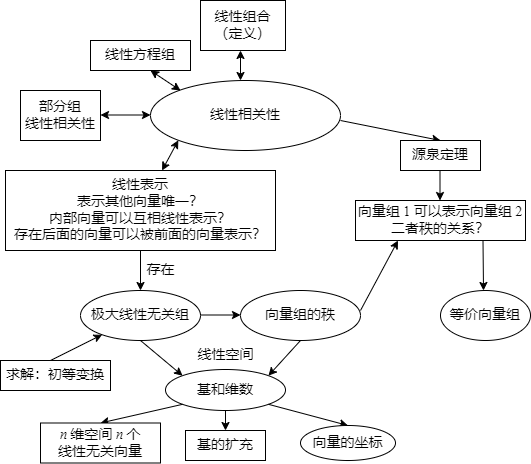
\includegraphics[scale=0.6]{figs/3-1.png}
    \end{figure}

    事实上,与其他内容风格不一样的是,本讲中很大一部分的定理我们都给出了证明,一方面是为了提升阅读体验,防止在初学时就被多个``显然''等词汇困惑,另一方面也是希望读者能够从这些比较规范的证明中得到一些证明的技巧.

    也许读到这里很多读者都会有些迷惑与焦急——为什么我们仿佛在学习很多看起来十分抽象而且似乎没什么实际应用的知识呢?或许我们需要在这里给读者一个``定心丸''. 事实上,我们在上一讲中定义的线性空间运算法则就是从一般向量加法数乘运算法则抽象而来的最为抽象和基本的内容,我们仅仅建立在这一基础上,伴随着线性表示、线性扩张、线性相关等概念的提出,导出了(有限维)线性空间都具有一种统一的本质结构描述——基和维数,由此我们从抽象的运算规则走到了比较具体的结构. 在此基础上,我们基本上将单个线性空间的研究完成,之后我们将会讨论线性空间之间的关系——一方面可以定义线性空间之间的运算,我们将在下一讲详细介绍,另一方面可以建立两个线性空间之间的某种映射,在关于这种映射的讨论中我们会发现线性空间的本质结构是维数,甚至基之间的差异都可以完全被遮蔽(只需通过本讲介绍的坐标即可),然后我们对线性空间的认识便可以从某种比较抽象的结构走向大家熟悉的一定长度的向量,接下来便可以定义更为具象的矩阵. 这一路上我们实际上是从最为抽象的内容逐步定义概念,说明定理,走向具象的内容. 不同于一般线性代数从行列式、矩阵开始,这样的思路一定能让读者对线性代数有更为深刻的认识.

\end{summary}

\begin{exercise}
    \exquote[柯西]{给我五个系数,我将画出一头大象;给我六个系数,大象将会摇动尾巴.}

    \begin{exgroup}
        \item 下列命题是否正确?若正确请证明,否则举出反例.
        \begin{enumerate}
            \item 若 $\alpha_1, \ldots, \alpha_m \ (m > 2)$ 线性相关,则其中每一向量都是其余向量的线性组合;

            \item 若 $\alpha_1, \ldots, \alpha_m$ 线性无关,则其中每一向量不是其余向量的线性组合,这个命题的等价命题应如何叙述?

            \item $\alpha_1, \ldots, \alpha_m \ (m > 2)$ 线性无关的充要条件是任意两个向量都线性无关;

            \item  若 $\alpha_1, \alpha_2$ 线性相关,$ \beta_1, \beta_2$ 线性相关,则 $\alpha_1 + \beta_1, \alpha_2 + \beta_2$ 也线性相关;

            \item 若 $\alpha_1, \ldots, \alpha_n$ 线性无关,则 $\alpha_1 + \alpha_2, \alpha_2 + \alpha_3, \ldots, \alpha_{n-1} + \alpha_n, \alpha_n + \alpha_1$ 也线性无关;

            \item 若 $\alpha_1, \alpha_2, \alpha_3$ 线性相关,则 $\alpha_1 + \alpha_2, \alpha_2 + \alpha_3, \alpha_3 + \alpha_1$ 也线性相关;

            \item 设 $B = \{\alpha_1, \alpha_2, \alpha_3\}$ 是 $ \mathbf{R}^3 $ 的一组基,非零向量 $\alpha_0 \in \mathbf{R}^3$,则 $\{\alpha_0 + \alpha_1, \alpha_0 + \alpha_2, \alpha_0 + \alpha_3\}$ (其中三个向量均是非零向量) 也是 $\mathbf{R}^3$ 的一组基;

            \item  设 $B = \{\alpha_1, \alpha_2\}$ 是 $\mathbf{R}^2$ 的一组基,则 $\{\alpha_1 + \alpha_2, \alpha_1 - \alpha_2\}$ 也是 $\mathbf{R}^2$ 的一组基;

            \item 一个有限维线性空间内只含有有限个子空间;

            \item  若 $W_1, W_2$ 是 $ \mathbf{R}^n $ 的两个子空间,$B_1, B_2$ 分别是 $W_1, W_2$ 的基,则存在 $ \mathbf{R}^n $ 的一组基 $B$,使得 $B \supseteq B_1 \cup B_2$。

        \end{enumerate}
        \begin{answer}
            \begin{enumerate}
                \item 错. 反例:$\alpha_1=(1,0),\alpha_2=(2,0),\alpha_3=(0,1)$,则 $\alpha_1,\alpha_2,\alpha_3$ 线性相关而 $\alpha_3$ 不是 $\alpha_1.\alpha_2$ 的线性组合.

                \item 对. 该命题的等价命题(逆否命题)是:若存在一个向量是其余向量的线性组合,则 $\alpha_1,\ldots,\alpha_m$ 线性相关. 这正是定理 3.1 的内容,因而成立.

                \item 错. 反例:$\alpha_1=(1,0),\alpha_2=(0,1),\alpha_3=(1,1)$,则 $\alpha_1,\alpha_2,\alpha_3$ 两两无关,而三者线性相关. 可证两两无关是向量组无关的必要条件.

                \item 错. 反例:$\alpha_1=(1,0),\alpha_2=(0,0),\beta_1=(0,0),\beta_2=(0,1)$,有 $\alpha_1,\alpha_2$ 相关,$\beta_1,\beta_2$ 相关,而 $\alpha_1+\beta_1$ 与 $\alpha_2+\beta_2$ 线性无关.

                \item 错. 若 $\alpha_1,\ldots,\alpha_n$ 线性无关,有
                    \[\lambda_1\alpha_1+\cdots+\lambda_n\alpha_n\implies\lambda_1=\lambda_2=\cdots=\lambda_n=0,\]
                    判断 $\alpha_1+\alpha_2,\alpha_2+\alpha_3,\ldots,\alpha_n+\alpha_1$ 是否无关. 设
                    \[\lambda_1'(\alpha_1+\alpha_2)+\cdots+\lambda_n'(\alpha_n+\alpha_1)=0,\]
                    则
                    \[(\lambda_n'+\lambda_1')\alpha_1+(\lambda_1'+\lambda_2')\alpha_2+\cdots+(\lambda_{n-1}'+\lambda_{n}')\alpha_n=0,\]
                    则
                    \[\begin{cases} \begin{aligned}
                                \lambda_n'+\lambda_1'       & = 0               \\
                                                            & \vdotswithin{ = } \\
                                \lambda_{n-1}'+\lambda_{n}' & = 0               \\
                            \end{aligned} \end{cases}.\]
                    解该方程可得 $\lambda_n'=(-1)^n\lambda_1'$,因此当 $n$ 为偶数时,上述方程组有非零解,则向量组相关,而当 $n$ 为奇数时,向量组无关. 综上,该命题不成立.

                \item 对. 由定理 3.1,不妨设 $\alpha_3$ 可由 $\alpha_1,\alpha_2$ 线性表示,则 $\alpha_1+\alpha_2,\alpha_2+\alpha_3,\alpha_3+\alpha_1$ 均可由 $\alpha_1,\alpha_2$ 线性表示,再由定理 3.3 可知,$\alpha_1+\alpha_2,\alpha_2+\alpha_3,\alpha_3+\alpha_1$ 线性相关.

                \item 错. 反例:取 $\alpha_0=\alpha_1-\alpha_2-\alpha_3$,则 $\alpha_0+\alpha_1=(\alpha_0+\alpha_2)+(\alpha_0+\alpha_3)$,三者线性相关,不是 $\mathbf{R}^3$ 的基.

                \item 对. 判断 $\alpha_1+\alpha_2$ 与 $\alpha_1-\alpha_2$ 是否无关.
                    \[\lambda_1(\alpha_1+\alpha_2)+\lambda_2(\alpha_1-\alpha_2)=0,\]
                    则有$(\lambda_1+\lambda_2)\alpha_1+(\lambda_1-\lambda_2)\alpha_2=0$,则 $\lambda_1+\lambda_2=0,\lambda_1-\lambda_2=0\implies \lambda_1=\lambda_2=0$,因此线性无关且个数等于维数,是一组基.

                \item 错. 反例:$\mathbf{R}^2$ 中过原点的直线 $L_0$ 是 $\mathbf{R}^2$ 的一个子空间. 显然这样的直线有无数条.

                \item 错. 反例:$\mathbf{R}^3$ 中,子空间 $W_1=\spa(e_1,e_2)$,$W_2=\spa(e_1+e_2,e_3)$,则 $B_1\cup B_2=\{e_1,e_2,e_3,e_1+e_2\}$,显然 $\mathbf{R}^3$ 中的任一组基都不可能包含四个元素.
            \end{enumerate}
        \end{answer}

        \item 证明:如果向量组线性相关,把每个向量去掉$m$个位置一致的分量,得到的缩短组仍线性相关;如果向量组线性无关,把每个向量添加$m$个位置一致的分量,得到的缩短组仍线性无关;
        \begin{answer}
            \begin{enumerate}
                \item 若向量组线性相关,则对应该方程组有无穷多解. 去掉 $m$ 个分量,相当于删去该方程组中的任意 $m$ 行方程,依然有无穷多解. 这是因为对于原方程组的任意一个解,将其带入被削减后的方程组也依然成立. 故线性相关得证.

                \item 若向量组线性无关,对应原方程组仅有唯一解,也就是全零解. 增加 $m$ 个分量相当于增加 $m$ 个方程,依然只有唯一解,因为若出现非零解,代入原方程组对应的方程中不会成立,矛盾. 故线性无关得证.
            \end{enumerate}
        \end{answer}

        \item $a$取何值时,$\beta_1=(1,3,6,2)^\mathrm{T},\beta_2=(2,1,2,-1)^\mathrm{T},\beta_3=(1,-1,a,-2)^\mathrm{T}$线性无关?
        \begin{answer}
            方程组:$x_1\beta_1+x_2\beta_2+x_3\beta_3=0$ 系数矩阵
            \[\begin{pmatrix}
                    1 & 2  & 1  \\
                    3 & 1  & -1 \\
                    6 & 2  & a  \\
                    2 & -1 &
                    -2\end{pmatrix}\rightarrow\begin{pmatrix}
                    1 & 2   & 1   \\
                    0 & -5  & -4  \\
                    0 & -10 & a-6 \\
                    0 & -6  & -4
                \end{pmatrix}\rightarrow\begin{pmatrix}
                    1 & 2  & 1   \\
                    0 & -5 & -4  \\
                    0 & 0  & a+2 \\
                    0 & 0  & 0
                \end{pmatrix},\]
            仅全零解的条件是 $a\neq-2$,此时向量组线性无关.
        \end{answer}

        \item 设$\alpha_1,\alpha_2,\ldots,\alpha_n\in\mathbf{F}^n$. 证明:$\alpha_1,\alpha_2,\ldots,\alpha_n$线性无关的充要条件是$\mathbf{F}^n$中任一向量都可以由它们线性表示.
        \begin{answer}
            \begin{enumerate}
                \item 必要性:$\alpha_1,\ldots,\alpha_n$ 线性无关,对于 $F^n$ 中的任一向量 $\beta$, $\alpha_1,\ldots,\alpha_n,\beta$ 的向量个数大于维数 $n$,则线性相关. 由定理 3.2,$\beta$ 可被 $\alpha_1,\ldots,\alpha_n$ 唯一表示.

                \item 充分性:由于 $F^n$ 中任意向量均可被 $\alpha_1,\ldots,\alpha_n$ 线性表示,并且向量个数等于维数. 则 $\alpha_1,\ldots,\alpha_n$ 是 $F^n$ 的一组基. 则 $\alpha_1,\ldots,\alpha_n$ 线性无关.

                      $^*$ 更详细的证明:对于 $F^n$ 的一组基 $e_1,\ldots,e_n$,其可被 $\alpha_1,\ldots,\alpha_n$ 表示. 若 $\alpha_1,\ldots,\alpha_n$ 线性相关,不妨设 $\alpha_n$ 可被 $\alpha_1,\ldots,\alpha_{n-1}$ 表示,则有 $e_1,\ldots,e_n$ 可被 $\alpha_1,\ldots,\alpha_{n-1}$ 表示. 由于 $e_1,\ldots,e_n$ 线性无关. 根据定理 3.3,$n\leqslant n-1$,矛盾. 因此得证.
            \end{enumerate}
        \end{answer}

        \item 设$S_1=\{\alpha_1,\ldots,\alpha_s\},S_2=\{\beta_1,\ldots,\beta_t\}$是向量空间$V$的两个线性无关的子集,证明:$\alpha_1,\ldots,\alpha_s,\beta_1,\ldots,\beta_t$线性无关$\iff \spa(S_1)\cap \spa(S_2)=\{0\}$.
        \begin{answer}
            \begin{enumerate}
                \item 必要性:对于 $\forall v\in\spa(S_1) \cap \spa(S_2)$ 有 $v=a_1\alpha_1+\cdots+a_s\alpha_s=b_1\beta_1+\cdots+b_t\beta_t$. 由于 $\alpha_1,\ldots,\alpha_s,\beta_1,\ldots,\beta_t$ 线性无关 $\implies a_1=\cdots=a_s=b_1=\cdots=b_t=0$,则 $v=0$,即 $\spa(S_1)\cap\spa(S_2)=\{0\}$.

                \item 充分性:考虑反证法. 如果 $\alpha_1,\ldots,\alpha_s,\beta_1,\ldots,\beta_t$ 线性相关,则存在不全为零的系数使得 $a_1\alpha_1+\cdots+a_s\alpha_s+b_1\beta_1\cdots+b_t\beta_t=0$. 因此存在一个向量 $v=a_1\alpha_1+\cdots+a_s\alpha_s=-(b_1\beta_1\cdots+b_t\beta_t)\neq 0$ 且 $v\in\spa(S_1),v\in\spa(S_2)$. 即存在非零向量 $v$ 属于 $\spa(S_1),v\in\spa(S_2)$,矛盾!则充分性得证.
            \end{enumerate}
        \end{answer}

        \item 完成 \autoref{lem:初等行变换不改变列的线性相关性} 其它两种初等行变换的证明.
        \begin{answer}
            设矩阵为
            \[
                \begin{pmatrix}
                    a_{11} & a_{12} & \cdots & a_{1n} \\
                    a_{21} & a_{22} & \cdots & a_{2n} \\
                    \vdots & \vdots & \ddots & \vdots \\
                    a_{m1} & a_{m2} & \cdots & a_{mn}
                \end{pmatrix},
            \]

            \begin{enumerate}
                \item 对其进行倍乘行变换,即将第 $i$ 行乘以 $c$,那么第 $i$ 行会变为 $c a_{i1}, c a_{i2}, \ldots, c a_{in}$,而其他行不变. 记原先矩阵的列向量为 $S_A = \{\alpha_1,\alpha_2,\ldots,\alpha_n\}$,变换后的矩阵列向量为 $S_B = \{\beta_1,\beta_2,\ldots,\beta_n\}$.

                    先证 $S_A$ 线性相关 $\implies S_B$ 线性相关:若 $S_A$ 线性相关,则存在不全为零的系数 $x_1, x_2, \ldots, x_n$ 使得 $x_1 \alpha_1 + x_2 \alpha_2 + \cdots + x_n \alpha_n = 0$. 由于 $S_B$ 与 $S_A$ 只有第 $i$ 行不同,我们仅需要判断第 $i$ 行中的元素在系数 $x_1, x_2, \ldots, x_n$ 下的线性组合是否为 $0$ 即可. 事实上我们有 $x_1 c a_{i1} + x_2 c a_{i2} + \cdots + x_n c a_{in} = c(x_1 a_{i1} + x_2 a_{i2} + \cdots + x_n a_{in}) = 0$,故 $S_B$ 线性相关.

                    再证 $S_B$ 线性相关 $\implies S_A$ 线性相关:若 $S_B$ 线性相关,由于倍乘行变换保证 $c \neq 0$,故从 $S_B$ 到 $S_A$ 相当于做一次将第 $i$ 行乘以 $\frac{1}{c}$ 的行变换,同理可得 $S_A$ 线性相关.

                    因此,对矩阵做倍乘行变换不改变矩阵的列的线性相关性.

                \item 对其进行对换行变换,即将第 $i$ 行与第 $j$ 行交换,其他行不变. 记原先矩阵的列向量为 $S_A = \{\alpha_1,\alpha_2,\ldots,\alpha_n\}$,变换后的矩阵列向量为 $S_B = \{\beta_1,\beta_2,\ldots,\beta_n\}$.

                    先证 $S_A$ 线性相关 $\implies S_B$ 线性相关:若 $S_A$ 线性相关,则存在不全为零的系数 $x_1, x_2, \ldots, x_n$ 使得 $x_1 \alpha_1 + x_2 \alpha_2 + \cdots + x_n \alpha_n = 0$. 由于 $S_B$ 与 $S_A$ 只有第 $i$ 行与第 $j$ 行不同,我们仅需要判断第 $i$ 行与第 $j$ 行中的元素在系数 $x_1, x_2, \ldots, x_n$ 下的线性组合是否均为 $0$ 即可. 事实上由原先第 $i$($j$)行的元素在 $x_1, x_2, \ldots, x_n$ 下的线性组合为 $0$ 即可得到变换后第 $j$($i$)行的元素的线性组合为 $0$,故 $S_B$ 线性相关.

                    再证 $S_B$ 线性相关 $\implies S_A$ 线性相关:若 $S_B$ 线性相关,从 $S_B$ 到 $S_A$ 相当于再做一次相同的对换行变换,同理有 $S_A$ 线性相关.

                    因此,对矩阵做对换行变换不改变矩阵的列的线性相关性.
            \end{enumerate}
        \end{answer}

        \item 已知$\alpha_1=(1,2,4,3),\alpha_2=(1,-1,-6,6),\alpha_3=(-2,-1,2,-9),\alpha_4=(1,1,-2,7),\beta=(4,2,4,a)$.
        \begin{enumerate}
            \item 求子空间$\spa(\alpha_1,\alpha_2,\alpha_3,\alpha_4)$的维数和一组基;

            \item 求$a$的值使得$\beta\in W$,并求$\beta$在 (1) 所选基下的坐标.
        \end{enumerate}
        \begin{answer}
            \begin{enumerate}
                \item 也就是求 $\alpha_1,\alpha_2,\alpha_3,\alpha_4$ 的极大线性无关组. 利用讲义中所述求法:方程组
                      \[ a_1\alpha_1+\cdots+a_4\alpha_4=0 \]
                      对应系数矩阵 $\begin{pmatrix}
                              1 & 1  & -2 & 1  \\
                              2 & -1 & -1 & 1  \\
                              4 & -6 & 2  & -2 \\
                              3 & 6  & -9 & 7\end{pmatrix}$. 化简为行阶梯型:$\begin{pmatrix}
                              1 & 1  & -2 & 1  \\
                              0 & -3 & 3  & -1 \\
                              0 & 0  & 0  & 3  \\
                              0 & 0  & 0  & 0\end{pmatrix}$,因此 $\alpha_1,\alpha_2,\alpha_3,\alpha_4$ 有非零解,这四个向量线性相关. (其实此处已知矩阵秩为 3,即维数是 3).

                      再选取 $\alpha_1,\alpha_2,\alpha_4$ 来求解方程 $a_1\alpha_1+a_2\alpha_2+a_4\alpha_4=0$:
                      \[\begin{pmatrix}
                              1 & 1  & 1  \\
                              2 & -1 & 1  \\
                              4 & -6 & -2 \\
                              3 & 6  & 7\end{pmatrix}\rightarrow\begin{pmatrix}
                              1 & 1  & 1  \\
                              0 & -3 & -2 \\
                              0 & 0  & 2  \\
                              0 & 0  & 0\end{pmatrix},\]
                      因此该方程组只有全零解,即 $\alpha_1,\alpha_2,\alpha_4$ 是$\alpha_1,\alpha_2,\alpha_3,\alpha_4$的极大线性无关组. 则 $\spa(\alpha_1,\alpha_2,\alpha_4)$ 的维数是 3. 一组基是 $\alpha_1,\alpha_2,\alpha_4$ .

                \item 也就是 $a_1\alpha_1+\cdots+a_4\alpha_4=\beta$有解:增广矩阵 $\begin{pmatrix}
                              1 & 1  & -2 & 1  & 4 \\
                              2 & -1 & -1 & 1  & 2 \\
                              4 & -6 & 2  & -2 & 4 \\
                              3 & 6  & -9 & 7  & a\end{pmatrix}$化为 $\begin{pmatrix}
                              1 & 1  & -2 & 1         & 4   \\
                              0 & -3 & 3  & -1        & -6  \\
                              0 & 0  & 0  & -\frac 83 & 8   \\
                              0 & 0  & 0  & 0         & a-9\end{pmatrix}$,若方程有解,则 $a=9$. 求坐标,取 $x_3=0$ 代入得 $\beta=4\alpha_1+3\alpha_2-3\alpha_4$.
            \end{enumerate}
        \end{answer}

        \item 求解子空间 $V_1 = \{(a,0,b) \mid a,b \in \mathbf{R}\}$ 和 $V_2 = \{(a,2a,b) \mid a,b \in \mathbf{R}\}$ 的基和维数.
        \begin{answer}

        \end{answer}

        \item 证明:$B=\{1,x-a,(x-a)^2\}\enspace(a\neq 0)$是$\mathbf{R}[x]_3$的一组基,并求$\mathbf{R}[x]_3$的自然基$\{1,x,x^2\}$中每个向量关于基$B$的坐标.
        \begin{answer}
            只需证明 $B$ 线性无关即可. $\lambda_1+\lambda_2(x_a)+\lambda_3(x-a)^2$求导,增加方程数得到
            \begin{gather*}
                \lambda_2+2\lambda_3x=0, \\
                2\lambda_3=0,
            \end{gather*}
            则 $\lambda_1=\lambda_2=\lambda_3$,线性无关得证. 又 $B$ 中向量个数等于 $R[x]_3$ 维数. 则 $B$ 是一组基. $1=1 \cdot 1+0 \cdot (x-a)+0\times(x-a)^2$ ,即 $(1,0,0)$;$x=a \cdot 1+1 \cdot (x-a)+0\times(x-a)^2$ ,即 $(a,1,0)$;$x^2=a^2 \cdot 1+2a \cdot (x-a)+1\times(x-a)^2$ ,即 $(a^2,2a,1)$.
        \end{answer}

        \item 已知向量组$A=\{\alpha_1,\alpha_2,\alpha_3\},\enspace B=\{\alpha_1,\alpha_2,\alpha_3,\alpha_4\},\enspace C=\{\alpha_1,\alpha_2,\alpha_3,\alpha_5\}$的秩分别为$r(A)=r(B)=3,\enspace r(C)=4$. 证明:$\{\alpha_1,\alpha_2,\alpha_3,\alpha_5-\alpha_4\}$的秩为4.
        \begin{answer}
            等价于证明 $\alpha_1,\alpha_2,\alpha_3,\alpha_5-\alpha_4$ 线性无关. 即求解
            \begin{equation}
                \lambda_1\alpha_1+\lambda_2\alpha_2+\lambda_3\alpha_3+\lambda_4(\alpha_5-\alpha_4)=0. \tag{*} \label{eq:3:A.10}
            \end{equation}

            由于 $r(A)=r(B)=3$ 可得 $A$ 线性无关. $B$ 线性相关. 由定理 3.2 得 $\alpha_4$ 可由 $\alpha_1,\alpha_2,\alpha_3$ 唯一表示:$\alpha_4=\mu_1\alpha_1+\mu_2\alpha_2+\mu_3\alpha_3$. 则代入 (\ref*{eq:3:A.10}) 式. 有
            \[(\lambda_1-\mu_1\lambda_4)\alpha_1+(\lambda_2-\mu_2\lambda_4)\alpha_2+(\lambda_3-\mu_3\lambda_4)\alpha_3+\lambda_4\alpha_5=0,\]
            因为 $r(C)=4$,$\alpha_1,\alpha_2,\alpha_3,\alpha_5$ 线性无关. 有 $\lambda_4=0,\lambda_1=\mu_1\lambda_4=0,\lambda_2=\mu_2\lambda_4=0,\lambda_3=\mu_3\lambda_4=0$. 故 $\alpha_1,\alpha_2,\alpha_3,\alpha_5-\alpha_4$ 线性无关. 原题得证.
        \end{answer}

        \item 设向量组$\alpha_1,\alpha_2,\ldots,\alpha_s$的秩为$r$. 在其中任取$m$个向量$\alpha_{i1},\alpha_{i2},\ldots,\alpha_{im}$,证明:向量组$\alpha_{i1},\alpha_{i2},\ldots,\alpha_{im}$的秩$\geqslant r+m-s$.
        \begin{answer}
            相当于从 $\alpha_1,\ldots,\alpha_s$ 向量中选取 $s-m$ 个向量丢弃,剩余向量的秩:
            \[r(\alpha_{i1},\ldots,\alpha_{im})\geqslant r-(s-m) =r+m-s.\]
        \end{answer}

        \item 已知$\alpha_1,\alpha_2,\ldots,\alpha_n$线性无关,而$\alpha_1,\alpha_2,\ldots,\alpha_n,\beta,\gamma$线性相关. 证明:要么$\beta,\gamma$可以由$\alpha_1,\alpha_2,\ldots,\alpha_n$线性表示,要么$\alpha_1,\alpha_2,\ldots,\alpha_n,\beta$与$\alpha_1,\alpha_2,\ldots,\alpha_n,\gamma$等价.
        \begin{answer}
            方程:$\lambda_1\alpha_1+\cdots+\lambda_n\alpha_n+\lambda_{n+1}\beta+\lambda_{n+2}\gamma=0$,显然 $\lambda_{n+1},\lambda_{n+2}$ 不全为零. 否则与 $\alpha_1,\ldots,\alpha_n$ 线性无关矛盾.
            \begin{enumerate}
                \item 若 $\lambda_{n+1}=0,\lambda_{n+2}\neq 0$,则 $\gamma$ 可被 $\alpha_1,\ldots,\alpha_n$ 表示. 若 $\lambda_{n+1}\neq0,\lambda_{n+2}=0$, 则 $\beta$ 可被 $\alpha_1,\ldots,\alpha_n$ 表示.

                \item 若 $\lambda_{n+1}\lambda_{n+2}\neq 0$ ,则有
                      \begin{gather*}
                          \beta=-\frac 1{\lambda_{n+1}}(\lambda_1\alpha_1+\cdots+\lambda_n\alpha_n+\lambda_{n+2}\gamma), \\
                          \gamma=-\frac 1{\lambda_{n+2}}(\lambda_1\alpha_1+\cdots+\lambda_n\alpha_n+\lambda_{n+1}\beta).
                      \end{gather*}
                    两组向量可以相互表示. 两者等价. 综上原题得证.
            \end{enumerate}
        \end{answer}
    \end{exgroup}

    \begin{exgroup}
        \item 已知$\alpha_1\neq 0$,则$\alpha_1,\alpha_2,\ldots,\alpha_n$线性相关的充要条件是存在$i\enspace(2 \leqslant i \leqslant n)$使得$\alpha_i$可由$\alpha_1,\alpha_2,\ldots,\alpha_{i-1}$线性表示,且表示法唯一.
        \begin{answer}
            充分性显然成立,下证必要性:由于 $\alpha_1,\ldots,\alpha_n$ 线性相关,则存在 $m$,其能使得 $\alpha_1,\ldots,\alpha_m$ 线性无关的最大下标,有 $1\leqslant m<n$. 因此 $i=m+1$,$\alpha_1,\ldots,\alpha_{i-1}$ 线性无关,$\alpha_1,\ldots,\alpha_i$ 线性相关. 可得 $\alpha_i$ 可被 $\alpha_1,\ldots,\alpha_{i-1}$ 唯一表示.
        \end{answer}

        \item 证明以下两个结论:
        \begin{enumerate}
            \item 设$U$和$W$都是$V$的非零子空间,如果$U\subseteq W$,那么$\dim U \leqslant \dim W$;

            \item 设$U$和$W$都是$V$的非零子空间,$U\subseteq W$,且$\dim U = \dim W$,则$U = W$.
        \end{enumerate}
        \begin{answer}
            \begin{enumerate}
                \item 设 $U$ 的一组基为 $u_1,\ldots,u_m$,$W$ 的一组基为 $w_1,\ldots,w_n$. 由于 $U\subseteq W$,则 $u_1,\ldots,u_m$ 可由 $w_1,\ldots,w_n$ 线性表示,且 $u_1,\ldots,u_m$ 线性无关. 由定理 3.3 的等价命题可得 $m\leqslant n$,则 $m=\dim U\leqslant\dim W=n$ 的得证.

                \item 因为 $\dim U=\dim W$,则 $u_1,\ldots,u_m$ 也是 $W$ 的一组基. 则 $W$ 的任意向量均可由 $u_1,\ldots,u_m$ 表示,可得 $W\subseteq U$,而 $U\subseteq W$,故有 $U=W$ 得证.
            \end{enumerate}
        \end{answer}

        \item 设向量组$\alpha_1,\alpha_2,\ldots,\alpha_n$线性无关. 证明:在向量组$\beta,\alpha_1,\alpha_2,\ldots,\alpha_n$中至多有一个向量$\alpha_i\enspace(1 \leqslant i \leqslant r)$可被其前面的$i$个向量$\beta,\alpha_1,\alpha_2,\ldots,\alpha_{i-1}$线性表示.
        \begin{answer}
            反证法. 若存在两个向量 $\alpha_i,\alpha_j$ 可被前面的向量表示,即
            \begin{gather*}
                \alpha_i=\lambda_0\beta+\lambda_1\alpha_1+\cdots+\lambda_{i-1}\alpha_{i-1}, \\
                \alpha_j=\mu_0\beta+\mu_1\alpha_1+\cdots+\mu_{j-1}\alpha_{j-1}.
            \end{gather*}
            如果 $\lambda_0$ 或者 $\mu_0$ 为 0,则有向量组中的 $\alpha_i$ 或 $\alpha_j$ 可被其他向量线性表示,则该向量组相关,这与条件矛盾. 若 $\lambda_0$ 与 $\mu_0$ 均不为 0,等式可化为
            \begin{gather*}
                \frac 1{\lambda_0}\alpha_i=\beta+\frac{\lambda_1}{\lambda_0}\alpha_1+\cdots+\frac{\lambda_{i-1}}{\lambda_0}\alpha_{i-1}, \\
                \frac 1{\mu_0}\alpha_j=\beta+\frac{\mu_1}{\mu_0}\alpha_1+\cdots+\frac{\mu_{j-1}}{\mu_0}\alpha_{j-1}.
            \end{gather*}
            不妨设 $i>j$. 相减得
            \[\frac 1{\lambda_0}\alpha_i=\left(\frac{\lambda_1}{\lambda_0}-\frac{\mu_1}{\mu_0}\right)\alpha_1+\cdots+\left(\frac{\lambda_i}{\lambda_0}+\frac 1{\mu_0}\right)\alpha_j+\frac{\lambda_{i-1}}{\lambda_0}\alpha_{i-1},\]
            则 $\alpha_i$ 可被其他向量线性表示,因此向量组线性相关,与条件矛盾. 综上,至多有一个向量 $\alpha_i$ 可被前面的相邻线性表示.
        \end{answer}

        \item 证明:$1,e^{\lambda_1\cdot x},e^{\lambda_2\cdot x}$($\lambda_1\neq\lambda_2$且均不为0)线性无关.
        \begin{answer}
            考虑使用求导构造更多方程.
            \[\begin{cases}
                    k_0+k_1\cdot e^{\lambda_1 x}+k_2\cdot e^{\lambda_2 x}=0               \\
                    k_1\lambda_1\cdot e^{\lambda_1 x}+k_2\lambda_2\cdot e^{\lambda_2 x}=0 \\
                    k_1\lambda_1^2\cdot e^{\lambda_1 x}+k_2\lambda_2^2\cdot e^{\lambda_2 x}=0
                \end{cases},\]
          由后两式可知$k_1k_2(\lambda_1-\lambda_0)=0$. 又 $\lambda_1\neq\lambda_2$,故$k_1=k_2=0$,代回第一式得 $k_0=0$,则 $1,e^{\lambda_1x},e^{\lambda_2x}$ 线性无关,得证.
        \end{answer}

        \item 设线性空间$V(\mathbf{F})$中,向量$\beta$是$\alpha_1,\ldots,\alpha_r$的线性组合,但不是$\alpha_1,\ldots,\alpha_{r-1}$的线性组合. 证明:$\spa(\alpha_1,\ldots,\alpha_{r-1},\alpha_r)=\spa(\alpha_1,\ldots,\alpha_{r-1},\beta)$.
        \begin{answer}
            只需证明 $\alpha_r$ 可以被 $\alpha_1,\ldots,\alpha_{r-1},\beta$ 表示即可. 由于 $\beta$ 是 $\alpha_1,\ldots,\alpha_{r-1}$ 的线性组合,若 $\lambda_r=0$,则 $\beta$ 是 $\alpha_1,\ldots,\alpha_{r-1}$ 的线性组合. 这与条件矛盾. 因此 $\alpha_r=-\vspace{1ex}\dfrac 1{\lambda_r}(\lambda_1\alpha_1+\cdots+\lambda_{r-1}\alpha_{r-1}-\beta)$,则这两组向量等价. $\spa(\alpha_1,\ldots,\alpha_{r-1},\alpha_r)=\spa(\alpha_1,\ldots,\alpha_{r-1},\beta)$ 得证.
        \end{answer}

        \item \label{item:3:正实数线性空间}
        设$\mathbf{R}^+$是所有正实数组成的集合,加法和数乘定义如下:
        \[ \forall a,b \in \mathbf{R}_+,\enspace k\in \mathbf{R}\colon\enspace a\oplus b = ab,\enspace k\odot a = a^k \]
        则 $\mathbf{R}^+$关于这一加法和数乘构成一个实线性空间. 求$\mathbf{R}^+$的一组基.
        \begin{answer}
            分析该实线性空间,可以看出加法单位元为 1,数乘单位元为 1. 我们给出一组基:$e$,其中 $e$ 为自然对数的底数. 当然, 2,3 或者 10 都可以作为一组基. 接下来我们验证 $e$ 是 $\mathbf{R}^+$ 的基:$\forall a\in \mathbf{R}^+,\exists k=\ln a\in\mathbf{R}$,满足 $k\odot e=e^k=a$,则 $\spa(e)=\mathbf{R}^+$ 成立. 由于该向量组只有一个元素,且并非设该空间的零元 1,则 $e$ 是线性无关的. 得证.
        \end{answer}
    \end{exgroup}

    \begin{exgroup}
        \item 已知$m$个向量$\alpha_1,\alpha_2,\ldots,\alpha_m$线性相关,但其中任意$m-1$个都线性无关,证明:
        \begin{enumerate}
            \item 若$k_1\alpha_1+\cdots+k_m\alpha_m=0$,则$k_1,\ldots,k_m$全为0或全不为0;

            \item 若以下等式成立
                  \begin{align*}
                      k_1\alpha_1+\cdots+k_m\alpha_m & =0 \\
                      l_1\alpha_1+\cdots+l_m\alpha_m & =0
                  \end{align*}
                  其中$l_1\neq 0$,证明:$\dfrac{k_1}{l_1}=\cdots=\dfrac{k_m}{l_m}$.
        \end{enumerate}
        \begin{answer}
            \begin{enumerate}
                \item 若 不全为 0. 不妨设设至少有 $k_i=0$,则有 $k_1\alpha_1+\cdots+k_{i-1}\alpha_{i-1}+k_{i+1}\alpha_{i+1}+\cdots+k_m\alpha_m=0$,并且系数不全为 0. 因此 $\alpha_1,\ldots,\alpha_{i-1},\alpha_{i+1},\ldots,\alpha_m$ 这 $m-1$ 个向量相关,与题设矛盾. 则原题得证.

                \item $l_1\neq 0$,则 $l_2,\ldots,l_m$ 均不为 0.
                      \begin{enumerate}
                          \item 若 $k_1=\cdots=k_m=0$. 原式显然成立.

                          \item 若 $k_1,\ldots,k_m$ 不全为 0. 则
                                \begin{gather*}
                                    l_1(k_1\alpha_1+\cdots+k_m\alpha_m)=0, \\
                                    k_1(l_1\alpha_1+\cdots+l_m\alpha_m)=0.
                                \end{gather*}
                                两式相减,得
                                \[(k_2l_1-k_1l_2)\alpha_2+\cdots+(k_ml_1-k_1l_m)\alpha_m=0,\]
                                因为 $\alpha_2,\ldots,\alpha_m$ 线性无关. 则以上系数均为 0. 故$\dfrac {k_2}{l_2}=\dfrac {k_1}{l_1},\ldots,\dfrac {k_m}{l_m}=\dfrac {k_1}{l_1}$. 得证.
                      \end{enumerate}
            \end{enumerate}
        \end{answer}

        \item (替换定理)设$\alpha_1,\alpha_2,\ldots,\alpha_r$线性无关,且可以被$\beta_1,\beta_2,\ldots,\beta_n$线性表示,则可以将$\beta_1,\beta_2,\ldots,\beta_n$中的$r$个向量替换成$\alpha_1,\alpha_2,\ldots,\alpha_r$后得到与$\beta_1,\beta_2,\ldots,\beta_n$等价的新向量组(注:可以使用数学归纳法证明).
        \begin{answer}
            利用递推法:当 $r=1$ 时,由于 $\alpha_1$ 线性无关,可得 $\alpha_1\neq 0$. 设 $\alpha_1=\lambda_1\beta_1+\cdots+\lambda_n\beta_n$,则至少存在一个 $\lambda_i\neq 0$,不妨设 $\lambda_1\neq 0$,因此有 $\beta_1=-\vspace{1ex}\dfrac 1{\lambda_1}(-\alpha_1+\lambda_2\beta_2+\cdots+\lambda_n\beta_n)$,故 $\beta_1,\ldots,\beta_n$ 与 $\alpha_1,\beta_2,\ldots,\beta_n$ 等价.

            当 $r=2$ 时,由于 $\alpha_1,\alpha_2$ 无关. 有 $\alpha_1\alpha_2\neq 0$. 根据 $r=1$ 的情况,不妨设 $\beta_1,\ldots,\beta_n$ 与 $\alpha_1,\beta_2,\ldots,\beta_n$ 等价. 因此 $\alpha_2$ 可由 $\alpha_1,\beta_2,\ldots,\beta_n$ 表出:
            \[\alpha_2=\mu_1\alpha_1+\mu_2\beta_2+\cdots+\mu_n\beta_n.\]
            由于 $\alpha_1,\alpha_2$ 无关,故 $\mu_2,\ldots,\mu_n$ 至少有一个非零的数. 不妨设 $\mu_2\neq 0$,同上可得$\alpha_1,\alpha_2,\beta_3,\ldots,\beta_n$ 就与 $\alpha_1,\beta_2,\ldots,\beta_n$ 等价,也与$\beta_1,\beta_2,\ldots,\beta_n$ 等价. 综上,通过递推可知,对正整数 $r$,上述结论依然成立.
        \end{answer}

        \item 设线性空间$V=\mathbf{F}^n$. 证明:
        \begin{enumerate}
            \item 存在$V$的子空间$W$,使得$W$的任一非零向量的分量均不为0;

            \item 若$V$的子空间$W$的任一非零向量的分量均不为0,则$\dim W=1$;

            \item 若$V$的子空间$W$的任一非零向量的零分量个数均不超过$r$,则$\dim W \leqslant r+1$.
        \end{enumerate}
        \begin{answer}
            \begin{enumerate}
                \item $\alpha=(1,1,\ldots,1)^{\mathrm{T}}, W=\spa(\alpha)$,显然 $W$ 是满足条件的一维子空间.

                \item 考虑反证法:若 $\dim W>1$,则 $W$ 中存在线性无关的两向量. 由条件,
                      \[a_1,\ldots,a_n,b_1,\ldots,b_n\neq 0,\]
                      可设 $a_1=kb_1,k\in F$,因此 $\alpha-k\beta=(0,a_2-kb-2,\ldots,a_n-kb_n)^{\mathrm{T}}\in W$. 且由于 $\alpha,\beta$ 无关,$\alpha-k\beta\neq 0$ 但存在分量为 0,这与条件矛盾. 故 $\dim W=1$.

                \item 考虑反证法:若 $\dim W>r+1$,则存在 $r+2$ 个线性无关的向量,设为
                      \begin{align*}
                          \alpha_1     & = (a_{11},a_{12},\ldots,a_{1(r+1)},\ldots,a_{1n})^{\mathrm{T}},                 \\
                                       & \vdotswithin{ = }                                                              \\
                          \alpha_{r+2} & = (a_{(r+2)1},a_{(r+2)2},\ldots,a_{(r+2)(r+1)},\ldots,a_{(r+2)n})^{\mathrm{T}}.
                      \end{align*}
                      取这些向量的前 $r+1$ 个分量组成新的向量组:
                      \begin{align*}
                          \beta_1     & = (a_{11},a_{12},\ldots,a_{1(r+1)})^{\mathrm{T}},             \\
                                      & \vdotswithin{ = }                                            \\
                          \beta_{r+2} & = (a_{(r+2)1},a_{(r+2)2},\ldots,a_{(r+2)(r+1)})^{\mathrm{T}}.
                      \end{align*}
                      由于 $\beta_1,\ldots,\beta_{r+2}$ 是 $r+2$ 个 $r+1$ 维向量,其必然线性相关,则存在不全为 0 的系数 $\lambda_1,\ldots,\lambda_{r+2}$,$\lambda_1\beta_1+\cdots+\lambda_{r+2}\beta_{r+2}=0$.  由于 $\alpha_1,\ldots,\alpha_{r+2}$ 线性无关知:$\lambda_1\alpha_1+\cdots+\lambda_{r+2}\alpha_{r+2}\neq 0$,且其属于 $W$. 但其前 $r+1$ 个分量均为 0,这与条件矛盾. 故 $\dim W\leqslant r+1$ 得证.
            \end{enumerate}
        \end{answer}

        \item 设 $\mathbf{Q}(\sqrt[3]{2}) = \{a+b\sqrt[3]{2}+c\sqrt[3]{4}\mid a,b,c\in\mathbf{Q}\}$,证明 $\mathbf{Q}(\sqrt[3]{2})$ 是 $\mathbf{Q}$ 上的线性空间并求其维数.
        \begin{answer}
            先证明 $\mathbf{Q}(\sqrt[3]{2})$ 是 $\mathbf{Q}$ 上的线性空间:

            $\mathbf{Q}(\sqrt[3]{2})$ 对通常的加法构成交换群以及其封闭性是显然的,在此不再赘述,下阐述数乘性质:
            \begin{enumerate}
                \item $\forall v = a+b\sqrt[3]{2}+c\sqrt[3]{4} \in \mathbf{Q}(\sqrt[3]{2}), \enspace 1 (a+b\sqrt[3]{2}+c\sqrt[3]{4}) = a+b\sqrt[3]{2}+c\sqrt[3]{4}$;

                \item $\forall v = a+b\sqrt[3]{2}+c\sqrt[3]{4} \in \mathbf{Q}(\sqrt[3]{2}), \forall \lambda, \mu \in \mathbf{Q}, \enspace \lambda(\mu v) = (\lambda \mu) v$;

                \item $\forall v = a+b\sqrt[3]{2}+c\sqrt[3]{4} \in \mathbf{Q}(\sqrt[3]{2}), \forall \lambda, \mu \in \mathbf{Q}, \enspace (\lambda + \mu) v = (\lambda + \mu)a + (\lambda + \mu) b\sqrt[3]{2} + (\lambda + \mu) c\sqrt[3]{4} = \lambda(a+b\sqrt[3]{2}+c\sqrt[3]{4}) + \mu(a+b\sqrt[3]{2}+c\sqrt[3]{4}) = \lambda v + \mu v$;

                \item $\forall v = a_1 + b_1\sqrt[3]{2} + c_1\sqrt[3]{4}, u = a_2 + b_2\sqrt[3]{2} + c_2\sqrt[3]{4} \in \mathbf{Q}(\sqrt[3]{2}), \forall \lambda \in \mathbf{Q}, \enspace \lambda(v+u) = \lambda (a_1 + a_2) + \lambda (b_1 + b_2)\sqrt[3]{2} + \lambda (c_1 + c_2)\sqrt[3]{4} = \lambda (a_1 + b_1\sqrt[3]{2} + c_1\sqrt[3]{4}) + \lambda (a_2 + b_2\sqrt[3]{2} + c_2\sqrt[3]{4}) = \lambda v + \lambda u$;

                \item (封闭性)$\forall v = a+b\sqrt[3]{2}+c\sqrt[3]{4} \in \mathbf{Q}(\sqrt[3]{2}), \forall \lambda \in \mathbf{Q}, \enspace \lambda v = \lambda a + \lambda b\sqrt[3]{2} + \lambda c\sqrt[3]{4} \in \mathbf{Q}(\sqrt[3]{2})$.
            \end{enumerate}
            故 $\mathbf{Q}(\sqrt[3]{2})$ 是 $\mathbf{Q}$ 上的线性空间.

            下求 $\mathbf{Q}(\sqrt[3]{2})$ 的维数. 考虑找 $\mathbf{Q}(\sqrt[3]{2})$ 的一组基,我们给出 $\{1, \sqrt[3]{2}, \sqrt[3]{4}\}$,下证其为 $\mathbf{Q}(\sqrt[3]{2})$ 的一组基:

            \begin{enumerate}
                \item (线性无关)令 $k_1 + k_2 \sqrt[3]{2} + k_3 \sqrt[3]{4} = 0$,其中 $k_1, k_2, k_3 \in \mathbf{Q}$,由于左边只有第一项为有理数,故有 $k_1 = 0$,进而有 $\sqrt[3]{2} (k_2 + k_3 \sqrt[3]{2}) = 0$,又可得到 $k_2 = 0$,并且 $k_3 = 0$. 故 $\{1, \sqrt[3]{2}, \sqrt[3]{4}\}$ 线性无关.

                \item (张成空间)由 $\mathbf{Q}(\sqrt[3]{2})$ 的定义易得.
            \end{enumerate}
            综上,$\mathbf{Q}(\sqrt[3]{2})$ 是 $\mathbf{Q}$ 上的线性空间,且 $\dim \mathbf{Q}(\sqrt[3]{2}) = 3$.

        \end{answer}

        \item 设$\mathbf{K} \subseteq \mathbf{F} \subseteq \mathbf{E}$是三个数域,已知$\mathbf{F}$作为$\mathbf{K}$上的线性空间是$n$维的,$\mathbf{E}$作为$\mathbf{F}$上的线性空间是$m$维的,证明:$\mathbf{E}$作为$\mathbf{K}$上的线性空间是$mn$维的.
        \begin{answer}
            取 $\mathbf{F}(\mathbf{K})$ 的一组基 $f_1, f_2, \ldots, f_n$,$\mathbf{E}(\mathbf{F})$ 的一组基 $e_1, e_2, \ldots, e_m$,下证向量组 $B = \{f_1 e_1, f_2 e_1, \ldots, f_n e_1, f_1 e_2, f_2 e_2, \ldots, f_n e_2, \ldots, f_1 e_m, f_2 e_m, \ldots, f_n e_m\}$ 是 $\mathbf{E}(\mathbf{K})$ 的一组基:

            \begin{enumerate}
                \item (线性无关)令 $k_{11} f_1 e_1 + k_{12} f_2 e_1 + \cdots + k_{1n} f_n e_1 + k_{21} f_1 e_2 + k_{22} f_2 e_2 + \cdots + k_{2n} f_n e_2 + \cdots + k_{m1} f_1 e_m + k_{m2} f_2 e_m + \cdots + k_{mn} f_n e_m = 0$,其中 $k_{ij} \in \mathbf{K}$,则
                    \[
                        \sum_{i=1}^m \left(\sum_{j=1}^n k_{ij} f_j \right) e_i = 0.
                    \]
                    由于 $e_1, e_2, \ldots, e_n$ 是 $\mathbf{E}(\mathbf{F})$ 的一组基 $e_1, e_2, \ldots, e_m$,我们有
                    \[
                        \sum_{j=1}^n k_{ij} f_j = 0, \enspace \forall i = 1, 2, \ldots, m.
                    \]
                    而 $f_1, f_2, \ldots, f_n$ 又是 $\mathbf{F}(\mathbf{K})$ 的一组基,故 $k_{ij} = 0$,即向量组 $B$ 线性无关.

                \item (张成空间)$\forall e = \mu_1 e_1 + \mu_2 e_2 + \cdots + \mu_m e_m \in \mathbf{E} \enspace (\mu_1, \mu_2, \ldots, \mu_m \in \mathbf{F})$,由于 $\mu_i \in \mathbf{F}$,故存在 $k_{ij} \in \mathbf{K}$ 使得 $\mu_i = k_{i1} f_1 + k_{i2} f_2 + \cdots + k_{in} f_n$,于是
                    \[
                        e = \sum_{i=1}^m \left(\sum_{j=1}^n k_{ij} f_j \right) e_i
                          = \sum_{i=1}^m \sum_{j=1}^n k_{ij} f_j e_i.
                    \]
                    故 $e \in \spa B$.
            \end{enumerate}
            综上,$B$ 是 $\mathbf{E}(\mathbf{K})$ 的一组基,故 $\dim \mathbf{E}(\mathbf{K}) = mn$.
        \end{answer}

        \item 延续上一讲对于 $\mathbf{F_4}(\mathbf{Z}_2)$ 的讨论,尝试求 $\mathbf{F_4}$ 在 $\mathbf{Z}_2$ 上的一组基及其维数,以及其中每个元素的坐标表示.
        \begin{answer}

        \end{answer}
    \end{exgroup}
\end{exercise}

\chapter{线性空间的运算}

在前述章节中我们对(有限维)线性空间中的基本概念以及研究的基本问题进行了了解. 事实上,很多时候我们还需要研究不同线性空间进行运算后得到的新集合的性质,本节我们将详细展开讨论这一问题.

\section{线性空间的交、并、和}

\begin{definition}{}{}
    设$W_1,W_2$是线性空间$V(\mathbf{F})$的两个子空间,则
    \begin{align*}
        W_1 \cap W_2 & =\{\alpha \mid \alpha\in W_1 \text{~且~} \alpha\in W_2\}            \\
        W_1 \cup W_2 & =\{\alpha \mid \alpha\in W_1 \text{~或~} \alpha\in W_2\}            \\
        W_1 + W_2    & =\{\alpha_1+\alpha_2 \mid \alpha_1\in W_1,\enspace\alpha_2\in W_2\}
    \end{align*}
    分别称为$W_1$和$W_2$的交、并、和.
\end{definition}

交与并的定义实际上与集合交与并的定义类似,而和的定义可能有些许反直觉. 我们可以通过一个例子来体会为什么要定义子空间的和.
\begin{example}{}{子空间运算}
    在$\mathbf{R}^3$中,我们设
    \[\alpha_1=(0,0,1),\ \alpha_2=(0,1,0),\ \alpha_3=(1,0,0).\]
    令$\mathbf{R}^3$子空间$W_1=\spa(\alpha_1,\alpha_2)$,$W_2=\spa(\alpha_1,\alpha_3)$,则$W_1$实际上是$yOz$平面,$W_2$是$xOz$平面,因此我们根据交与并的概念(实际上就是集合取交集和并集)得到$W_1 \cap W_2=\spa(\alpha_1)$(即$z$坐标轴).

    进一步考察并集,事实上显然$W_1 \cup W_2$得到的集合表示$xOz$和$yOz$平面上所有的点. 事实上我们发现,$W_1 \cup W_2$得到的集合关于向量加法、数乘运算并不封闭,例如只需取$\alpha_2+\alpha_3=(0,1,1)$就不在$W_1 \cup W_2$中,因此不再是$\mathbf{R}^3$的子空间.

    接下来我们考察二者之和. 事实上$W_1+W_2=\mathbf{R}^3$. 原因在于
    \begin{enumerate}
        \item $\forall \beta\in W_1 + W_2$,由子空间和的定义可知有$\beta=\beta_1+\beta_2$,其中$\beta_1\in W_1\subseteq \mathbf{R}^3$,$\beta_2\in W_2\subseteq \mathbf{R}^3$,由于$\mathbf{R}^3$是线性空间,其中元素关于加法运算封闭,因此$\beta=\beta_1+\beta_2\in \mathbf{R}^3$,即$W_1+W_2\subseteq \mathbf{R}^3$;

        \item $\mathbf{R}^3$中任一向量$(x,y,z)$总能写成$(x,y,z)=(0,y,z)+(x,0,0)$的形式,其中$(0,y,z)$在$W_1$中,$(x,0,0)$在$W_2$中,因此根据子空间和的定义可知$\mathbf{R}^3\subseteq W_1 + W_2$成立.
    \end{enumerate}
    综上,我们得到$W_1+W_2=\mathbf{R}^3$.
\end{example}

从上面证明$W_1+W_2=\mathbf{R}^3$的过程中我们可以提炼出证明子空间的和等于某一空间的一般方法:本质而言仍然是证明集合相等,因此证明两边包含即可. 证明子空间的和属于某一空间是平凡的,如上述证明的第一部分;第二部分证明某一空间属于子空间和只需要将该空间中任意向量都可分解为各个子空间中向量的和即可.

事实上,根据\autoref{ex:子空间运算} 我们发现,子空间$W_1$和$W_2$的交与和仍然是线性空间,但是它们的并不是线性空间. 事实上,我们可以证明如下定理:
\begin{theorem}{}{}
    设$W_1,W_2$是线性空间$V(\mathbf{F})$的两个子空间,则
    \begin{enumerate}
        \item $W_1 \cap W_2$是$V$的子空间;

        \item $W_1 + W_2$是$V$的子空间;

        \item $W_1 \cup W_2$为$V$的子空间$\iff W_1 \subseteq W_2$或$W_2 \subseteq W_1 \iff W_1 \cup W_2=W_1+W_2$.
    \end{enumerate}
\end{theorem}

定理前两条的证明见教材74页,第三条我们留作习题供读者练习,因为在考试中有出现过. 前两条还可以进行推广,即$V$的有限个子空间的交与和仍然是$V$的子空间.

除此之外,这一定理也告诉我们为什么需要研究子空间的和而更少研究子空间的并:因为子空间的和仍然是线性空间. 直观理解实际上就是和的定义中出现了两个子空间的向量的加法,而构成子空间的核心就是运算封闭,因此这一定义为子空间的和仍构成子空间提供了保证,因此这一定义也是十分自然的.

下面我们来看一个例子,在例子中我们将给出求子空间的和与交的一般方法:
\begin{example}{}{}
    设 $\alpha_1 = (1, 0, -1, 0)$,$\alpha_2 = (0, 1, 2, 1)$,$\alpha_3 = (2, 1, 0, 1)$,是四维实行向量空间 $V$ 中的向量,他们张成的子空间为 $V_1$;又设向量 $\beta_1 = (-1, 1, 1, 1)$,$\beta_2 = (1, -1, -3, -1)$,$\beta_3 = (-1, 1, -1, 1)$ 张成的子空间为 $V_2$,求 $V_1$ 和 $V_2$ 的交与和的基.
\end{example}

\begin{solution}
    \begin{enumerate}
        \item 方法一.  $V_1 +V_2$ 是由 $\alpha_i$ 和 $\beta_i$ 生成的,因此只需要求出这 $6$ 个向量的极大线性无关组即可. 将这 $6$ 个向量按列分块方式拼成矩阵,并用初等行变换将其化为阶梯形矩阵:
              \begin{align*}
                  \begin{pmatrix}
                      1  & 0 & 2 & -1 & 1  & -1 \\
                      0  & 1 & 1 & 1  & -1 & 1  \\
                      -1 & 2 & 0 & 1  & -3 & -1 \\
                      0  & 1 & 1 & 1  & -1 & 1
                  \end{pmatrix}
                  \xrightarrow{}
                  \begin{pmatrix}
                      1 & 0 & 2 & -1 & 1  & -1 \\
                      0 & 1 & 1 & 1  & -1 & 1  \\
                      0 & 2 & 2 & 0  & -2 & -2 \\
                      0 & 0 & 0 & 0  & 0  & 0
                  \end{pmatrix} \\
                  \xrightarrow{}
                  \begin{pmatrix}
                      1 & 0 & 2 & -1 & 1  & -1 \\
                      0 & 1 & 1 & 1  & -1 & 1  \\
                      0 & 0 & 0 & -2 & 0  & -4 \\
                      0 & 0 & 0 & 0  & 0  & 0
                  \end{pmatrix}
              \end{align*}

              所以就可以取 $\alpha_1$,$\alpha_2$,$\beta_1$ 为 $V_1 + V_2$ 的基(不唯一).

              下面再来取 $V_1\cap V_2$ 的基,首先注意到 $\alpha_1$,$\alpha_2$ 是 $V_1$ 的基(从上面的矩阵即可看出),又不难验证 $\beta_1$,$\beta_2$ 是 $V_2$ 的基,$V_2$ 中的向量可以表示为 $\beta_1$,$\beta_2$ 的线性组合. 假设 $t_1\beta_1 + t_2\beta_2$ 属于 $V_1$,则向量组 $\alpha_1, \alpha_2, t_1\beta_1 + t_2\beta_2$ 和向量组 $\alpha_1, \alpha_2$ 的秩相等(因为 $\alpha_1, \alpha_2$ 是 $V_1$ 的基). 因此,我们可以用矩阵方法来求出参数 $t_1, t_2$. 注意到
              \[ \begin{pmatrix}
                      1  & 0 & -t + t_2   \\
                      0  & 1 & t_1 - t_2  \\
                      -1 & 2 & t_1 - 3t_2 \\
                      0  & 1 & -t_1 - t_2
                  \end{pmatrix} \xrightarrow{} \begin{pmatrix}
                      1 & 0 & -t + t_2  \\
                      0 & 1 & t_1 - t_2 \\
                      0 & 2 & -2t_2     \\
                      0 & 0 & 0
                  \end{pmatrix} \xrightarrow{} \begin{pmatrix}
                      1 & 0 & -t + t_2  \\
                      0 & 1 & t_1 - t_2 \\
                      0 & 0 & -2t_1     \\
                      0 & 0 & 0
                  \end{pmatrix} \]

              所以可以得出当且仅当 $t_1 = 0$ 时 $t_1\beta_1 + t_2\beta_2$ 属于 $V_1$,所以 $V_1 \cap V_2$ 的基可取为 $\beta_2$.

        \item 方法二. 求 $V_1 + V_2$ 的基同方法一,现用解线性方程组的方法来求 $V_1 \cap V_2$ 的基. 因为 $\alpha_1$,$\alpha_2$ 是 $V_1$ 的基,$\beta_1$,$\beta_2$ 是 $V_2$ 的基,故对任一向量 $\gamma \in V_1 \cap V_2$,$\gamma = x_1\alpha_1 + x_2\alpha_2 = -x_3\beta_1 - x_4\beta_2$. 因此,求向量 $\gamma$ 等价于求解线性方程组

              \[ x_1\alpha_1 + x_2\alpha_2 + x_3\beta_1 + x_4\beta_2 = 0. \]

              上述线性方程的通解是 $(x_1, x_2, x_3, x_4) = k(-1, 1, 0, 1)$,从而 $\gamma = -k(\alpha_1 - \alpha_2) = -k\beta_2 (k \in \mathbf{R})$,于是 $\beta_2$ 是 $V_1 \cap V_2$ 的基.
    \end{enumerate}
\end{solution}

我们不难发现,两个线性空间的和的求法就是将两个空间的基合并后求极大线性无关组,而交的求法则更具技巧性. 当然这里使用的是简单的向量空间的例子,如果是一般的线性空间,则可以先转化为基下的坐标然后使用上面的方法求解.

\section{覆盖定理}

\begin{theorem}{覆盖定理}{覆盖定理} \index{fugaidingli@覆盖定理}
    设$V_1,V_2,\ldots,V_s$是线性空间$V$的$s$个非平凡子空间,证明:$V$中至少存在一个向量不属于$V_1,V_2,\ldots,V_s$中的任何一个,即$V_1 \cup V_2 \cup \cdots \cup V_s\subsetneq V$.
\end{theorem}

覆盖定理表明任何一个线性空间都不能被自身有限个非平凡子空间通过并得到. 初看可能有些不够自然,但我们可以从简单的几何意义获得直观的理解:有限条直线的并不可能是一个平面. 下面我们利用数学归纳法进行证明.

\begin{proof}
    \begin{enumerate}
        \item 当$s=2$时,由于$V_1,V_2$是非平凡子空间,因此$V$中存在$\alpha\notin V_1$. 若$\alpha\notin V_2$,则结论已经成立. 若$\alpha\in V_2$,由$V_2$非平凡知存在$\beta\notin V_2$. 我们考虑$\alpha+\beta$和$2\alpha+\beta$,则必有这两个向量都不属于$V_2$(否则有$\beta\in V_2$),并且这两个向量也不能同时属于$V_1$(否则两个向量相减等于$\alpha$也属于$V_1$,矛盾). 这就说明这两个向量中至少有一个既不在$V_1$中也不在$V_2$中,因此结论成立.

        \item 对于$s>2$,假设命题对$s-1$个子空间成立,即$V$中存在向量$\alpha\notin V_1\cup V_2\cup\cdots\cup V_{s-1}$. 若$\alpha\notin V_s$,则结论成立. 若$\alpha\in V_s$,由$V_s$非平凡知存在$\beta\notin V_s$. 我们考虑$\alpha+\beta,2\alpha+\beta,\ldots,s\alpha+\beta$,则与归纳基础中同样的原因,必有这$s$个向量都不属于$V_s$,且这$s$个向量中不可能存在两个向量同属于一个$V_i\enspace(i=1,2,\ldots,s-1)$,因此这$s$个向量中至少有一个不在$V_1\cup V_2\cup\cdots\cup V_s$中,因此结论成立.
    \end{enumerate}
\end{proof}

本质而言$s>2$的情况就是将$s-1$个子空间的并视为一个整体,然后套用$s=2$的情况证明. 若将这一定理的条件限制在$V$为有限维线性空间,我们也可以利用Vandermonde行列式的方法证明,详见\autoref{ex:行列式证明覆盖定理}. 事实上覆盖定理在习题中也有出现,例如教材91--92页第8、9题,都是覆盖定理的直接证明. 我们下面再给出一个例子供读者应用覆盖定理:
\begin{example}{}{}
    $V_1,V_2,\ldots,V_s$是线性空间$V$的$s$个非平凡子空间,证明:存在$V$的一组基$\alpha_1,\alpha_2,\ldots,\alpha_n$都不在$V_1,V_2,\ldots,V_s$中.
\end{example}

\begin{proof}
    由\nameref{thm:覆盖定理},$V$中存在向量$\alpha_1\notin V_1\cup V_2\cup\cdots\cup V_s$. 继续取$\alpha_2\notin V_1\cup V_2\cup\cdots\cup V_s\cup\spa(\alpha_1)$,则一定有$\alpha_1,\alpha_2$线性无关. 继续取$\alpha_3\notin V_1\cup V_2\cup\cdots\cup V_s\cup\spa(\alpha_1,\alpha_2)$,则一定有$\alpha_1,\alpha_2,\alpha_3$线性无关. 以此类推,最终得到一组基$\alpha_1,\alpha_2,\ldots,\alpha_n$都不在$V_1,V_2,\ldots,V_s$中.
\end{proof}

\section{维数公式}

\begin{theorem}{线性空间维数公式}{线性空间维数公式}
    设$W_1,W_2$是线性空间$V(\mathbf{F})$的两个子空间,则
    \[\dim W_1+\dim W_2=\dim(W_1+W_2)+\dim(W_1\cap W_2).\]
\end{theorem}
上式称为子空间的维数公式,区别于下一专题中的线性映射基本定理的维数公式. 这一定理的证明思想非常重要,因此此处我们给出证明.

\begin{proof}
    设$\dim W_1=s,\enspace \dim W_2=t,\enspace \dim(W_1\cap W_2)=r$. 设$W_1\cap W_2$的一组基为$\alpha_1,\alpha_2,\ldots,\alpha_r$,则可以扩充为$W_1$的一组基,记为$\alpha_1,\alpha_2,\ldots,\alpha_r,\beta_1,\ldots,\beta_{s-r}$;也可以扩充为$W_2$的一组基,记为$\alpha_1,\alpha_2,\ldots,\alpha_r,\gamma_1,\ldots,\gamma_{t-r}$. 则我们有
    \[W_1+W_2=\spa(\alpha_1,\ldots,\alpha_r,\beta_1,\ldots,\beta_{s-r},\gamma_1,\ldots,\gamma_{t-r})\]
    (如果对这一步有疑问可以回顾\autoref{ex:子空间运算} 中的证明). 由此,我们要证$\dim (W_1+W_2)=s+t-r$,只需证$\alpha_1,\ldots,\alpha_r,\beta_1,\ldots,\beta_{s-r},\gamma_1,\ldots,\gamma_{t-r}$线性无关. 为此,我们设
    \begin{equation}\label{eq:4:维数公式证明1}
        a_1\alpha_1+\cdots+a_r\alpha_r+b_1\beta_1+\cdots+b_{s-r}\beta_{s-r}+c_1\gamma_1+\cdots+c_{t-r}\gamma_{t-r}=0,
    \end{equation}
    即
    \begin{equation}\label{eq:4:维数公式证明2}
        a_1\alpha_1+\cdots+a_r\alpha_r+b_1\beta_1+\cdots+b_{s-r}\beta_{s-r}=-c_1\gamma_1-\cdots-c_{t-r}\gamma_{t-r}.
    \end{equation}
    显然,\autoref{eq:4:维数公式证明2} 等号两端的向量分别属于$W_1$和$W_2$,因此它们都属于$W_1\cap W_2$,因此都可以被$W_1\cap W_2$的基线性表示,即
    \[-c_1\gamma_1-\cdots-c_{t-r}\gamma_{t-r}=d_1\alpha_1+\cdots+d_r\alpha_r,\]
    即
    \begin{equation}\label{eq:4:维数公式证明3}
        c_1\gamma_1+\cdots+c_{t-r}\gamma_{t-r}+d_1\alpha_1+\cdots+d_r\alpha_r=0.
    \end{equation}
    由于$\alpha_1,\ldots,\alpha_r,\gamma_1,\ldots,\gamma_{t-r}$是$W_2$的基,因此\autoref{eq:4:维数公式证明3} 所有系数都为0,即$c_1=\cdots=c_{t-r}=d_1=\cdots=d_r=0$. 代入\autoref{eq:4:维数公式证明2} 后,由于$\alpha_1,\ldots,\alpha_r,\beta_1,\ldots,\beta_{s-r}$是$W_1$的基,因此可得$a_1=\cdots=a_r=b_1=\cdots=b_{s-r}=0$,因此,代入\autoref{eq:4:维数公式证明1} 后可知$\alpha_1,\ldots,\alpha_r,\beta_1,\ldots,\beta_{s-r},\gamma_1,\ldots,\gamma_{t-r}$必定线性无关(因为根据前述证明所有系数只能为0),故得证.
\end{proof}

总结而言,这一定理证明用到的思想就是``设小扩大''. 我们设出最小空间$V_1\cap V_2$的基,然后分别扩充为$V_1$和$V_2$的基,然后观察要证明的等式和已知的联系,然后利用\autoref{eq:4:维数公式证明2} 构造等式两边属于不同空间的向量这一技巧即可. 下面是一个证明思想类似的例子,需要用到矩阵的相关知识,暂未学到的同学可以先略过本题:
\begin{example}{}{}
    已知$A,B$分别是数域$\mathbf{F}$上的$l \times k$和$k \times n$矩阵,$X$是$n \times 1$的列向量. 证明:所有满足$ABX=0$的$BX$构成一个线性空间$V$,且$\dim V = r(B) - r(AB)$.
\end{example}

\begin{proof}
    $V$是线性空间只需要说明其中元素关于加法数乘封闭即可,因为这样$V$就是$\mathbf{F}^k$的子空间. 这一证明非常基本,我们在此略过.

    记$V_1=\{X\mid BX=0\},\enspace V_2=\{X\mid ABX=0\}$,则$V_1\subseteq V_2$,因为$\forall X\in V_1$,有$BX=0$,因此$ABX=A0=0$,即$X\in V_2$,因此$V_1\subseteq V_2$. 利用``设小扩大''的思想,取$V_1$的一组基$\alpha_1,\ldots,\alpha_r$,则可以扩充为$V_2$的一组基,记为$\alpha_1,\ldots,\alpha_r,\alpha_{r+1},\ldots,\alpha_m$,则$r=n-r(B)$,$s=n-r(AB)$,于是
    \begin{align*}
        V & =\{BX\mid ABX=0\}                                                \\
          & =\spa(B\alpha_1,\ldots,B\alpha_r,B\alpha_{r+1},\ldots,B\alpha_m) \\
          & =\spa(B\alpha_{r+1},\ldots,B\alpha_m).
    \end{align*}
    下面证明$B\alpha_{r+1},\ldots,B\alpha_m$线性无关. 为此,设
    \[c_{r+1}B\alpha_{r+1}+\cdots+c_mB\alpha_m=0,\]
    则
    \[B(c_{r+1}\alpha_{r+1}+\cdots+c_m\alpha_m)=0,\]
    因此$c_{r+1}\alpha_{r+1}+\cdots+c_m\alpha_m\in V_1$,因此存在$c_1,\ldots,c_r$使得
    \[c_{r+1}\alpha_{r+1}+\cdots+c_m\alpha_n=c_1\alpha_1+\cdots+c_r\alpha_r,\]
    即
    \[c_{r+1}\alpha_{r+1}+\cdots+c_m\alpha_m-c_1\alpha_1-\cdots-c_r\alpha_r=0.\]
    由于$\alpha_1,\ldots,\alpha_m$线性无关,因此
    \[c_{r+1}=\cdots=c_m=c_1=c_2=\cdots=c_r=0,\]
    因此$B\alpha_{r+1},\ldots,B\alpha_m$线性无关,因此$V$的维数为$s-r=(n-r(AB))-(n-r(B))=r(B)-r(AB)$,得证.
\end{proof}

\section{线性空间的直和}

我们将来证明或者利用和空间时,很多时候都是利用和空间定义进行向量分解. 我们特别重视分解唯一时的情形,因为这对我们的研究很有帮助,这时的和即为直和. 严谨而言,我们有如下定义:
\begin{definition}{}{}
    设$W_1,W_2$是线性空间$V(\mathbf{F})$的两个子空间. 若$W_1 \cap W_2=\{0\}$,则$W_1+W_2$叫做$W_1$与$W_2$的\term{直和}\index{zhihe@直和 (direct sum)},记作$W_1\oplus W_2$.

    进一步地,若$V=W_1\oplus W_2$,则称$W_1,W_2$为\term{互补子空间}\index{xianxingkongjian!hubu@互补子空间 (complementary subspaces)},或$W_1$是$W_2$的补空间,或$W_2$是$W_1$的补空间.
\end{definition}

直和有以下等价的命题,我们证明或者利用直和都可以任意选择:
\begin{theorem}{}{直和等价命题}
    对于子空间$W_1,W_2$,下列命题等价:
    \begin{enumerate}
        \item $W_1+W_2$是直和,即$W_1 \cap W_2=\{0\}$;

        \item $W_1+W_2$中的每个向量$\alpha$的分解式$\alpha=\alpha_1+\alpha_2\enspace(\alpha_1\in W_1,\enspace\alpha_2\in W_2)$唯一;

        \item 零向量的分解式$\vec{0}=\alpha_1+\alpha_2 \enspace(\alpha_1\in W_1,\enspace\alpha_2\in W_2)$仅当$\alpha_1=\alpha_2=\vec{0}$时成立;

        \item $\dim (W_1+W_2)=\dim W_1+\dim W_2$.
    \end{enumerate}
\end{theorem}

定理的证明是基本的,可以参考教材76页. 在实际运用中我们要非常熟悉这些等价条件,因为都可能使用到.

我们也可以定义有限个子空间的直和,即$V=W_1\oplus W_2\oplus\cdots\oplus W_n \iff W_i \cap \sum\limits_{j \neq i}W_j=\{0\}$,即每个子空间与其余子空间的和的交都是$\{0\}$. 等价命题也是上述定理的推广,例如唯一分解、$\vec{0}$的分解以及维数公式推广,此处不再赘述,详见教材76页. 除此之外,我们还有一个与多空间直和相关的定理:
\begin{theorem}{}{多空间直和}
    若$V=V_1\oplus V_2,\enspace V_1=V_{11}\oplus\cdots\oplus V_{1s},\enspace V_2=V_{21}\oplus\cdots\oplus V_{2t}$,则
    \[V=V_{11}\oplus\cdots\oplus V_{1s}\oplus V_{21}\oplus\cdots\oplus V_{2t}\]
\end{theorem}
这一定理的证明是很简单的,实际上利用零向量分解唯一即可.

在习题中我们证明直和一般有两种思路,一种是先证和,再证直和,我们来看一个例子(没有学到矩阵的可以先略过):
\begin{example}{}{}
    数域$\mathbf{F}$上所有$n$阶方阵组成的线性空间$V=\mathbf{M}_n(\mathbf{F})$,$V_1$表示所有对称矩阵组成的集合,$V_2$表示所有反对称矩阵组成的集合. 证明:$V_1,V_2$都是$V$的子空间,且$V=V_1\oplus V_2$.
\end{example}

\begin{proof}
    首先证明和. 事实上,对于任意矩阵$A\in V$,有
    \[A=B+C,\enspace B=\frac{1}{2}(A+A^T),\enspace C=\frac{1}{2}(A-A^T),\]
    其中$B$是对称矩阵,$C$是反对称矩阵,即$B\in V_1$,$C\in V_2$,因此$V_1+V_2=V$(因为$V$中任意元素都可以写成$V_1$和$V_2$元素和的形式,根据和的定义可知成立).

    下面证明直和. 我们有如下三种方法:
    \begin{enumerate}
        \item 利用零向量分解唯一:设$O$是$n$阶零矩阵,设$O=B+C$,其中$B$是对称矩阵,$C$是反对称矩阵. 由于$B$是对称矩阵,因此$B^T=B$,由于$C$是反对称矩阵,因此$C^T=-C$,因此
              \[O=O^T=(B+C)^T=B^T+C^T=B-C\]
              解得$B=C=O$,因此零向量分解唯一,故直和得证;

        \item 利用$V_1\cap V_2=\{0\}$:设$A\in V_1\cap V_2$,则$A=A^T=-A$,因此$A=-A$,即$A=O$,因此$V_1\cap V_2=\{0\}$,故直和得证;

        \item 利用$\dim V_1+\dim V_2=\dim V$:这一方法较为复杂,我们简单阐述思想. 设$E_{ij}$是第$i$行第$j$列元素为1,其余元素为0的矩阵,则$V$的一组基为$E_{ij},\enspace i,j=1,2,\ldots,n$,$V_1$的一组基为$E_{ij}+E_{ji},\enspace i<j$和$E_{ii},\enspace i=1,2,\ldots,n$,$V_2$的一组基为$E_{ij}-E_{ji},\enspace i<j$,则$\dim V_1=\dfrac{n(n-1)}{2},\enspace \dim V_2=\dfrac{n(n-1)}{2}$,因此$\dim V_1+\dim V_2=n^2$,因此$\dim V_1+\dim V_2=\dim V$,故直和得证.
    \end{enumerate}
\end{proof}

还有一种证明$V=V_1\oplus V_2$的方式是先令$W=V_1+V_2$,先证明和为直和(即交为$\{0\}$)再证$W=V$即可,下面是一个例子:
\begin{example}{}{}
    设$A$是数域$\mathbf{F}$上的一个$n$阶可逆方阵,$A$的前$r$个行向量组成的矩阵为$B$,后$n-r$个行向量组成的矩阵为$C$,$n$元线性方程组$BX=0$与$CX=0$的解空间分别为$V_1,V_2$. 证明:$\mathbf{F}^n=V_1\oplus V_2$.
\end{example}

\begin{proof}
    先记$W=V_1+V_2$,若$\alpha\in V_1\cap V_2$,则$B\alpha=C\alpha=0$,所以
    \[A\alpha=\begin{pmatrix}
            B \\
            C
        \end{pmatrix}\alpha=0,\]
    由于$A$可逆,因此$\alpha=0$,即$V_1\cap V_2=\{0\}$,因此$V_1+V_2$是直和,因此只需证$W=\mathbf{F}^n$即可. 事实上,我们知道$r(B)=r,r(C)=n-r$,因此$\dim V_1=n-r,\enspace \dim V_2=n-(n-r)=r$,所以
    \[\dim W=\dim V_1+\dim V_2=n-r+r=n=\dim \mathbf{F}^n,\]
    又$W=V_1\oplus V_2\subseteq \mathbf{F}^n$,因此$W=\mathbf{F}^n$,故得证.
\end{proof}

最后我们要提醒读者注意的是,有限维线性空间的一个子空间的补空间并不唯一,如下面的例子:
\begin{example}{}{}
    在$\mathbf{R}^3$中,$W_1=\spa(\alpha_1)$,则其补空间根据直和的维数公式可知为2,记为$W_2=\spa(\alpha_2,\alpha_3)$. 实际上只需要$\alpha_1,\alpha_2,\alpha_3$线性无关即可,事实上这样的选择是有无穷种的,因为$W_1$本质表示一条直线,故$W_2$是不包含$W_1$且不与$W_1$平行的平面即可,这样$\alpha_2,\alpha_3$是$W_2$任意一组基都可以.
\end{example}

\section{商空间}

这一节我们需要引入代数中一个非常重要的运算,即某个代数结构的商. 在第一讲中我们给出了一个非常重要的概念——等价类,这里的目标是在一个线性空间 $V$ 中定义出等价关系,即利用\autoref{thm:等价类的性质},以某种方式将一个线性空间中的所有向量划分为几个不相交的等价类的并集,最后在此基础上定义出线性空间的商运算.

\subsection{从等价关系出发}

为了定义出这个等价关系,我们首先需要确定的是它应当满足怎样的性质,否则对于如何定义这一等价关系我们将毫无头绪. 这一问题的出发点事实上就隐藏在\autoref{ex:有限域} 后关于``相容''的讨论中. 在那里,我们要求从一般整数加法和乘法继承下来的模$n$剩余类上的加法和乘法是良定义的,类比于这里的目标,则是希望线性空间中等价类的集合上(也就是商集)定义的加法和数乘运算,可以自然地继承一般的向量加法和乘法,并且保证相容性.

下面我们开始形式化地把上面抽象的描述转化为表达式. 我们需要在线性空间$V$中定义一个等价关系$R$,得到一个等价类构成的商集:
\[V/R=\{\overline{v_1},\overline{v_2},\ldots,\overline{v_n},\ldots\},\]
其中$\overline{v_i}$表示$v_i\in V$所在的等价类,取$v_i$为代表元. 需要注意的是,这里的等价类不一定是有限个,因此最后还是省略号.

接下来我们需要定义等价类之间的运算,我们希望自然继承线性空间的加法和数乘运算,故我们定义商集上的加法和数乘运算满足对于任意的$\overline{v_1},\overline{v_2}\in V/R$和$\lambda\in\mathbf{F}$,有
\begin{equation} \label{eq:10:商集运算}
    \begin{gathered}
        \overline{v_1}+\overline{v_2}=\overline{v_1+v_2},\\
        \lambda\overline{v_1}=\overline{\lambda v_1}.
    \end{gathered}
\end{equation}
需要注意的是,等号左边的运算是商集$V/R$上的,右边是线性空间$V$上的,这里不再像模$n$剩余类上的运算定义那样使用不同的符号(例如加法改成$\oplus$)是出于习惯,以及相信读者学习到今天应当适应了为记号上方便做出的牺牲(比如对于任何线性空间,即使加法不是定义成最一般的加法,但也写成加号的形式).

最后我们需要上面的运算保证相容性,也就是说,对于任意的$v_1,v_2,u_1,u_2\in V$,如果$v_1Rv_2$,$u_1Ru_2$则$(v_1+u_1)R(v_2+u_2)$,$\lambda v_1R\lambda v_2$,展开写为:
\begin{gather*}
    \overline{v_1+u_1}=\overline{v_2+u_2},\\
    \overline{\lambda v_1}=\overline{\lambda v_2}.
\end{gather*}

推进到这里或许我们还是很难看出如何定义这一等价关系,但我们可以从简单的角度入手,逐步观察这些等价类的特点. 我们可以首先考虑线性空间的零向量所在的等价类具有什么性质. 事实上,我们很容易得到如下定理:
\begin{theorem}{}{}
    线性空间$V$的零向量所在的等价类$\overline{0}$一定是$V$的子空间.
\end{theorem}
\begin{proof}
    \begin{enumerate}
        \item 加法封闭:$\forall \alpha,\beta\in\overline{0}$,则$\alpha\,R\,0$,$\beta\,R\,0$,因此根据相容性,$\alpha+\beta\,R\,0$,即$\alpha+\beta\in\overline{0}$;
        \item 数乘封闭:$\forall \alpha\in\overline{0}$,则$\alpha\,R\,0$,$\lambda\in\mathbf{F}$,因此根据相容性,$\lambda\alpha\,R\,0$,即$\lambda\alpha\in\overline{0}$.
    \end{enumerate}
\end{proof}

这一结论非常关键,它使得我们把抽象的等价关系与一个子空间绑定. 我们记这一子空间为$U$,即$\overline{0}=U$,于是下面这一结论也是容易得到的:
\begin{theorem}{}{}
    设$v_1,v_2\in V$,则$v_1Rv_2$当且仅当$v_1-v_2\in U$.
\end{theorem}
\begin{proof}
    \begin{enumerate}
        \item ($\implies$) 直接取$u_1,u_2\in U$,即$u_1\,R\,0$,$u_2\,R\,0$,因此根据相容性,$\overline{v_1}+\overline{u_1}=\overline{v_2}+\overline{u_2}$,移项得$\overline{v_1}-\overline{v_2}=\overline{u_2}-\overline{u_1}$,注意到$\overline{v_1}-\overline{v_2}=\overline{v_1}+(-1)\cdot\overline{v_2}=\overline{v_1}+\overline{-v_2}=\overline{v_1-v_2}$,同理有$\overline{u_2}-\overline{u_1}=\overline{u_2-u_1}$,因此$\overline{v_1-v_2}=\overline{u_2-u_1}=\overline{0}$,即$v_1-v_2\in U$;
        \item 设$v_1-v_2=u\in U$,则$\overline{v_1}=\overline{v_2}+\overline{u}=\overline{v_2}+\overline{0}=\overline{v_2}$,因此$v_1Rv_2$.
    \end{enumerate}
\end{proof}

至此,我们完成了对线性空间$V$上的符合相容性的等价关系$R$的性质的讨论. 我们发现,尽管运算定义和相容性的要求非常抽象,但是在线性空间的背景下,我们成功地将$R$与一个子空间$U$对应起来,这个子空间实际上就是等价类$\overline{0}$. 反过来,当我们需要定义线性空间的等价类的时候,我们可以从一个子空间$U$出发,然后定义等价关系$R$为
\begin{equation} \label{eq:10:线性空间等价关系}
    \forall\alpha,\beta\in V,\enspace\alpha\,R\,\beta\iff \alpha-\beta\in U.
\end{equation}
事实上,验证这一关系的确是等价关系是非常简单的:
\begin{enumerate}
    \item (自反性) $\forall \alpha\in V,\enspace\alpha-\alpha=0\in U$,故$\alpha\,R\,\alpha$;

    \item (对称性) $\forall \alpha,\beta\in V,\enspace\alpha\,R\,\beta\implies \alpha-\beta\in U\implies \beta-\alpha=-(\alpha-\beta)\in U\implies \beta\,R\,\alpha$;

    \item (传递性) $\forall \alpha,\beta,\gamma\in V,\enspace\alpha\,R\,\beta,\enspace\beta\,R\,\gamma\implies \alpha-\beta\in U,\enspace\beta-\gamma\in U\implies \alpha-\gamma=(\alpha-\beta)+(\beta-\gamma)\in U\implies \alpha\,R\,\gamma$.
\end{enumerate}
基于此,下一节开始我们将正式给出商空间的定义. 我们可以首先可以定义商集$V/R$是由等价类构成的集合,在线性空间的背景下,由于我们知道$R$是从一个子空间$U$出发的,因此我们也将商集记为$V/U$. 我们将按照自然的方式定义商集中的元素的加法和数乘运算,并证明实际上商集可以构成线性空间,于是称其为商空间,下面我们开始我们严格的陈述.

\subsection{仿射子集与商空间}

紧接着上一节末尾的思路,我们首先定义线性空间等价关系的商集. 研究商集,事实上首先需要研究等价类的性质. 回顾\autoref{eq:10:线性空间等价关系},我们知道向量$\alpha\in V$所在的等价类为:
\[\overline{\alpha}=\{\beta\in V \mid \beta\,R\,\alpha\}=\{\beta\in V \mid \beta-\alpha\in U\}=\{\beta\in V \mid \beta=\alpha+\gamma,\enspace\gamma\in U\}\]
最后一个集合还可以进一步写成$\{\alpha+\gamma \mid \gamma\in U\}$,我们记为$\alpha+U$,称之为$V$的仿射子集. 我们给出如下完整的定义:
\begin{definition}{仿射子集}{} \index{fangsheziji@仿射子集 (affine subset)}
    设$v\in V$,$U$是$V$的子空间,则$V$的\term{仿射子集}是$V$的形如$v+U$的子集,其中$v+U$定义为
    \[v+U=\{v+u \mid u\in U\}.\]
\end{definition}
我们知道,仿射子集就是我们在线性空间上定义的等价关系的等价类. 基于等价类的性质,我们有如下定理:
\begin{theorem}{}{}
    设$U$是$V$的子空间,$v,w\in V$,则以下陈述等价:
    \begin{enumerate}
        \item $v-w\in U$;
        \item $v+U=w+U$;
        \item $(v+U)\cap(w+U)\neq \varnothing$.
    \end{enumerate}
\end{theorem}

还需要强调的一点是,$(v+U)+(w+U)$与$(v+w)+U$是完全相同的集合,等价性是显然的,我们只需要展开写出仿射子集定义然后证明两个集合互相包含即可. 当然更一般的情形为
\[(v_1+U)+(v_2+U)+\cdots+(v_n+U)=(v_1+v_2+\cdots+v_n)+U.\]
相信读者对``仿射''一词并不完全陌生,仿射变换实际上就是形如\[\vec{y}=A\vec{x}+\vec{b}\]的映射,其中$\vec{y},\vec{x},\vec{b}$为向量,$A$是一个矩阵. 实际上一元向量的情况就对应着一条斜率为$A$截距为$b$的直线. 事实上,若$V$为二维空间(平面),$U$为$V$的一维子空间,则其几何意义就是一条过原点的直线,而集合$v+U$实际上将原集合所有点沿着$v$的方向平移,可以得到截距不为0的直线,这就体现了``仿射''一词的意义. 高维空间则是同理,只是我们很难直观地看到这一点. 因此,我们也可以称仿射子集$v+U$\textbf{\heiti 平行于}$U$. 当然,在我们讨论完对偶后,我们会再来审视仿射子集更深的含义.

下面的例子给出了仿射子集的一种等价描述,基于此我们可以对仿射子集中向量的结构有更进一步的了解:
\begin{example}{}{仿射子集性质}
    证明:$V$的非空子集$A$是$V$的仿射子集当且仅当对所有的$v,w\in A$和$\lambda\in\mathbf{F}$均有$\lambda v+(1-\lambda)w\in A$.
\end{example}

\begin{solution}

\end{solution}

事实上,结合我们之前所说的仿射子集几何意义,这一结论在平面上来看正是我们高中学习的平面向量中学习的三点共线的等价条件的同义表达:
\begin{theorem}{}{}
    设$P,A,B,C$是平面上四点,$P$与$A,B$不共线,则$C$与$A,B$共线等价于存在$\lambda\in\mathbf{R}$使得$\overrightarrow{PC}=\lambda\overrightarrow{PA}+(1-\lambda)\overrightarrow{PB}$.
\end{theorem}
同时我们发现仿射子集实际上是我们在数学分析或微积分学习的凸集的特殊形式,在凸集中我们只要求$\lambda\in[0,1]$,这里我们要求整个数域上的点都要有\autoref{ex:仿射子集性质} 所述的性质. 当然这不是线性代数中研究的内容,感兴趣的同学可以学习凸优化的相关课程进一步了解.

事实上在习题中我们将给出\autoref*{ex:仿射子集性质} 更一般的形式,我们可以回忆\autoref{thm:线性扩张构造子空间},就会发现仿射子集的结构和线性空间保留了一些相似性,即虽然不能像线性空间一样保证加法数乘运算封闭,但仿射子集一定是保证凸组合封闭的集合.

定义了等价类(即仿射子集)并研究了其性质后,我们可以定义相应的商集(即由全体等价类构成的集合),我们称之为商空间:
\begin{definition}{}{}
    设$U$是$V$的子空间,则商空间$V/U$是指所有由\autoref{eq:10:线性空间等价关系} 诱导的等价类构成的集合,即$V$的所有平行于$U$的仿射子集的集合,即
    \[V/U=\{v+U \mid v\in V\}.\]
\end{definition}
我们希望这些这一商集(商空间)真的构成线性空间,因此还需要定义加法和数乘运算. 定义则与上一节中的要求一样,是自然继承向量加法而来的,即满足\autoref{eq:10:商集运算},我们把式中等价类写为仿射子集的形式即可得到如下定义:
\begin{definition}{}{}
    设$U$是$V$的子空间,则商空间$V/U$上的加法和数乘运算定义为:$\forall \alpha,\beta\in V$和$\lambda\in\mathbf{F}$,
    \begin{gather*}
        (\alpha+U)+(\beta+U)=(\alpha+\beta)+U, \\
        \lambda(\alpha+U)=(\lambda\alpha)+U.
    \end{gather*}
\end{definition}
我们很容易根据线性空间8条性质验证商空间在上述加法和数乘运算定义下构成线性空间,在此不再赘述. 特别注意这一线性空间的零向量是特别的,应当为$U$(即$\vec{0}+U$,一定注意不是$\vec{0}$,读者在验证商空间是线性空间时就会发现).

正常而言,在定义了一个线性空间后我们自然地想了解它的基本结构——基和维数,商空间也不例外. 我们有很多的角度来得到相关的结论,这里首先介绍一个直接的方式得到关于维数的结论,其余的方法我们将在介绍完线性映射和对偶空间后讨论.

\begin{theorem}{商空间的维数公式}{商空间的维数公式}
    设$U$是有限维线性空间$V$的子空间,则
    \[\dim V/U=\dim V-\dim U.\]
\end{theorem}

这一定理的形式与维数公式完全类似,都是几个线性空间之间的维数的等式关系,因此我们有理由相信证明思想也会是类似的,即``设小扩大'':

\begin{proof}
    取$U$的一组基$\alpha_1,\alpha_2,\ldots,\alpha_s$,将其扩充为$V$的一组基$\alpha_1,\alpha_2,\ldots,\alpha_s,\alpha_{s+1},\ldots,\alpha_n$. 于是我们要证的转化为$\dim V/U=n-s$,即证明$V/U$的一组基的长度为$n-s$.

    类似于线性映射基本定理的证明,我们可以依靠直觉猜想. 我们猜想$V/U$的一组基为$\{\alpha_{s+1}+U,\alpha_{s+2}+U,\ldots,\alpha_n+U\}$. 这是很自然的想法. 我们只需要验证这组基的两个条件:线性无关和张成性:
    \begin{enumerate}
        \item 线性无关:设$\lambda_{s+1},\lambda_{s+2},\ldots,\lambda_n\in\mathbf{F}$,使得
              \[\lambda_{s+1}(\alpha_{s+1}+U)+\lambda_{s+2}(\alpha_{s+2}+U)+\cdots+\lambda_n(\alpha_n+U)=U.\]
              特别注意这里的零元是$\vec{0}+U=U$,实际上,上式等价于
              \[(\lambda_{s+1}\alpha_{s+1}+\lambda_{s+2}\alpha_{s+2}+\cdots+\lambda_n\alpha_n)+U=U.\]
              根据仿射子集定义,$\lambda_{s+1}\alpha_{s+1}+\lambda_{s+2}\alpha_{s+2}+\cdots+\lambda_n\alpha_n\in U$,因此可以被表示为$U$的基的线性组合,即
              \[\lambda_{s+1}\alpha_{s+1}+\lambda_{s+2}\alpha_{s+2}+\cdots+\lambda_n\alpha_n=\mu_1\alpha_1+\mu_2\alpha_2+\cdots+\mu_s\alpha_s.\]
              于是我们有
              \[\lambda_{s+1}\alpha_{s+1}+\lambda_{s+2}\alpha_{s+2}+\cdots+\lambda_n\alpha_n-\mu_1\alpha_1-\mu_2\alpha_2-\cdots-\mu_s\alpha_s=0.\]
              由于$\alpha_1,\alpha_2,\ldots,\alpha_n$是$V$的一组基,因此我们有$\lambda_{s+1}=\lambda_{s+2}=\cdots=\lambda_n=\mu_1=\mu_2=\cdots=\mu_s=0$. 从而$\alpha_{s+1}+U,\alpha_{s+2}+U,\ldots,\alpha_n+U$线性无关;

        \item 张成空间:$\forall\alpha+U\in V/U$,其中$\alpha\in V$,我们有$\alpha$可以被$V$的基线性表示为
              \[\alpha=\lambda_1\alpha_1+\lambda_2\alpha_2+\cdots+\lambda_n\alpha_n.\]
              于是
              \begin{align*}
                  \alpha+U & =(\lambda_1\alpha_1+\lambda_2\alpha_2+\cdots+\lambda_n\alpha_n)+U         \\
                           & =(\lambda_1\alpha_1+U)+(\lambda_2\alpha_2+U)+\cdots+(\lambda_n\alpha_n+U) \\
                           & =\lambda_1(\alpha_1+U)+\lambda_2(\alpha_2+U)+\cdots+\lambda_n(\alpha_n+U)
              \end{align*}
              因此$V/U$中任意元素均可被$\alpha_{s+1}+U,\alpha_{s+2}+U,\ldots,\alpha_n+U$线性表示,即$\alpha_{s+1}+U,\alpha_{s+2}+U,\ldots,\alpha_n+U$张成$V/U$.
    \end{enumerate}
\end{proof}

由此我们知道了商空间的维数表达式,也在通过证明过程知道了如何得到商空间的一组基. 下面我们来计算一个例子:

\begin{example}{}{}
    设$A$是$\mathbf{R}$上的$2\times 3$矩阵:
    \[A=\begin{pmatrix}
            1 & -1 & 2 \\ 1 & 0 & -1
        \end{pmatrix}.\]
    \begin{enumerate}
        \item 求齐次线性方程组$AX=0$的解空间$W$的一组基;

        \item 求商空间$\mathbf{R}^3/W$的维数和一组基.
    \end{enumerate}
\end{example}

\begin{solution}

\end{solution}

\vspace{2ex}
\centerline{\heiti \Large 内容总结}

本讲我们首先介绍了线性空间之间的三种运算——交、并、和. 和的概念初次见到可能有些许抽象,但经过一些例子之后我们应当能理解为什么线性空间不同于普通集合,更常用``和''这一运算. 关于并我们给出了一些构成线性空间的条件以及一个重要的覆盖定理,读者了解即可. 关于交与和我们给出了一个维数公式,它不仅结论非常重要,``设小扩大''的证明思想也是在未来非常常用的. 进一步地,我们讨论了直和的概念以及它的等价条件,以及证明直和的两种思路. 我们必须要重视直和这一概念,因为它在未来关于线性变换矩阵约化表示的讨论中起到重要的桥梁作用.

商运算是代数学中的一种重要的运算,我们从``如何在线性空间中定义相容的等价类上的运算''出发,得到了线性空间上等价关系的定义方式,从而进一步定义了仿射子集和商空间的概念:我相信只要读者理解了等价类的相关内容,商空间也应当是不会太抽象的. 然后我们讨论了商空间的维数公式,这与线性空间交与和的维数公式证明有异曲同工之妙. 当然这一公式的证明有非常多的方式,我们将在线性映射、对偶空间的讨论中再次回顾这一公式.

除此之外,线性空间之间还有一种基于笛卡尔积的运算,我们将在后续讨论同构的时候作为一个应用讨论,将直和与笛卡尔积联系起来.

\vspace{2ex}
\centerline{\heiti \Large 习题}

\vspace{2ex}
{\kaishu 在选择了一套恰当的语言之后,我们会惊讶地发现,所有对于已知对象的阐述都能被立刻推广到许多新的对象上:不需要进行任何改写,甚至包括术语,因为在这种语言下,所有的名字也是一致的。}
\begin{flushright}
    \kaishu
    ——H. 庞加莱(Henri Poincaré)
\end{flushright}

\centerline{\heiti A组}
\begin{enumerate}
    \item 设$V=\{(a_1,a_2,a_3,a_4) \mid a_1+a_2+a_3+a_4=0\}$,$W=\{(a_1,a_2,a_3,a_4) \mid a_1-a_2-a_3+a_4=0,a_1+a_2+a_3-a_4=0\}$.
          \begin{enumerate}
              \item 证明:$V$和$W$为$\mathbf{R}^4$的子空间;

              \item 分别求$V \cap W$,$V+W$以及$W$的补空间的维数与一组基.
          \end{enumerate}

    \item 设 $f_1=-1+x,\ f_2=1-x^2,\ f_3=1-x^3,\ g_1=x-x^2,\ g_2=x+x^3,\ V_1=\spa(f_1,f_2,f_3),\ V_2=\spa(g_1,g_2)$,求:
          \begin{enumerate}
              \item $V_1+V_2$ 的基和维数;

              \item $V_1 \cap V_2$ 的基和维数;

              \item $V_2$ 在 $\mathbf{R}[x]_4$ 空间的补.
          \end{enumerate}

    \item 在数域$\mathbf{F}$上,已知$V_1,V_2$分别为方程组$x_1+x_2+\cdots+x_n=0$与$x_1=x_2=\cdots=x_n$的解空间. 证明:$\mathbf{F}^n=V_1\oplus V_2$.
\end{enumerate}

\centerline{\heiti B组}
\begin{enumerate}
    \item 已知$V_1$是线性方程组\[\begin{cases}
                  3x_1+4x_2-5x_3+7x_4=0 \\
                  4x_1+11x_2-13x_3+16x_4=0
              \end{cases}\]
          的解空间,$V_2$是线性方程组\[\begin{cases}
                  2x_1-3x_2+3x_3-2x_4=0 \\
                  7x_1-2x_2+x_3+3x_4=0
              \end{cases}\]
          的解空间,分别求$V_1 \cap V_2$与$V_1+V_2$的基和维数.

    \item 设$W_1,W_2$是线性空间$V(\mathbf{F})$的两个子空间. 证明以下命题等价:
          \begin{enumerate}
              \item $W_1 \cup W_2$为$V$ 的子空间;

              \item $W_1 \subseteq W_2$或$W_2 \subseteq W_1$;

              \item $W_1 \cup W_2=W_1+W_2$.
          \end{enumerate}

    \item 设\[W_1=\left\{\begin{pmatrix}
                  x & -x \\ y & z
              \end{pmatrix} \;\middle|\; x,y,z\in \mathbf{F} \right\},W_2=\left\{\begin{pmatrix}
                  a & b \\ -a & c
              \end{pmatrix} \;\middle|\; a,b,c\in \mathbf{F} \right\}.\]

          \begin{enumerate}
              \item 证明:$W_1,W_2$是$\mathbf{M}_2(\mathbf{F})$的子空间,并求$\dim W_1,\dim W_2,\dim(W_1+W_2),\dim(W_1\cap W_2)$;

              \item 求$W_1\cap W_2$的一组基,并求$A=\begin{pmatrix}
                            3 & -3 \\ -3 & 1
                        \end{pmatrix}$关于这组基的坐标.
          \end{enumerate}

    \item 设$V$是域$\mathbf{F}$上的$n$维线性空间,$\alpha_1,\alpha_2,\ldots,\alpha_n$是$V$的一组基,且
          \begin{gather*}
              V_1=\spa(\alpha_1+2\alpha_2+\cdots+n\alpha_n) \\
              V_2=\left\{k_1\alpha_1+k_2\alpha_2+\cdots+k_n\alpha_n \;\middle|\; k_1+\dfrac{k_2}{2}+\cdots+\dfrac{k_n}{n}=0\right\}
          \end{gather*}
          证明:
          \begin{enumerate}
              \item $V_2$是$V$的子空间;

              \item $V=V_1\oplus V_2$.
          \end{enumerate}

    \item 设$\mathbf{F}$为数域,$V_1=\{A\in\mathbf{F}^{n\times n} \mid A^\mathrm{T}=A\},\enspace
              V_2=\{A\in\mathbf{F}^{n\times n} \mid A^\mathrm{T}=-A\},\enspace V_3=\{A\in\mathbf{F}^{n\times n} \mid A\text{~为上三角矩阵}\}$.
          \begin{enumerate}
              \item 证明:$V_1,V_2,V_3$都是$\mathbf{F}^{n\times n}$的子空间;

              \item 证明:$\mathbf{F}^{n\times n}=V_1+V_3$但不为直和,$\mathbf{F}^{n\times n}=V_2\oplus V_3$.
          \end{enumerate}

    \item 已知$V_1,V_2$是有限维线性空间$V$的子空间,且$\dim(V_1+V_2)=\dim(V_1 \cap V_2)+1$. 证明:要么$V_1 \subseteq V_2$,要么$V_2 \subseteq V_1$.

    \item 证明:和$\sum\limits_{i=1}^{s}V_i$为直和的充要条件是$V_i \cap \sum\limits_{j=1}^{i-1}V_j=\{0\},\enspace i=1,2,\ldots,s$.

    \item 判断下列说法是否正确:
          \begin{enumerate}
              \item 若$V \subseteq V_1 \cup V_2 \cup \cdots \cup V_s$,则$V=(V_1 \cap V)\cup(V_2 \cap V)\cup\cdots\cup(V_s \cap V)$;

              \item 若$V \subseteq V_1+V_2+\cdots +V_s$,则$V=(V_1 \cap V)+(V_2 \cap V)+\cdots+(V_s \cap V)$.
          \end{enumerate}

    \item 设$V$为有限维线性空间,$V_1$为其非零子空间. 证明:存在唯一的子空间$V_2$,使得$V=V_1\oplus V_2$的充要条件为$V_1=V$.

    \item \item 设$A_1$和$A_2$均为$V$的仿射子集,证明:$A_1\cap A_2$是$V$的仿射子集或空集(可推广至任意交).
\end{enumerate}

\centerline{\heiti C组}
\begin{enumerate}
    \item 设$V$是域$\mathbf{F}$上的$n$阶对称矩阵关于矩阵加法和数乘运算构成的线性空间,令
          \[U=\{A\in V \mid \tr(A)=0\},\enspace W=\{\lambda E \mid \lambda\in\mathbf{F}\}.\]
          \begin{enumerate}
              \item 证明:$U,W$为$V$的子空间;

              \item 分别求$U,W$的一组基和维数;

              \item 证明:$V=U\oplus W$.
          \end{enumerate}

    \item 设$W_0,W_1,W_2,\ldots,W_s$是线性空间$V$的$s+1$个非平凡子空间,且$W_0 \subseteq W_1 \cup W_2 \cup \cdots \cup W_s$. 证明:必存在$i$使得$W_0\subseteq W_i$.

    \item 设$v_1,\ldots,v_m\in V$. 令
          \[A=\{\lambda_1v_1+\cdots+\lambda_mv_m \mid \lambda_1,\ldots,\lambda_m\in\mathbf{F}\text{~且~}\lambda_1+\cdots+\lambda_m=1\}.\]
          证明:
          \begin{enumerate}
              \item $A$是$V$的仿射子集;

              \item $V$的每个包含$v_1,\ldots,v_m$的仿射子集均包含$A$;

              \item 存在某个$v\in V$和$V$的子空间$U$使得$A=v+U$且$\dim U\leqslant m-1$.
          \end{enumerate}
\end{enumerate}

\chapter{线性映射}

在前几讲的学习中,我们从开始的 8 条运算性质出发,利用这些线性运算的特点导出线性扩张与子空间的关联,然后经过线性相关性的讨论最终得到线性空间的本质结构实际上就是可以由基经过一系列线性运算扩张而来,因此我们对线性空间的研究很多时候只需要研究其基和维数即可,由此我们对线性空间的研究和描述就可以转为研究基和维数——这是线性空间的基本结构属性. 当然我们最后也讨论了线性空间之间的运算. 从本讲开始我们将研究不同线性空间之间的关联,我们的手段是定义两个线性空间之间的线性映射,由此发掘出比较不同线性空间之间最本质的差别是什么,使我们的抽象更深一层,然后在抽象的制高点将抽象转化为具象,讨论矩阵这一对线性映射的``有形''描述和线性映射本身的联系,为后文详细讨论矩阵作铺垫.

\section{线性映射的定义}

\subsection{线性映射的定义}

\begin{definition}[{\keyterm{线性变换}[linear transformation]}]\label{def:3:线性映射的定义}
    从线性空间$V_1(\mathbf{F})$到$V_2(\mathbf{F})$的一个映射$\sigma$是线性的,如果$\forall \alpha,\beta \in V_1$和$\forall \lambda,\mu \in \mathbf{F}$都有
    \begin{equation}\label{eq:5:线性映射}
        \sigma(\lambda\alpha+\mu\beta)=\lambda\sigma(\alpha)+\mu\sigma(\beta).
    \end{equation}

    从线性空间$V$到自身的线性映射$\sigma$也叫作$V$上的\keyterm*{线性变换},在有的教材中也称为\keyterm{算子}[operator]. 从线性空间$V(\mathbf{F})$到域$\mathbf{F}$的线性映射$f$叫作$V$上的线性泛函(或称线性函数,线性形式).

    为方便称呼,我们称对于$V_1(\mathbf{F})$到$V_2(\mathbf{F})$的线性映射$\sigma$,$V_1(\mathbf{F})$是其出发空间,$V_2(\mathbf{F})$是其到达空间,也可简记为$\sigma: V_1\to V_2$.
\end{definition}
实际上,上述定义式 \ref*{eq:5:线性映射} 可以分拆为以下二式:
\begin{gather} % TODO tag 左对齐
    \tag{加性} \sigma(\alpha+\beta)=\sigma(\alpha)+\sigma(\beta) \\
    \tag{齐次性} \sigma(\lambda\alpha)=\lambda\sigma(\alpha)
\end{gather}

根据定义,我们容易知道熟悉的过原点的一次函数是线性映射,而不过原点的一次函数不代表线性映射. 这似乎与平常的称呼不同,因为一次函数我们经常都称它们为``线性的'',这里我们必须强调的是,至少在线性代数的框架下,我们研究的``线性''性质是包含加性和齐次性两条要求的,事实上不过原点的一次函数我们可以视作非齐次线性方程,这里的``非齐次''的含义便很清晰了.

另一方面,如果我们不将一次函数视为映射,而将视为平面点集(不过原点的一条直线),我们可以回顾线性子空间中的描述,我们说过原点的直线构成平面的线性子空间,但不过原点的直线不是,我们判断的依据是不过原点的直线内的两点关于加法和数乘不封闭——仔细一想,是不是与线性映射定义中不满足加性、齐次性是同样的道理呢?

事实上,``线性性''在数学中是一个非常基本的性质,下一小节的例子中我们将认识到这一点.

本小节最后我们讨论线性映射的两个重要的性质:
\begin{theorem}\label{thm:5:线性映射零元性质}
    设$\sigma$是线性空间$V_1(\mathbf{F})$到$V_2(\mathbf{F})$的线性映射,则$\sigma(0_1)=0_2$.
\end{theorem}
注意定理中$0_1$为出发空间$V_1$中的零元,$0_2$代表到达空间$V_2$中的零元. 这只是为了区分两个空间零元而引入的记号,实际上下标也可以省略,直接写为0也可以.

\begin{proof}
    根据线性性,$\sigma(0+0)=\sigma(0)+\sigma(0)$,两边同时减去$\sigma(0)$可知$\sigma(0)=0$.
\end{proof}

\begin{theorem}\label{thm:5:线性映射保相关性}
    设$\sigma$是线性空间$V_1(\mathbf{F})$到$V_2(\mathbf{F})$的线性映射,如果$V_1$中向量$\alpha_1,\alpha_2,\ldots,\alpha_n$线性相关,则$\sigma(\alpha_1),\sigma(\alpha_2),\ldots,\sigma(\alpha_n)$也线性相关.

    反之,若$\sigma(\alpha_1),\sigma(\alpha_2),\ldots,\sigma(\alpha_n)$线性无关,则$\alpha_1,\alpha_2,\ldots,\alpha_n$必线性无关.
\end{theorem}
这一性质表明线性映射保持线性相关性. 定理中两个描述互为逆否命题,因此我们可以只证明前者.

\begin{proof}
    设$\alpha_1,\alpha_2,\ldots,\alpha_n$线性相关,则存在不全为0的数$\lambda_1,\lambda_2,\ldots,\lambda_n$使得$\lambda_1\alpha_1+\lambda_2\alpha_2+\cdots+\lambda_n\alpha_n=0$,于是
    \[\sigma(\lambda_1\alpha_1+\lambda_2\alpha_2+\cdots+\lambda_n\alpha_n)=\lambda_1\sigma(\alpha_1)+\lambda_2\sigma(\alpha_2)+\cdots+\lambda_n\sigma(\alpha_n)=0\]
    因此存在不全为零的数$\lambda_1,\lambda_2,\ldots,\lambda_n$使得$\lambda_1\sigma(\alpha_1)+\lambda_2\sigma(\alpha_2)+\cdots+\lambda_n\sigma(\alpha_n)=0$,因此$\sigma(\alpha_1),\sigma(\alpha_2),\ldots,\sigma(\alpha_n)$线性相关.
\end{proof}

需要注意的是,线性映射可能将线性无关的向量组映射为线性相关的向量组,例如
\begin{example}
    设$\sigma$是线性空间$\mathbf{R}^2$到$\mathbf{R}^2$的线性映射,定义$\sigma(x,y)=(x+y,x+y)$,则$\sigma$将线性无关的向量组$(1,0),(0,1)$映射为线性相关的向量组$(1,1),(1,1)$.
\end{example}

\subsection{线性映射举例}

我们首先来看以下几个在数学中非常基本的概念,它们都是线性映射的例子:
\begin{example}
    数学分析与概率论中的线性映射:
    \begin{enumerate}
        \item (极限) $\displaystyle\lim_{n\to +\infty}(\lambda a_n+\mu b_n)=\lambda\displaystyle\lim_{n\to +\infty}a_n+\mu\displaystyle\lim_{n\to +\infty}b_n$;

        \item (求导) $(\lambda f(x)+\mu g(x))'=\lambda f'(x)+\mu g'(x)$;

        \item (积分) $\displaystyle\int_a^b(\lambda f(x)+\mu g(x))\,\mathrm{d}x=\lambda\displaystyle\int_a^bf(x)\,\mathrm{d}x+\mu\displaystyle\int_a^bg(x)\,\mathrm{d}x$;

        \item (数学期望) $\mathrm{E}(\lambda X+\mu Y)=\lambda \mathrm{E}(X)+\mu \mathrm{E}(Y)$.
    \end{enumerate}
\end{example}

有的读者可能会有另外的疑惑:上面的例子为什么能称其为线性映射?它们是从线性空间到线性空间的映射吗?事实上,上面的例子中到达空间都是数域——这是符合定义的,出发空间对于极限而言就是任意有极限的数列构成的线性空间,对于求导、求积分而言就是任意可导、可积的函数构成的线性空间,对于数学期望而言就是期望存在的随机变量构成的线性空间. 读者可以自行验证这些的确构成线性空间,此处不再赘述.

相信看到这里,我们便能逐渐理解线性性在数学中的基础地位. 很多时候一些初看有些抽象的概念,当我们将其与学过的知识联系时,便会真切地体会到一种相通的美感. 事实上很多时候学习过程就是如此,当我们知识储量不断上升的时候,我们会不断发现很多宝贵的思想跨越学科,凝聚着人类智慧的结晶,这种感觉是非常美妙的. 更重要的是,一旦我们知道它们是线性映射之后,我们便可以用之后我们将要讨论的所有线性映射相关的性质来研究它们,这便是一个抽象的概念给我们带来的力量.

接下来希望读者阅读教材3.1节例1--9了解其它常见的线性映射,特别是其中的几何意义(虽然不会直接考察,但是对理解有帮助). 其中例1、7、8、9希望读者当做练习,熟悉线性映射定义的验证,这在考试中也是常见的. 例4、5中的放缩与错切是常见的几何变换,例2中旋转变换在之后有很多的应用场景,其几何意义能帮助我们理解很多内容. 例3镜面变换在内积空间中会详细介绍,例6投影变换将在幂等矩阵中我们会再次提及.
\begin{example}
    写出下列映射的出发空间和到达空间,并判断其是否为线性映射:
    \begin{enumerate}
        \item $\sigma(x_1,x_2)=(x_1-x_2,x_1,x_1+x_2)$;

        \item $\sigma(x_1,x_2)=(x_1x_2,x_1+x_2)$;

        \item $\sigma(p(x))=p(x+1)-p(x),\enspace\forall p(x) \in \mathbf{R}[x]_n$;

        \item $\sigma(p(x))=p(a),\enspace\forall p(x)$,其中$a$为常数;

        \item $\sigma(\xi)=2\xi+\xi_0$,其中$\xi_0$是线性空间$V$中的一个固定向量.
    \end{enumerate}
\end{example}

\subsection{线性映射的基本运算}

我们在之前的学习中已经了解,连续函数关于函数的加法数乘运算可以构成线性空间,事实上线性映射可以视为特殊的函数,因此我们希望在本节讨论怎样的运算定义能使其构成线性空间,除此之外也介绍线性映射乘法(即复合)和逆运算.

我们需要首先说明一个记号,我们把线性空间$V_1(\mathbf{F})$到$V_2(\mathbf{F})$的所有线性映射组成的集合记作$\mathcal{L}(V_1,V_2)$(类似于将定义在$[a,b]$上取值于实数集的连续函数全体记为$C[a,b]$). 如果是出发空间与到达空间均为$V$的线性变换全体,我们可以简记为$\mathcal{L}(V)$. 我们希望在该集合上定义线性空间,于是需要定义其中元素(线性映射)的加法和数乘运算:
\begin{definition}
    设$\sigma,\tau\in \mathcal{L}(V_1,V_2)$,规定$\sigma$与$\tau$之和及$\lambda$与$\sigma$的数乘$\lambda\sigma$分别为
    \begin{gather*}
        (\sigma+\tau)(\alpha)=\sigma(\alpha)+\tau(\alpha),\enspace\forall\alpha\in V_1 \\
        (\lambda\sigma)(\alpha)=\lambda(\sigma(\alpha)),\enspace\forall\alpha\in V_1
    \end{gather*}
\end{definition}

\begin{theorem}
    $\mathcal{L}(V_1,V_2)$与上述定义的线性映射加法和数乘构成域$\mathbf{F}$上的线性空间.
\end{theorem}

下面讨论线性映射的复合. 设$\sigma \in \mathcal{L}(V_1,V_2),\enspace\tau \in \mathcal{L}(V_2,V_3)$,则$\tau\sigma$是$\mathcal{L}(V_1,V_3)$中的元素,且$\tau\sigma(\alpha)=\tau(\sigma(\alpha)),\enspace\forall \alpha \in V_1$.
\begin{theorem}
    上述定义的映射$\tau\sigma$是线性映射.
\end{theorem}
注意:在上述定义中一定注意$\sigma$和$\tau$的顺序,我们需要先使用$\sigma$将$V_1$中的元素映射到$V_2$,然后再用外层的$\tau$将这个结果映射到$V_3$.

下面定义逆映射. 如果可逆映射$\sigma:V_1 \to V_2$的逆映射为$\sigma^{-1}$,则有$\sigma^{-1}\sigma=I_{V_1}$且$\sigma\sigma^{-1}=I_{V_2}$. 其中$I_{V}$的含义为$V$上的恒等映射,即$I_V(\alpha)=\alpha,\enspace \forall \alpha \in V$.
\begin{theorem}
    上述定义的逆映射$\sigma^{-1}$为线性映射.
\end{theorem}

上述三个定理的证明是非常基本的,详细的证明在教材103--104页,读者可以先自行尝试,如果不会证明则说明对于线性空间和线性映射的定义熟悉程度仍需提高,因为这里的证明都只需要机械地套用定义.

\section{线性映射的像与核}

我们在之前的讨论中已经了解了线性映射的定义与运算,接下来我们需要关心的问题是:定义出的线性映射能将出发空间完整映射到到达空间吗,还是到达空间中有些向量无法被映到?线性映射是否可以是单射?单射的充要条件又是什么?这与我们研究一般的映射的思路是类似的. 因此我们希望在本节讨论线性映射的像和核.
\begin{definition}
    设$\sigma$是线性空间$V_1(\mathbf{F})$到$V_2(\mathbf{F})$的线性映射. $V_1$的所有元素在$\sigma$下的像组成的集合
    \[\sigma(V_1)=\{\beta \mid \beta=\sigma(\alpha),\enspace \alpha \in V_1\}\]
    称为$\sigma$的\keyterm{像}[image](或\keyterm{值域}[range]),记作$\im \sigma$,或记作 $\operatorname{range}\sigma$.

    $V_2$的零元$0_2$在$\sigma$下的完全原像
    \[\sigma^{-1}(0_2)=\{\alpha \mid \sigma(\alpha)=0_2,\enspace \alpha \in V_1\}\]
    称为$\sigma$的\keyterm{核}[kernel](或\keyterm{零空间}[null space]),记作$\ker \sigma$,或记作 $\operatorname{null}\sigma$.
\end{definition}

关于像与核的定义,我们需要强调以下几点:
\begin{enumerate}
    \item 实际上,像空间的定义就类似于函数的值域,核空间可以视为到达空间中0的原像集合,因此理解起来是很简单的;

    \item 注意线性映射的像和核分别是$V_2$和$V_1$的子空间. 同样地,若$W_1$和$W_2$分别是$V_1$和$V_2$的子空间,则$\sigma(W_1)$和$\sigma^{-1}(W_2)$也分别是$V_2$和$V_1$的子空间. 前者证明见教材102页,后者我们作为习题留给读者,实际上都非常简单,只是为读者熟悉定义而在此处提及.
\end{enumerate}

接下来我们要讨论如何计算线性映射的像与核,这在考试中非常常见,请务必牢记,无论线性映射有多么复杂多么抽象,基本的方法都是:
\begin{enumerate}
    \item 设出发空间的一组基为$B=\{\alpha_1,\alpha_2,\ldots,\alpha_n\}$,则像空间
          \[\im \sigma=\sigma(V_1)=\spa(\sigma(\alpha_1),\sigma(\alpha_2),\ldots,\sigma(\alpha_n)).\]
          即线性映射在出发空间一组基下的像的线性扩张,解答时写出极大线性无关组然后扩张即可;

          当然读者可能质疑其合理性,因为与定义不完全一致. 我们可以证明这一方法是合理的,即线性映射在出发空间一组基下像的线性扩张就是其像空间.

          \begin{proof}
              首先我们知道$\sigma(V_1)$包含$\sigma(\alpha_1),\sigma(\alpha_2),\ldots,\sigma(\alpha_n)$,并且是$V_2$的子空间. 又根据\autoref{thm:2:线性扩张构造子空间},$\sigma(V_1)$是包含$\sigma(\alpha_1),\sigma(\alpha_2),\ldots,\sigma(\alpha_n)$的最小子空间,因此我们可以得到$\spa(\sigma(\alpha_1),\sigma(\alpha_2),\ldots,\sigma(\alpha_n))\subseteq\sigma(V_1)$.

              接下来证明另一半包含. 根据线性扩张定义可知只需证$V_1$中任意元素的像都可以被$\sigma(\alpha_1),\sigma(\alpha_2),\ldots,\sigma(\alpha_n)$线性表示. 任取$\alpha\in V_1$,则$\alpha$可由$V_1$一组基$\{\alpha_1,\alpha_2,\ldots,\alpha_n\}$线性表示为$\alpha=\lambda_1\alpha_1+\lambda_2\alpha_2+\cdots+\lambda_n\alpha_n$,于是,
              \[\sigma(\alpha)=\sigma(\lambda_1\alpha_1+\lambda_2\alpha_2+\cdots+\lambda_n\alpha_n)=\lambda_1\sigma(\alpha_1)+\lambda_2\sigma(\alpha_2)+\cdots+\lambda_n\sigma(\alpha_n)\]
              即$\sigma(\alpha)$可由$\sigma(\alpha_1),\sigma(\alpha_2),\ldots,\sigma(\alpha_n)$线性表示,即出发空间任意向量在$\sigma$下的像都可以由$\sigma(\alpha_1),\sigma(\alpha_2),\ldots,\sigma(\alpha_n)$线性表示,因此$\sigma(V_1)\subseteq\spa(\sigma(\alpha_1),\sigma(\alpha_2),\ldots,\sigma(\alpha_n))$.
          \end{proof}

    \item 核空间可以直接利用定义令$\sigma(\alpha)=0$,利用解线性方程组得到解集即为结果,注意也许表示为线性扩张的形式.
\end{enumerate}

\begin{example}
    已知$\mathbf{R}^3$到$\mathbf{R}^2$的映射$\sigma$为$\sigma(x_1,x_2,x_3)=(x_1+x_2,x_2-x_3)$,求$\sigma$的像和核.
\end{example}

\begin{solution}
    \begin{itemize}
        \item 首先求像空间. 取出发空间$\mathbf{R}^3$的一组基$B=\{(1,0,0),(0,1,0),(0,0,1)\}$,则$\im \sigma=\sigma(\mathbf{R}^3)=\spa(\sigma(1,0,0),\sigma(0,1,0),\sigma(0,0,1))=\spa((1,0),(1,1),(0,-1))$. 根据求解极大线性无关组的方法(或者这么简单的情况瞪眼法也可以)得到像空间$\im \sigma=\spa((1,0),(0,-1))=\mathbf{R}^2$.

        \item 接下来求解核空间. 设$\sigma(\alpha)=0$,其中$\alpha=(x_1,x_2,x_3)$,即$\sigma(x_1,x_2,x_3)=(x_1+x_2,x_2-x_3)=(0,0)$,解得解向量为$k(-1,1,1),\enspace k\in\mathbf{R}$,写成线性扩张的形式为$\spa((-1,1,1))$.
    \end{itemize}
\end{solution}

事实上教材102页例3给出了另一种求像空间的方法,但是为了防止读者混淆这一方法和之后线性映射矩阵表示的方法,希望读者能按照笔者介绍的方法求解.

事实上,研究一般映射我们会很在意映射是否为单射或满射. 是否为满射通过我们介绍的求解像空间的方法是很好判断的,但单射似乎并不能直接利用像空间或者核空间直接判断,但我们只需稍作转化就可以发现单射和核空间有着密不可分的联系:
\begin{theorem}\label{thm:5:单射与核空间}
    线性映射$\sigma$是单射当且仅当$\ker \sigma=\{0\}$.
\end{theorem}
这个定理告诉我们,线性映射是单射和0的逆像只有0是等价的. 这一结论也是非常强的,因为我们知道一般的函数是不满足这一结论的,例如$f(x)=x^2$,虽然只有$f(0)=0$,但在$\mathbf{R}$上显然不是单射. 这一定理证明非常简单,希望读者掌握:

\begin{proof}
    首先我们证明$\sigma$是单射时$\ker\sigma=\{0\}$. 事实上$\sigma$是单射意味着任意到达空间中的元素的逆象唯一,又线性映射必须满足$\sigma(0)=0$,则0的逆象唯一为0是显然的.

    接下来我们证明$\ker \sigma=\{0\}$时$\sigma$是单射. 事实上,$\sigma(\alpha)=\sigma(\beta)$等价于$\sigma(\alpha)-\sigma(\beta)=0$,即$\sigma(\alpha-\beta)=0$,由于$\ker \sigma=\{0\}$,因此$\alpha-\beta=0$,即$\alpha=\beta$,因此$\sigma$是单射.
\end{proof}

\section{线性映射的确定}

我们知道,两个函数相等当且仅当它们的定义域相等且对于任意定义域内的元素,它们的函数值相等. 线性映射则有更好的性质,即有限维空间上的线性映射可以被基上的像唯一确定,即
\begin{theorem}\label{thm:5:线性映射唯一确定}
    已知线性映射$\sigma,\tau\in \mathcal{L}(V_1,V_2)$,且有$V_1$的基$B=\{\alpha_1,\alpha_2,\ldots,\alpha_n\}$. 若$\sigma(\alpha_i)=\tau(\alpha_i),\enspace\forall \alpha_i \in B$,则有$\sigma=\tau$.
\end{theorem}
即映射在一组基上的像确定了,则映射是唯一的. 证明非常简单:

\begin{proof}
    实际上我们只需证明$\sigma(\alpha)=\tau(\alpha),\enspace\forall \alpha \in V_1$即可,因为这就是一般映射相等的条件. 事实上,任取$\alpha \in V_1$,则$\alpha$可由$B$线性表示为$\alpha=\lambda_1\alpha_1+\lambda_2\alpha_2+\cdots+\lambda_n\alpha_n$,于是
    \begin{gather*}
        \sigma(\alpha)=\sigma(\lambda_1\alpha_1+\lambda_2\alpha_2+\cdots+\lambda_n\alpha_n)=\lambda_1\sigma(\alpha_1)+\lambda_2\sigma(\alpha_2)+\cdots+\lambda_n\sigma(\alpha_n) \\
        \tau(\alpha)=\tau(\lambda_1\alpha_1+\lambda_2\alpha_2+\cdots+\lambda_n\alpha_n)=\lambda_1\tau(\alpha_1)+\lambda_2\tau(\alpha_2)+\cdots+\lambda_n\tau(\alpha_n)
    \end{gather*}
    由于$\sigma(\alpha_i)=\tau(\alpha_i),\enspace\forall \alpha_i \in B$,因此$\sigma(\alpha)=\tau(\alpha)$,即$\sigma=\tau$.
\end{proof}

事实上这与之前证明求解像空间的方法合理性(即证线性映射在一组基上的像的线性扩张就是线性映射的像空间)是完全相通的. 这里也蕴含了一个数学的基本想法. 我们发现线性映射比一般的函数要求更高,因为它要求了两个运算性质,我们说这里构成线性映射的条件比构成一般函数的条件``更强''. 更强的要求必然带来更美妙的结果,例如线性映射可被基上的像唯一确定,而一般函数则不存在这样的性质. 抑或是未来如果有同学学习复变函数时,那时我们研究的``全纯函数''比数学分析中常见的连续函数要求更强,因此会有大量在数学分析中无法想象的非常漂亮的结果. 值得一提的是,复变函数这样美妙的结果直接带来了\hyperref[thm:17:代数学基本定理]{代数学基本定理}的非常简便的证明,这在数学史上是非常重要的里程碑.

\begin{theorem}\label{thm:5:线性映射构造}
    设$B=\{\alpha_1,\alpha_2,\ldots,\alpha_n\}$是$V_1$的基,$S=\{\beta_1,\beta_2,\ldots,\beta_n\}$是$V_2$中任意$n$个向量,则存在唯一的$\sigma\in \mathcal{L}(V_1,V_2)$使得$\sigma(\alpha_i)=\beta_i,\enspace i=1,2,\ldots,n$.
\end{theorem}
这一定理即教材107--108页定理3.6,证明也是简单的,只需先定义出这个映射. $\forall \alpha \in V_1$,则$\alpha$可由$B$线性表示为$\alpha=\lambda_1\alpha_1+\lambda_2\alpha_2+\cdots+\lambda_n\alpha_n$,于是定义
\[\sigma(\alpha)=\sigma(\lambda_1\alpha_1+\lambda_2\alpha_2+\cdots+\lambda_n\alpha_n)=\lambda_1\beta_1+\lambda_2\beta_2+\cdots+\lambda_n\beta_n\]
即可满足条件,因为我们可以验证这是线性映射(见教材108页),并且唯一性在\autoref{thm:5:线性映射唯一确定} 中已经说明. 实际上对于初学而言难点在于定义,实际上证明后会发现这一定义太自然了,就是向着线性性定义的,因此很多构造不需要太复杂的想法,自然的、满足要求的是最好的.

最后我们讨论一个初学时容易困惑的问题,如下例所示:
\begin{example}\label{ex:5:线性映射判断1}
    是否存在$\mathbf{R}^2$到$\mathbf{R}^3$的线性映射$\sigma$使得$\sigma(1,0)=(1,0,0),\enspace\sigma(0,1)=(0,1,0),\enspace\sigma(1,1)=(0,0,1)$?
\end{example}

初学时感到困难是因为不能熟练应用线性映射的各类性质,找不到映射定义也不敢下结论不存在,或者发现必要条件都满足了却不敢构造. 我们这里给出几个解决策略:
\begin{enumerate}
    \item \label{item:5:线性映射判断1:1}
          根据\autoref{thm:5:线性映射零元性质} 可知,如果我们发现题目给定的条件无法满足将出发空间零元映射至到达空间零元则一定不是线性映射;

    \item \label{item:5:线性映射判断1:2}
          根据\autoref{thm:5:线性映射保相关性} 可知,如果我们发现映射将线性相关的向量组映射到了线性无关向量组,则一定不是线性映射;

    \item \label{item:5:线性映射判断1:3}
          一定不存在从低维线性空间到高维线性空间的满射,原因是简单的:我们取低维出发空间的一组基$B=\{\alpha_1,\alpha_2,\ldots,\alpha_m\}$,则它们的像的线性扩张$\spa(\sigma(\alpha_1),\sigma(\alpha_2),\ldots,\sigma(\alpha_m))$就是像空间. 我们取高维到达空间的一组基$B_2=\{\beta_1,\beta_2,\ldots,\beta_n\}$,则由于维数更高有$n>m$. 由于$\sigma$是满射,因此$\sigma(\alpha_1),\sigma(\alpha_2),\ldots,\sigma(\alpha_m)$可以线性表示出$B_2$中任意向量,根据\autoref{thm:3:线性表示} 可知(这是长的向量可以被短的向量线性表示),向量组$B_2$线性相关,但我们知道这是一组基,因此矛盾!

          这一性质在下一讲介绍了线性映射基本定理后会有更简单的证明,但此处的证明也是很重要的,体现了\autoref{thm:3:线性表示} 作为源泉定理的重要性.

    \item 如果题目给定的映射不违反上述线性映射的必要条件,那我们可以按照\autoref{thm:5:线性映射构造} 构造出相应的映射.
\end{enumerate}

根据上面的描述,我们发现 \ref*{item:5:线性映射判断1:1} 中的映射定义违反了明显违反了不能是从低维到高维满射的条件. 实际上,$\sigma$也将线性相关的向量组映射到了线性无关的向量组,并且根据定义,$\sigma(0)=\sigma((1,0)+(0,1)-(1,1))=(1,1,-1)$,因此所有的必要条件都被违反了,因此这一映射一定不是线性映射. 事实上这一例子也表明很多时候三个必要条件可能是同时违反的,因为它们都是由基本的线性映射和线性相关性质推导而来,并非完全独立的判据.

我们还需强调的是,如果\autoref{thm:5:线性映射构造} 前提成立,即题目给我们的是一组基下的像,则一定不会违反上述三个必要条件. 对于条件 \ref*{ex:5:线性映射判断1},给定一组基$\alpha_1,\ldots,\alpha_n$,我们要凑出$\sigma(0)$只能通过$\sigma(0)=\sigma(0\alpha_1+\cdots+0\alpha_n)=0\sigma(\alpha_1)+\cdots+0\sigma(\alpha_n)=0$,因此不可能违反  \ref*{item:5:线性映射判断1:1}. 对于 \ref*{item:5:线性映射判断1:2},我们给定的是基,因此不存在将线性相关向量组映射到线性无关向量组的情况. 对于 \ref*{item:5:线性映射判断1:3},如果题目给出的是低维到高维的映射,由于我们只给出了低维出发空间的基下的像,这些像不可能张成整个高维到达空间(原理和$n-1$个向量无法张成$n$维空间一致),因此也不可能违反 \ref*{item:5:线性映射判断1:3},因此\autoref{thm:5:线性映射构造} 并不与我们的必要条件相矛盾,相反,如果题目给出的是一组基下的像,我们就可以毫无顾虑地说映射一定存在.

最后我们再看一个例子来练习我们上面的策略:
\begin{example}\label{ex:5:线性映射判断2}
    是否存在$\mathbf{R}^3$到$\mathbf{R}^2$的线性映射$\sigma$使得$\sigma(1,-1,1)=(1,0),\enspace\sigma(1,1,1)=(0,1)$?
\end{example}

\begin{solution}
    事实上这里的定义完全不违反上述的必要条件,因此我们考虑证明这一线性映射存在. 根据\autoref{thm:5:线性映射构造},我们考虑构造出$\sigma$在一组基(我们取自然基)下的像,然后我们就可以根据\autoref*{thm:5:线性映射构造} 知道这一映射一定存在.

    实际上,根据提给条件我们有
    \begin{gather*}
        \sigma(1,-1,1)=\sigma(e_1-e_2+e_3)=\sigma(e_1)-\sigma(e_2)+\sigma(e_3)=(1,0) \\
        \sigma(1,1,1)=\sigma(e_1+e_2+e_3)=\sigma(e_1)+\sigma(e_2)+\sigma(e_3)=(0,1)
    \end{gather*}
    我们希望解出$\sigma(e_1),\sigma(e_2),\sigma(e_3)$,这样就可以直接根据\autoref*{thm:5:线性映射构造} 构造出这一线性映射. 但这一方程组只有2个方程却有三个未知量. 事实上我们可以任意定义$\sigma(e_3)=(0,0)$,然后解方程组得到
    \[\sigma(e_1)=\dfrac{1}{2} (1,1),\enspace \sigma(e_2)=\dfrac{1}{2} (-1,1)\]
    又由$\sigma(e_3)=(0,0)$,根据\autoref*{thm:5:线性映射构造},满足题目条件的线性映射存在.
\end{solution}
需要注意的是题目中$\sigma(e_3)$不一定要定义为$(0,0)$,这样只是为了计算方便,事实上定义成任何值都可以得到$\sigma$在一组基下的像,从而根据\autoref*{thm:5:线性映射构造} 得到这一线性映射存在. 如果题目要求我们写出映射也并不复杂,根据我们在\autoref*{thm:5:线性映射构造} 中的构造方法,我们可以写出$\forall\alpha=(x,y,z)=xe_1+ye_2+ze_3$,
\[\sigma(\alpha)=\sigma(xe_1+ye_2+ze_3)=x\sigma(e_1)+y\sigma(e_2)+z\sigma(e_3)=\dfrac{1}{2} (x-y,x+y)\]
符合题目条件. 事实上根据$\sigma(e_3)$定义的不唯一,我们可以得到不同的线性映射,这里只是给出一种可能的解.

\vspace{2ex}
\centerline{\heiti \Large 内容总结}

\vspace{2ex}
\centerline{\heiti \Large 习题}

\vspace{2ex}
{\kaishu }
\begin{flushright}
    \kaishu

\end{flushright}

\centerline{\heiti A组}
\begin{enumerate}
    \item 设$\sigma: V_1\to V_2$是线性映射. 证明:$\sigma(W_1)$和$\sigma^{-1}(W_2)$分别是$V_2$和$V_1$的子空间.

    \item 写出下列映射的出发空间和到达空间,并判断其是否为线性映射:
          \begin{enumerate}
              \item $\sigma(x_1,x_2)=(x_1-x_2,x_1,x_1+x_2)$;

              \item $\sigma(x_1,x_2)=(x_1x_2,x_1+x_2)$;

              \item $\sigma(p(x))=p(x+1)-p(x),\enspace\forall p(x) \in \mathbf{R}[x]_n$;

              \item $\sigma(p(x))=p(a),\enspace\forall p(x)$,其中$a$为常数;

              \item $\sigma(\xi)=2\xi+\xi_0$,其中$\xi_0$是线性空间$V$中的一个固定向量.
          \end{enumerate}

    \item 设$\sigma,\tau \in \mathcal{L}(V,V)$且$\sigma^2=\sigma$,$\tau^2=\tau$. 证明:
          \begin{enumerate}
              \item $\sigma^k=\sigma$(幂等变换);

              \item 若$(\sigma+\tau)^2=\sigma+\tau$,则$\sigma\tau=\theta$(零变换);

              \item 设$\sigma\tau=\tau\sigma$,则$(\sigma+\tau-\sigma\tau)^2=\sigma+\tau-\sigma\tau$.
          \end{enumerate}

    \item 是否存在$\mathbf{R}^3$到$\mathbf{R}^2$的线性映射$\sigma$使得$\sigma(1,-1,1)=(1,0)$,$\sigma(1,1,1)=(0,1)$?

    \item 是否存在$\mathbf{R}^2$到$\mathbf{R}^3$的线性映射$\sigma$使得$\sigma(3,2)=(1,0,0)$,$\sigma(1,5)=(1,1,0)$,$\sigma(-1,4)=(1,1,1)$?

    \item 求$\sigma(x_1,x_2,\ldots,x_n)=(x_1,0,\ldots,0)$的像、核与秩.
\end{enumerate}

\centerline{\heiti B组}
\begin{enumerate}
    \item 已知
          \begin{gather*}
              \alpha_1=(1,-1),\enspace\alpha_2=(2,-1),\enspace\alpha_3=(-3,2) \\
              \beta_1=(1,0),\enspace\beta_2=(0,1),\enspace\beta_3=(1,1)
          \end{gather*}
          是否存在$\sigma\in \mathcal{L}(\mathbf{R}^2,\mathbf{R}^2)$,使得$\sigma(\alpha_i)=\beta_i,\enspace i=1,2,3$?

    \item 设$\alpha_1,\alpha_2$是线性空间$V(\mathbf{F})$的一组基,$x_1\alpha_1+x_2\alpha_2 \in V$. 定义$T(x_1\alpha_1+x_2\alpha_2)=r_1x_1\alpha_1+r_2x_2\alpha_2$,其中$r_1,r_2$是域$\mathbf{F}$中的两个常数. 证明:$T$是$V$上的一个线性变换. 当$V=\mathbf{R}^2$时,说明$T$的几何意义.

    \item 已知$\mathbf{R}$上的线性变换$\sigma(x_1,x_2)=(x_1-x_2,x_1+x_2)$,$\tau(x_1,x_2)=(x_1-x_2,x_1-x_2)$.
          \begin{enumerate}
              \item 求$\sigma^2(x_1,x_2)$;

              \item $\sigma$是否可逆?如可逆,求$\sigma^{-1}(x_1,x_2)$;

              \item 求$\xi\in \mathcal{L}(\mathbf{R}^2,\mathbf{R}^2)$,使得$\xi\tau=\theta$(零变换).
          \end{enumerate}

    \item 已知$\mathbf{R}^3$上的两个线性变换$\sigma,\tau$为:
          \begin{gather*}
              \sigma(x_1,x_2,x_3)=(x_3,0,0) \\
              \tau(x_1,x_2,x_3)=(x_1+x_2+x_3,x_1-x_2,0)
          \end{gather*}
          \begin{enumerate}
              \item 求$r(\sigma),\enspace r(\tau),\enspace \im\sigma,\enspace \ker\sigma$;

              \item 求$r(\tau\sigma),\enspace r(\sigma\tau),\enspace r(\sigma+\tau)$;

              \item 求$\im\tau+\ker\tau$.
          \end{enumerate}

    \item 设 $\sigma$ 是线性空间 $V$ 上的线性变换,如果 $\sigma^{k-1}(\alpha) \neq 0$,但 $\sigma^{k}(\alpha) = 0$,证明:\\
          $\alpha,\sigma(\alpha),\dots,\sigma^{k-1}(\alpha)\enspace(k>0)$ 线性无关(本题还有对应的矩阵版本,解法基本一致).

    \item 设$\mathbf{R}[x]_3$是次数小于3的实系数多项式和全体零多项式一起组成的集合关于多项式加法和数乘多项式运算构成的实数域上的线性空间.
          \begin{enumerate}
              \item 证明:$W=\{f(x)\in \mathbf{R}[x]_3 \mid f(1)=0\}$是$\mathbf{R}[x]_3$的一个子空间,并求$W$的维数和一组基;

              \item 定义从$\mathbf{R}[x]_3$到$\mathbf{R}$的线性映射$\sigma(f(x))=f(1)$,证明:$\sigma$为线性映射,并求$\im\sigma$和$\dim\ker\sigma$;

              \item 设$f,g,h \in \mathbf{R}[x]_3$且$f(1)=g(1)=h(1)=0$,证明:$f,g,h$线性相关.
          \end{enumerate}
\end{enumerate}

\centerline{\heiti C组}
\begin{enumerate}
    \item 设 $V(\mathbf{F})$ 是一个 $n$ 维线性空间,$\sigma \in \mathcal{L}(V,V)$. 证明:
          \begin{enumerate}
              \item 在 $\mathbf{F}[x]$ 中有一个次数不高于 $n^2$ 的多项式 $p(x)$ 使 $p(\sigma)=0$;

              \item $\sigma$ 可逆$\iff$有一常数项不为 0 的多项式 $p(x)$ 使 $p(\sigma)=0$.
          \end{enumerate}

    \item 已知$\sigma_1,\sigma_2,\ldots,\sigma_s$是线性空间$V$上的$s$个两两不同的线性变换,证明:在$V$中必存在向量$\alpha$使得$\sigma_1(\alpha),\sigma_2(\alpha),\ldots,\sigma_s(\alpha)$也两两不同.
\end{enumerate}

\chapter{线性映射基本定理}

在上一讲的讨论中我们定义了线性映射的基本概念,讨论了由其定义直接引出的性质. 本节我们将深入讨论线性映射像空间与核空间之间的关联,从而引出我们目前为止最核心的概念——同构,因为同构使得我们研究的抽象层次更上一层,为我们在下一讲中在这抽象的制高点获得最具象的表达形式——矩阵作铺垫.

\section{线性映射的秩}

通过对线性映射像的求解的讨论我们有$\im \sigma=\sigma(V_1)=\spa(\sigma(\alpha_1),\sigma(\alpha_2),\ldots,\sigma(\alpha_n))$. 我们基于此定义线性映射的秩:
\begin{definition}
    设$\sigma\in \mathcal{L}(V_1,V_2)$,如果$\sigma(V_1)$是$V_2$的有限维子空间,则$\sigma(V_1)$的维数称为$\sigma$的秩,记作$r(\sigma)$,即$r(\sigma)=\dim \sigma(V_1)$.
\end{definition}

这一定义是平凡的,简单理解线性映射的秩即为线性映射像空间的维数.

\section{线性映射基本定理}

这一定理是线性代数最重要的定理之一,因其重要性也被冠以(有限维线性空间)线性映射基本定理的名号:
\begin{theorem}[线性映射基本定理]\label{thm:6:线性映射基本定理}
    设$\sigma \in \mathcal{L}(V_1,V_2)$,若$\dim V_1=n$,则
    \[r(\sigma)+\dim\ker\sigma=n.\]
\end{theorem}
简而言之,这一定理表明:线性映射的秩(或者说线性映射像空间维数)与核空间维数之和等于出发空间的维数. 这一定理的证明非常重要,在之后的很多讨论中还会用到这一思想,因此我们给出详细的证明并阐述其中的思想:

\begin{proof}
    证明的思路和\hyperref[thm:4:维数公式]{线性空间维数公式}的证明思路类似,即``设小扩大''.

    我们设$\dim\ker\sigma=k$,并设$\ker\sigma$的一组基为$\alpha_1,\alpha_2,\ldots,\alpha_k$. 我们将其扩充为$V_1$的一组基,记为$\alpha_1,\alpha_2,\ldots,\alpha_k,\alpha_{k+1},\ldots,\alpha_n$.

    根据定理要证明的等式和前述假设,我们只需证$r(\sigma)=n-k$,即证明像空间维数为$n-k$. 我们知道像空间为$\spa(\sigma(\alpha_1),\sigma(\alpha_2),\ldots,\sigma(\alpha_n))$,其中根据我们的假设,$\sigma(\alpha_1)=\sigma(\alpha_2)=\cdots=\sigma(\alpha_k)=0$(因为它们是核空间的基),因此像空间为$\spa(\sigma(\alpha_{k+1}),\ldots,\sigma(\alpha_n))$. 我们只需证明这一向量组是线性无关的即可,因为这样这$n-k$个向量就可以构成像空间的一组基,从而证明了$r(\sigma)=n-k$.

    我们设$c_{k+1}\sigma(\alpha_{k+1})+\cdots+c_n\sigma(\alpha_n)=0$,即
    \[\sigma(c_{k+1}\alpha_{k+1}+\cdots+c_n\alpha_n)=0\]
    故$c_{k+1}\alpha_{k+1}+\cdots+c_n\alpha_n \in \ker\sigma$,因此可以被$\alpha_1,\alpha_2,\ldots,\alpha_k$线性表示. 于是有
    \[c_{k+1}\alpha_{k+1}+\cdots+c_n\alpha_n=c_1\alpha_1+\cdots+c_k\alpha_k\]
    即
    \[c_1\alpha_1+\cdots+c_k\alpha_k-c_{k+1}\alpha_{k+1}-\cdots-c_n\alpha_n=0\]
    由于$\alpha_1,\alpha_2,\ldots,\alpha_n$是$V_1$的一组基,因此$c_1=\cdots=c_k=c_{k+1}=\cdots=c_n=0$,故$\sigma(\alpha_{k+1}),\ldots,\sigma(\alpha_n)$线性无关,命题得证.
\end{proof}

事实上这一定理也被称为线性映射``维数公式'',但为了与\hyperref[thm:4:维数公式]{线性空间维数公式}区分,本讲义中我们称这一定理为线性映射基本定理. 读者可以比较一下两个``维数公式''的证明,二者都使用了``设小扩大''的思想,都将要证明的结论转化为证明一组向量是线性无关的,但其中证明线性无关的方法略有不同,读者可以仔细体会.

下面我们给出一个证明思想上类似的例子供读者练习:
\begin{example}
    设$\sigma$为有限维线性空间$V$上的线性变换,$W$是$V$的子空间,证明:
    \[\dim\sigma(W)+\dim(\sigma^{-1}(0) \cap W)=\dim W.\]
\end{example}

\begin{proof}

\end{proof}
基于线性映射基本定理,我们可以得到如下定理:
\begin{theorem}\label{thm:6:双射等价条件}
    对$\sigma \in \mathcal{L}(V_1,V_2)$且$\dim V_1=\dim V_2=n$,下列条件等价:
    \begin{enumerate}
        \item \label{item:6:双射等价条件:1}
              $\ker \sigma=\{0\}$;

        \item \label{item:6:双射等价条件:2}
              $\sigma$为单射;

        \item $\sigma$为满射;

        \item $\sigma$为双射(可逆);

        \item $r(\sigma)=n$.
    \end{enumerate}
\end{theorem}

显然这一定理前提要求是有限维空间上的线性变换. 我们需要注意的是,上述 \ref*{item:6:双射等价条件:1} 与 \ref*{item:6:双射等价条件:2} 等价不是基于线性映射基本定理得到的,而是在前述\autoref{thm:5:单射与核空间} 中已经证明的. 其余等价性的证明也是非常简单,只需要简单套用维数公式即可.

实际上,线性映射基本定理还隐藏着一个我们之前以及介绍过的结论,即不可能存在从低维空间到高维空间的满射. 利用反证法,假设存在这样的映射$\sigma:V_1\to V_2$,则核空间维数$\dim\ker\sigma=n-r(\sigma)=\dim V_1-\dim V_2<0$,这显然是不合理的. 当然这一结论有一对称形式也成立,即不存在高维空间到低维空间的单射,证明类似,不再赘述.

\section{像与核的进一步讨论}

关于线性变换的像和核有很多的包含关系或等式等结论,实际上很多问题都来源于线性映射基本定理及其推论,本节我们主要探讨这一话题.

我们首先说明几个重要的原则:
\begin{enumerate}
    \item 解决此类问题大多需要综合利用维数公式及其推论,需要将题给条件转化为合适的等价表述然后解决;

    \item 注意集合相等的证明方式,实际上就是两个集合互相包含. 实际上很多时候一边的包含是显然的,只需证明另一边;

    \item 时刻注意线性映射的像和核的定义,线性空间的交、和与直和的概念,例如看到像需要想到其存在原像,看到和与直和要想到将向量分拆等.
\end{enumerate}

接下来我们看一些经典的结论(已知$V$为有限维线性空间,$\sigma\in \mathcal{L}(V,V)$),其中结论 \ref*{item:6:像与核的进一步讨论:1} 最为常见:

\begin{enumerate}
    \item \label{item:6:像与核的进一步讨论:1}
          若$\sigma$为幂等变换(即$\sigma^2=\sigma$)有$V=\ker\sigma\oplus\im \sigma$;

          \begin{proof}

          \end{proof}

    \item 关于核空间,我们有如下定理,这一定理在之后讨论矩阵标准形的时候非常有用:
          \begin{theorem} \label{thm:6:核空间性质}
              我们有如下关于核空间增长与停止增长的性质:
              \begin{enumerate}
                  \item $\{0\}=\ker \sigma^0\subseteq\ker \sigma^1\subseteq\cdots\subseteq \ker \sigma^k\subseteq\ker \sigma^{k+1}\subseteq\cdots$;

                  \item 设$m$是非负整数使得$\ker \sigma^m=\ker \sigma^{m+1}$,则
                        \[\ker \sigma^m=\ker \sigma^{m+1}=\ker \sigma^{m+2}=\ker \sigma^{m+3}=\cdots\]

                  \item 令$n=\dim V$,则$\ker \sigma^n=\ker \sigma^{n+1}=\ker \sigma^{n+1}=\cdots$.
              \end{enumerate}
          \end{theorem}

          \begin{proof}

          \end{proof}
          对于像空间而言也有类似于\autoref{thm:6:核空间性质} 的定理,证明方法也是类似的,我们放在习题中供读者思考.

    \item 存在正整数$m$使得$V=\im \sigma^m+\ker\sigma^m$(和前述性质思想类似,我们放在习题中供读者思考);

    \item 下列条件等价:
          \begin{enumerate}
              \item $V=\ker\sigma\oplus\im \sigma$;

              \item $r(\sigma^2)=r(\sigma)$;

              \item $\ker\sigma=\ker\sigma^2$;

              \item $\ker\sigma \cap \im \sigma=\{0\}$;

              \item $\im \sigma=\im \sigma^2$.
          \end{enumerate}

          \begin{proof}

          \end{proof}

    \item $\dim(\ker\sigma+\im \sigma) \geqslant \dfrac{n}{2}$,等号成立充要条件为$\ker\sigma=\im \sigma$.

          \begin{proof}
              这一结论的证明需要结合两个维数公式. 事实上,由线性空间维数公式有
              \[\dim(\ker\sigma+\im \sigma)=\dim\ker\sigma+\dim\im \sigma-\dim(\ker\sigma \cap \im \sigma)=n-\dim(\ker\sigma \cap \im \sigma)\]
              因此只需证明$\dim(\ker\sigma+\im \sigma) \geqslant \dfrac{n}{2}$.

              我们用反证法,我们知道$\ker\sigma\cap \im \sigma$是$\ker\sigma$和$\im\sigma$的子空间,因此
              \begin{gather*}
                  \dim(\ker\sigma\cap \im \sigma) \leqslant \dim\ker\sigma \\
                  \dim(\ker\sigma\cap \im \sigma) \leqslant \dim\im\sigma
              \end{gather*}
              故若$\dim(\ker\sigma+\im \sigma)>\dfrac{n}{2}$,则有
              \[\dim\ker\sigma+\dim\im \sigma>n\]
              与线性映射基本定理矛盾,因此$\dim(\ker\sigma+\im \sigma) \geqslant \dfrac{n}{2}$成立.

              接下来我们讨论取等条件. 充分性显然,因为此时
              \begin{gather*}
                  \dim\ker\sigma=\dim\im\sigma=\dfrac{n}{2} \\
                  \ker\sigma\cap \im \sigma=\ker\sigma=\im\sigma
              \end{gather*}
              故
              \[\dim(\ker\sigma+\im \sigma)=n-\dim(\ker\sigma \cap \im \sigma)=\dfrac{n}{2}\]
              成立.

              接下来我们讨论必要性. 由
              \[\dim(\ker\sigma+\im \sigma)=n-\dim(\ker\sigma \cap \im \sigma)\]
              可知$\dim(\ker\sigma\cap \im \sigma)=\dfrac{n}{2}$,由$\ker\sigma\cap \im \sigma$是$\ker\sigma$和$\im\sigma$的子空间可知
              \begin{align*}
                  \dim\ker\sigma & \geqslant\dfrac{n}{2} \\
                  \dim\im \sigma & \geqslant\dfrac{n}{2}
              \end{align*}
              又由线性映射基本定理,$\dim\ker\sigma+\dim\im \sigma=n$,因此
              \[\dim\ker\sigma=\dim\im \sigma=\dfrac{n}{2}\]
              即子空间维数与原空间相等,故必有$\ker\sigma=\im \sigma=\ker\sigma\cap \im \sigma$成立(回顾线性空间$U\subseteq V$且$\dim U=\dim V$则$U=V$).
          \end{proof}
\end{enumerate}

\section{可逆与同构}

同构是直至目前线性代数中最重要的概念,本节中我们只讨论基本的概念和性质,在下一讲中我们将结合线性映射矩阵表示深入探讨同构的深层意义.

\subsection{线性空间同构的概念}

\begin{definition}[同构]
    如果由线性空间$V_1(\mathbf{F})$到$V_2(\mathbf{F})$存在一个线性双射$\sigma$,则称$V_1(\mathbf{F})$和$V_2(\mathbf{F})$是\keyterm{同构的},记作$V_1(\mathbf{F}) \cong V_2(\mathbf{F})$. $\sigma$称为$V_1(\mathbf{F})$到$V_2(\mathbf{F})$的一个\keyterm{同构映射}[isomorphism].
\end{definition}

根据定义我们发现,同构映射实际上就是线性双射. 关于同构的概念,我们有以下几点需要强调:
\begin{enumerate}
    \item 特别注意:同构是线性空间之间的关系,同构映射才是描述线性映射的;

    \item 事实上,同构也是一种等价关系,这一点很容易验证,读者可以自行尝试(可能传递性略有困难,实际上只需说明线性双射复合后仍是线性双射即可);

    \item 同构映射的逆映射也是同构映射,即线性双射的逆映射仍然是线性双射. 除此之外,两个同构映射的复合也是同构的. 这两个性质证明是容易的,我们放在习题中供读者验证.

    \item 对同构映射$\sigma$,$V_1$中向量组$ \alpha_1,\alpha_2,\ldots,\alpha_m $与$V_2$中对应的$ \sigma(\alpha_1),\sigma(\alpha_2),\ldots,\sigma(\alpha_m) $有相同的线性相关性.

          \begin{proof}
              我们已知一般的线性映射将线性相关的向量组映射为线性相关的向量组,因此对于同构映射,我们只需证明它能将线性无关的向量组映射为线性无关的向量组即可.

              设$V_1$中$\alpha_1,\alpha_2,\ldots,\alpha_m$线性无关,我们考察$\sigma(\alpha_1),\sigma(\alpha_2),\ldots,\sigma(\alpha_m)$的线性相关性. 设
              \[c_1\sigma(\alpha_1)+c_2\sigma(\alpha_2)+\cdots+c_m\sigma(\alpha_m)=0,\]
              即
              \[\sigma(c_1\alpha_1+c_2\alpha_2+\cdots+c_m\alpha_m)=0.\]
              因为$\sigma$是线性双射,因此$\sigma$首先必须是单射,因此$\ker\sigma=\{0\}$,所以
              \[c_1\alpha_1+c_2\alpha_2+\cdots+c_m\alpha_m=0\]
              由$\alpha_1,\alpha_2,\ldots,\alpha_m$线性无关,故$c_1=c_2=\cdots=c_m=0$,即$\sigma(\alpha_1),\sigma(\alpha_2),\ldots,\sigma(\alpha_m)$线性无关,证毕.
          \end{proof}

          这一结论比一般的线性映射更强,对于一般的线性映射只有将线性相关的向量组映射为线性相关的向量组,无法保证将线性无关的向量组映射为线性无关的向量组,但同构映射可以保证,因为它是线性双射. 这一性质也是本质的,因为双射具有``一一对应''的属性,因此直觉也告诉我们,线性空间的基在线性双射(同构映射)下的像应当对应于像空间的一组基.

          我们可以更进一步得到下面的结论:
          \begin{theorem}\label{thm:6:同构保秩}
              设$\sigma$是$V_1$到$V_2$的同构映射,$S_1=\{\alpha_1,\alpha_2,\ldots,\alpha_m\}$是$V_1$的任意一组向量,$S_2=\{\sigma(\alpha_1),\sigma(\alpha_2),\ldots,\sigma(\alpha_m)\}$,则$r(S_1)=r(S_2)$,即同构映射保持映射前后向量组秩不变.
          \end{theorem}
          \begin{proof}
              反证法. 假设$r(S_1)\neq r(S_2)$,我们从以下两方面导出矛盾:
              \begin{enumerate}
                  \item 若$r(S_1)>r(S_2)$,取$S_1$的极大线性无关组,记为$S_1'$,则$r(S_1')=r(S_1)>r(S_2)$. 又$S_1'$在$\sigma$下的像$S_2'$为$S_2$的子向量组,因此$r(S_2')\leqslant r(S_2)$. 但我们有同构映射保持线性无关性,因此$r(S_2')=r(S_1')=r(S_1)>r(S_2)$,矛盾!因此这种情况不可能;

                  \item 若$r(S_1)<r(S_2)$,取$S_2$的极大线性无关组,记为$S_2'$,则$r(S_2')=r(S_2)>r(S_1)$. 如前所述,同构映射的逆仍为同构映射,考虑$\sigma$的逆$\sigma^{-1}$,$S_2'$在$\sigma^{-1}$下的像$S_1'$为$S_1$的子向量组,因此$r(S_1')\leqslant r(S_1)$. 但我们有同构映射保持线性无关性,因此$r(S_1')=r(S_2')=r(S_2)>r(S_1)$,矛盾!因此这种情况不可能.
              \end{enumerate}
          \end{proof}
\end{enumerate}

我们讨论几个经典的一一对应的例子.
\begin{enumerate}
    \item 第一个例子是坐标映射:在有限维向量空间的向量的坐标一节中,我们说明了一个向量在一组基下坐标唯一,而一个坐标对应唯一一个向量,并且也证明了坐标运算的线性性,因此坐标映射是同构映射,并且是经典的同构映射. 它可以建立起任何一个$n$维线性空间$V(\mathbf{F})$与几何向量空间$\mathbf{F}^n$之间的一一对应(同构映射),即任意$n$维线性空间$V(\mathbf{F})\cong\mathbf{F}^n$. 这一点之后会强调多次,需牢记;

    \item 第二个例子将在下一将线性映射矩阵表示中描述并证明,目前我们只给出结论,读者不必惊恐于不理解其中的记号,因为下一讲的核心任务之一就是证明存在这一同构映射:若$\dim V_1(\mathbf{F})=m$,$\dim V_2(\mathbf{F})=n$,则$\mathcal{L}(V_1,V_2) \cong \mathbf{F}^{m \times n}$.
\end{enumerate}

\subsection{同构的等价条件}

下面我们给出同构的等价条件:
\begin{theorem}\label{thm:6:同构的等价条件}
    两个线性空间$V_1(\mathbf{F})$和$V_2(\mathbf{F})$同构的充要条件是它们的维数相等.
\end{theorem}

\begin{proof}
    必要性:设$V_1(\mathbf{F})$和$V_2(\mathbf{F})$同构,即存在线性双射(故至少是单射)$\sigma:V_1\to V_2$. 由线性映射基本定理,
    \[\dim V_1=\dim\ker\sigma+\dim\im\sigma=\dim\im\sigma=\dim V_2.\]
    故必要性成立.

    下证明充分性,即证两维数相等的线性空间之间存在线性双射. 设$\dim V_1=\dim V_2=n$,设$V_1$的一组基为$\alpha_1,\alpha_2,\ldots,\alpha_n$,$V_2$的一组基为$\beta_1,\beta_2,\ldots,\beta_n$,根据\autoref{thm:5:线性映射构造} 可知,我们可以定义线性映射$\sigma:V_1\to V_2$,使得
    \begin{equation}\label{eq:6:构造同构}
        \sigma(\alpha_1)=\beta_1,\sigma(\alpha_2)=\beta_2,\ldots,\sigma(\alpha_n)=\beta_n.
    \end{equation}
    接下来只需证明$\sigma$是线性双射即可. 事实上$\sigma$是单射是显然的,因为若$\sigma(\alpha)=0$,其中$\alpha\in V_1$,则$\alpha$可以写为$\alpha=k_1\alpha_1+k_2\alpha_2+\cdots+k_n\alpha_n$,则有
    \[\sigma(\alpha)=\sigma(k_1\alpha_1+k_2\alpha_2+\cdots+k_n\alpha_n)=k_1\sigma(\alpha_1)+k_2\sigma(\alpha_2)+\cdots+k_n\sigma(\alpha_n)=0,\]
    又由\autoref{eq:6:构造同构} 以及$\beta_1,\beta_2,\ldots,\beta_n$线性无关可知$k_1=k_2=\cdots=k_n=0$,因此$\alpha=0$,即$\sigma$是单射. 由\autoref{thm:6:双射等价条件}(或直接根据线性映射基本定理)可知,$\sigma$是线性双射,证毕.
\end{proof}

我们需要指出,同构是目前为止最重要的概念. 它统一了前面所学的所有主干内容,将线性空间可以按维数划分为不同的等价类,并将抽象再升一层,表明线性空间最本质的特点在于维数,因为我们可以通过同构建立起对所有维数相同的线性空间之间的一一对应. 更重要的是我们可以通过坐标映射建立起任何一个$n$维线性空间$V(\mathbf{F})$与几何向量空间$\mathbf{F}^n$之间的同构映射,从而遮蔽所有线性空间自身基的特色(例如有的线性空间中的元素是矩阵、函数、数列等),进而可以将所有对有限维线性空间的研究转为对简单向量空间的研究. 从此以后的大部分研究中,我们再提到线性空间,我们只需要说出线性空间的维数,就相当于给出了几乎所有的信息. 或许目前对上面的说法的认识还不够深刻,但在下一讲中我们将通过线性映射矩阵表示的讨论进一步加深理解.

下面我们通过几个例题来应用同构的等价条件,也同时进一步了解几个常见的同构的例子:
\begin{example}
    指出下面各组内的两个线性空间是否同构,若同构可以进一步思考同构映射的构造:
    \begin{enumerate}
        \item 最高次不超过$n-1$的多项式构成的线性空间$\mathbf{R}[x]_n$与$\mathbf{R}^n$;

        \item 全体复数在实数域上的线性空间$\mathbf{C}(\mathbf{R})$与$\mathbf{R}^2$;

        \item 全体二元复向量$\mathbf{C}^2$在实数域上构成的线性空间$\mathbf{C}^2(\mathbf{R})$与$\mathbf{R}[x]_4$;

        \item 全体二元复向量$\mathbf{C}^2$在复数域上构成的线性空间$\mathbf{C}^2(\mathbf{C})$与$\mathcal{L}(\mathbf{R}^4,\mathbf{R})$.
    \end{enumerate}
\end{example}

\begin{solution}

\end{solution}

\vspace{2ex}
\centerline{\heiti \Large 内容总结}

\vspace{2ex}
\centerline{\heiti \Large 习题}

\vspace{2ex}
{\kaishu }
\begin{flushright}
    \kaishu

\end{flushright}

\centerline{\heiti A组}
\begin{enumerate}
    \item 证明:同构映射的逆、复合仍然是同构映射.
\end{enumerate}

\centerline{\heiti B组}
\begin{enumerate}
    \item 设$\sigma(p(x))=p'(x)$(求导),$\forall p(x) \in \mathbf{R}[x]_n$.
          \begin{enumerate}
              \item 证明:$\sigma$是$\mathbf{R}[x]_n$上的线性变换;

              \item 求$\sigma$的值域和$r(\sigma)$,说明$\sigma$是否可逆;

              \item 求$\sigma$的核及其维数;

              \item 求$r(\sigma)+\dim\ker\sigma$,问:$\mathbf{R}[x]_n=\ker\sigma+\im \sigma$是否成立.
          \end{enumerate}

    \item 设$V$为有限维线性空间,$T\in \mathcal{L}(V,V)$且$T$不是恒等变换也不是零变换,问:下列情况是否可能发生?如果可能请举例,不可能请说明理由.
          \begin{enumerate}
              \item $\im T \cap \ker T = \{0\}$;

              \item $\im T \subseteq \ker T$;

              \item $\ker T = \im T$;

              \item $\ker T \subseteq \im T$.
          \end{enumerate}

    \item 若$\sigma_1,\sigma_2\in \mathcal{L}(V,V)$,判断下列说法是否正确,正确请给出证明,反之给出反例:
          \begin{enumerate}
              \item 由$r(\sigma)+\dim\ker\sigma=n$可知$V=\ker\sigma+\im \sigma$;

              \item 若有$\im T \cap \ker T = \{0\}$,则$V=\ker\sigma+\im \sigma$成立;

              \item 因为$\forall \alpha \in V$有$(\sigma_1+\sigma_2)(\alpha)=\sigma_1(\alpha)+\sigma_2(\alpha)$,所以$(\sigma_1+\sigma_2)(V)=\sigma_1(V)+\sigma_2(V)$;

              \item $(I-\sigma)(V)+\sigma(V)=V$,其中$I$为恒等映射.
          \end{enumerate}

    \item 已知$V$为有限维线性空间,$\sigma\in \mathcal{L}(V,V)$,且$\ker\sigma=\im \sigma$,证明:
          \begin{enumerate}
              \item $n$为偶数;

              \item 存在$V$的一组基$\alpha_1,\ldots,\alpha_n$使得
                    \[\sigma(\alpha_1,\ldots,\alpha_n)=(\alpha_1,\ldots,\alpha_n)\begin{pmatrix}
                            0 & E_{\frac{n}{2}} \\ 0 & 0
                        \end{pmatrix}.\]
          \end{enumerate}

    \item 设$V(\mathbf{R})$是线性空间,$\sigma$是$V(\mathbf{R})$到$\mathbf{R}^3$的同构映射,且$\sigma(\alpha_1)=(1,0,1),\enspace\sigma(\alpha_2)=(-2,1,0),\enspace\sigma(\alpha_3)=(-3,2,1),\enspace\sigma(\alpha_4)=(1,1,2)$.
          \begin{enumerate}
              \item $\alpha_1$在$\spa(\alpha_2,\alpha_3)$中吗?

              \item 设$W_1=\spa(\alpha_1,\alpha_2),\enspace W_2=\spa(\alpha_3,\alpha_4)$,求$W_1\cap W_2$.
          \end{enumerate}

    \item 设$c_1,c_2,\ldots,c_n$是$n$个互异的实常数. 证明:$\mathbf{R}[x]_n$到$\mathbf{R}$的一个映射$\sigma$:
          \[\sigma(p(x))=(p(c_1),p(c_2),\ldots,p(c_n))\]
          是$\mathbf{R}[x]_n$到$\mathbf{R}$的一个同构映射.
\end{enumerate}

\centerline{\heiti C组}
\begin{enumerate}
    \item 设$V$是一个$n$维线性空间,$V=W_1\oplus W_2,\enspace\sigma\in \mathcal{L}(V,V)$. 证明:$\sigma$可逆$\iff V=\sigma(W_1)+\sigma(W_2)$.

    \item 设$V_1,V_2,V_3$分别为$m,n,s$维线性空间,$\sigma\in \mathcal{L}(V_1,V_2),\enspace\tau\in \mathcal{L}(V_2,V_3)$,则
          \[r(\sigma)+r(\tau)-n \leqslant r(\tau\sigma) \leqslant \min(r(\sigma),r(\tau)).\]

    \item 设$V_1$是有线维线性空间,$\sigma,\tau\in \mathcal{L}(V_1,V_2)$,则
          \[r(\sigma+\tau) \leqslant r(\sigma)+r(\tau).\]

          事实上前两题的结论在下一章节矩阵的秩中都会涉及,此处有兴趣的同学可以尝试从线性映射的角度理解这两个秩不等式. 由于这是教材中小字部分内容,一般而言不在考察范围,如果出现且无法找到合适方式,可以考虑化为矩阵进行证明.

    \item 设$\sigma\in \mathcal{L}(V,V)$,$\dim V_1=n$,且$\sigma^2=\sigma$,$I$是$V$上的恒等变换. 证明:
          \begin{enumerate}
              \item $(I-\sigma)(V) \in \ker\sigma$;

              \item $r(I-\sigma)+r(\sigma)=n$.
          \end{enumerate}

    \item 已知$V$为有限维线性空间,$\sigma\in \mathcal{L}(V,V)$,且$\sigma^2=\theta$(零映射). 证明:
          \begin{enumerate}
              \item $\sigma$的像空间维数不超过$\dfrac{n}{2}$;

              \item 设$A$是$\sigma$在某组基下的矩阵,则方程组$AX=0$的基础解系至少有$\dfrac{n}{2}$个解.
          \end{enumerate}

    \item 设$\mathbf{K} \subseteq \mathbf{F} \subseteq \mathbf{E}$是三个数域,已知$\mathbf{F}$作为$\mathbf{K}$上的线性空间是$n$维的,$\mathbf{E}$作为$\mathbf{F}$上的线性空间是$m$维的,证明:$\mathbf{E}$作为$\mathbf{K}$上的线性空间是$mn$维的.
\end{enumerate}

\phantomsection
\section*{7 线性映射矩阵表示(I)}
\addcontentsline{toc}{section}{7 线性映射矩阵表示(I)}

\vspace{2ex}

\centerline{\heiti A组}
\begin{enumerate}
    \item 教材 P154/9,此处略.
    \item 教材 P154/10,此处略.
\end{enumerate}

\centerline{\heiti B组}
\begin{enumerate}
    \item $T(\beta_1,\beta_2,\cdots,\beta_n)=(\beta_1,\beta_2,\cdots,\beta_n)\begin{pmatrix}0 & 0 & 0 & \cdots & 0 & a_1 \\ 1 & 0 & 0 & \cdots & 0 & a_2 \\ 0 & 1 & 0 & \cdots & 0 & a_3 \\ \vdots & \vdots & \vdots & & \vdots & \vdots \\ 0 & 0 & 0 & \cdots & 1 & a_n\end{pmatrix}$
    所以 $A=\begin{pmatrix}0 & 0 & 0 & \cdots & 0 & a_1 \\ 1 & 0 & 0 & \cdots & 0 & a_2 \\ 0 & 1 & 0 & \cdots & 0 & a_3 \\ \vdots & \vdots & \vdots & & \vdots & \vdots \\ 0 & 0 & 0 & \cdots & 1 & a_n\end{pmatrix}$ 是 $T$ 关于基 $B$ 的表示矩阵.

    $T$ 是同构 $\Leftrightarrow$ $T$ 是双射 $\Leftrightarrow$ $r(T) = n$,所以 $A$ 满秩即 $a_1\neq 0$ 时 $T$ 是同构映射.
    \item \begin{enumerate}
        \item 略.
        \item 设 $(\sigma(f_1),\sigma(f_2),\sigma(f_3))=(f_1,f_2,f_3)A$,可用待定系数法解得 $A=\begin{pmatrix}-1 & -2 & -2 \\ 3 & 2 & 3 \\ -1 & -1 & -1\end{pmatrix}$.
        \item 用待定系数求出 $f=-2f_1+3f_2$,故 $\sigma(f)=-2\sigma(f_1)+3\sigma(f_2)=-4+3x+2x^2$.
    \end{enumerate}
    \item \begin{enumerate}
        \item 略.
        \item $\lambda \neq -1$ 时,$A,B$ 均可逆,故 $\varphi^{-1}(X)=A^{-1}XB^{-1}$.
        \item 取 $V$ 的一组基 $\begin{pmatrix}1 & 0 \\ 0 & 0\end{pmatrix},\begin{pmatrix}0 & 1 \\ 0 & 0\end{pmatrix},\begin{pmatrix}0 & 0 \\ 1 & 0\end{pmatrix},\begin{pmatrix}0 & 0 \\ 0 & 1\end{pmatrix}$,有
        \[\mathrm{Im}\sigma = \mathrm{span}(\varphi(\alpha_1),\varphi(\alpha_2),\varphi(\alpha_3),\varphi(\alpha_4))=\mathrm{span}(\begin{pmatrix}1 & 2 \\ -1 & -2\end{pmatrix},\begin{pmatrix}-1 & -1 \\ 1 & 1\end{pmatrix})\]
        \[\mathrm{Ker}\sigma = \mathrm{span}(\begin{pmatrix}2 & -3 \\ 0 & 1\end{pmatrix},\begin{pmatrix}1 & 0 \\ 1 & 0\end{pmatrix})\]
        (省略步骤,答案不唯一)
        \item 取 $\begin{pmatrix}1 & 2 \\ -1 & -2\end{pmatrix},\begin{pmatrix}-1 & -1 \\ 1 & 1\end{pmatrix},\begin{pmatrix}0 & 0 \\ 1 & 0\end{pmatrix},\begin{pmatrix}0 & 0 \\ 0 & 1\end{pmatrix}$ 即可.
        
        此时矩阵为 $\begin{pmatrix}2 & -2 & -1 & 0 \\ 4 & -2 & 0 & -1 \\ 0 & 0 & 0 & 0 \\ 0 & 0 & 0 & 0\end{pmatrix}$(答案不唯一).
    \end{enumerate}
    \item 求基的过程与求 $V=\{X\in \mathbf{R}^4\ |\ x_1+x_2+x_3=0\}$ 类似,求 $V$ 的基只需求解方程组 $x_1+x_2+x_3=0$ 即可,得到基础解系 $\begin{pmatrix}-1 \\ 0 \\ 1 \\ 0\end{pmatrix},\begin{pmatrix}-1 \\ 1 \\ 0 \\ 0\end{pmatrix},\begin{pmatrix}0 \\ 0 \\ 0 \\ 1\end{pmatrix}$.
    
    换回本题,有基为 $A_1=\begin{pmatrix}-1 & 0 \\ 1 & 0\end{pmatrix},A_2=\begin{pmatrix}-1 & 1 \\ 0 & 0\end{pmatrix},A_3=\begin{pmatrix}0 & 0 \\ 0 & 1\end{pmatrix}$.
    而 $\sigma(A_1)=A_1+A_2,\sigma(A_2)=A_1+A_2,\sigma(A_3)=2A_3$,可得 $\sigma(A_1+A_2)=2(A_1+A_2),\sigma(A_1-A_2)=0,\sigma(A_3)=2A_3$.

    所以取基 $\{A_1-A_2,A_1+A_2,A_3\}$ 有
    \[(\sigma(A_1-A_2),\sigma(A_1+A_2),\sigma(A_3))=(A_1-A_2,A_1+A_2,A_3)\begin{pmatrix}0 & 0 & 0 \\ 0 & 2 & 0 \\ 0 & 0 & 2\end{pmatrix}\]
    为对角矩阵.
    \item \begin{enumerate}
        \item 求核空间:设 $f(x)=ax^3+bx^2+cx+d$,由 $f(-1)=f(0)=f(1)=0$ 解得 $f(x)=a(x^3-x)$. 故 $N(T)=\mathrm{span}(x^3-x)$.
        
        求像空间:取常用基 $\{1,x,x^2,x^3\}$,我们要求 $T(1),T(x),T(x^2),T(x^3)$ 的极大线性无关组,我们发现 $T(x)=T(x^3)$,故先舍弃 $T(x^3)$,然后令 $k_1T(1)+k_2T(x)+k_3T(x^2)=0$,可解得 $k_1=k_2=k_3=0$,故 $T(1),T(x),T(x^2)$ 线性无关,故 $R(T)=\mathrm{span}(\begin{pmatrix}1 & 1 \\ 1 & 1\end{pmatrix},\begin{pmatrix}0 & 1 \\ -1 & 0\end{pmatrix},\begin{pmatrix}0 & 1 \\ 1 & 0\end{pmatrix})$.
        \item 由上一问有 $\mathrm{dim}N(T)=1,\mathrm{dim}R(T)=3$,又有 $\mathrm{dim}\mathbf{R}[x]_4=4$. 则维数公式成立.
    \end{enumerate}
    \item
        \begin{enumerate}
            \item
                对非齐次线性方程组$AX=\xi_1$,\\
                $\bar{A}=\begin{pmatrix}
                    1 & -1 & -1 & -1 \\
                    -1 & 1 & 1 & 1 \\
                    0 & -4 & -2 & -2
                \end{pmatrix}
                \rightarrow\begin{pmatrix}
                    1 & -1 & -1 & -1 \\
                    0 & 1 & \frac 12 & \frac 12 \\
                    0 & 0 & 0 & 0
                \end{pmatrix}
                \rightarrow\begin{pmatrix}
                    1 & 0 & -\frac 12 & -\frac 12 \\
                    0 & 1 & \frac 12 & \frac 12 \\
                    0 & 0 & 0 & 0
                \end{pmatrix}$,则\\
                $\xi_2=C_1\begin{pmatrix}
                    \frac 12 \\
                    -\frac 12 \\
                    1
                \end{pmatrix} + \begin{pmatrix}
                    -\frac 12 \\
                    \frac 12 \\
                    0
                \end{pmatrix}=\frac 12\begin{pmatrix}
                    C_1 - 1 \\
                    -C_1 + 1 \\
                    2C_1
                \end{pmatrix}$(其中$C_1$为任意常数).\\
                $A^2=\begin{pmatrix}
                    2 & 2 & 0 \\
                    -2 & -2 & 0 \\
                    4 & 4 & 0
                \end{pmatrix}$,对齐次线性方程组$A^2X=\xi_1$,\\
                $\bar{B}=\begin{pmatrix}
                    A^2 & \xi_1
                \end{pmatrix}=\begin{pmatrix}
                    2 & 2 & 0 & 1 \\
                    -2 & -2 & 0 & 1 \\
                    4 & 4 & 0 & -2
                \end{pmatrix}
                \rightarrow\begin{pmatrix}
                    1 & 1 & 0 & -\frac 12 \\
                    0 & 0 & 0 & 0 \\
                    0 & 0 & 0 & 0
                \end{pmatrix}$,\\
                则$A^2X=\xi_1$的通解\\
                $\xi_3=C_2\begin{pmatrix}
                    -1 \\
                    1 \\
                    0
                \end{pmatrix}+C_3\begin{pmatrix}
                    0 \\
                    0 \\
                    1
                \end{pmatrix}+\begin{pmatrix}
                    -\frac 12 \\
                    0 \\
                    0
                \end{pmatrix}=\begin{pmatrix}
                    -C_2 - \frac 12 \\
                    C_2 \\
                    C_3
                \end{pmatrix}$(其中$C_2, C_3$为任意常数).
            \item
                因为$|\xi_1,\xi_2,\xi_3|=\frac 12\begin{vmatrix}
                    -1 & C_1 - 1 & -C_2 - \frac 12 \\
                    1 & -C_1 + 1 & C_2 \\
                    -2 & 2C_1 & C_3
                \end{vmatrix}=-\frac 12\neq 0$,\\
                所以$\xi_1,\xi_2,\xi_3$线性无关.
        \end{enumerate}
    \item \begin{enumerate}
        \item 对新的一组基,使用过渡矩阵进行表达如下:
        \[(\beta_{1}, \beta_{2}, \beta_{3})=(\alpha_{1}, \alpha_{2}, \alpha_{3})\begin{pmatrix}
        2 & 1 & -1 \\
        1 & 1 & 1 \\
        3 & 2 & 1    
        \end{pmatrix}=(\alpha_{1}, \alpha_{2}, \alpha_{3}) C\]
        其中 $C$ 是可逆矩阵,且
        \[(\alpha_{1},\ \alpha_{2},\ \alpha_{3})=(\beta_{1},\ \beta_{2},\ \beta_{3}) C^{-1}\]
        将上式代入已知条件得
        \[\sigma\left(\left(\beta_{1},\ \beta_{2},\ \beta_{3}\right) C^{-1}\right)=\left(\left(\beta_{1},\ \beta_{2},\ \beta_{3}\right) C^{-1}\right) A\]
        容易验证(只需利用线性变换和矩阵的等价性然后利用矩阵乘法结合律即可)上式左端等于 $(\sigma(\beta_{1}, \beta_{2}, \beta_{3})) C^{-1}$,所以
        \[(\sigma(\beta_{1},\ \beta_{2},\ \beta_{3})) C^{-1}=(\beta_{1},\ \beta_{2},\ \beta_{3})(C^{-1} A)\]
        从而得 $\sigma(\beta_{1},\ \beta_{2},\ \beta_{3})=(\beta_{1},\ \beta_{2},\ \beta_{3})(C^{-1} A C)$,故 $\sigma$ 关于基 $\{\beta_{1},\ \beta_{2},\ \beta_{3}\}$ 下对应的矩阵 $B=C^{-1} A C=\begin{pmatrix}2 & 0 & 1 \\ 0 & 2 & 1 \\ 3 & 1 & -1\end{pmatrix}$.
        \item $\sigma$ 的值域是 $A$ 列向量组的极大线性无关组,由于 $A $ 的第 $1$ 列可以由第 $2$ 列和第 $3$ 列线性表示,从而 $\sigma(V)=L(2 \alpha_{1}+\alpha_{2},\ -\alpha_{1}+\alpha_{3})$.$\operatorname{Ker} \sigma$ 是线性方程组 $AX=0$ 的解空间,从而 $\mathrm{Ker} \sigma=\mathrm{span}(\alpha_{1}-2 \alpha_{2}-3 \alpha_{3})$.
        \item 由于 $\alpha_{1}$ 不能由 $2 \alpha_{1}+\alpha_{2}$ 和 $-\alpha_{1}+\alpha_{3}$ 线性表示,可以把 $\sigma(V)$ 的基扩充为 $V$ 的基 $\{\alpha_{1},\ 2 \alpha_{1}+\alpha_{2},\ -\alpha_{1}+\alpha_{3}\}$,$\sigma$ 在这个基下对应的矩阵是 $\begin{pmatrix}0 & 0 & 0 \\ 2 & 5 & -2 \\ 3 & 6 & -2\end{pmatrix}$.
        \item 由于 $\alpha_{1},\ \alpha_{2}$ 不能由 $\alpha_{1}-2 \alpha_{2}-3 \alpha_{3}$ 线性表示,可以把 $\mathrm{Ker} \sigma$ 的基扩充为 $V$ 的基 $\{\alpha_{1},\ \alpha_{2},\ \alpha_{1}-2 \alpha_{2}-3 \alpha_{3}\}$,$\sigma$ 在这个基下对应的矩阵是 $\begin{pmatrix}2 & 2 & 0 \\ 0 & 1 & 0 \\ 1 & 0 & 0\end{pmatrix}$.
    \end{enumerate}
    \item \begin{enumerate}
        \item 因为 $A^k=\begin{pmatrix}\lambda_1^k & 0 \\ 0 & \lambda_2^k\end{pmatrix}$,所以 $f(A)=a_mA^m+a_{m-1}A^{m-1}+\cdots+a_1A+a_0E = \begin{pmatrix}f(\lambda_1) & 0 \\ 0 & f(\lambda_2)\end{pmatrix}$.
        \item $A=PBP^{-1}$,则 $A^2=(PBP^{-1})(PBP^{-1})=PB^2P^{-1}$. 由归纳法得 $A^k=PB^kP^{-1}$,于是
        \[f(A)=a_mPB^mP^{-1}+a_{m-1}PB^{m-1}P^{-1}+\cdots+a_0=P\begin{pmatrix}f(\lambda_1) & 0 \\ 0 & f(\lambda_2)\end{pmatrix}P^{-1}=Pf(B)P^{-1}\]
    \end{enumerate}
\end{enumerate}

\centerline{\heiti C组}
\begin{enumerate}
    \item
\end{enumerate}

\clearpage

\phantomsection
\section*{8 线性映射矩阵表示(II)}
\addcontentsline{toc}{section}{8 线性映射矩阵表示(II)}

\vspace{2ex}

\centerline{\heiti A组}
\begin{enumerate}
    \item
\end{enumerate}

\centerline{\heiti B组}
\begin{enumerate}
    \item 为使得``每行元素之和''的条件有用,我们用 $\alpha=\begin{pmatrix}1 \\ 1 \\ \vdots \\ 1\end{pmatrix}$ 去乘以 $A$. 则 $A\alpha=\begin{pmatrix}k \\ k \\ \vdots \\ k\end{pmatrix}=k\alpha$. 因为 $A$ 可逆所以 $k\neq 0$,同时由上面的式子有 $\alpha=kA^{-1}\alpha$,得 $A^{-1}\alpha=\dfrac{1}{k}\alpha\enspace(k\neq 0)$. 故 $A^{-1}$ 每行和为 $\dfrac{1}{k}$ 成立.

    \item \begin{enumerate}
              \item 由题意 $r(A)=r(B)$. $A$ 可由初等变换为 $\begin{pmatrix}1 & 2 & a \\ 1 & 3 & 0 \\ 0 & 0 & 0\end{pmatrix}$,$B$ 可由初等变换为 $\begin{pmatrix}1 & a & 2 \\ 0 & 1 & 1 \\ 0 & 0 & 2-a\end{pmatrix}$. 由于秩相同故 $2-a=0,a=2$.

              \item $(A,B)=\begin{pmatrix}1 & 2 & a & 1 & a & 2 \\ 1 & 3 & 0 & 0 & 1 & 1 \\ 2 & 7 & -a & -1 & 1 & 1\end{pmatrix}\rightarrow\begin{pmatrix}1 & 0 & 6 & 3 & 4 & 4 \\ 0 & 1 & -2 & -1 & -1 & -1 \\ 0 & 0 & 0 & 0 & 0 & 0\end{pmatrix}$

                    $X = \begin{pmatrix}-6k_1+3 \\ 2k_1-1 \\ k_1\end{pmatrix},Y = \begin{pmatrix}-6k_2+4 \\ 2k_2-1 \\ k_2\end{pmatrix},Z = \begin{pmatrix}-6k_3+4 \\ 2k_3-1 \\ k_3\end{pmatrix}$

                    $\begin{pmatrix}-6k_1+3 & -6k_2+4 & -6k_3+4 \\ 2k_1-1 & 2k_2-1 & 2k_3-1 \\ k_1 & k_2 & k_3\end{pmatrix}\rightarrow \begin{pmatrix}1 & 1 & 1 \\ 0 & 1 & 1 \\ 0 & 0 & k_3-k_2\end{pmatrix}$

                    因为 $P$ 可逆,所以 $k_2\neq k_3$,故 $P=\begin{pmatrix}-6k_1+3 & -6k_2+4 & -6k_3+4 \\ 2k_1-1 & 2k_2-1 & 2k_3-1 \\ k_1 & k_2 & k_3\end{pmatrix},k_2\neq k_3,\enspace k_1,k_2,k_3 \in \mathbf{R}$.
          \end{enumerate}
\end{enumerate}

\centerline{\heiti C组}
\begin{enumerate}
    \item 首先设
          \[A=\begin{pmatrix}a_1 & a_2 \\ a_3 & a_4\end{pmatrix},B=\begin{pmatrix}b_1 & b_2 \\ b_3 & b_4\end{pmatrix},C=\begin{pmatrix}c_1 & c_2 \\ c_3 & c_4\end{pmatrix}.\]
          由于 $A,B,C$ 在 $\mathbf{M}_2(\mathbf{C})$ 中线性无关,所以将 $A,B,C$ 的元素排为一列,可知矩阵
          \[\begin{pmatrix}a_1 & b_1 & c_1 \\ a_2 & b_2 & c_2 \\ a_3 & b_3 & c_3 \\ a_4 & b_4 & c_4\end{pmatrix}\]
          的秩为 3,这里不妨设前三个行向量线性无关,即有
          \[D=\begin{pmatrix}a_1 & b_1 & c_1 \\ a_2 & b_2 & c_2 \\ a_3 & b_3 & c_3\end{pmatrix}\]
          为可逆矩阵.

          另外,注意到对任意的 $x_1,x_2,x_3$,有
          \[x_1A+x_2B+x_3C=\begin{pmatrix}a_1x_1+b_1x_2+c_1x_3 & a_2x_1+b_2x_2+c_2x_3 \\ a_3x_1+b_3x_2+c_3x_3 & a_4x_1+b_4x_2+c_4x_3\end{pmatrix}.\]
          现在考虑方程组
          \[\begin{cases}a_1x_1+b_1x_2+c_1x_3 = 0 \\ a_2x_1+b_2x_2+c_2x_3 = 1 \\ a_3x_1+b_3x_2+c_3x_3 = 1\end{cases}\]
          其系数矩阵为 $D$,这是一个可逆矩阵,所以上述方程存在唯一解,不妨记为 $(x_1',x_2',x_3')$,此时就有 $\lvert x_1'A+x_2'B+x_3'C \rvert = \begin{vmatrix}0 & 1 \\ 1 & \ast\end{vmatrix} = -1$.

          所以 $x_1'A+x_2'B+x_3'C$ 为可逆矩阵.
\end{enumerate}

\clearpage

\chapter{线性映射矩阵表示(III)}

本讲我们将介绍线性映射矩阵表示的最后两个主题——转置和初等变换. 为了引入转置我们将首先介绍线性空间和线性映射的对偶,

\section{对偶空间与对偶映射}

本节我们将开始讨论矩阵的另一种很基本的运算:转置. 我们延续之前讨论的风格,首先介绍运算与线性映射之间的关联,然后再讨论其运算性质. 当然,转置与线性映射的关联不再像之前的那样简单明了,而是要首先引入线性空间和线性映射对偶的概念. 注意,这部分内容只在《线性代数应该这样学》中要求,只学习《大学数学:代数与几何》的读者可以选择性略过有关对偶的知识.

\subsection{对偶空间}

说起对偶,我们并不陌生,这一词语一路陪伴了我们从小学到高中的语文课,有``整齐匀称''之美. 在经济学中,我们可以将企业给定生产成本最大化产出的问题,和给定产出最小化成本的问题视为对偶. 我们自然的想法是,要定义线性空间的对偶,那么应当也是与原先的线性空间有着某种一一对应的关系. 接下来我们将开始定义线性空间的和对偶映射,然后逐步挖掘其中匀称之美.

我们首先回顾一下在\autoref{def:3:线性映射的定义} 中定义的线性泛函的概念:
\begin{definition}[{\keyterm{线性泛函}[linear functional]}]
    线性空间$V(\mathbf{F})$上的\keyterm*{线性泛函}是从$V$到$\mathbf{F}$的线性映射,即线性泛函是$\mathcal{L}(V,\mathbf{F})$中的元素.
\end{definition}
有时我们也将线性泛函称为线性函数,实际上它们都表示将$V$中向量映射到数域上的线性映射. 我们来看几个线性泛函的例子:
\begin{enumerate}
    \item 定义$\sigma:\mathbf{F}^n\to\mathbf{F}$为$\sigma(x_1,\ldots,x_n)=c_1x_1+\cdots+c_nx_n$,其中$c_1,\ldots,c_n\in\mathbf{F}$,则$\sigma$是线性泛函;

    \item 定义$\sigma:\mathbf{R}[x]_n\to\mathbf{R}$为$\sigma(p(x))=\displaystyle\int_0^1p(x)\mathrm{d}x$,则$\sigma$是线性泛函.
\end{enumerate}

我们知道,全体$V$到$\mathbf{F}$的线性映射构成的集合$\mathcal{L}(V,\mathbf{F})$也是一个线性空间(因为这只是$\mathcal{L}(V_1,V_2)$的特例),我们将其定义为线性空间$V$的对偶空间:
\begin{definition}[{\keyterm{对偶空间}[dual space]}]
    设$V$是数域$\mathbf{F}$上的线性空间,称$\mathcal{L}(V,\mathbf{F})$为$V$的\keyterm*{对偶空间},记作$V^*$.
\end{definition}

即线性空间$V$的对偶空间是其上所有线性泛函构成的线性空间. 事实上,我们知道对于有限维线性空间$V_1$和$V_2$而言,若$\dim V_1=n$,$\dim V_2=m$,则$\mathcal{L}(V_1,V_2)$的维数为$mn$. 因此对偶空间$V^*$的维数就是$\dim V$,因为数域构成的线性空间$\mathbf{F}(\mathbf{F})$维数显然为1,因为乘法单位元1就可以作为一组基(1自身线性无关,然后1
数乘$\mathbf{F}$中的元素可以得到所有元素,当然同理只要是非零元就可以作为基).

有同学可能会想到$\mathbf{C}(\mathbf{R})$的维数为2,然而如果翻回线性映射的定义就会发现,我们要求两个线性空间的数域是一致的,所以$V(\mathbf{F})$上的线性泛函一定是到$\mathbf{F}(\mathbf{F})$上的.

沿着我们之前研究积空间和商空间的思路,接下来我们的目标非常明确:找到对偶空间的一组基. 我们可以考虑这样一个问题,假定$V$的维数为$n$,其一组基为$\alpha_1,\ldots,\alpha_n$. 由\autoref{thm:5:线性映射唯一确定} 可知,$V$上任一线性泛函$f$都可以由其在$\alpha_1,\ldots,\alpha_n$下的像$f(\alpha_1),\ldots,f(\alpha_n)$唯一确定. 我们考虑如下映射:
\begin{align*}
    \sigma:V^* & \to\mathbf{F}^n                         \\
    f          & \mapsto(f(\alpha_1),\ldots,f(\alpha_n))
\end{align*}
根据唯一确定性我们很容易证明可知$\sigma$是一个线性双射(即同构映射),事实上这也与$V^*$维数为$n$是相符的. 由于同构映射具有保持向量组线性相关性的特点,我们取$\mathbf{F}^n$的自然基$e_1,\ldots,e_n$,则$\sigma^{-1}(e_1),\ldots,\sigma^{-1}(e_n)$就是$V^*$的一组基,我们称其为\keyterm{对偶基}[dual basis],记作$f_1,\ldots,f_n$.

我们进一步探究对偶基的性质,根据上面的定义我们知道$f_i=\sigma^{-1}(e_i)$,即$\sigma(f_i)=e_i$,根据$\sigma$定义即$f_i$在$\sigma$下的像$(f(\alpha_1),\ldots,f(\alpha_n))=e_1=(0,\ldots,0,1,0,\ldots,0)$,即第$i$个分量为1,其余分量为0,即$f_i(\alpha_j)=\delta_{ij}$,其中$\delta_{ij}$为Kronecker记号,展开写即\[f_i(\alpha_j)=\begin{cases}
        1 & i=j     \\
        0 & i\neq j
    \end{cases}\]
这样我们便得到了对偶基. 我们上面的构造利用的是同构映射,因此无需证明线性无关和张成. 实际上直接证明也并不困难,我们将放在习题中供读者练习.

事实上,通过对偶基的表示我们很容易看出对偶基和原空间基的一一对应关系,即对偶基的某个向量(实际上是映射)只有在原空间对应位置的向量下的像才为1,其余向量下的像都为0. 讲到这里,可能很多读者已经觉得十分抽象了,我们可以理一下思路,对偶空间的定义就是全体线性泛函$V^*=\mathcal{L}(V,\mathbf{F})$,因此它的维数显然和$V$相等,并且我们通过了一个同构映射得到了对偶空间的基的表示. 因为对偶空间中的元素是线性映射,因此基向量也只不过是满足一定条件的线性映射罢了,只是这里的表达可能略微复杂不够直观,但我们可以通过例子来熟悉:
\begin{example}
    设$V=\mathbf{R}[x]_3$,对于$g(x)\in V$,定义:
    \[f_1(g(x))=\displaystyle\int_0^1g(x)\,\mathrm{d}x,\enspace f_2(g(x))=\int_0^2g(x)\,\mathrm{d}x,\enspace f_3(g(x))=\int_0^{-1}g(x)\,\mathrm{d}x,\]
    \begin{enumerate}
        \item 证明:$f_1,f_2,f_3$是$V^*$的一组基;

        \item 求出$V$的一组基$g_1(x),g_2(x),g_3(x)$,使得$f_1,f_2,f_3$是$g_1,g_2,g_3$的对偶基.
    \end{enumerate}
\end{example}

\begin{solution}

\end{solution}

\subsection{对偶映射}

接下来我们将介绍一个看起来可能更为抽象的概念——对偶映射. 如果我们有一个线性映射$\sigma:V\to W$,对偶映射的自然想法就是出发空间和到达空间变为对偶空间,于是我们有如下定义:
\begin{definition}[{\keyterm{对偶映射}[dual map]}]
    设$\sigma:V\to W$是线性映射,定义$\sigma^*:W^*\to V^*$为$\sigma^*(f)=f\circ\sigma,\forall f\in W^*$,则称$\sigma^*$为$\sigma$的\keyterm*{对偶映射}.
\end{definition}
定义可能略显抽象,我们做一下说明:
\begin{enumerate}
    \item 看定义$\sigma^*(f)=f\circ\sigma,\enspace\forall f\in W^*$,实际上对偶映射只是把自变量$f$复合了一下原映射$\sigma$. 定义式很好记忆,接下来的各个证明都要熟练使用这一定义;

    \item 因为$\sigma^*(f)=f\circ\sigma,\enspace\forall f\in W^*$,其中$\sigma:V\to W,\enspace f:W\to\mathbf{F}$,由映射复合的定义可知$\sigma^*(f):V\to\mathbf{F}$,因此$\sigma^*$的出发空间是$W^*$(参数$f$所在空间),到达空间是$V^*$(像$\sigma^*(f)$所在空间),故$\sigma^*:W^*\to V^*$;

    \item $\sigma^*$满足线性性,因此是线性映射,证明只需使用线性映射复合运算的性质:
          \begin{gather*}
              \sigma^*(f_1+f_2)=(f_1+f_2)\circ\sigma=f_1\circ\sigma+f_2\circ\sigma=\sigma^*(f_1)+\sigma^*(f_2) \\
              \sigma^*(\lambda f)=(\lambda f)\circ\sigma=\lambda(f\circ\sigma)=\lambda\sigma^*(f)
          \end{gather*}

    \item 对偶映射还有以下运算性质:
          \begin{enumerate}
              \item $\forall\sigma,\tau\in\mathcal{L}(V,W),\enspace (\sigma+\tau)^*=\sigma^*+\tau^*$;

              \item $\forall\sigma\in\mathcal{L}(V,W),\enspace \forall\lambda\in\mathbf{F},\enspace (\lambda\sigma)^*=\lambda\sigma^*$;

              \item $\forall\sigma\in\mathcal{L}(V,W),\enspace \forall\tau\in\mathcal{L}(W,U),\enspace (\tau\sigma)^*=\sigma^*\tau^*$.
          \end{enumerate}
          注意这里的前两点也是线性性质,但前面是指线性映射,是映射对于自变量的线性性,这里可以将$^*$看成一种运算,这种运算作用于对偶映射,具有线性性. 我们简要证明一下这三条性质:

          \begin{proof}
              \begin{enumerate}
                  \item $(\sigma+\tau)^*(f)=(f\circ(\sigma+\tau))=(f\circ\sigma)+(f\circ\tau)=\sigma^*(f)+\tau^*(f)=(\sigma^*+\tau^*)(f)$;

                  \item $(\lambda\sigma)^*(f)=(f\circ(\lambda\sigma))=(\lambda(f\circ\sigma))=\lambda(f\circ\sigma)=\lambda\sigma^*(f)=(\lambda\sigma^*)(f)$;

                  \item $(\tau\sigma)^*(f)=(f\circ(\tau\sigma))=((f\circ\tau)\circ\sigma)=\sigma^*(f\circ\tau)=\sigma^*(\tau^*(f))=(\sigma^*\tau^*)(f)$.
              \end{enumerate}
          \end{proof}
          这里的$f$是任意的,因此这三条性质成立. 其中每一条最后一个等号我们回顾线性映射加法、数乘和复合的定义就会发现这一等号就是定义.
\end{enumerate}
这里希望读者能理解我们分点逐步加深理解的整理方式的良苦用心,事实上就是从简单的概念是什么开始,然后清晰地梳理出各种性质. 将来读者在其他课程中学习到了抽象的新概念,也可以试图做这样的整理,更符合一般的学习逻辑.

按照惯例,接下来我们要尝试使用线性映射基本定理研究对偶映射像空间和核空间的性质,然后得到一些推论. 我们从下面几个方面逐步深入讨论:
\begin{enumerate}
    \item 零化子:为了下面进一步的研究,我们首先要给出零化子的概念:
          \begin{definition}[{\keyterm{零化子}[annihilator]}]
              对于线性空间$V$的子空间$U$,定义$U$的\keyterm*{零化子}$U^0$为
              \[U^0=\{\varphi\in V^*\mid\varphi(u)=0,\forall u\in U\}.\]
          \end{definition}

          对于零化子,我们有以下说明:
          \begin{enumerate}
              \item 根据定义,$U$的零化子实际上就是把$U$中向量全部映射为0的线性泛函;

              \item 我们很容易证明:$U^0$是$V^*$的子空间:
                    \begin{enumerate}
                        \item 非空:$0\in U^0$,零映射一定在$U^0$中;

                        \item 运算封闭:$\forall\varphi_1,\varphi_2\in U^0,\enspace \forall\lambda\in\mathbf{F}$,有
                              \begin{gather*}
                                  (\varphi_1+\varphi_2)(u)=\varphi_1(u)+\varphi_2(u)=0,\enspace\forall u\in U \\
                                  (\lambda\varphi_1)(u)=\lambda\varphi_1(u)=0,\enspace\forall u\in U
                              \end{gather*}
                              因此$\varphi_1+\varphi_2\in U^0,\enspace \lambda\varphi_1\in U^0$;
                    \end{enumerate}

              \item 既然零化子是子空间,那么我们对其基和维数就会十分感兴趣. 事实上,根据零化子$U^0$的定义是将子空间$U$完全映射为0,根据\autoref{thm:5:线性映射唯一确定},这等价于$U^0$中的元素将子空间$U$的基全部映为0. 设$U$的一组基为$\alpha_1,\ldots,\alpha_s$,则$U^0$中的元素$\varphi$满足
                    \begin{equation}\label{eq:9:零化子基}
                        \varphi(\alpha_1)=\cdots=\varphi(\alpha_s)=0.
                    \end{equation}
                    将这组基扩充成$V$的基$\alpha_1,\ldots,\alpha_s,\alpha_{s+1},\ldots,\alpha_n$,则$V^*$的对偶基为$f_1,\ldots,f_n$,其中$f_i(\alpha_j)=\delta_{ij}$,因此满足\autoref{eq:9:零化子基} 的$V^*$的基向量只有$f_{s+1},\ldots,f_n$. 我们自然猜想这就是$U^0$的一组基. 我们来验证:
                    \begin{enumerate}
                        \item 线性无关:证明是平凡的,因为$f_1,\ldots,f_n$是$V^*$的一组基,基向量组线性无关,因此其子向量组线性无关(可以回顾线性相关性的几种理解);

                        \item 张成空间:设$\varphi\in U^0$,由于首先有$\varphi\in V^*$,则它可以被$f_1,\ldots,f_n$线性表示,即
                              \begin{equation}\label{eq:9:零化子线性表示}
                                  \varphi=\lambda_1f_1+\cdots+\lambda_nf_n,\enspace \lambda_1,\ldots,\lambda_n\in\mathbf{F}.
                              \end{equation}
                              根据\autoref{thm:5:线性映射唯一确定} 可知,$\varphi$被其在$\alpha_1,\ldots,\alpha_n$下的像唯一确定. 由于$\varphi\in U^0$,因此$\varphi(\alpha_1)=\cdots=\varphi(\alpha_s)=0$,代入\autoref{eq:9:零化子线性表示} 可得$\lambda_1=\cdots=\lambda_s=0$.

                              进一步我们将$\alpha_{i},\enspace i=s+1,\ldots,n$代入\autoref{eq:9:零化子线性表示} 可得$\lambda_{i}=\varphi(\alpha_i)$,因此$\varphi$可以被$f_{s+1},\ldots,f_n$线性表示为
                              \[\varphi=\varphi(\alpha_{s+1})f_{s+1}+\cdots+\varphi(\alpha_n)f_n.\]
                    \end{enumerate}
                    因此我们可以根据证明过程得到$U^0$的一组基为$f_{s+1},\ldots,f_n$,维数为$n-s$,更一般地我们有
                    \[\dim U^0=\dim V-\dim U.\]
          \end{enumerate}

    \item 对偶映射核空间与像空间的性质:我们不加证明地给出四个结论,它们对应《线性代数应该这样学》的3.107和3.109. 笔者认为教材给出的证明非常清楚,因此不再赘述.
          \begin{theorem}\label{thm:9:对偶映射像和核的性质}
              设$V$和$W$都是有限维线性空间,$\sigma\in\mathcal{L}(V,W)$,则
              \begin{enumerate}
                  \item $\ker\sigma^*=(\im\sigma)^0$;

                  \item $\dim\ker\sigma^*=\dim\ker\sigma+\dim W-\dim V$;

                  \item $\dim\im\sigma^*=\dim\im\sigma$;

                  \item $\im\sigma^*=(\ker\sigma)^0$.
              \end{enumerate}
          \end{theorem}

          事实上很多情况下我们也并不需要背诵这些性质,一方面这只是几个由前面更为基本的概念和定理导出的性质,不具一般性,并且是为了下面更重要的结论铺垫;另一方面即使一定要记忆,它们很强的对称性使得记忆难度不大.

          这一定理有一个非常关键的推论,其重要性大于上述定理,证明非常简单,见《线性代数应该这样学》3.108和3.110:
          \begin{corollary}\label{cor:9:对偶映射单满射}
              设$V$和$W$都是有限维线性空间,$\sigma\in\mathcal{L}(V,W)$,则
              \begin{enumerate}
                  \item $\sigma$是单射当且仅当$\sigma^*$是满射;

                  \item $\sigma$是满射当且仅当$\sigma^*$是单射.
              \end{enumerate}
          \end{corollary}
\end{enumerate}

\subsection{双重对偶空间}

实际上,对偶空间有一个弊端,我们发现$V^*$的对偶基的选取是与$V$的基的选取有关的,因为我们需要首先确定$V$的一组基$\alpha_1,\ldots,\alpha_n$,然后才能得到$V^*$的对偶基$f_1,\ldots,f_n$,满足$f_i(\alpha_j)=\delta_{ij}$,其中$\delta_{ij}$为Kronecker记号.

事实上这并不美观,因为如果我们尝试定义$V$和$V^*$之间的同构,由于这两个空间两组基的强相关性,我们一般需要有如下定义:
\begin{align*}
    \sigma:V                       & \to V^*                   \\
    \alpha=\sum_{i=1}^nx_i\alpha_i & \mapsto\sum_{i=1}^nx_if_i
\end{align*}
我们会发现,这一映射的定义中$\alpha_i$和$f_i$都离不开选取$V$的一组基$\alpha_1,\ldots,\alpha_n$,更通俗地说,在我们取定了$V$的一组基前,我们甚至写不出$V$和$V^*$之间的同构!

为了更容易地理解这一点,我们可以回想以往的线性映射的定义,例如最简单的
\[\sigma(x_1,x_2,x_3)=(x_1-x_2,x_1+x_3,x_2-x_3),\]
我们要求一个任意元素的像,例如$\sigma(1,2,3)$,我并不需要取$\mathbf{R}^3$的自然基还是其他的基也能知道像为$(-1,4,-1)$,然而$V$和$V^*$之间的同构$\sigma$作用于任意向量$\alpha$后的像$\sigma(\alpha)$在未确定$V$的基前是未定义的!我们一定需要$V$的基才能有坐标$x_i$,然后再利用这个坐标结合像空间的基(这组基和$V$的基是有关的)才能得到像,因此这里的同构映射是非常不美观的.

有的读者可能会质疑,即$V$和$V^*$之间的同构真的一定需要建立在取定$V$的基的基础上吗?事实上的确是需要的,更规范的表述需要进一步学习范畴学等更为深入的数学知识,这里我们只给出直觉:因为同构映射实际上建立的是两个空间基的一一对应关系,然而$V^*$的基本身就依赖于$V$的基的选取,因此我们很难在定义同构映射时避免需要先确定$V$的基这一前提.

因此我们会尝试研究$V$的对偶空间$V^*$的对偶空间$V^{**}$,我们称之为\keyterm{双重对偶空间}[double dual space]. 由于$V^*=\mathcal{L}(V,\mathbf{F})$,因此$V^{**}=\mathcal{L}(V^*,\mathbf{F})=\mathcal{L}(\mathcal{L}(V,\mathbf{F}),\mathbf{F})$,因此$V^**$中的元素是这样的线性映射:它的自变量是$V$上的线性泛函,它将这一线性泛函映到一个数.

我们知道$\dim V=\dim V^*$,故$V^*$也和其对偶空间有相同的维数,即$\dim V^*=\dim V^{**}$,故$\dim V=\dim V^{**}$,因此我们可以尝试构造一个同构映射$\sigma:V\to V^{**}$,使得这一映射不依赖于$V$的基的选取. 我们发现这样的映射是存在的,我们来跟着下面这个例子逐步说明:
\begin{example}
    设$V$为有限维线性空间. 我们定义$\tau:V\to V^{**}$为
    \[(\tau(\alpha))(f)=f(\alpha),\enspace\forall \alpha\in V,\enspace f\in V^*.\]
    \begin{enumerate}
        \item 证明:$\tau$是线性映射;

        \item 证明:若$\sigma\in\mathcal{L}(V,V)$,则$\sigma^{**}\circ\tau=\tau\circ\sigma$,这里$\sigma^{**}$是$\sigma^*$的对偶映射;

        \item 证明:$\tau$是$V$到$V^{**}$的同构映射.
    \end{enumerate}
\end{example}

\begin{solution}

\end{solution}

我们发现这一同构映射不需要先确定$V$的基就可以定义,因此相对于$V$与$V^*$间的同构映射更为自然. 在范畴学中,我们称这样的映射为
\keyterm{自然同构}[natural isomorphism],它不依赖于选取的基,一直客观存在着,就好像在等着我们发现一样,而$V$与$V^*$间的同构映射则需要通过我们先取出$V$的基才能定义,因此缺少了这样``自然''的客观存在的感觉.

事实上本节的讨论是比较抽象的,我们只能通过一些例子和描述来直观理解其中核心的思想,即自然同构中``自然''的含义(不依赖于基的选取). 我们长篇的论述的核心就是直观地告诉读者,$V$和$V^*$之间找不到自然同构,但$V$和$V^{**}$之间存在. 更深入、严谨的讨论可能需要读者进一步学习范畴学的相关知识才能全面理解.

\section{对偶映射的矩阵}

有了前述内容的铺垫,本节我们将最终给出对偶映射的矩阵. 我们首先介绍矩阵转置的概念,然后说明对偶为什么与转置相关.
\begin{definition}[{\keyterm{转置}[transpose]}]
    设$A=\begin{pmatrix}
            a_{11} & a_{12} & \cdots & a_{1n} \\
            a_{21} & a_{22} & \cdots & a_{2n} \\
            \vdots & \vdots & \ddots & \vdots \\
            a_{m1} & a_{m2} & \cdots & a_{mn}
        \end{pmatrix}$,称$\begin{pmatrix}
            a_{11} & a_{21} & \cdots & a_{m1} \\
            a_{12} & a_{22} & \cdots & a_{m2} \\
            \vdots & \vdots & \ddots & \vdots \\
            a_{1n} & a_{2n} & \cdots & a_{mn}
        \end{pmatrix}$为矩阵$A$的\keyterm*{转置},记作$A^\mathrm{T}$.
\end{definition}

简单来说,矩阵的转置就是矩阵的第$i$行变成了第$i$列(或者第$i$列变成了第$i$行,即行列互换),原先矩阵第$i$行第$j$列的元素转置后变为第$j$行第$i$列的元素,或者抽象表达为:
\[A=(a_{ij})_{m \times n},\enspace A^\mathrm{T}=(a'_{ji})_{n \times m},\enspace a_{ij}=a'_{ji}\]

接下来我们将说明对偶映射在对偶基下的矩阵就是原映射在原空间基下矩阵的转置:
\begin{theorem}
    $V$和$W$为有限维线性空间. $V$的一组基为$\alpha_1,\ldots,\alpha_n$,$W$的一组基为$\beta_1,\ldots,\beta_m$,它们对偶空间的基分别为$f_1,\ldots,f_n$和$g_1,\ldots,g_m$. 设$\sigma\in\mathcal{L}(V,W)$,它在上述$V$和$W$的基下的矩阵为$A=(a_{ij})_{m \times n}$,则$\sigma^*\in\mathcal{L}(W^*,V^*)$在上述对偶基下的矩阵为$C=(c_{ij})_{n \times m}=A^\mathrm{T}$.
\end{theorem}

\begin{proof}
    根据线性映射矩阵表示的定义,我们有
    \[\sigma^*(g_j)=\sum_{i=1}^nc_{ij}f_i,\enspace j=1,2,\ldots,m.\]
    上式左端根据对偶映射定义等于$(g_j\circ\sigma)$. 于是我们将等式两端均作用于$\alpha_k$上有
    \[(g_j\circ\sigma)(\alpha_k)=\sum_{i=1}^nc_{ij}f_i(\alpha_k)=\sum_{i=1}^nc_{ij}\delta_{ik}=c_{kj}.\]
    另一方面,根据映射复合的结合律以及线性映射矩阵表示的定义,我们有
    \[(g_j\circ\sigma)(\alpha_k)=g_j(\sigma(\alpha_k))=g_j\left(\sum_{i=1}^na_{ik}\beta_i\right)=\sum_{i=1}^na_{ik}g_j(\beta_i)=\sum_{i=1}^na_{ik}\delta_{ij}=a_{jk}.\]
    因此我们有$c_{kj}=a_{jk}$,即$C=A^\mathrm{T}$.
\end{proof}

可能由许多同学心存疑惑——我们为什么要费这么大劲介绍一个这么特别且抽象的概念然后引入转置?事实上对偶这一概念在数学中是非常重要的,在之后我们还将提起它,现在可以先留下一个美好的期待,相信在之后的学习中你会逐渐发现这一定义是自然而美妙的,而且其中蕴含的思想是有很大的应用价值的.

除此之外,在这一讲中笔者也反复强调,面对这一抽象的内容我们不要畏惧,我们可以先从是什么开始,熟练概念,然后理解相关的性质,例如我们在定义对偶映射的时候就强调先记住很好记忆的定义式,然后我们再说明它的出发空间、到达空间是什么,具有什么样的性质,不能一开始就妄图直接装下所有的概念、性质,这样只能使思维混乱且不知道自己学了什么. 我们应当学会将抽象的概念通过拆解成大家从小就习惯的``是什么''的教育和研究中更感兴趣的内容两部分进行梳理,从而更快地理解.

\section{转置的计算性质}

接下来我们转入具象的矩阵运算中,讨论转置这一运算的性质. 我们首先给出一些基本的性质:

\subsection{基本性质}

\begin{enumerate}
    \item $(A^\mathrm{T})^\mathrm{T}=A$

    \item $(A+B)^\mathrm{T}=A^\mathrm{T}+B^\mathrm{T}$

    \item $(\lambda A)^\mathrm{T}=\lambda A^\mathrm{T},\enspace \lambda \in \mathbf{F}$

    \item $(AB)^\mathrm{T}=B^\mathrm{T}A^\mathrm{T},\enspace(A_1A_2\cdots A_n)^\mathrm{T}=A_n^\mathrm{T}\cdots A_2^\mathrm{T}A_1^\mathrm{T}$

    \item $(A^\mathrm{T})^{-1}=(A^{-1})^\mathrm{T}$

    \item $(A^\mathrm{T})^m=(A^m)^\mathrm{T}$
\end{enumerate}
关于上述性质我们有如下说明:
\begin{itemize}
    \item[1.] 从计算角度来看是显然的,简而言之就是矩阵第$i$行变成第$i$列后又变回了第$i$行,因此矩阵不变;但如果从映射矩阵表示的角度来看,我们需要验证对偶映射的对偶映射在双重对偶基下的矩阵仍是原映射在原空间基下的矩阵. 这一点我们放在习题中供感兴趣的读者验证;

    \item[2--4.] 考虑从计算角度验证只需暴力计算即可,从映射角度之前已经说明了映射对偶运算的三条性质,因此这里也是显然的. 至于4的最后$n$个矩阵的情况只需要从两个相乘的情况出发数学归纳即可;

    \item[5.] 请不要忘记验证逆的运算性质的一般方法,我们只需要看到$(A^{-1})^\mathrm{T}A^\mathrm{T}=(AA^{-1})^\mathrm{T}=E$,这里第一个等号运用了上面第4点转置乘法的性质. 从这一式中我们看到$(A^{-1})^\mathrm{T}$是$A^\mathrm{T}$的逆矩阵,因此利用逆的唯一性即可得到$(A^\mathrm{T})^{-1}=(A^{-1})^\mathrm{T}$;

    \item[6.] 实际上将$(A_1A_2\cdots A_n)^\mathrm{T}=A_n^\mathrm{T}\cdots A_2^\mathrm{T}A_1^\mathrm{T}$中的$A_i$全部取成$A$即可.
\end{itemize}

在熟悉了矩阵的基本运算性质后,我们可以来看下面这个例题进行综合练习:
\begin{example}
    已知矩阵 $A=\begin{pmatrix}a & b & c \\ d & e & f \\ h & x & y\end{pmatrix}$ 的逆是 $A^{-1}=\begin{pmatrix}-1 & -2 & -1 \\ 2 & 1 & 0 \\ 0 & -3 & -1\end{pmatrix}$,\\
    $B=\begin{pmatrix}a-2b & b-3c & -c \\ d-2e & e-3f & -f \\ h-2x & x-3y & -y\end{pmatrix}$. 求矩阵 $X$ 满足:

    \[X+\left(B(A^\mathrm{T}B^2)^{-1}A^\mathrm{T}\right)^{-1}=X\left(A^2(B^\mathrm{T}A)^{-1}B^\mathrm{T}\right)^{-1}(A+B)\]
\end{example}

\begin{solution}

\end{solution}

关于转置我们还有一个重要的例题需要同学们掌握:
\begin{example}\label{ex:9:转置求幂}
    设$\alpha=(1,-1,2)^\mathrm{T},\enspace\beta=(2,1,1)^\mathrm{T},\enspace A=\alpha\beta^\mathrm{T}$,求$A^n$.
\end{example}

\subsection{对阵矩阵与反对称矩阵}

\begin{definition}
    设$A=(a_{ij})_{n \times n}$,如果$\forall i,j\in\{1,2,\ldots,n\}$均有$a_{ij}=a_{ji}$,则称$A$为对称矩阵. 若均有$a_{ij}=-a_{ji}$,则称$A$为反对称矩阵.
\end{definition}
由定义易知$A$为对称矩阵的充要条件为$A=A^\mathrm{T}$,$A$为反对称矩阵的充要条件为$A=-A^\mathrm{T}$.
\begin{example}
    证明以下几点性质:
    \begin{enumerate}
        \item 反对称矩阵主对角元均为0;

        \item $AA^\mathrm{T}$和$A^\mathrm{T}A$均为对称矩阵;

        \item 设$A,B$为$n$阶对称和反对称矩阵,则$AB+BA$是反对称矩阵;

        \item 对称矩阵的乘积不一定对称;

        \item 可逆的对称(反对称)矩阵的逆矩阵也是对称(反对称)矩阵.
    \end{enumerate}
\end{example}

\begin{solution}

\end{solution}

我们已经看到转置和对称矩阵之间的关联,因此我们在之后在处理一些对称性很强的问题时,实际上都可以考虑利用转置来解决,例如:
\begin{example}
    $a,b,c,d$是四个实数. 证明$\begin{cases}
            a^2+b^2=1 \\
            c^2+d^2=1 \\
            ac+bd=0
        \end{cases}$成立的充分必要条件是$\begin{cases}
            a^2+c^2=1 \\
            b^2+d^2=1 \\
            ab+cd=0
        \end{cases}$.
\end{example}

\begin{solution}

\end{solution}

\vspace{2ex}
\centerline{\heiti \Large 内容总结}

\vspace{2ex}
\centerline{\heiti \Large 习题}

\vspace{2ex}
{\kaishu }
\begin{flushright}
    \kaishu

\end{flushright}

\centerline{\heiti A组}
\begin{enumerate}
    \item 设$\alpha,\beta$为三维列向量,且$\alpha\beta^\mathrm{T}=\begin{pmatrix}
                  -1 & 2  & 1  \\
                  1  & -2 & -1 \\
                  2  & -4 & -2
              \end{pmatrix}$,求$\alpha^\mathrm{T}\beta$.
\end{enumerate}

\centerline{\heiti B组}
\begin{enumerate}
    \item 设$A$为$n$阶实矩阵,且$A^\mathrm{T}A=O$. 证明:$A=O$.

    \item 设 $V=\{(a_{ij})_{n \times n} \mid \forall i,j,\enspace a_{ij}=a_{ji}\}$.
          \begin{enumerate}
              \item 证明:$V$为$\mathbf{F}^{n \times n}$的子空间;

              \item 求$V$的基和维数.
          \end{enumerate}

    \item 求矩阵$\begin{pmatrix}
                  a  & b  & c  & d  \\
                  -b & a  & d  & -c \\
                  -c & -d & a  & b  \\
                  -d & c  & -b & a
              \end{pmatrix}$的逆.

    \item $\mathbf{M}_n(\mathbf{R})$表示所有实$n$阶方阵构成的集合. 设$W=\{A\in \mathbf{M}_n(\mathbf{R}) \mid a_{ji}=ka_{ij},\enspace i \leqslant j\}$,求当$k=0,1,2$时,$W$的一组基和维数.
\end{enumerate}

\centerline{\heiti C组}
\begin{enumerate}
    \item
\end{enumerate}

\input{./专题/10 矩阵运算进阶.tex}
\chapter{矩阵的秩}

事实上,在前述介绍中我们已经有了充足的关于线性空间、线性映射以及矩阵的相关背景知识. 回顾之前讨论的\autoref{ex:2:线性空间引入} 中的例子以及线性映射核空间与齐次线性方程组的解的关联,我们是时候彻底揭开矩阵与抽象的线性空间和线性映射之间那层若隐若现的薄膜,而我们的工具正是本节讨论的核心——矩阵的秩. 相信在理解了本节内容后,我们可以说是一只手已经触碰到线性方程组解的一般理论了.

\section{矩阵的秩}

我们首先给出矩阵的三个秩的定义:
\begin{definition}
    设$A$是线性映射$\sigma$对应的矩阵,我们把$\sigma$的秩也称为矩阵$A$的秩,记为$r(A)$,有时也简记为$r$. 我们将矩阵$A$的所有行向量组成的秩称为$A$的\keyterm*{行秩}[row rank],常记为$r_r$. 所有列向量组成的向量组的秩称为$A$的\keyterm*{列秩}[column rank],常记为$r_c$.
\end{definition}
对于以上定义的三个秩,我们有定理如下,这一定理无论是证明还是结果都非常关键:
\begin{theorem}
    任意矩阵$A=(a_{ij})_{m\times n}$的秩 = 行秩 = 列秩.
\end{theorem}
定理的证明我们分为两步:
\begin{enumerate}
    \item 证明矩阵的秩 = 列秩

          \begin{proof}
              设$\sigma:V_1\to V_2$,$A$是$\sigma$关于$V_1$和$V_2$的基$B_1=\{\alpha_1,\ldots,\alpha_n\}$和$B_2=\{\beta_1,\ldots,\beta_m\}$的矩阵. 由线性映射矩阵表示的定义可知,矩阵的列向量组就是向量组$S=\{\sigma(\alpha_1),\ldots,\sigma(\alpha_n)\}$在基$B_2$下的坐标按列排列.

              回忆坐标映射是同构映射,由\autoref{thm:6:同构保秩},$S$和$A$的列向量组秩相等. 又根据线性映射像空间的求解,$\dim\im\sigma=r(S)$,且根据矩阵的秩的定义$r(A)=\dim\im\sigma$,而$A$列向量组的秩也就是列秩$r_c$,因此我们有$r(A)=r_c$.
          \end{proof}

    \item 证明矩阵的行秩 = 列秩:行秩等于列秩有四样证法,你知道么?接下来我们先给出两种证明,在介绍相抵标准形后给出\hyperref[pf:11:矩阵行秩=列秩]{第三种证明},最后一种我们放在内积空间中介绍.
          \begin{enumerate}
              \item (证法一,《大学数学:代数与几何》证明方法)

                    \begin{proof}
                        设$A$的行秩为$r_r$,即$A$有$r_r$个线性无关的行向量,记为$\alpha_1,\ldots,\alpha_{r_r}$. 因此所有行向量都可以被这$r_r$个行向量线性表示,即
                        \[\alpha_i=\sum_{k=1}^{r_r}c_{ik}\alpha_k\qquad i=1,2,\ldots,m\]
                        我们将$\alpha_i$展开为行向量形式有
                        \[(a_{i1},\ldots,a_{in})=\sum_{k=1}^{r_r}(c_{ik}a_{k1},\ldots,c_{ik}a_{kn})\qquad i=1,2,\ldots,m\]
                        故每一项可以写为$a_{ij}=\displaystyle\sum_{k=1}^{r_r}c_{ik}a_{kj},\enspace i=1,2,\ldots,m,\enspace j=1,2,\ldots,n$. 因此每一列可以写为
                        \[\begin{pmatrix}
                                a_{1j} \\ \vdots \\ a_{mj}
                            \end{pmatrix}=\sum_{k=1}^{r_r}a_{kj}\begin{pmatrix}
                                c_{1k} \\ \vdots \\ c_{mk}
                            \end{pmatrix}\qquad j=1,2,\ldots,n\]
                        上式表明$A$的所有列向量都可以被$r_r$个列向量$(c_{1k},\ldots,c_{mk})^\mathrm{T},\enspace k=1,2,\ldots,r_r$线性表示,因此$A$的列秩$r_c\leqslant r_r$.

                        由于上面的推导对任意矩阵都成立,我们考察$A$的转置$A^\mathrm{T}$,我们也可以得到$A^\mathrm{T}$的列秩小于等于$A^\mathrm{T}$的行秩,也就是$A$的行秩小于等于$A$的列秩,即$r_r\leqslant r_c$,因此我们有$r_r=r_c$.
                    \end{proof}

              \item (证法二,《线性代数应该这样学》证明方法,需要基于对偶映射)

                    \begin{proof}
                        设$A$是$\sigma:V\to W$在$V$和$W$一组基下的矩阵,由对偶映射矩阵表示可知,$A^\mathrm{T}$是$\sigma^*:W^*\to V^*$在$W^*$和$V^*$对偶基下的矩阵,故我们有:
                        \[A\text{~的列秩}=\dim\im\sigma=\dim\im\sigma^*=A^\mathrm{T}\text{~的列秩}=A\text{~的行秩}.\]
                        其中第1,3个等号来源于矩阵的秩=列秩,第2个等号来源于\autoref{thm:9:对偶映射像和核的性质}.
                    \end{proof}
          \end{enumerate}
\end{enumerate}

关于这一定理,我们有以下几点补充说明:
\begin{enumerate}
    \item 矩阵的秩等于列秩的证明我们复习了同构的性质. 事实上这一结论还可以告诉我们,无论是$\sigma$在哪组基下的表示矩阵,都有相同的秩;除此之外,这一定理使得我们可以将求矩阵的秩的问题转化为求矩阵行/列极大线性无关向量组的问题;

    \item 行秩等于列秩的第一种证明给了我们两个启示:
          \begin{enumerate}
              \item 我们在证明过程第二步证明反向不等式的时候直接考察了转置矩阵得出结论,这一思想在将来一些秩的等式/不等式的证明中也是常见的,因为转置就是将行和列互换,所以特别适合于这种证明;

              \item $r(A)=r(A^\mathrm{T})$,即矩阵转置不改变矩阵的秩. 事实上根据这一定理我们有$A^\mathrm{T}$的行秩=$A$的列秩=$A$的秩=$A$的行秩=$A^\mathrm{T}$的列秩=$A^\mathrm{T}$的秩.
          \end{enumerate}
          除此之外,我们可以仔细品味以下行秩=列秩这一结论. 这表明我们随手写任意一个矩阵,它行向量组的秩和列向量组的秩就一定是相等的——明明是很杂乱无章的数字排列,却有这么一个和谐而美观的性质,着实令人赞叹. 事实上,行秩=列秩还有更深层的含义等待我们在后续章节中逐步揭示,届时我们也将给读者一个比较完整的对矩阵转置的理解.
\end{enumerate}

除此之外,我们还应强调以下结论,在后续研究线性方程组解的性质时是常用的:
\begin{theorem}\label{thm:11:单满射与行列秩}
    线性映射是单射当且仅当其矩阵表示为列满秩矩阵,线性映射是满射当且仅当其矩阵表示为行满秩矩阵.
\end{theorem}

\begin{proof}
    设$\sigma:V\to W$,其中$\dim V=n$,$\dim W=m$,且$\sigma$的矩阵表示为$A$,则$A$是$m\times n$矩阵.
    \begin{enumerate}
        \item $\sigma$是单射$\iff\dim\ker\sigma=0\iff \dim\im\sigma=\dim V-\dim\ker\sigma=n\iff r(A)=n\iff A$是列满秩矩阵;

        \item $\sigma$是满射$\iff\dim\im\sigma=m\iff r(A)=m\iff A$是行满秩矩阵.
    \end{enumerate}
    特别注意$A$是$m\times n$矩阵,因此上述两式的最后两个等价条件成立.
\end{proof}

我们需要注意,虽然之前证明矩阵的秩=列秩时我们将列秩和像空间的秩等同,但这里列满秩是和单射等同的,不要混淆. 事实上先证明出单射等价于列满秩,再利用\autoref{cor:9:对偶映射单满射} 可知满射等价于行满秩,因为综合可得$\sigma$是单射$\iff\sigma^*$是满射$\iff A$是列满秩矩阵$\iff A^\mathrm{T}$是行满秩矩阵,结合$A^\mathrm{T}$是$\sigma^*$的表示矩阵可知满射等价于行满秩.

\section{三个重要的定理}

这一讲我们将讨论三个容易混淆但各有十分重要内涵的定理. 其中第一个定理引入过渡矩阵且与矩阵的秩有较大关联,后面两个定理放在一起讨论是为了说明这三个看起来很类似的定理的本质区别. 在讨论第一个定理前我们首先介绍过渡矩阵(变换矩阵)的概念.
\begin{definition}
    设$B_1=\{\alpha_1,\alpha_2,\ldots,\alpha_n\}$与$B_2=\{\beta_1,\beta_2,\ldots,\beta_n\}$是线性空间$V(\mathbf{F})$的任意两组基,$B_2$中每个基向量被基$B_1$表示为
    \[ \begin{cases} \begin{aligned}
                \beta_1 & = a_{11}\alpha_1+a_{21}\alpha_2+\cdots+a_{n1}\alpha_n \\
                \beta_2 & = a_{12}\alpha_1+a_{22}\alpha_2+\cdots+a_{n2}\alpha_n \\
                        & \vdotswithin{=}                                       \\
                \beta_n & = a_{1n}\alpha_1+a_{2n}\alpha_2+\cdots+a_{nn}\alpha_n
            \end{aligned} \end{cases} \]
    将上式用矩阵表示为
    \[(\beta_1,\beta_2,\ldots,\beta_n)=(\alpha_1,\alpha_2,\ldots,\alpha_n)\begin{pmatrix}
            a_{11} & a_{12} & \cdots & a_{1n} \\
            a_{21} & a_{22} & \cdots & a_{2n} \\
            \vdots & \vdots & \ddots & \vdots \\
            a_{n1} & a_{n2} & \cdots & a_{nn}
        \end{pmatrix}\]
    我们将这一矩阵称为即$B_1$变为基$B_2$的变换矩阵(或过渡矩阵).
\end{definition}
简单而言$B_1$变为基$B_2$的过渡矩阵就是将$B_2$中的向量在$B_1$下的坐标按列排列. 关于这一定义,我们有以下几点需要强调:
\begin{enumerate}
    \item 在之后的讨论或者题目中需要特别注意说的是$B_1$变为基$B_2$的过渡矩阵还是反过来基$B_2$变为基$B_1$的过渡矩阵;

    \item 注意过渡矩阵一定是基与基之间的表示矩阵,一般的向量组之间不称过渡矩阵;

    \item 过渡矩阵一定是可逆矩阵,且$B_1$变为基$B_2$的过渡矩阵的逆矩阵就是$B_2$变为基$B_1$的过渡矩阵. 我们将首先介绍几个更一般的定理,然后这里的结论就会是显然的.
\end{enumerate}

\begin{theorem}
    设$\alpha_1,\alpha_2,\ldots,\alpha_n$是线性无关的向量组,且
    \[(\beta_1,\beta_2,\ldots,\beta_s)=(\alpha_1,\alpha_2,\ldots,\alpha_n)A\]
    则向量组$\beta_1,\beta_2,\ldots,\beta_s$的秩等于矩阵$A$的秩.
\end{theorem}

\begin{proof}
    由定义,$A$的各列是向量组$\beta_1,\beta_2,\ldots,\beta_s$在线性无关向量组$\alpha_1,\alpha_2,\ldots,\alpha_n$下的坐标. 我们知道向量和坐标之间存在坐标映射这一同构映射,故向量组$\beta_1,\beta_2,\ldots,\beta_s$的秩等于矩阵$A$的列秩,即$r(\beta_1,\beta_2,\ldots,\beta_s)=r(A)$.
\end{proof}

根据这一定理我们代入过渡矩阵的场景,此时线性无关向量组$\alpha_1,\alpha_2,\ldots,\alpha_n$是一组基,$\beta_1,\beta_2,\ldots,\beta_n$也是线性无关的一组基,因此$A$的秩等于$n$,即$A$行、列都满秩,对应的线性映射既满射又是单射,因此$A$可逆.
\begin{theorem}
    已知$\beta_i=a_{1i}\alpha_1+a_{2i}\alpha_2+\cdots+a_{ni}\alpha_n,\enspace i=1,2,\ldots,n$,且$A=(a_{ij})$可逆,则$\alpha_1,\alpha_2,\ldots,\alpha_n$与$\beta_1,\beta_2,\ldots,\beta_n$等价.
\end{theorem}

\begin{proof}
    由题意已经可知,向量组$\beta_1,\beta_2,\ldots,\beta_n$可以被向量组$\alpha_1,\alpha_2,\ldots,\alpha_n$线性表示,要证明两个向量组等价,我们只需反过来再证明向量组$\alpha_1,\alpha_2,\ldots,\alpha_n$可以被向量组$\beta_1,\beta_2,\ldots,\beta_n$线性表示即可. 由题意,
    \[(\beta_1,\beta_2,\ldots,\beta_n)=(\alpha_1,\alpha_2,\ldots,\alpha_n)A,\]
    由于$A$可逆,故$A^{-1}$存在,因此我们在上式等式两端同时乘以$A^{-1}$,即可得到
    \[(\alpha_1,\alpha_2,\ldots,\alpha_n)=(\beta_1,\beta_2,\ldots,\beta_n)A^{-1}.\]
    由此可知向量组$\alpha_1,\alpha_2,\ldots,\alpha_n$也可以被向量组$\beta_1,\beta_2,\ldots,\beta_n$线性表示,得证.
\end{proof}

很显然,这一证明的关键步骤也可以用来说明基$B_1$变为基$B_2$的过渡矩阵的逆矩阵是$B_2$变为基$B_1$的过渡矩阵,因为过渡矩阵可逆,我们只需要将上述定理中的$\alpha_i$和$\beta_i$分别替换为基向量组即可. 我们来看一个例子:
\begin{example}
    已知$\beta_1=\alpha_2+\alpha_3,\enspace\beta_2=\alpha_1+\alpha_3,\enspace\beta_3=\alpha_1+\alpha_2$,证明$\alpha_1,\alpha_2,\alpha_3$与$\beta_1,\beta_2,\beta_3$等价.
\end{example}

\begin{solution}

\end{solution}

有了上述内容的铺垫,我们可以开始介绍本节三个重要定理中的第一个:
\begin{theorem}[基的选择对向量坐标的影响] \label{thm:11:基的选择对向量坐标的影响}
    设线性空间$V$的两组基为$B_1$和$B_2$,且基$B_1$到$B_2$的变换矩阵(过渡矩阵)为$A$,如果$\xi \in V(\mathbf{F})$在$B_1$和$B_2$下的坐标分别为$X$和$Y$,则$Y=A^{-1}X$.
\end{theorem}
上述即教材定理4.10,描述\textbf{同一个向量在不同基下坐标之间的关系}. 证明是简单的:

\begin{proof}
    由题意,$\xi$在两组基下有如下两种坐标表示:
    \[\xi=(\alpha_1,\ldots,\alpha_n)X=(\beta_1,\ldots,\beta_n)Y.\]
    将过渡矩阵的条件$B_2=B_1A$,即$(\beta_1,\ldots,\beta_n)=(\alpha_1,\ldots,\alpha_n)A$代入上式可得:
    \[\xi=(\alpha_1,\ldots,\alpha_n)X=(\alpha_1,\ldots,\alpha_n)AY.\]
    又由于$\xi$在线性无关向量组$\alpha_1,\ldots,\alpha_n$下的坐标唯一,故我们有$X=AY$,即$Y=A^{-1}X$.
\end{proof}

接下来我们来看第二个重要的定理:
\begin{theorem}[线性映射对向量坐标的影响] \label{thm:11:线性映射对向量坐标的影响}
    设$\sigma \in \mathcal{L}(V_1,V_2)$关于$V_1$和$V_2$的基$B_1$和基$B_2$的矩阵为$A=(a_{ij})_{m \times n}$,且$\alpha$与$\sigma(\alpha)$在基$B_1=(\alpha_1,\ldots,\alpha_n)$和$B_2=(\beta_1,\ldots,\beta_m)$下的坐标分别为$X$和$Y$,则$Y=AX$.
\end{theorem}

\begin{proof}
    设$X=(x_1,\ldots,x_n)^\mathrm{T},\enspace Y=(y_1,\ldots,y_m)^\mathrm{T}$,由题意可知
    \begin{align*}
        \sigma(\alpha) & =\sigma(x_1\alpha_1+\cdots+x_n\alpha_n)                                 \\
                       & =x_1\sigma(\alpha_1)+\cdots+x_n\sigma(\alpha_n)                         \\
                       & =(\sigma(\alpha_1),\ldots,\sigma(\alpha_n))X=(\beta_1,\ldots,\beta_m)AX
    \end{align*}
    又由于$\sigma(\alpha)$在线性无关向量组$\beta_1,\ldots,\beta_m$下的坐标唯一,故我们有$Y=AX$.
\end{proof}

上述即教材定理4.1,这一定理给出\textbf{一个向量经过线性映射之后,其坐标的变化}. 我们可以用下图表示:
\begin{figure}[htbp]
    \centering
    \begin{tikzpicture}[>=Stealth]
        \node (V) at (0,0) {$V$};
        \node (W) at (3,0) {$W$};
        \node (Fn) at (0,-3) {$\mathbf{F}^n$};
        \node (Fm) at (3,-3) {$\mathbf{F}^m$};
        \draw[->,thick] (V) -- node[below]{表示矩阵:$A$} (W);
        \draw[<->,thick] (V) -- node[right]{同构} (Fn);
        \draw[<->,thick] (W) -- node[left]{同构} (Fm);
        \draw[->,thick] (Fn) -- node[above]{$\sigma(\alpha)=A\alpha$} (Fm);
    \end{tikzpicture}
\end{figure}

解释如下:我们可以取任意的线性映射$\tau:V\to W$,在$V$和$W$的基$B_1$和$B_2$下的矩阵表示为$A$. 我们知道$V$和$W$中的向量在基下的坐标分别是$\mathbf{F}^n$和$\mathbf{F}^m$中的向量.

根据\autoref{thm:11:线性映射对向量坐标的影响},$\tau(\alpha)=\beta$中$\beta$和$\alpha$坐标之间的关联为$Y=AX$,这就相当于在$\mathbf{F}^n$和$\mathbf{F}^m$中的向量之间建立了一个与$\tau:V\to W$同步的映射$\sigma(X)=AX$,每当$V$中向量经过$\tau$映射后,它的坐标也就经过了$\sigma$的映射.

我们再来看一个例子:
\begin{example}
    设$\sigma:\mathbf{F}^n\to\mathbf{F}^m$,定义为$\sigma(X)=AX$,其中$A=(a_{ij})_{m\times n}$. 求$\sigma$在$\mathbf{F}^n$和$\mathbf{F}^m$自然基下的表示矩阵.
\end{example}

\begin{solution}

\end{solution}

我们会惊奇地发现,定义成$\sigma(X)=AX$的映射在向量空间自然基下的矩阵表示就是$A$!即我们讨论的$\tau:V\to W$和$\sigma$不仅可以视为同步进行的映射,它们的矩阵表示也是一致的,只要$\sigma$取在自然基下的矩阵. 有了这样一个结论后,从今往后我们只要看到一个矩阵$A$,要联系它的线性映射时,我们都可以认为$A$来源于映射$\sigma(X)=AX$在自然基下矩阵,因为其它所有的映射$\tau$经过上图中的坐标同构变换后都与这一映射完全对应.

事实上,在之后的大量讨论中我们将不区分矩阵和线性映射,其本质也在于任何矩阵$A$都可与$\sigma(X)=AX$等同,这一点在之后我们会深有体会.

最后我们来看第三个重要的定理:
\begin{theorem}[基的选择对映射矩阵的影响] \label{thm:11:基的选择对映射矩阵的影响}
    设线性变换$\sigma \in \mathcal{L}(V,V)$,$B_1=\{\alpha_1,\ldots,\alpha_n\}$和$B_2=\{\beta_1,\ldots,\beta_n\}$是线性空间的$V(\mathbf{F})$的两组基,基$B_1$变为基$B_2$的变换矩阵为$C$. 如果$\sigma$在基$B_1$下的矩阵为$A$,则$\sigma$关于基$B_2$所对应的矩阵为$C^{-1}AC$.
\end{theorem}
上述即教材定理7.4,研究\textbf{同一个映射在不同基下表示矩阵之间的关系}. 这一定理的证明需要用到我们之前证明的
\[(\sigma(\varepsilon_1,\varepsilon_2,\ldots,\varepsilon_n))B=\sigma((\varepsilon_1,\varepsilon_2,\ldots,\varepsilon_n)B).\]

\begin{proof}
    由题意可知$(\beta_1,\ldots,\beta_n)=(\alpha_1,\ldots,\alpha_n)C$,则有$(\alpha_1,\ldots,\alpha_n)=(\beta_1,\ldots,\beta_n)C^{-1}$,代入已知的$\sigma$在基$B_1$下的矩阵为$A$
    \[\sigma(\alpha_1,\ldots,\alpha_n)=(\alpha_1,\ldots,\alpha_n)A\]
    得
    \[\sigma((\beta_1,\ldots,\beta_n)C^{-1})=(\beta_1,\ldots,\beta_n)C^{-1}A.\]
    又左端等于$(\sigma(\beta_1,\ldots,\beta_n))C^{-1}$,故
    \[(\sigma(\beta_1,\ldots,\beta_n))C^{-1}=(\beta_1,\ldots,\beta_n)C^{-1}A,\]
    两边同时乘以$C$,即可得到$\sigma$在基$B_2$下的矩阵为$C^{-1}AC$.
\end{proof}

\begin{example}
    已知三维线性空间 $V$ 的线性变换 $\sigma$ 关于基 $\alpha_1,\alpha_2,\alpha_3$ 所对应的矩阵为
    \[\begin{pmatrix}1 & 2 & -1 \\ 2 & 1 & 0 \\ 3 & 0 & 1\end{pmatrix}\]
    \begin{enumerate}
        \item 求 $\sigma$ 在基 $\beta_1,\beta_2,\beta_3$ 下对应的矩阵 $B$,其中:
              \[\beta_1=2\alpha_1+\alpha_2+3\alpha_3,\enspace \beta_2=\alpha_1+\alpha_2+2\alpha_3,\enspace \beta_3=-\alpha_1+\alpha_2+\alpha_3;\]

        \item 求 $\sigma$ 的值域 $\sigma(V)$ 和核 $\ker\sigma$;

        \item 把 $\sigma(V)$ 的基扩充为 $V$ 的基,并求 $\sigma$ 在这组基下对应的矩阵;

        \item 把 $\ker\sigma$ 的基扩充为 $V$ 的基,并求 $\sigma$ 在这组基下对应的矩阵.
    \end{enumerate}
\end{example}

\begin{solution}

\end{solution}

\section{相抵标准形}

接下来我们将开始讨论矩阵的第一个标准形——相抵标准形. 事实上,我们讨论标准形的目标就是使得线性映射矩阵表示越简单越好,这样将便于我们的计算与研究.
\begin{theorem}\label{thm:11:相抵标准形}
    设$A$是$m\times n$矩阵,则存在可逆矩阵$P$和$Q$,使得
    \[PAQ=\begin{pmatrix}
            E_r & O \\ O & O
        \end{pmatrix}=U_r\]
    其中$E_r$表示$r$阶单位矩阵,$r=r(A)$.
\end{theorem}

\begin{proof}
    这里我们采用一个与教材不同的思路,我们直接找出一组基使得线性映射的矩阵表示为$U_r$,然后再说明这组基与原基的过渡矩阵是$P$和$Q$即可.

    设$\sigma:V\to W$,且$\sigma$在$V_1$和$V_2$的基$B_1=\{\varepsilon_1,\ldots,\varepsilon_n\}$和$B_2=\{\eta_1,\ldots,\eta_m\}$下的矩阵表示为$A$.

    现在我们构造$V$和$W$的另一组基$B_1'$和$B_2'$使得$\sigma$在这两组基下的矩阵表示为上面的形式. 我们设矩阵的秩为$r$,也就是$\sigma$像空间的维数为$r$,因此核空间维数由线性映射基本定理为$n-r$. 由于$U_r$出现了大量的0,因此我们应当从$\sigma$核空间的基入手. 我们取$\sigma$核空间一组基$\alpha_{r+1},\ldots,\alpha_n$,将其扩充为$V$的一组基$B_1'=(\alpha_1,\ldots,\alpha_n)$.

    我们进一步观察发现除了0之外,$U_r$中的元素均为1,且它们排列在$E_r$的对角线上. 因此我们可以考虑取像空间的一组基$\sigma(\alpha_1),\ldots,\sigma(\alpha_r)$,将其扩充为$W$的一组基$B_2'=(\sigma(\alpha_1),\ldots,\sigma(\alpha_r),\beta_{r+1},\ldots,\beta_m)$. 至于为什么$\sigma(\alpha_1),\ldots,\sigma(\alpha_r)$是像空间的一组基,我们可以回顾线性映射基本定理的证明.

    于是我们有
    \[\begin{cases}
            \sigma(\alpha_i)=(\sigma(\alpha_1),\ldots,\sigma(\alpha_r),\beta_{r+1},\ldots,\beta_m)e_i & i=1,\ldots,r   \\
            \sigma(\alpha_i)=0                                                                        & i=r+1,\ldots,n
        \end{cases}\]
    其中$e_i$表示第$i$个位置为1,其余位置全为0的列向量. 因此我们根据线性映射矩阵表示的定义得到
    \[\sigma(\alpha_1,\ldots,\alpha_r,\alpha_{r+1},\alpha_n)=(\sigma(\alpha_1),\ldots,\sigma(\alpha_r),\beta_{r+1},\ldots,\beta_m)\begin{pmatrix}
            E_r & O \\ O & O
        \end{pmatrix}.\]
    进一步假设$B_1$到$B_1'$的过渡矩阵为$Q$,$B_2'$到$B_2$的过渡矩阵为$P$,由于
    \[\sigma(\varepsilon_1,\ldots,\varepsilon_n)=(\eta_1,\ldots,\eta_m)A,\]
    代入过渡矩阵的定义可得
    \[\sigma(\alpha_1,\ldots,\alpha_n)Q^{-1}=(\sigma(\alpha_1),\ldots,\sigma(\alpha_r),\beta_{r+1},\ldots,\beta_m)PA\]
    即$\sigma(\alpha_1,\ldots,\alpha_n)=(\sigma(\alpha_1),\ldots,\sigma(\alpha_r),\beta_{r+1},\ldots,\beta_m)PAQ$. 由于线性映射矩阵表示在确定的基下是唯一的(因为坐标是唯一的),故我们有$PAQ=U_r$,其中$P$和$Q$因是过渡矩阵所以可逆,由此得证.
\end{proof}

上述证明再次利用了线性映射基本定理的证明思想,足以体现这一思想的重要性. 基于上述定理,我们可以给出矩阵行秩=列秩的第三种证明,我们假定此时已经有了矩阵的秩=列秩这一结论:

\begin{proof} \label{pf:11:矩阵行秩=列秩}
    设$A$是$m\times n$矩阵,$r=r(A)$,则存在可逆矩阵$P$和$Q$,使得
    \[PAQ=\begin{pmatrix}
            E_r & O \\ O & O
        \end{pmatrix}.\]
    我们对上式等式两端都取转置,有
    \[Q^\mathrm{T}A^\mathrm{T}P^\mathrm{T}=\begin{pmatrix}
            E_r & O \\ O & O
        \end{pmatrix}.\]
    由此我们知道$r(A^\mathrm{T})=r(A)$. 由矩阵的秩=列秩,则$A$的列秩=$A^\mathrm{T}$的列秩=$A$的行秩,得证.
\end{proof}

我们回顾这里证明行秩=列秩的过程:我们利用线性映射像空间与线性映射矩阵表示证明了矩阵的秩=列秩,然后利用线性映射核空间、像空间与线性映射矩阵表示证明了\autoref{thm:11:相抵标准形},取转置后综合以上两点证明了行秩=列秩,整个过程更重视从线性映射的角度出发.

接下来我们将介绍教材中推导\autoref*{thm:11:相抵标准形} 的方法,我们需要首先引入一个基本定理:
\begin{theorem}\label{thm:11:初等变换不改变秩}
    初等变换不改变矩阵的秩(包括行变换和列变换).
\end{theorem}
定理的证明很简单,只需对各个初等变换逐一通过计算验证即可,可以参考教材140--141页的证明. 由这一定理我们同样可以证明\autoref*{thm:11:相抵标准形},因为我们可以通过对任何一个矩阵做一系列初等行变换$P_1,\ldots,P_s$得到(行)简化阶梯矩阵,再做一系列初等列变换$Q_1,\ldots,Q_t$,即可将矩阵化为$U_r$的形式.

令$P=P_1\cdots P_s$,$Q=Q_1\cdots Q_t$,则上述过程可以总结为$PAQ=U_r$,且$P$和$Q$都是可逆矩阵,因为初等矩阵都是可逆矩阵,可逆矩阵的乘积仍然为可逆矩阵. 又我们知道$U_r$的行秩=列秩$=r=$矩阵的秩,由\autoref{thm:11:初等变换不改变秩} 可知,$U_r$的秩与$A$的秩相等,因此$r=r(A)$成立,综上得证.

根据上面的描述,我们正式给出相抵和相抵标准形的定义:
\begin{definition}
    我们有如下相抵和相抵标准形的定义:
    \begin{enumerate}
        \item 我们称两个矩阵相抵即两个矩阵可以通过一系列初等变换可以互相转化;

        \item 我们称$PAQ=U_r$中的$U_r=\begin{pmatrix}
                      E_r & O \\ O & O
                  \end{pmatrix}$为矩阵$A$的相抵标准形,其中$E_r$表示$r$阶单位矩阵,$r=r(A)$.
    \end{enumerate}
\end{definition}

根据前面的讨论,我们总结出以下几点:
\begin{enumerate}
    \item 根据\autoref{thm:11:相抵标准形},任何矩阵都对应一个相抵标准形,并且所有形状相等(即行列数相等)且秩相等的矩阵有相同的相抵标准形,即\[\begin{pmatrix}
                  E_r & O \\ O & O
              \end{pmatrix}_{m\times n}\]

    \item 矩阵$A$与$B$相抵$\iff$存在可逆矩阵$P$和$Q$使得$PAQ=B$. 原因很简单,只需要利用\autoref{thm:10:可逆与初等变换},可逆矩阵一定能拆分成若干初等变换的乘积,因此我们可以将$P$和$Q$拆分,那么上面的结论就转化为矩阵相抵的定义;

    \item 矩阵$A$与$B$相抵$\iff r(A)=r(B)$. 只需利用\autoref{thm:11:初等变换不改变秩} 就能轻松得到结论;

          我们在这里对初等变换做一个小小的总结. 事实上初等变换只有三个非常重要的性质,即初等变换可逆,可逆矩阵可以写为初等变换的乘积,以及初等变换不改变矩阵的秩,只需牢记这三点就能覆盖几乎全部的证明技巧.

    \item 事实上,相抵也被称为等价,相抵标准形也被称为等价标准形,原因就在于相抵是矩阵的一个等价关系. 教材142页详细说明了这一点,这里不再赘述. 这里要强调的是,这一等价关系将矩阵空间$\mathbf{F}^{m\times n}$中的全体元素按秩进行了分类,每一类对应的相抵标准形都是一样的.
\end{enumerate}

\begin{example}
    设$A=\begin{pmatrix}
            1 & 0 & 2 & -4 \\ 2 & 1 & 3 & -6 \\ -1 & -1 & -1 & 2
        \end{pmatrix}$. 求
    \begin{enumerate}[label=(\arabic*)]
        \item $A$的秩$r$和相抵标准形;

        \item
              3 阶可逆矩阵$P$和 4 阶可逆矩阵$Q$使得$PAQ=\begin{pmatrix}
                      E_r & 0 \\ 0 & 0
                  \end{pmatrix}$.
    \end{enumerate}
\end{example}

\begin{solution}

\end{solution}

关于相抵标准形,我们需要在此补充一个常用的技术,即相抵标准形的分解. 事实上将来讨论其它标准形时我们都会讨论分解问题,因为这能在实际问题中大大降低计算难度,便于我们进一步讨论.

我们对$s \times n$矩阵$\begin{pmatrix}
        E_r & O \\ O & O
    \end{pmatrix}$有一种很重要的分解:
\[\begin{pmatrix}
        E_r & O \\ O & O
    \end{pmatrix}=\begin{pmatrix}
        E_r \\ O
    \end{pmatrix}\begin{pmatrix}
        E_r & O
    \end{pmatrix}\]
由此我们可以知道任意一个非零矩阵都可以被分解成一个列满秩矩阵和一个行满秩矩阵的乘积:
\[A=P\begin{pmatrix}
        E_r & O \\ O & O
    \end{pmatrix}Q=P\begin{pmatrix}
        E_r \\ O
    \end{pmatrix}\begin{pmatrix}
        E_r & O
    \end{pmatrix}Q\]
记$P_1=P\begin{pmatrix}
        E_r \\ O
    \end{pmatrix}$,$Q_1=\begin{pmatrix}
        E_r & O
    \end{pmatrix}Q$,则$A=P_1Q_1$,且$P_1$和$Q_1$分别为列满秩、行满秩矩阵.

我们简要解释$P_1$列满秩的原因,$Q_1$行满秩类似不再赘述. 由于$\begin{pmatrix}
        E_r \\ O
    \end{pmatrix}$是$s\times r$矩阵,且秩为$r$,列满秩.$P$可逆且为$s\times s$矩阵,因此$P_1$仍然是$s\times r$矩阵. 由于可逆矩阵可以写成若干初等矩阵乘积,初等变换不改变矩阵的秩,故$r(P)=r(P_1)=r$,又矩阵列秩=秩,故$P_1$列满秩.

接下来我们来看一个例子进行应用,在介绍这一例子前我们需要首先引入一个概念,即矩阵的迹:
\begin{definition}[{\keyterm{迹}[trace]}]
    $A=(a_{ij})_{n\times n}$是$n$阶方阵,$A$的主对角线上的元素之和称为$A$的\keyterm*{迹},记为$\tr(A)$,即
    \[\tr(A)=\sum_{i=1}^n a_{ii}\]
\end{definition}

\begin{example}\label{ex:11:相抵分解}
    已知 $n$ 阶矩阵 $A$ 的秩为 $1$ ,证明:$A^k=\tr(A)^{k-1}A$.
\end{example}

\begin{proof}

\end{proof}

除此之外,我们还可以利用相抵标准形解决很多问题,例如下一节中部分秩不等式的证明:
\begin{example}\label{ex:11:分块秩不等式}
    证明以下矩阵的秩不等式:
    \begin{enumerate}
        \item $r\begin{pmatrix}
                      A & O \\ O & B
                  \end{pmatrix}=r(A)+r(B)$.

        \item $r\begin{pmatrix}
                      A & D \\ O & B
                  \end{pmatrix}\geqslant r(A)+r(B),\enspace r\begin{pmatrix}
                      A & O \\ C & B
                  \end{pmatrix}\geqslant r(A)+r(B)$.
    \end{enumerate}
\end{example}

\begin{proof}

\end{proof}

最后,通过矩阵的秩的学习我们还总结可逆矩阵的几个等价条件:
\begin{theorem}\label{thm:11:可逆等价条件}
    设$A \in \mathbf{M}_n(\mathbf{F})$,则下列命题等价:
    \begin{enumerate}[label=(\arabic*)]
        \item \label{item:11:可逆等价条件:1}
              $A$可逆;

        \item \label{item:11:可逆等价条件:2}
              $r(A)=n$;

        \item \label{item:11:可逆等价条件:3}
              $A$的$n$个行(列)向量线性无关;

        \item \label{item:11:可逆等价条件:4}
              齐次线性方程组$AX=0$只有零解.
    \end{enumerate}
\end{theorem}

\begin{proof}
    相信读者以及在学习数学分析或微积分等课程时以及了解了如何推导等价条件,即只需要找到一条逻辑循环链路即可.
    \begin{itemize}
        \item[\ref*{item:11:可逆等价条件:1}$\implies$\ref*{item:11:可逆等价条件:2}] $A$可逆我们有$A$对应的线性映射为可逆映射(既单又满),由\autoref{thm:11:单满射与行列秩} 可知$A$的行列秩都为$n$,即$r(A)=n$;

        \item[\ref*{item:11:可逆等价条件:2}$\implies$\ref*{item:11:可逆等价条件:3}] $r(A)=n$,则$A$的行列秩都为$n$,即$A$的$n$个行(列)向量线性无关;

        \item[\ref*{item:11:可逆等价条件:3}$\implies$\ref*{item:11:可逆等价条件:4}] 设$A$的$n$个列向量为$\beta_1,\ldots,\beta_n$,则$AX=0$等价于$x_1\beta_1+\cdots+x_n\beta_n=0$,由于$\beta_1,\ldots,\beta_n$线性无关,故$x_1=\cdots=x_n=0$,即$AX=0$只有零解;

        \item[\ref*{item:11:可逆等价条件:4}$\implies$\ref*{item:11:可逆等价条件:1}] 只有零解表示$A$经过初等行变换$P_1,\ldots,P_s$后得到了单位矩阵$E$,即
            \[P_s\cdots P_1A=E\]
            又初等矩阵可逆,则$A=(P_s\cdots P_1)^{-1}$,又由可逆矩阵的乘积仍然可逆,则$A$可逆.
    \end{itemize}
\end{proof}

事实上,在学完行列式后这一命题还可以增加一个行列式$|A|\neq 0$的等价条件.

\section{秩不等式}

本节我们将讨论一些秩的等式与不等式,事实上有一定的难度,不仅在于技巧也在于理解. 一般而言,解决较为复杂的秩的问题时,我们可以采用如下方法:
\begin{enumerate}
    \item 回到线性映射的视角进行考察,证明不等式的线性映射版本;

    \item 利用向量组线性相关性:因为行秩和列秩的定义就是基于向量组线性相关性的;

    \item 利用线性方程组解的一般理论(将在专题五讲解);

    \item 利用(分块)矩阵初等变换:分块矩阵初等变换也是不改变矩阵的秩的,这一点证明省略,本节中我们可以不加证明地使用;

    \item 利用已知的矩阵秩的等式和不等式;

    \item 如果证明的是等式,我们考虑初等变换不改变矩阵的秩(推论就是乘以可逆矩阵也不改变,下面将会证明),也经常用两个不等号夹逼得到等号.
\end{enumerate}

我们首先给出一些最常见的秩相关的不等式或等式,希望读者能熟练推导理解.
\begin{enumerate}
    \item $r(A)=r(PA)=r(AQ)=r(PAQ)$,其中$P,Q$可逆.

          \begin{proof}
              由于可逆矩阵可以写成若干初等矩阵乘积,且初等变换不改变矩阵的秩,综合而言上述等式必然成立.
          \end{proof}

          注:这一结论非常重要,即可逆矩阵乘以(不管左乘还是右乘)任何矩阵都是不改变矩阵的秩的.

    \item $|r(A)-r(B)|\leqslant r(A\pm B) \leqslant r(A)+r(B)$.

          \begin{proof}

          \end{proof}

    \item $r(AB) \leqslant \min\{r(A), r(B)\}$.

          和上一个不等式类似,我们首先考虑不等式的线性映射版本,即

          \begin{proof}

          \end{proof}

    \item $r(A)=r(A^\mathrm{T})=r(AA^\mathrm{T})=r(A^\mathrm{T}A)$.

          注意第二个等号需要实矩阵作为前提条件,等式证明我们将在\hyperref[chap:朝花夕拾]{朝花夕拾}中讲解.

    \item $A \in \mathbf{F}^{s \times n}$,$B \in \mathbf{F}^{n \times m}$,则$r(AB) \geqslant r(A)+r(B)-n$

          \begin{proof}

          \end{proof}

          这一不等式有一个特例,即当$AB=O$时有$r(A)+r(B)\leqslant n$. 这一结论在\hyperref[chap:朝花夕拾]{朝花夕拾}中我们将用其他方法给出证明.

    \item $r(ABC) \geqslant r(AB)+r(BC)-r(B)$

          \begin{proof}
              我们使用分块矩阵初等变换证明.
          \end{proof}

          这一不等式称为西尔维斯特不等式(或称费罗贝尼乌斯不等式). 我们还可以得到一种特例,即$A,B,C$相等的特殊情况:
          \[r(A^3) \geqslant 2r(A^2)-r(A).\]
          除此之外,若$B=E_n$即单位矩阵时我们有$r(AC) \geqslant r(A)+r(C)-n$,这与第五个不等式一致. 因此只要证明了这一个不等式,很多的结论都只是其推论而已.
\end{enumerate}

分块矩阵的相关公式在\autoref{ex:11:分块秩不等式} 中已经书写过,此处不再重复. 在下面的例子以及习题中我们将给出更多的例子供读者熟练上面的证明思想与技巧.
\begin{example}
    若$A,B$为两个$n$阶矩阵,则
    \begin{enumerate}[label=\Alph*.]
        \item $r(A,B)=r(A^\mathrm{T},B^\mathrm{T})$

        \item $r(A,AB)=r(A)$

        \item $r(A,B)=\max\{r(A), r(B)\}$

        \item $r(A,BA)=r(A)$
    \end{enumerate}
\end{example}

\begin{solution}

\end{solution}

\vspace{2ex}
\centerline{\heiti \Large 内容总结}

\vspace{2ex}
\centerline{\heiti \Large 习题}

\vspace{2ex}
{\kaishu }
\begin{flushright}
    \kaishu

\end{flushright}

\centerline{\heiti A组}
\begin{enumerate}
    \item 给定$\mathbf{R}^4$的两组基
          \begin{gather*}
              \alpha_1=(1,1,1,1),\ \alpha_2=(1,1,-1,-1),\ \alpha_3=(1,-1,1,-1),\ \alpha_4=(1,-1,-1,1) \\
              \beta_1=(1,1,0,1),\ \beta_2=(2,1,3,1),\ \beta_3=(1,1,0,0),\ \beta_4=(0,1,-1,-1)
          \end{gather*}
          求由基$\alpha_1,\alpha_2,\alpha_3,\alpha_4$到基$\beta_1,\beta_2,\beta_3,\beta_4$的过渡矩阵,并求向量$\xi=(1,0,0,-1)$在基$\alpha_1,\alpha_2,\alpha_3,\alpha_4$下的坐标.

    \item 证明:矩阵添加一列(或一行),其秩或不变,或增加1.

    \item 设$A$是$s \times n$矩阵,$B$是$A$前$m$行构成的$m \times n$矩阵,证明:$r(B) \geqslant r(A) + m - s$.
\end{enumerate}

\centerline{\heiti B组}
\begin{enumerate}
    \item 利用列向量线性相关性,证明矩阵秩不等式:\[|r(A)-r(B)|\leqslant r(A\pm B) \leqslant r(A)+r(B)\]

    \item 设$W$是$n$维线性空间$V$的一个非平凡子空间,$W$中取一组基$\delta_1,\ldots,\delta_m$,按如下两种方式将其扩充为$V$的一组基:
          \begin{align*}
              B_1 & =\{\delta_1,\ldots,\delta_m,\alpha_{m+1},\ldots,\alpha_n\} \\
              B_2 & =\{\delta_1,\ldots,\delta_m,\beta_{m+1},\ldots,\beta_n\}
          \end{align*}
          设基$B_1$到$B_2$的过渡矩阵为$P$,求商空间$V/W$的基$\alpha_{m+1}+W,\ldots,\alpha_n+W$到$\beta_{m+1}+W,\ldots,\beta_n+W$的过渡矩阵.

    \item 证明:当$n$为奇数时,$\alpha_1,\alpha_2,\ldots,\alpha_n$线性无关的充要条件是$\alpha_1+\alpha_2,\alpha_2+\alpha_3,\ldots,\alpha_n+\alpha_1$线性无关. 设
          \[B_1=\left\{\begin{pmatrix}
                  1 & 0 \\ 0 & 0
              \end{pmatrix},\begin{pmatrix}
                  0 & 1 \\ 0 & 0
              \end{pmatrix},\begin{pmatrix}
                  0 & 0 \\ 1 & 0
              \end{pmatrix}\begin{pmatrix}
                  0 & 0 \\ 0 & 1
              \end{pmatrix}\right\},\]
          \[B_2=\left\{\begin{pmatrix}
                  1 & 0 \\ 0 & 0
              \end{pmatrix},\begin{pmatrix}
                  1 & 1 \\ 0 & 0
              \end{pmatrix},\begin{pmatrix}
                  1 & 1 \\ 1 & 0
              \end{pmatrix}\begin{pmatrix}
                  1 & 1 \\ 1 & 1
              \end{pmatrix}\right\}.\]
          \begin{enumerate}
              \item 证明:$B_2$也是线性空间$\mathbf{M}_2(\mathbf{R})$的基;

              \item 求基$B_2$变为基$B_1$的变换矩阵;

              \item 求$\mathbf{M}_2(\mathbf{R})$的一组基$B_3=\{A_1,A_2,A_3,A_4\}$,使得$A_i^2=A_i,\enspace i=1,2,3,4$;

              \item 已知矩阵$A$关于基$B_2$的坐标为$(1,1,1,1)^\mathrm{T}$,求$A$关于基$B_3$的坐标.
          \end{enumerate}

    \item (利用相抵标准形)证明以下结论:
          \begin{enumerate}
              \item 设$B_1,B_2$为$s \times n$列满秩矩阵,证明:存在$s$阶可逆矩阵$C$使得$B_2=CB_1$;

              \item 设$B_1,B_2$为$s \times n$行满秩矩阵,证明:存在$n$阶可逆矩阵$C$使得$B_2=B_1C$;

              \item 任意秩为$r$的矩阵都可以被分解为$r$个秩为$1$的矩阵之和;

              \item 已知$A$是$n$阶方阵,证明:存在$n$阶方阵$B$使得$A=ABA,\enspace B=BAB$.
          \end{enumerate}

    \item 设$B$是$3 \times 1$矩阵,$C$是$1 \times 3$矩阵,证明:$r(BC) \leqslant 1$. 反之,若$A$是秩为1的$3 \times 3$矩阵,证明:存在$3 \times 1$矩阵$B$和$1 \times 3$矩阵$C$,使得$A = BC$.

    \item 设$\alpha,\beta$为$n$维列向量,且$A=\alpha\alpha^\mathrm{T}+\beta\beta^\mathrm{T}$.
          \begin{enumerate}
              \item 证明:$r(A) \leqslant 2$;

              \item 若$\alpha,\beta$线性相关,证明:$r(A) \leqslant 1$.
          \end{enumerate}

    \item 设 $A \in \mathbf{M}_{m \times n}(\mathbf{F})$,$r(A)=r$,$k$ 是满足条件 $r \leqslant k \leqslant n$ 的任意整数,证明存在 $n$ 阶方阵 $B$,使得 $AB=O$,且 $r(A)+r(B)=k$.

    \item 设$A$是$m \times n$矩阵($m \leqslant n$),$r(A)=m$,证明:存在$n \times m$矩阵$B$使得$AB=E$.

    \item 设$A,B \in \mathbf{M}_n(\mathbf{F})$,$r(A)+r(B) \leqslant n$,证明:存在可逆矩阵$M$,使得$AMB=O$.

    \item 设$S(A)=\{B \in \mathbf{M}_n(\mathbf{F}) \mid AB=0\}$.
          \begin{enumerate}
              \item 证明:$S(A)$为$\mathbf{M}_n(\mathbf{F})$的子空间;

              \item 设$r(A)=r$,求$S(A)$的一组基和维数.
          \end{enumerate}
\end{enumerate}

\centerline{\heiti C组}
\begin{enumerate}
    \item (打洞法)已知$A$是一个$s \times n$矩阵,证明:$r(E_n-A^\mathrm{T}A)-r(E_s-AA^\mathrm{T})=n-s$.

    \item 利用打洞法完成以下两个问题(\ref*{item:11:C:1} 也可以不使用打洞法,可以思考其他方式解决):
          \begin{enumerate}
              \item 设$n$阶方阵$A,B,C,D$满足$AC+BD=E$,证明:$r(AB) = r(A)+r(B)-n$;

              \item \label{item:11:C:1}
                    $n$阶方阵$A,B$满足$AB=BA$,证明:$r(AB)+r(A+B)\leqslant r(A)+r(B)$.
          \end{enumerate}

    \item $f(x)=f_1(x)f_2(x)$是多项式,且$f_1(x)$与$f_2(x)$互素,则$f(A)=O$的充要条件是$r(f_1(A))+r(f_2(A))=n$. (注:此题的推论非常多,如$A^2=A$,$A^n=E$等形式的结论都可以利用这个例子推导出)

    \item 设$A,B$分别为$3 \times 2$和$2 \times 3$实矩阵. 若$AB=\begin{pmatrix}
                  8             & 0 & -4 \\[1ex]
                  -\dfrac{3}{2} & 9 & -6 \\[1ex]
                  -2            & 0 & 1
              \end{pmatrix}$,求$BA$.

    \item 设矩阵$A \in \mathbf{F}^{m \times n}$,$A$的秩$r(A)=r$,定义$\mathbf{F}^{n \times p}$到$\mathbf{F}^{m \times p}$的线性映射$\sigma$,使得$\forall X \in \mathbf{F}^{n \times p}$,$\sigma(X)=AX$. 求$\sigma$核空间的维数.
\end{enumerate}

\input{./专题/12 行列式(I).tex}
\chapter{行列式计算进阶}

\section{化三角形法}
\begin{example}
    计算行列式
    $D_{n+1}=\begin{vmatrix}
    1 & a_{1} & a_{2} & \cdots & a_n \\
    1 & a_{1}+b_{1} & a_{2} & \cdots & a_n \\
    1 & a_{1} & a_{2}+b_{2} & \cdots & a_n \\
    \vdots & \vdots & \vdots & \ddots & \vdots \\
    1 & a_{1} & a_{2} & \cdots & a_n+b_{n}
    \end{vmatrix}$.
\end{example}

解析:观察行列式的特点,主对角线下方的元素与第 1 行元素对应相同,故用第 1 行的 $-1$ 倍加到下面各行便可使主对角线下方的元素全部变为0,即化为上三角形.

\begin{solution}
    将该行列式第 1 行的 $-1$ 倍分别加到第 $2,3,\ldots,n+1$ 行上去,可得
    \[ D_{n+1}=\begin{vmatrix}
        1 & a_{1} & a_{2} & \ldots & a_n \\
        0 & b_{1} & 0 & 0 & 0 \\
        0 & 0 & b_{2} & 0 & 0 \\
        \vdots & \vdots & \vdots & \ddots & \vdots \\
        0 & 0 & 0 & \cdots & b_{n}
    \end{vmatrix}=\prod_{i=1}^n b_i \]
\end{solution}

\section{连加法}

\begin{example}
    计算行列式
    $D_n=\begin{vmatrix}
    x_1-m & x_2 & \cdots & x_n \\
    x_1 & x_2-m & \cdots & x_n \\
    \vdots & \vdots & \ddots & \vdots \\
    x_1 & x_2 & \cdots & x_n-m
    \end{vmatrix}$.
\end{example}

\begin{solution}
    \begin{align*}
        D_n&=\begin{vmatrix}
            \displaystyle\sum_{i=1}^{n} x_i-m & x_2 & \cdots & x_n \\
            \displaystyle\sum_{i=1}^{n} x_i-m & x_2-m & \cdots & x_n \\
            \vdots & \vdots & \ddots & \vdots \\
            \displaystyle\sum_{i=1}^{n} x_i-m & x_2 & \cdots & x_n-m
        \end{vmatrix} \\
        &=\left(\sum_{i=1}^{n} x_i-m\right)
        \begin{vmatrix}
            1 & x_2 & \cdots & x_n \\
            1 & x_2-m & \cdots & x_n \\
            \vdots & \vdots & \ddots & \vdots \\
            1 & x_2 & \cdots & x_n-m
        \end{vmatrix} \\
        &=\left(\sum_{i=1}^{n} x_i-m\right)
        \begin{vmatrix}
            1 & x_2 & \cdots & x_n \\
            0 & -m & \cdots & 0 \\
            \vdots & \vdots & \ddots & \vdots \\
            0 & 0 & \cdots & -m
        \end{vmatrix}\\
        &=(-m)^{n-1}\left(\sum_{i=1}^{n} x_1-m\right)
    \end{align*}
\end{solution}

\section{滚动消去法}
当行列式每两行的值比较接近时,可采用让邻行中的某一行减或者加上另一行的若干倍, 这种方法叫滚动消去法.

\begin{example}
    计算行列式
    $D_n=\begin{vmatrix}
        1 & 2 & 3 & \cdots & n-1 & n \\
        2 & 1 & 2 & \cdots & n-2 & n-1 \\
        3 & 2 & 1 & \cdots & n-3 & n-2 \\
        \vdots & \vdots & \vdots & \ddots & \vdots & \vdots \\
        n-1 & n-2 & n-3 & \cdots & 1 & 2\\
        n & n-1 & n-2 & \cdots & 2 & 1
    \end{vmatrix},\enspace n \geq 2$.
\end{example}

\begin{solution}
    从最后一行开始每行减去上一行
    \begin{align*}
        D_n&=\begin{vmatrix}
            1 & 2 & 3 & \cdots & n-1 & n \\
            1 & -1 & -1 & \cdots & -1 & -1 \\
            1 & 1 & -1 & \cdots & -1 & -1 \\
            \vdots & \vdots & \vdots & \ddots & \vdots & \vdots \\
            1 & 1 & 1 & \cdots & -1 & -1\\
            1 & 1 & 1 & \cdots & 1 & -1
        \end{vmatrix}=\begin{vmatrix}
            1 & 2 & 3 & \cdots & n-1 & n \\
            2 & 0 & 0 & \cdots & 0 & -2 \\
            2 & 2 & 0 & \cdots & 0 & -2 \\
            \vdots & \vdots & \vdots & \ddots & \vdots & \vdots \\
            2 & 2 & 2 & \cdots & 0 & -2 \\
            1 & 1 & 1 & \cdots & 1 & -1
        \end{vmatrix} \\
        &=\begin{vmatrix}
            1 & 2 & 3 & \cdots & n-1 & n+1 \\
            2 & 0 & 0 & \cdots & 0 & 0 \\
            2 & 2 & 0 & \cdots & 0 & 0 \\
            \vdots & \vdots & \vdots & \ddots & \vdots & \vdots \\
            2 & 2 & 2 & \cdots & 0 & 0 \\
            1 & 1 & 1 & \cdots & 1 & 0
        \end{vmatrix}=2^{n-2}
        \begin{vmatrix}
            1 & 2 & 3 & \cdots & n-1 & n+1 \\
            1 & 0 & 0 & \cdots & 0 & 0 \\
            1 & 1 & 0 & \cdots & 0 & 0 \\
            \vdots & \vdots & \vdots & \ddots & \vdots & \vdots \\
            1 & 1 & 1 & \cdots & 1 & 0
        \end{vmatrix}\\
        &=(-1)^{n+1}(n+1) 2^{n-2}
    \end{align*}
\end{solution}

\section{降阶法}

将高阶行列式化为低阶行列式再求解.

\begin{example}
    解行列式
    $D_n=\begin{vmatrix}
        x & -1 & 0 & \cdots & 0 & 0 \\
        0 & x & -1 & \cdots & 0 & 0 \\
        0 & 0 & x & \cdots & 0 & 0 \\
        \vdots & \vdots & \vdots & \ddots & \vdots & \vdots \\
        0 & 0 & 0 & \cdots & x & -1 \\
        a_{0} & a_{1} & a_{2} &\cdots &a_{n-2}&a_{n-1}
    \end{vmatrix}$
\end{example}

\begin{solution}
    按最后一行展开,得
    \begin{align*}
        D_n&=\sum_{i=0}^{n-1}(-1)^{n+i+1}a_i\begin{vmatrix} A & O \\ O & B \end{vmatrix}
            =\sum_{i=0}^{n-1}(-1)^{n+i+1}a_i|A||B|\\
           &=\sum_{i=0}^{n-1}(-1)^{n+i+1}a_i(x^i)\left((-1)^{n-1-i}\right)
            =\sum_{i=0}^{n-1}a_i x^i
    \end{align*}

    其中$A\in \mathbf{M}_i(\mathbf{R}),\enspace B\in \mathbf{M}_{n-1-i}(\mathbf{R})$,
    \[ A=\begin{pmatrix}
        x & -1 & 0 & \cdots & 0 &0\\
        0 & x & -1 & \cdots & 0&0\\
        0 & 0 & x & \cdots & 0&0\\
        \vdots & \vdots & \vdots & \ddots & \vdots & \vdots\\
        0 & 0 & 0 & \cdots &x & -1\\
        0 & 0 & 0 & \cdots &0 & x
    \end{pmatrix},\enspace
    B=\begin{pmatrix}
        -1 & 0 & 0 & \cdots & 0 &0\\
        x & -1 & 0 & \cdots & 0 &0\\
        0 & x & -1 & \cdots & 0 &0\\
        \vdots & \vdots & \vdots & \ddots & \vdots & \vdots \\
        0 & 0 & 0 & \cdots &-1 & 0\\
        0 & 0 & 0 & \cdots &x & -1
    \end{pmatrix} \]
\end{solution}

\begin{example}
    解行列式
    $D_n=\begin{vmatrix}
        \lambda & a & a & a & \cdots & a \\
        b & \gamma & \beta & \beta & \cdots & \beta \\
        b & \beta & \gamma & \beta & \cdots & \beta \\
        \vdots & \vdots & \vdots & \vdots & \ddots & \vdots \\
        b & \beta & \beta & \beta & \cdots & \gamma
    \end{vmatrix}$
\end{example}

\begin{solution}
    从第$n$行到第3行,每行都减去上一行;再从第3列到第$n$列,每列都加到第2列,得

    \begin{align*}
        D_n&=
        \begin{vmatrix}
            \lambda & a & a & a & \cdots & a \\
            b & \gamma & \beta & \beta & \cdots & \beta \\
            0 & \beta-\gamma & \gamma-\beta & 0 & \cdots & 0 \\
            0 & 0 & \beta-\gamma & \gamma-\beta & \cdots & 0 \\
            \vdots & \vdots & \vdots & \vdots & \ddots & \vdots \\
            0 & 0 & 0 & 0 & \cdots & \gamma-\beta
        \end{vmatrix}\\
        &=\begin{vmatrix}
            \lambda & (n-1)a & a & a & \cdots & a \\
            b & \gamma+(n-2)\beta & \beta & \beta & \cdots & \beta \\
            0 & 0 & \gamma-\beta & 0 & \cdots & 0 \\
            0 & 0 & \beta-\gamma & \gamma-\beta & \cdots & 0 \\
            \vdots & \vdots & \vdots & \vdots & \ddots & \vdots \\
            0 & 0 & 0 & 0 & \cdots & \gamma-\beta
        \end{vmatrix}\\
        &=\begin{vmatrix}
            \lambda & (n-1)a \\
            b & \gamma+(n-2)\beta
        \end{vmatrix} \cdot \begin{vmatrix}
            \gamma-\beta & 0 & \cdots & 0 \\
            \vdots & \vdots & \ddots & \vdots \\
            0 & 0 & \cdots & \gamma-\beta
        \end{vmatrix}\\
        &=(\lambda \gamma+\lambda(n-2)\beta-(n-1)ab)(\gamma-\beta)^{n-2}
    \end{align*}
\end{solution}

\section{升阶法}

升阶法就是把 $n$ 阶行列式增加一行一列变成 $n+1$ 阶行列式,再通过性质化简算出结果,这种计算行列式的方法叫做升阶法或加边法.
升阶法的最大特点就是要找每行或每列相同的因子, 那么升阶之后, 就可以利用行列式的性质把绝大多数元素化为0,这样就达到简化计算的效果.

\begin{example}
    解行列式 $D=\begin{vmatrix}
        0 & 1 & 1 & \cdots & 1 & 1 \\
        1 & 0 & 1 & \cdots & 1 & 1 \\
        1 & 1 & 0 & \cdots & 1 & 1 \\
        \vdots & \vdots & \vdots & \ddots & \vdots & \vdots \\
        1 & 1 & 1 & \cdots & 0 & 1 \\
        1 & 1 & 1 & \cdots & 1 & 0
    \end{vmatrix}$.
\end{example}

\begin{solution}
    使行列式 $D$ 变成 $n+1$ 阶行列式, 即
    \[ D=\begin{vmatrix}
            1 & 1 & 1 & \cdots & 1 & 1 \\
            0 & 0 & 1 & \cdots & 1 & 1 \\
            0 & 1 & 0 & \cdots & 1 & 1 \\
            \vdots & \vdots & \vdots & \ddots & \vdots & \vdots \\
            0 & 1 & 1 & \cdots & 0 & 1 \\
            0 & 1 & 1 & \cdots & 1 & 0
    \end{vmatrix} \]

    再将第一行的 $-1$ 倍加到其他各行, 得:
    \[ D=\begin{vmatrix}
        1 & 1 & 1 & \cdots & 1 & 1 \\
        -1 & -1 & 0 & \cdots & 0 & 0 \\
        -1 & 0 & -1 & \cdots & 0 & 0 \\
        \vdots & \vdots & \vdots & \ddots & \vdots & \vdots \\
        -1 & 0 & 0 & \cdots & -1 & 0 \\
        -1 & 0 & 0 & \cdots & 0 & -1
    \end{vmatrix} \]

    从第二列开始, 每列乘以 $-1$ 加到第一列, 得:
    \begin{align*}
        D &=\begin{vmatrix}
            -(n-1) & 1 & 1 & \cdots & 1 & 1 \\
            0 & -1 & 0 & \cdots & 0 & 0 \\
            0 & 0 & -1 & \cdots & 0 & 0 \\
            \vdots & \vdots & \vdots & \ddots & \vdots & \vdots \\
            0 & 0 & 0 & \cdots & -1 & 0 \\
            0 & 0 & 0 & \cdots & 0 & -1
            \end{vmatrix} \\
        &=(-1)^{n+1}(n-1)
    \end{align*}
\end{solution}


\section{数归/递推法}

\begin{example} \label{ex:17:递推法}
    计算行列式
    $D_n=\begin{vmatrix}
        \cos \beta & 1 & 0 & \cdots & 0 & 0 \\
        1 & 2 \cos \beta & 1 & \cdots & 0 & 0 \\
        0 & 1 & 2 \cos \beta & \cdots & 0 & 0 \\
        \vdots & \vdots & \vdots & \ddots & \vdots & \vdots \\
        0 & 0 & 0 & \cdots & 2 \cos \beta & 1 \\
        0 & 0 & 0 & \cdots & 1 & 2 \cos \beta
    \end{vmatrix}$.
\end{example}

\begin{solution}
    \begin{align*}
        D_1&=\cos\beta \\
        D_2&=\begin{vmatrix}
        \cos\beta&1\\
        1&2\cos\beta
        \end{vmatrix}=2\cos^2\beta-1=\cos2\beta
    \end{align*}

    猜想$D_n=\cos n\beta$. 数学归纳证明:

    假设当 $n=k$ 时,结论成立,即 $D_{k}=\cos k \beta$. 现证当 $n=k+1$ 时,结论也成立. $ n=k+1 $ 时,
    \[ \begin{vmatrix}
        \cos \beta & 1 & 0 & \cdots & 0 & 0 \\
        1 & 2 \cos \beta & 1 & \cdots & 0 & 0 \\
        0 & 1 & 2 \cos \beta & \cdots & 0 & 0 \\
        \vdots & \vdots & \vdots & \ddots & \vdots & \vdots \\
        0 & 0 & 0 & \cdots & 2 \cos \beta & 1 \\
        0 & 0 & 0 & \cdots & 1 & 2 \cos \beta
    \end{vmatrix} \]

    将 $D_{k+1}$ 按最后一行展开, 得
    \begin{align*}
        D_{k+1}=&(-1)^{k+1+k+1} \cdot 2 \cos \beta\begin{vmatrix}
            \cos \beta & 1 & 0 & \cdots & 0 \\
            1 & 2 \cos \beta & 1 & \cdots & 0 \\
            0 & 1 & 2 \cos \beta & \cdots & 0 \\
            \vdots & \vdots & \vdots & \ddots & \vdots \\
            0 & 0 & 0 & \cdots & 2 \cos \beta
        \end{vmatrix}\\
        &+(-1)^{k+1+k}
        \begin{vmatrix}
            \cos \beta & 1 & 0 & \cdots & 0 \\
            1 & 2 \cos \beta & 1 & \cdots & 0 \\
            0 & 1 & 2 \cos \beta & \cdots & 0 \\
            \vdots & \vdots & \vdots & \ddots & \vdots \\
            0 & 0 & 0 & \cdots & 1
        \end{vmatrix}\\
        =&2\cos\beta D_k-D_{k-1}
    \end{align*}

    而$D_{k}=\cos k \beta,\enspace
    D_{k-1}=\cos (k-1)\beta
    =\cos (k \beta-\beta)
    =\cos k \beta \cos \beta+\sin k \beta \sin \beta$.
    所以有
    \begin{align*}
    D_{k+1}&= 2 \cos \beta D_{k}-D_{k-1} \\
    &=2 \cos \beta \cos k \beta-\cos k \beta \cos \beta-\sin k \beta \sin \beta \\
    &=\cos k \beta \cos \beta-\sin k \beta \sin \beta \\
    &=\cos (k+1) \beta
    \end{align*}

    则证得$D_n=\cos n\beta,\enspace n\in \mathbf{N}$.
\end{solution}

下面介绍常系数线性递推数列,为了方便,只介绍二阶情况.
如果$D_n$满足关系式
\[ aD_n+bD_{n-1}+cD_{n-2}=0 \]
解特征方程
\[ ar^2+br+c=0 \]
会有三种根的情况.
\begin{enumerate}[label=(\arabic*)]
    \item $\Delta>0$, 有两个不等的实根$r_1, r_2$,则有
    \[ D_n=C_1r_1^n+C_2r_2^n \]

    \item $\Delta=0$, 有重实根$r$,则有
    \[ D_n=(C_1+nC_2)r^n \]

    \item $\Delta<0$, 有共轭复根$r=\cos\beta\pm \mathrm{i}\sin\beta$,则有
    \[ D_n=C_1\cos n\beta + C_2\sin n\beta \]
\end{enumerate}
以上式子中的$C_1,C_2$均为任意常数,可以令$n=1,2$获得.

所以其实\autoref{ex:17:递推法} 也可以使用递推式求得答案(留作习题证明略).
不过一般遇到的还是特征根为实数的情况比较多,给出一道练习例题:

\begin{example}
    计算行列式
    $D_n=
    \begin{vmatrix}
        9 & 5 & 0 & 0 & \cdots & 0 & 0 & 0 \\
        4 & 9 & 5 & 0 & \cdots & 0 & 0 & 0 \\
        0 & 4 & 9 & 5 & \cdots & 0 & 0 & 0 \\
        \vdots & \vdots & \vdots & \vdots & \ddots & \vdots & \vdots & \vdots \\
        0 & 0 & 0 & 0 & \cdots & 4 & 9 & 5 \\
        0 & 0 & 0 & 0 & \cdots & 0 & 4 & 9
    \end{vmatrix}$.
\end{example}

\begin{solution}
    按第一列展开, 得
    \[ D_n=9 D_{n-1}-20 D_{n-2} \]
    即 $ D_n-9 D_{n-1}+20 D_{n-2}=0 $.

    作特征方程
    \[ x^{2}-9 x+20=0 \]
    解得 $ x_1=4,\enspace x_2=5 $. 则
    \[ D_n=A \cdot 4^n+B \cdot 5^n \]

    当 $n=1$ 时, $9=4A+5B$;

    当 $n=2$ 时,$61=16A+25B$.

    解得
    \[ A=-4,\enspace B=5 \]

    所以
    \[ D_n=5^{n+1}-4^{n+1} \]
\end{solution}

\section{硬拆法}

\begin{example}
    计算行列式
    $D_n=\begin{vmatrix}
        1-a_{1} & a_{2} & 0 & \cdots & 0 & 0 \\
        -1 & 1-a_{2} & a_{3} & \cdots & 0 & 0 \\
        0 & -1 & 1-a_{3} & \cdots & 0 & 0 \\
        \vdots & \vdots & \vdots & \ddots & \vdots & \vdots \\
        0 & 0 & 0 & \cdots & 1-a_{n-1} & a_n \\
        0 & 0 & 0 & \cdots & -1 & 1-a_n
    \end{vmatrix}$.
\end{example}

\begin{solution}
    把第一列的元素看成两项的和进行拆列, 得
    \begin{align*}
        D_n=&\begin{vmatrix}
            1-a_{1} & a_{2} & 0 & \cdots & 0 & 0 \\
            -1+0 & 1-a_{2} & a_{3} & \cdots & 0 & 0 \\
            0+0 & -1 & 1-a_{3} & \cdots & 0 & 0 \\
            \vdots & \vdots & \vdots & \ddots & \vdots & \vdots \\
            0+0 & 0 & 0 & \cdots & 1-a_{n-1} & a_n \\
            0+0 & 0 & 0 & \cdots & -1 & 1-a_n
        \end{vmatrix}\\
        =&\begin{vmatrix}
            1 & a_{2} & 0 & \cdots & 0 & 0 \\
            -1 & 1-a_{2} & a_{3} & \cdots & 0 & 0 \\
            0 & -1 & 1-a_{3} & \cdots & 0 & 0 \\
            \vdots & \vdots & \vdots & \ddots & \vdots & \vdots \\
            0 & 0 & 0 & \cdots & 1-a_{n-1} & a_n \\
            0 & 0 & 0 & \cdots & -1 & 1-a_n
        \end{vmatrix} \\
        &+\begin{vmatrix}
            -a_{1} & a_{2} & 0 & \cdots & 0 & 0 \\
            0 & 1-a_{2} & a_{3} & \cdots & 0 & 0 \\
            0 & -1 & 1-a_{3} & \cdots & 0 & 0 \\
            \vdots & \vdots & \vdots & \ddots & \vdots & \vdots \\
            0 & 0 & 0 & \cdots & 1-a_{n-1} & a_n \\
            0 & 0 & 0 & \cdots & -1 & 1-a_n
        \end{vmatrix}
    \end{align*}

    上面第一个行列式的值为 1(从第 1 行开始,每一行依次加到下一行),所以
    \[ \begin{aligned}
        D_n &=1-a_{1}\begin{vmatrix}
        1-a_{2} & a_{3} & \cdots & 0 & 0 \\
        -1 & 1-a_{3} & \cdots & 0 & 0 \\
        \vdots & \vdots & \ddots & \vdots & \vdots \\
        0 & 0 & \cdots & 1-a_{n-1} & a_n \\
        0 & 0 & \cdots & -1 & 1-a_n
        \end{vmatrix} \\
        &=1-a_{1} D_{n-1} \cdot
    \end{aligned} \]

    这个式子对任何 $n \geq 2$ 都成立, 因此有
    \begin{align*}
        D_n &=1-a_{1} D_{n-1} \\
        &=1-a_{1}(1-a_{2} D_{n-2}) \\
        &=\cdots \\
        &=1-a_{1}+a_{1} a_{2}+\cdots+(-1)^n a_{1} a_{2} \cdots a_n \\
        &=1+\sum_{i=1}^{n}(-1)^i \prod_{j=1}^i a_j
    \end{align*}
\end{solution}

\section{箭形行列式}

\begin{example}
    计算行列式$\begin{vmatrix}
        a_1 &1&1&\cdots&1\\
        1&a_2\\
        1&&a_3\\
        \vdots&&&\ddots\\
        1&&&&a_n
    \end{vmatrix}$,其中$a_i\neq 0\enspace(i=1,2,\ldots,n)$.
\end{example}

\begin{solution}
    \[ \text{原式}=\begin{vmatrix}
    a_1-\displaystyle\sum_{i=2}^n\frac{1}{a_i} &1&1&\cdots&1\\
    0&a_2\\
    0&&a_3\\
    \vdots&&&\ddots\\
    0&&&&a_n
    \end{vmatrix}
    =\left(\sum_{i=2}^n\frac{1}{a_i}\right)
    \left(\prod_{j=2}^na_j\right) \]
\end{solution}

\section{Vandermonde 行列式}

\begin{example}
    求行列式 $D_n=\begin{vmatrix}
        1 & 1 & \cdots & 1 \\
        x_1 & x_2 & \cdots & x_n \\
        x_1^{2} & x_2^{2} & \cdots & x_n^{2} \\
        \vdots & \vdots & \ddots & \vdots \\
        x_1^{n-2} & x_2^{n-2} & \cdots & x_n^{n-2} \\
        x_1^{n} & x_2^{n} & \cdots & x_n^{n}
    \end{vmatrix}$.
\end{example}

\begin{solution}
    考虑构造一个$n+1$阶的Vandermonde行列式.
    \[ f(x)=\begin{vmatrix}
        1 & 1 & \cdots & 1 & 1 \\
        x_1 & x_2 & \cdots & x_n & x \\
        x_1^{2} & x_2^{2} & \cdots & x_n^{2} & x^{2} \\
        \vdots & \vdots & \ddots & \vdots & \vdots \\
        x_1^{n-2} & x_2^{n-2} & \cdots & x_n^{n-2} & x^{n-2} \\
        x_1^{n-1} & x_2^{n-1} & \cdots & x_n^{n-1} & x^{n-1} \\
        x_1^{n} & x_2^{n} & \cdots & x_n^{n} & x^{n}
    \end{vmatrix} \]

    将 $f(x)$ 按第 $n+1$ 列展开, 得
    \[ f(x)=A_{1, n+1}+A_{2, n+1} x+\cdots+A_{n, n+1} x^{n-1}+A_{n+1, n+1} x^{n} \]
    其中 $x^{n-1}$ 的系数为
    \[ A_{n, n+1}=(-1)^{n+(n+1)} D_n=-D_n \]

    又根据 Vandermonde 行列式的结果知
    \[ f(x)=(x-x_1)(x-x_2)\cdots(x-x_n) \prod_{1 \leq j<i \leq n}(x_i-x_j) \]
    由上式可求得 $x^{n-1}$ 的系数为
    \[ -(x_1+x_2+\cdots+x_n) \prod_{1 \leq j<i \leq n}(x_i-x_j) \]
    故有
    \[ D_n=(x_1+x_2+\cdots+x_n) \prod_{1 \leq j<i \leq n}(x_i-x_j) \]
\end{solution}

\section{$^*$利用$|E_m-AB|=|E_n-BA|$} \label{sec:17:利用}

\begin{example}
    求行列式 $\begin{vmatrix}
        0&2a_1&3a_1&\cdots&na_1\\
        a_2&a_2&3a_2&\cdots&na_2\\
        a_3&2a_3&2a_3&\cdots&na_3\\
        \vdots&\vdots&\vdots&\ddots&\vdots\\
        a_n&2a_n&3a_n&\cdots&(n-1)a_n\\
    \end{vmatrix}$.
\end{example}

\begin{solution}
    \[ \text{原式}=\prod_{i=1}^na_i \begin{vmatrix}
        0&2&3&\cdots&n\\
        1&1&3&\cdots&n\\
        1&2&2&\cdots&n\\
        \vdots&\vdots&\vdots&\ddots&\cdots\\
        1&2&3&\cdots&n-1\\
    \end{vmatrix} \]

    注意到
    \begin{align*}
        \begin{vmatrix}
            0&2&3&\cdots&n\\
            1&1&3&\cdots&n\\
            1&2&2&\cdots&n\\
            \vdots&\vdots&\vdots&\ddots&\vdots\\
            1&2&3&\cdots&n-1
        \end{vmatrix} &= \begin{vmatrix}(-1)\left(E_n-
        \begin{pmatrix}
            1&2&3&\cdots&n\\
            1&2&3&\cdots&n\\
            1&2&3&\cdots&n\\
            \vdots&\vdots&\vdots&\ddots&\vdots\\
            1&2&3&\cdots&n\\
            \end{pmatrix}\right)\end{vmatrix}\\
            &=(-1)^n\begin{vmatrix}E_n-
            \begin{pmatrix}
            1\\1\\1\\\vdots\\1
        \end{pmatrix}\begin{pmatrix}1 & 2 & 3 & \cdots & n\end{pmatrix}\end{vmatrix}
    \end{align*}

    而 \[ \begin{vmatrix}E_n-\begin{pmatrix}
        1\\1\\1\\\vdots\\1
    \end{pmatrix}\begin{pmatrix}1 & 2 & 3 & \cdots & n\end{pmatrix}\end{vmatrix}
    =1-\begin{pmatrix}1 & 2 & 3 & \cdots & n\end{pmatrix}
        \begin{pmatrix}1 \\ 1 \\ 1 \\ \vdots \\ 1\end{pmatrix}
    =-\frac{n^2+n-2}{2} \]

    所以原式$\displaystyle =(-1)^{n+1}\frac{n^2+n-2}{2}\prod_{i=1}^na_i$.
\end{solution}

\centerline{\heiti \Large 内容总结}

希望以上的技巧不需要在考试中用到.

\vspace{2ex}

\centerline{\heiti \Large 习题}
\vspace{2ex}
{\kaishu 我总是尽我的精力和才能来摆脱那种繁重而单调的计算。}
\begin{flushright}
    \kaishu
    —— 约翰·纳皮尔
\end{flushright}
\centerline{\heiti A组}
\begin{enumerate}
    \item $ D_n=\begin{vmatrix}
        1&2&3&4&\cdots&n-1&n\\
        x&1&2&3&\cdots&n-2&n-1\\
        x&x&1&2&\cdots&n-3&n-2\\
        x&x&x&1&\cdots&n-4&n-3\\
        \vdots&\vdots&\vdots&\vdots&\ddots&\vdots&\vdots\\
        x&x&x&x&\cdots&1&2\\
        x&x&x&x&\cdots&x&1\\
    \end{vmatrix}$(提示:考虑滚动消去法).

    \item $ D_n=\begin{vmatrix}
        a_1&b_1&&&\\
        &a_2&b_2&&\\
        &&a_3&\ddots&\\
        &&&\ddots&b_{n-1}\\
        b_n&&&&a_n
    \end{vmatrix}$.

    \item $D_n=\begin{vmatrix}
        a+b&ab&&&\\
        1&a+b&\ddots&&\\
        &1&\ddots&ab&\\
        &&\ddots&a+b&ab\\
        &&&1&a+b\\
    \end{vmatrix}$.

    \item 用递推法解\autoref{ex:17:递推法}.

    \item (P188 第4题)解行列式 $ \begin{vmatrix}
        a^{2} & (a+1)^{2} & (a+2)^{2} & (a+3)^{2} \\
        b^{2} & (b+1)^{2} & (b+2)^{2} & (b+3)^{2} \\
        c^{2} & (c+1)^{2} & (c+2)^{2} & (c+3)^{2} \\
        d^{2} & (d+1)^{2} & (d+2)^{2} & (d+3)^{2}
    \end{vmatrix} $.

    \item (P189 第6题)设
    \[ D=\begin{vmatrix}
        1+a_1&1&\cdots&1\\
        1&1+a_2&\cdots&1\\
        \vdots&\vdots&\ddots&\vdots\\
        1&1&\cdots&1+a_n
    \end{vmatrix} \]
    \begin{enumerate}[label=(\arabic*)]
        \item 用递推公式计算行列式$D$;
        \item 硬拆$D$为$2^n$个行列式,计算出结果.
    \end{enumerate}

    \item (P189 第5题(2))解行列式 $\begin{vmatrix}
        a_{1}+a_{2} & a_{2}+a_{3} & \cdots & a_{n-1}+a_n & a_n+a_{1} \\
        a_{1}^{2}+a_{2}^{2} & a_{2}^{2}+a_{3}^{2} & \cdots & a_{n-1}^{2}+a_n^{2} & a_n^{2}+a_{1}^{2} \\
        \vdots & \vdots & \ddots & \vdots & \vdots \\
        a_{1}^{n}+a_{2}^{n} & a_{2}^{n}+a_{3}^{n} & \cdots & a_{n-1}^{n}+a_n^{n} & a_n^{n}+a_{1}^{n}
    \end{vmatrix}$.

    \item (P188 第1题 (5)--(8))解行列式
    \begin{enumerate}[label=(\arabic*)] \begin{multicols}{2}
        \item $ D_1=\begin{vmatrix}
            1&2&3&4\\2&3&4&1\\3&4&1&2\\4&1&2&3
        \end{vmatrix} $

        \item $ D_2=\begin{vmatrix}
            \lambda+2&-1&-1&-1\\
            -1&\lambda+2&-1&-1\\
            -1&-1&\lambda+2&-1\\
            -1&-1&-1&\lambda+2
        \end{vmatrix} $

        \end{multicols} \begin{multicols}{2} % dirty hack

        \item $ D_3=\begin{vmatrix}
            1^{2} & 2^{2} & 3^{2} & 4^{2} \\
            2^{2} & 3^{2} & 4^{2} & 5^{2} \\
            3^{2} & 4^{2} & 5^{2} & 6^{2} \\
            4^{2} & 5^{2} & 6^{2} & 7^{2}
        \end{vmatrix} $

        \item $ D_4=\begin{vmatrix}
            3&2&0&0\\
            1&3&2&0\\
            0&1&3&2\\
            0&0&1&3
        \end{vmatrix} $
    \end{multicols} \end{enumerate}

    \item (P190 第9题)解行列式
    \begin{enumerate}[label=(\arabic*)]
        \item $D=\begin{vmatrix}
        1 & 2 & \cdots & 2 & 2 \\
        2 & 2 & \cdots & 2 & 2 \\
        \vdots & \vdots & \ddots & \vdots & \vdots \\
        2 & 2 & \cdots & n-1 & 2 \\
        2 & 2 & \cdots & 2 & n\end{vmatrix}$;

        \item $^*$ $D=\begin{vmatrix}
            1 & 2 & \cdots & n-1 & n \\
            2 & 3 & \cdots & n & 1 \\
            3 & 4 & \cdots & 1 & 2 \\
            \vdots & \vdots & \ddots & \vdots & \vdots \\
            n & 1 & \cdots & n-2 & n-1
        \end{vmatrix}$.
    \end{enumerate}

    \item (P190 第10题(2))证明
    $\begin{vmatrix}
        a & c & c & \cdots & c \\
        b & a & c & \cdots & c \\
        b & b & a & \cdots & c \\
        \vdots & \vdots & \vdots & \ddots & \vdots \\
        b & b & b & \cdots & a
    \end{vmatrix}=\dfrac{b(a-c)^{n}-c(a-b)^{n}}{b-c}$,其中 $b \neq c$, 等式左端是 $n$ 阶行列式.
\end{enumerate}
\centerline{\heiti B组}
\begin{enumerate}
    \item $^*$ 设$A,B,C,D$都是$n$阶方阵,且$AC=CA$,证明$\begin{vmatrix} A&B \\ C&D \end{vmatrix}=|AD-CB|$
    (为简化,可以只考虑$A$可逆的情况).

    \item $A\in \mathbf{F}^{m\times n}, B\in \mathbf{F}^{n\times m}$,证明$|E_m-AB|=|E_n-BA|$(即\autoref{sec:17:利用} 中的结论).

    \item $A\in \mathbf{F}^{m\times n}, B\in \mathbf{F}^{n\times m}$,证明$|\lambda E_m-AB|=\lambda^{m-n}|\lambda E_n-BA|$(为简化,$\lambda>0,\enspace m>n$).
\end{enumerate}
\centerline{\heiti C组}
\begin{enumerate}
    \item 解行列式
    \begin{multicols}{2} \begin{enumerate}[label=(\arabic*)]
        \item $D=\begin{vmatrix}
        ax+by&ay+bz&az+bx\\
        ay+bz&az+bx&ax+by\\
        az+bx&ax+by&ay+bz
        \end{vmatrix}$;

        \item $D=\begin{vmatrix}
        x^2+1&xy&xz\\
        xy&y^2+1&yz\\
        xz&yz&z^2+1
        \end{vmatrix}$.
    \end{enumerate} \end{multicols}

    \item $^*$ 计算行列式$|2E-\alpha_1^T\beta_1-\alpha_2^T\beta_2|$,
    其中$\alpha_1=(a_1,a_2,\ldots,a_n),\enspace \beta_1=(b_1,b_2,\ldots,b_n),\enspace
    \alpha_2=(c_1,c_2,\ldots,c_n),\enspace \beta_2 = (d_1,d_2,\ldots,d_n)$.(提示:利用$|\lambda E_m-AB|=\lambda^{m-n}|\lambda E_n-BA|$)

    \item 已知$n$阶矩阵$A$满足
    \[ AA^T=E,\enspace |A|=-1 \]
    求证:$|E+A|=0$.
\end{enumerate}

\input{./专题/14 朝花夕拾.tex}
\input{./专题/15 史海拾遗.tex}
\input{./专题/16 多项式.tex}
\input{./专题/17 不变子空间.tex}
\input{./专题/18 相似标准形.tex}
\chapter{多项式的进一步讨论}

在前面的讲解中我们讨论了如何利用核空间的性质将线性空间分解为若干个线性变换的不变子空间,得到广义特征子空间和分块对角矩阵的结论. 从本讲起我们希望变换一个角度,从多项式出发推导出这一结论,并由此出发深入讨论多项式与相似标准形的关联.

为了接下来讨论的方便,我们首先介绍一个接下来常用的一类特殊的多项式,它将线性变换(矩阵)代入后多项式值为0. 这样的多项式我们称为线性变换(矩阵)的零化多项式,我们的严谨定义如下:
\begin{definition}[零化多项式] \index{duoxiangshi!linghua@零化 (annihilating polynomial)}
    我们有线性变换和矩阵的零化多项式定义如下:
    \begin{enumerate}
        \item 设$T\in \mathcal{L}(V)$,若$p\in\mathbf{F}[x]$使得$p(T)=0$,则称$p$为$T$的一个\term{零化多项式};

        \item 设$A\in\mathbf{F}^{n\times n}$,若$p\in\mathbf{F}[x]$使得$p(A)=0$,则称$p$为$A$的一个零化多项式.
    \end{enumerate}
\end{definition}

一个显然的事情是,如果一个多项式是线性变换$T$的零化多项式$p$,那么它一定也是$T$在任意一组基下表示矩阵$A$的零化多项式,这是因为线性变换的多项式$p(T)=0$的矩阵表示是$p(A)=0$.

\section{特征多项式 \quad Hamilton-Cayley 定理}

接下来我们首先讨论线性变换的特征多项式,事实上我们在不变子空间一讲中实际上已经提到过矩阵的特征多项式,这里我们将给出线性变换的相关定义并讨论二者关联:
\begin{definition}[特征多项式] \index{duoxiangshi!tezheng@特征 (characteristic polynomial)}
    设$V$是复向量空间,$\sigma\in \mathcal{L}(V)$. 令$\lambda_1,\ldots,\lambda_m$表示$\sigma$的所有互异特征值,重数(即对应的广义特征子空间的维数)分别为$d_1,\ldots,d_m$,则多项式
    \begin{equation}\label{eq:21:线性变换特征多项式}
        p(z)=(z-\lambda_1)^{d_1}\cdots(z-\lambda_m)^{d_m}
    \end{equation}
    称为$\sigma$的\term{特征多项式}.
\end{definition}

根据这一定义,我们有两个直接的结论:
\begin{enumerate}
    \item $\sigma$的特征多项式的次数为$\dim V$,因为\autoref{thm:17:广义特征性质} \ref*{item:17:广义特征性质:2} 保证了$\displaystyle\sum_{i=1}^m d_i=\dim V$;

    \item $\sigma$的特征多项式的零点恰为$\sigma$的全部特征值,这是由上述定义决定的.
\end{enumerate}

\begin{example}
    设$V$是复向量空间,$V_1,\ldots,V_m$都是$V$的非零子空间使得$V=V_1\oplus\cdots\oplus V_m$. 设$\sigma\in \mathcal{L}(V)$,每个$V_j$在$\sigma$下不变. 对每个$j$,令$p_j$表示$\sigma|_{V_j}$的多项式. 证明:$\sigma$的特征多项式为$p_1\cdots p_m$.
\end{example}

\begin{proof}

\end{proof}

设$\sigma\in\mathcal{L}(V)$在任一组基下的表示矩阵为$A$,则$\sigma$和$A$的特征值是完全一样的,因此特征值与其重数都是一致的. 我们回忆不变子空间一讲关于矩阵特征多项式的\autoref{thm:18:特征多项式展开} 并做因式分解:
\begin{equation}\label{eq:21:矩阵特征多项式}
    f(\lambda)=|\lambda I-A|=(\lambda-\lambda_1)^{r_1}\cdots(\lambda-\lambda_m)^{r_m}
\end{equation}
由于\autoref{eq:21:线性变换特征多项式} 和\autoref{eq:21:矩阵特征多项式} 的$k$重根都表示$k$重特征值,且$\sigma$和$A$的特征值及其重数一致,因此我们可以得到$d_i=r_i(i=1,\ldots,m)$. 注意到$d_i$是基于广义特征子空间维数定义的代数重数,$r_i$是基于矩阵特征多项式解的重数定义的代数重数,因此两个代数重数的定义也在此处统一了. 且多项式的$k$重根即为$k$重特征值,特征值的重数也就称为代数重数. 因此此后我们不再区分两种特征多项式和两种代数重数的定义.

\begin{corollary}
    \begin{enumerate}
        \item 线性变换的特征多项式等于矩阵的特征多项式;
        \item 相似的矩阵有相同的特征多项式.
    \end{enumerate}
\end{corollary}

在上面的讨论中我们依据广义特征子空间的维数定义特征多项式,接下来我们希望变换思路,利用特征多项式的定义推导广义特征子空间的相关结论,从而将17讲开头提到的三角形中多项式的部分补全. 事实上,接下来要讨论的思路是一般的高等代数教材中惯用的思路,这一正一逆的思路在某种程度上也体现出两个研究体系的等价性.

我们首先要引入 Hamilton-Cayley 定理. 我们的动机是获得零化多项式,使我们向着目标前进. 观察矩阵$A=\begin{pmatrix}
        1 & 2 \\ 0 & -1
    \end{pmatrix}$,我们容易验证$A^2-I=0$,因此$\lambda^2-1$是$A$的一个零化多项式,同时我们发现这是$A$的特征多项式,因此我们可以猜想,是否对于所有的矩阵都有特征多项式是零化多项式呢?事实上,这就是著名的 \term{Hamilton-Cayley 定理}:
\begin{theorem}[Hamilton-Cayley 定理] \label{thm:21:HC} \index{Hamilton@Hamilton-Cayley 定理 (Cayley-Hamilton theorem)}
    设$V$是复向量空间,$\sigma\in \mathcal{L}(V)$. 令$q$表示$\sigma$的特征多项式,则$q(\sigma)=0$.
\end{theorem}
定理的证明我们将从前面讨论的三个相似标准形:对角矩阵,上三角矩阵和分块对角矩阵三个角度给出三个证明. 通过这三个证明我们可以体会到标准形与多项式背后的联系.

\begin{enumerate}
    \item 利用对角矩阵

          为了介绍这一角度的证明,我们将会回顾数学分析或拓扑学中学习的稠密性的定义:
          \begin{definition}

          \end{definition}

          \begin{lemma}

          \end{lemma}

          \begin{proof}

          \end{proof}

    \item 利用上三角矩阵

          \begin{proof}

          \end{proof}

    \item 利用分块对角矩阵

          \begin{proof}

          \end{proof}
\end{enumerate}

\section{特征多项式与标准形}
\subsection{特征多项式唯一分解与广义特征子空间}
接下来我们便可以利用这一定理继续我们逆向推导的过程. 我们的目标同样是找到能在直和后得到原空间的不变子空间的分解方式(即找到广义特征子空间). 实际上,我们可以利用\autoref{thm:17:裴蜀定理} 得到以下关键结论:
\begin{theorem} \label{thm:21:多项式分解与核空间直和}
    设$\sigma\in \mathcal{L}(V)$,且在$\mathbf{F}[x]$中有$p=p_1p_2$,且$p_1,p_2$互素,则有
    \[\ker p(\sigma)=\ker p_1(\sigma)\oplus\ker p_2(\sigma).\]
\end{theorem}

\begin{proof}

\end{proof}

为了得到广义特征子空间的定义,我们还需要将这一定理推广到因式更多的情况,证明只需要依照\autoref{thm:21:多项式分解与核空间直和} 然后进行数学归纳法即可,此处不再赘述:
\begin{theorem} \label{thm:21:多项式分解与核空间直和2}
    设$\sigma\in \mathcal{L}(V)$,且在$\mathbf{F}[x]$中有$p=p_1p_2\cdots p_s$,且$p_1,p_2,\ldots,p_s$两两互素,则有\[\ker p(\sigma)=\ker p_1(\sigma)\oplus\ker p_2(\sigma)\oplus\cdots\oplus\ker p_s(\sigma).\]
\end{theorem}

这一定理表明,将多项式分解为互素的多项式乘积,原多项式作用于线性变换的核空间等于分解后各个互素因式作用于线性变换的核空间的直和. 我们结合 Hamilton-Cayley 定理,如果$p$是$\sigma$的特征多项式,故$p(\sigma)=0$,则$\ker p(\sigma)$就是全空间$V$. 接下来我们将特征多项式分解为互素因式乘积,有
\[p(\lambda)=(\lambda-\lambda_1)^{r_1}(\lambda-\lambda_2)^{r_2}\cdots(\lambda-\lambda_m)^{r_m},\]
其中$\lambda_1,\ldots,\lambda_m$为$\sigma$的所有互异特征值,$r_1,\ldots,r_m$为特征值的重数. 然后由于分解的因式显然是两两互素的,因此根据\autoref{thm:21:多项式分解与核空间直和2},我们有
\[\ker p(\sigma)=V=\ker (\sigma-\lambda_1I)^{r_1}\oplus\cdots\oplus\ker (\sigma-\lambda_mI)^{r_m},\]
这或许就是一种巧合,我们从多项式的角度也推导出了和广义特征子空间相近的结论. 我们回顾\autoref{thm:17:广义特征性质} (2):
\[V=G(\lambda_1,\sigma)\oplus\cdots\oplus G(\lambda_m,\sigma),\]
其中$G(\lambda_i,\sigma)=\ker (\sigma-\lambda_iI)^{\dim V}$,这与上式的形式是类似的,但这里将广义特征子空间定义中$(\sigma-\lambda I)$由于核空间扩张所需的幂次降低了. 除此之外,$\ker (\sigma-\lambda_iI)^{r_i}\enspace(i=1,2,\ldots,m)$也是$\sigma$的不变子空间,因此我们也能得到分块对角矩阵的标准形,并且\autoref{thm:17:广义特征性质} 的其他结论也可以基于此得到,此处不再赘述.
\begin{example}
    设$\sigma\in \mathcal{L}(V)$,$p(z)=a_nx^n+\cdots+a_1x\in\mathbf{F}[x]$是$\sigma$的一个零化多项式,其中$a_1\neq 0$,证明:
    \[V=\ker \sigma\oplus\im\sigma.\]
\end{example}

\begin{proof}

\end{proof}

\subsection{初等因子分解与若当标准形}
事实上,学习了若当标准形后,我们已不满足于基于广义特征子空间的分解. 我们知道同一个特征值可能对应多个若当块,因此每个广义特征子空间还能继续分解,分解成可以得到若当块的由循环基张成的循环子空间的直和. 我们可以根据\autoref{cor:18:若当基存在}形式化地写出这一分解:设$V$是$\mathbf{C}$上的有限维线性空间,$T\in\mathcal{L}(V)$,设每个特征值$\lambda_i(i=1,\cdots,n)$对应的广义特征子空间$K_{\lambda_i}$可以由$s_i$组若当基$B_{i1},B_{i2},\cdots,B_{is_i}$张成,其中每一组基都可以表达为:
\[B_{ij}=\{(T-\lambda_iI)^{r_{ij}-1}v_{ij},(T-\lambda_iI)^{r_{ij}-2}v_{ij},\cdots,v_{ij}\},\]
事实上$r_{ij}$就是这组循环基的长度. 我们设由$B_{ij}$张成的循环子空间为$C_{ij}$,则有
\[K_{\lambda_i}=C_{i1}\oplus C_{i2}\oplus\cdots\oplus C_{is_i}=\mathop{\oplus}\limits_{j=1}^{s_i} C_{ij},\]
再根据\autoref{thm:17:广义特征性质}\ref{item:17:广义特征性质:2},我们有
\begin{equation} \label{eq:19:循环子空间分解}
    V=\mathop{\oplus}\limits_{i=1}^n K_{\lambda_i}=\mathop{\oplus}\limits_{i=1}^n\mathop{\oplus}\limits_{j=1}^{s_i} C_{ij}.
\end{equation}

简而言之,我们将$V$分解为了一系列循环子空间的直和,每个循环子空间的循环基对应一个若当块. 进一步地,我们也希望探究这一分解与多项式之间的联系. 这时我们需要回忆起\autoref{ex:14:多项式域扩张},帮助我们得到如下结论:
\begin{theorem} \label{thm:19:循环子空间同构于商空间}
    设$V$是$\mathbf{C}$上的有限维线性空间,$T\in\mathcal{L}(V)$. 设
    \[B_{ij}=\{(T-\lambda_iI)^{r_{ij}-1}v_{ij},(T-\lambda_iI)^{r_{ij}-2}v_{ij},\cdots,v_{ij}\}\]
    是$V$的一组循环基,$C_{ij}$是由$B_{ij}$张成的循环子空间. 则有
    \[C_{ij}\cong \mathbf{F}[\lambda]/((\lambda-\lambda_i)^{r_{ij}}).\]
\end{theorem}

事实上证明这一定理是显然的,因为根据\autoref{ex:14:多项式域扩张},我们知道$\mathbf{F}[\lambda]/((\lambda-\lambda_i)^{r_{ij}})$是一个$r_{ij}$维线性空间,与$C_{ij}$相同. 但为什么我们在这里选择这一特别的商空间呢?事实上,回顾\autoref{ex:14:多项式域扩张}的解答,我们发现,这一商空间的基是
\[\overline{(\lambda-\lambda_i)^{r_{ij}-1}},\overline{(\lambda-\lambda_i)^{r_{ij}-2}},\cdots,\overline{1},\]
其中$\overline{a}=a+(\lambda-\lambda_i)^{r_{ij}}$. 我们很容易发现这一基的形式与$B_{ij}$的形式完全是一一对应的:$(T-\lambda_iI)^kv_{ij}$对应$\overline{(\lambda-\lambda_i)^k}$,事实上,我们不难发现以下两个关系:
\begin{gather*}
    B_{ij}=\{p(T)v_{ij}\mid \deg p\leqslant r_{ij}-1\},\\
    \mathbf{F}[\lambda]/((\lambda-\lambda_i)^{r_{ij}})=\{\overline{p(\lambda)}\mid \deg p\leqslant r_{ij}-1\}.
\end{gather*}
因此我们能构造出一个非常自然的同构映射$\phi:C_{ij}\to \mathbf{F}[\lambda]/((\lambda-\lambda_i)^{r_{ij}})$,使得$\phi(p(T)v_{ij})=\overline{p(\lambda)},\enspace\forall \deg p\leqslant r_{ij}-1$.

我们可以做进一步的观察,对于限制在$C_{ij}$上的线性映射$T|_{C_{ij}}$,我们利用同构映射将其自然地变为$\mathbf{F}[\lambda]/((\lambda-\lambda_i)^{r_{ij}})$上的线性映射$T'$:由于$T|_{C_{ij}}(p(T)v_{ij})=T\cdot p(T)v_{ij}$,根据同构我们有$T'(p(\lambda))=\overline{\lambda\cdot p(\lambda)}$.

事实上,由于映射$T'$和$T|_{C_{ij}}$是完全由它们对应的线性空间的同构映射$\phi$对应的,因此我们很自然地能知道,$T'$在基$\overline{(\lambda-\lambda_i)^{r_{ij}-1}},\overline{(\lambda-\lambda_i)^{r_{ij}-2}},\cdots,\overline{1}$下的矩阵实际上与$T|_{C_{ij}}$在基$B_{ij}$下的矩阵是完全一致的,即是一个若当块. 如果读者不相信,我们将这一结果的计算性验证留作习题.

总而言之,经过上面一系列看似繁杂的推演,我们事实上是想说明$C_{ij}$和$\mathbf{F}[\lambda]/((\lambda-\lambda_i)^{r_{ij}})$的同构是非常自然的,我们完全可以将$\mathbf{F}[\lambda]/((\lambda-\lambda_i)^{r_{ij}})$也视为一个循环子空间,并且我们也将循环基中出现的$(T-\lambda_i I)^k$中的多项式$(\lambda-\lambda_i)^k$提取出来. 利用这一同构,我们可以将\autoref{eq:19:循环子空间分解}写为
\begin{equation} \label{eq:19:初等因子分解}
    V=\mathop{\oplus}\limits_{i=1}^n\mathop{\oplus}\limits_{j=1}^{s_i} \mathbf{F}[\lambda]/((\lambda-\lambda_i)^{r_{ij}}).
\end{equation}
注意,上式的等号实际上代表同构,在不引起歧义的情况下,我们可以这样简化书写. 事实上,这一分解直接引入了一个新的概念:初等因子(组).
\begin{definition}
    设$V$是$\mathbf{C}$上的有限维线性空间,$T\in\mathcal{L}(V)$. 我们称\autoref{eq:19:初等因子分解}中出现的多项式$(\lambda-\lambda_i)^{r_{ij}}$为$T$的一个\term{初等因子},并称$T$的全体初等因子为其\term{初等因子组}.
\end{definition}

对于像初等因子这样,是一次多项式(或者将来数域不再是复数域时的一般不可约多项式)的次方的形式的多项式,我们称其为准素多项式. 这是因为不可约多项式可以类比为整数中的素数,而初等因子只是这些``素多项式''的次方,因此只有单个``素多项式''为其因子,非常简单,并且在代数中也比较常见.

除此之外需要说明的是,引入初等因子组的一个重要目的就是希望说明它是我们判断两个矩阵是否相似的全系不变量. 事实上,这一句话出现了两个疑点:
\begin{enumerate}
    \item 什么是全系不变量?
    \item 我们上面定义的是线性映射的初等因子组,那么什么是矩阵的初等因子组呢?
\end{enumerate}

\begin{theorem} \label{thm:19:初等因子组是相似全系不变量}
    初等因子组是矩阵相似的全系不变量,即两个矩阵相似当且仅当它们有相同的初等因子组.
\end{theorem}

对于\autoref{eq:19:初等因子分解}给出的初等因子分解,我们知道它实际上与循环子空间分解是完全等价的,于是我们很自然地会有如下三个问题:
\begin{enumerate}
    \item 为什么叫初等因子分解?这是因为这样的分解已经是最细的分解了吗(即不能再进一步分解使其与另一种循环子空间分解同构吗)?
    \item 是否还有其它更粗粒度的分解与其它可能的循环子空间分解对应?即我们是否能结合一些初等因子,得到更大的循环子空间?是否有最粗粒度的分解?
    \item 我们知道在复数域上多项式是可以完全分裂成一次多项式的乘积的,但是在其它一些域,例如实数域或者有理数域上,多项式无法完全分裂,那么将会得到二次多项式或者其它形式的初等因子,此时初等因子分解是否还有意义?
\end{enumerate}
% TODO: 区分两种循环子空间
关于以上三个问题,我们都将在下一讲中给出解答. 事实上第二、第三个问题的回答分别对应着第一、第二有理标准形.

\section{极小多项式及其性质}
下面我们希望将广义特征子空间定义中$(\sigma-\lambda I)$的幂次进一步降低到下界(即找到最低的幂次使得核空间停止增长),这需要引入极小多项式的概念.
\begin{definition}
    我们有如下线性变换和矩阵的极小多项式定义:
    \begin{enumerate}
        \item 设$\sigma\in \mathcal{L}(V)$,则$\sigma$的极小多项式是唯一一个使得$p(\sigma)=0$的次数最小的首一多项式;

        \item 设$A\in\mathbf{F}^{n\times n}$,则$A$的极小多项式是唯一一个使得$p(A)=0$的次数最小的首一多项式.
    \end{enumerate}
\end{definition}
这一定义的合理性需要下述定理保证,我们只证明线性变换的角度,矩阵实际上只需要将定理和证明中的线性变换替换为矩阵即可:
\begin{theorem}\label{thm:21:极小多项式存在}
    设$\sigma\in \mathcal{L}(V)$,则存在唯一一个次数最小的首一多项式$p$使得$p(\sigma)=0$.
\end{theorem}

\begin{proof}

\end{proof}

这一定理的证明表明$V$上每个线性变换的极小多项式的次数最多为$(\dim V)^2$,而若$V$为复向量空间时,由 Hamilton-Cayley 定理我们知道极小多项式的次数最多为$\dim V$,事实上实空间也有这样的结论,我们将在实空间上的线性变换一讲中讨论.

如果需要计算极小多项式,我们可以给出一个算法化的描述. 对于$m=1,2,\ldots$,我们相继考虑线性方程组
\[a_0M(I)+a_1M(\sigma)+\cdots+a_{m-1}M(\sigma^{m-1})+M(\sigma^m)=0,\]
直到这一方程组有一个解$a_0,a_1,\ldots,a_{m-1}$,此时$a_0,a_1,\ldots,a_{m-1},1$即为极小多项式的次数.
\begin{example} \label{ex:21:最小多项式}
    求矩阵$A=\begin{pmatrix}
            0 & 0 & 0 \\ 1 & 0 & 2 \\ 2 & 1 & -1
        \end{pmatrix}$和$B=\begin{pmatrix}
            2 & 2 & 1 \\ 0 & 2 & -1 \\ 0 & 0 & -3
        \end{pmatrix}$的最小多项式.
\end{example}

\begin{solution}
    \begin{enumerate}
        \item

        \item
    \end{enumerate}
\end{solution}

下面我们给出一些简单线性变换/矩阵的极小多项式:
\begin{enumerate}
    \item 幂零线性变换:$N\in \mathcal{L}(V)$且$N^l=0$,但$N^{l-1}\neq 0$($l$称为幂零指数),极小多项式为$\lambda^l$;

    \item 幂等线性变换:$\sigma\in \mathcal{L}(V)$且$\sigma^2=\sigma$,极小多项式为$\lambda^2-\lambda$或$\lambda$或$\lambda-1$;

    \item 对合线性变换:$\sigma\in \mathcal{L}(V)$且$\sigma^2=I$,极小多项式为$\lambda^2-1$或$\lambda+1$或$\lambda-1$;

    \item 引入\term{若当块}\index{ruodangkuai@若当块 (Jordan block)}. 若域$\mathbf{F}$上的一个$r$级矩阵形如\[\begin{pmatrix}
                  a & 1 &        &   \\
                    & a & \ddots &   \\
                    &   & \ddots & 1 \\
                    &   &        & a
              \end{pmatrix}\]
          则称其为一个$r$级若当块(1级显然就是1阶矩阵),记作$J_r(a)$,其中$a$是对角线上元素. 不难得到其极小多项式等于特征多项式$(\lambda-a)^r$.
\end{enumerate}

\subsection{极小多项式的性质}
我们利用多项式的带余除法以及 Hamilton-Cayley 定理可以得到下述简单的结论:
\begin{theorem}
    设$\sigma\in \mathcal{L}(V)$.
    \begin{enumerate}
        \item $q\in\mathbf{F}[x]$,则$q(\sigma)=0$当且仅当$q$是$\sigma$的极小多项式的多项式倍;

        \item 设$\mathbf{F}=\mathbf{C}$,则$\sigma$的特征多项式是$\sigma$的极小多项式的多项式倍.
    \end{enumerate}
\end{theorem}

\begin{proof}
    \begin{enumerate}
        \item

        \item
    \end{enumerate}
\end{proof}

在\autoref{ex:21:最小多项式} 中我们不难发现,两个矩阵的极小多项式和特征多项式根一致,实际上这是对任意线性变换(或矩阵)都成立的结论:
\begin{theorem} \label{thm:21:极小多项式与特征多项式相同根}
    设$\sigma\in \mathcal{L}(V)$,则$\sigma$的极小多项式的零点恰好是$\sigma$的特征值,即极小多项式与特征多项式在$\mathbf{F}$中有相同的根(重数可以不同).
\end{theorem}

\begin{proof}

\end{proof}

这一定理是非常重要的,它关系到下一小节关于多项式和标准形关系的讨论,且\autoref{ex:21:最小多项式} 也可以基于此有更快的解法:

\begin{solution}
    \begin{enumerate}
        \item

        \item
    \end{enumerate}
\end{solution}

除此之外,我们还可以得到一个推论:
\begin{corollary}
    \begin{enumerate}
        \item 线性变换的极小多项式等于矩阵的极小多项式;
        \item 相似的矩阵有相同的极小多项式.
    \end{enumerate}
\end{corollary}

\begin{proof}

\end{proof}

\subsection{极小多项式与对角化}

在最后一小节我们尝试将两种描述线性变换的角度(标准形和多项式)联系起来,主要的桥梁就是上一小节中讨论的极小多项式. 在前文讨论特征多项式诱导的不变子空间分解时,我们将广义特征子空间定义中需要求核空间的线性变换幂次降低,而依据\autoref{thm:21:极小多项式与特征多项式相同根} 以及特征多项式是极小多项式的倍式可知,这一幂次还可以进一步降低:
\begin{theorem} \label{thm:21:极小多项式与分解}
    设$\sigma\in \mathcal{L}(V)$,$\sigma$的极小多项式为$p=(\lambda-\lambda_1)^{s_1}\cdots(\lambda-\lambda_m)^{s_m}$,则有
    \[\ker p(\sigma)=V=\ker (\sigma-\lambda_1I)^{s_1}\oplus\cdots\oplus\ker (\sigma-\lambda_mI)^{s_m}.\]
\end{theorem}

\begin{proof}

\end{proof}

通过\autoref{thm:21:极小多项式存在} 我们知道,极小多项式的因式次数无法继续降低,否则不为零化多项式,因此它也给出了广义特征子空间定义中需要求核空间的线性变换的幂次为何值时,核空间会停止增长,并且这是一个下界,基于此我们更进一步地理解了极小多项式因式次数的含义.

实际上我们也可以逆向思考,如果我们已知空间的不变子空间分解,我们应当如何求解极小多项式. 实际上这一结论是很直观的,答案是各个不变子空间的极小多项式的最小公倍式,严谨叙述如下:
\begin{theorem}
    设$\sigma\in\mathcal{L}(V)$,如果$V$能分解成$\sigma$的一些非平凡不变子空间的直和:
    \[V=U_1\oplus\cdots\oplus U_m,\]
    且$\sigma\vert_{U_i}$的极小多项式为$p_i$,则$\sigma$的极小多项式为
    \[p=\lcm(p_1,\ldots,p_m).\]
    其中$\lcm(p_1,\ldots,p_m)$表示$p_1,\ldots,p_m$的最小公倍式.
\end{theorem}

\begin{proof}

\end{proof}

这一结论的应用或许并不直接,但如果我们考虑线性变换在不变子空间直和分解下的分块对角矩阵,那么这一分块对角矩阵的极小多项式实际上就等于各个分块的极小多项式的最小公倍式.
\begin{example} \label{thm:21:若当形矩阵极小多项式}
    我们在此继续引入\term{若当形矩阵}\index{ruodangxingjuzhen@若当形矩阵 (Jordan matrix)},即由若干个若当块组成的分块对角矩阵. 设$A$为若当形矩阵,$A=\diag(J_{r_1}(a),\ldots,J_{r_s}(a),J_{t_1}(b),\ldots,J_{t_m}(b))$,其中$r_1\leqslant\cdots\leqslant r_s$,$t_1\leqslant\cdots\leqslant t_m$,则$A$的极小多项式$p$为$\lcm((\lambda-a)^{r_1},\ldots,(\lambda-a)^{r_s},(\lambda-b)^{t_1},(\lambda-b)^{t_m})$,即为$(\lambda-a)^{r_s}(\lambda-b)^{t_m}$. 实际上,这一结论还可以进一步推广,但描述较为繁杂,读者只需从此例理解基本思想即可.
\end{example}
在\autoref{thm:21:极小多项式与分解} 中我们了解了极小多项式中因子幂次与广义特征子空间的关联. 加入极小多项式的各个因式的次数均为1,这与可对角化线性变换的不变子空间分解是一致的!因此我们可以得到下面的结论:
\begin{theorem}
    设$\sigma\in \mathcal{L}(V)$,$\sigma$可对角化当且仅当$\sigma$的极小多项式能分解成不同的一次因式的乘积.
\end{theorem}

\begin{proof}

\end{proof}

这给出了线性变换可对角化的另一等价条件,基于此,不变子空间一讲中给出矩阵多项式判断可对角化的习题都可以``秒杀'',例如幂等矩阵、对合矩阵可对角化,但幂零矩阵除非自身为0否则一定不可对角化,高于1阶的若当块矩阵一定不可对角化,包含高于1阶的若当块矩阵的若当形矩阵也一定不可对角化.

我们也可从矩阵的角度来理解. 例如幂等矩阵$A$满足$A^2=A$,根据多项式诱导的不变子空间分解,我们很容易得到$A$为幂等矩阵的充要条件为$r(A)+r(A-E)=n$,其它对合矩阵等情况各位同学也可以自己写出等价条件,虽然形式上可以千变万化,但实质就是多项式诱导的不变子空间分解.

除此之外,联系多项式互素分解与不变子空间分解的对应关系,这也表明线性变换可对角化当且仅当其各个广义特征子空间就是其特征子空间,即满足代数重数等于几何重数. 或者说$\sigma$的每个广义特征向量都是其特征向量.
\begin{example}
    证明:设$\sigma\in \mathcal{L}(V)$,若$\sigma$可对角化,则对于$\sigma$的任意非平凡不变子空间$U$,都有$\sigma\vert_U$可对角化.
\end{example}

\begin{proof}

\end{proof}

\begin{example}
    已知某个实对称矩阵$A$的特征多项式为$\lambda^5+3\lambda^4-6\lambda^3-10\lambda^2+21\lambda-9$,求$A$的极小多项式.
\end{example}

\begin{solution}

\end{solution}

\begin{example}
    设$V$为$n$阶方阵构成的线性空间,$\sigma\in \mathcal{L}(V),\enspace \forall A\in V,\enspace \sigma(A)=2A-3A^{\mathrm{T}}$.
    \begin{enumerate}
        \item 求$\sigma$的特征值;

        \item 证明:$\sigma$可对角化.
    \end{enumerate}
\end{example}

\begin{solution}
    \begin{enumerate}
        \item

        \item
    \end{enumerate}
\end{solution}

我们需要补充说明一点,虽然矩阵相似不随数域改变而改变,但可对角化与数域有关. 例如实矩阵$A$的极小多项式为$\lambda^3-1$,在它在实数域上无法分解为互素一次因式的乘积,复数域上则可以,这表明$A$在实数域上不可对角化,但在复数域上可以.

最后我们给出一个特征多项式等于极小多项式的充分必要条件:
\begin{theorem} \label{thm:19:特征多项式等于极小多项式}
    设$V$是有限维线性空间,$T\in \mathcal{L}(V)$,则$T$的特征多项式等于极小多项式当且仅当$V$是循环子空间,即可以由一组循环基张成.
\end{theorem}
\begin{proof}

\end{proof}

\subsection{若当标准形与极小多项式}
接下来我们讨论若当标准形与极小多项式之间的关系. 实际上,我们早在\autoref{thm:21:若当形矩阵极小多项式} 中求解了若当形矩阵的极小多项式. 我们来看一个例子进行应用:
\begin{example}
    设$A$为$n$阶方阵且极小多项式次数为$n$,则$A$的若当标准形中各个若当块的主对角线元素互不相同.
\end{example}

\begin{proof}

\end{proof}

% 从此例中我们可以产生一个直觉,即极小多项式的次数等于特征多项式时每个特征值对应若当块只有一个,若极小多项式某个特征值对应的因式次数下降,那么将会使得若当块分为多个(出现多个对角线上元素相同的若当块),当次数下降到1时则均为一阶若当块(一阶矩阵). 这样的叙述十分抽象,因为《线性代数应该这样学》并没有选择讲解如何从这一角度求解若当标准形,感兴趣的同学可以参考关于$\lambda$-矩阵的行列式因子、不变因子、初等因子三因子理论,从这一理论出发可以理解之前\hyperref[sect:22:若当标准形的另一求法]{若当标准形的另一求法}小节的结论.

当然,我们仅基于直觉也可以得到一些常用的结论,如下面的例子:
\begin{example}
    回答以下两个问题:
    \begin{enumerate}
        \item 设$N\in \mathcal{L}(V)$幂零,证明:$N$的极小多项式是$z^{m+1}$,其中$m$是$N$的若当标准形中紧位于对角线上方的直线上连续出现的1的最大个数;

        \item 设$p,q\in\mathbf{C}[x]$是具有相同零点的首一多项式,$q$是$p$的多项式倍,证明:存在$\sigma\in \mathcal{L}(\mathbf{C}^{\deg q})$使得$\sigma$的特征多项式为$q$且极小多项式为$p$.
    \end{enumerate}
\end{example}

\begin{proof}
    \begin{enumerate}
        \item

        \item
    \end{enumerate}
\end{proof}

\vspace{2ex}
\centerline{\heiti \Large 内容总结}

\vspace{2ex}
\centerline{\heiti \Large 习题}

\vspace{2ex}
{\kaishu }
\begin{flushright}
    \kaishu

\end{flushright}

\centerline{\heiti A组}
\begin{enumerate}
    \item
\end{enumerate}

\centerline{\heiti B组}
\begin{enumerate}
    \item 证明:\autoref{thm:19:循环子空间同构于商空间}之后定义的线性映射$T'$在基$\overline{(\lambda-\lambda_i)^{r_{ij}-1}},\overline{(\lambda-\lambda_i)^{r_{ij}-2}},\cdots,\overline{1}$下的矩阵实际上就是一个若当块.
\end{enumerate}

\centerline{\heiti C组}
\begin{enumerate}
    \item
\end{enumerate}

\input{./专题/20 若当标准形.tex}
\chapter{内积空间}

\section{内积和范数}

\subsection{内积和范数的定义及性质}

前面研究的所有空间都是线性空间,只注重于线性结构,忽视了向量的度量性质,如向量的长度、夹角等. 但度量性质恰是在分析、几何问题中不可缺少的. 故从此章起,我们引入度量的概念,将线性空间推广为内积空间.

\term{内积}\index{neiji@内积 (inner product)}的引入始于我们曾在高中研究过的 $\mathbf{R}^{2}$ 与 $\mathbf{R}^{3}$ 上的向量点积,范数则是始于向量的长度概念. 内积即是点积性质的推广,本质上就是一个函数,它把 $ V $ 中元素的每个有序对 $(u, v)$ 都映射成一个数$ \langle u, v \rangle \in \mathbf{F}$,并且具有以下性质:

\begin{enumerate}
    \item 正定性:$\forall v \in V, \enspace \langle v, v \rangle \geqslant 0, \enspace \langle v, v \rangle = 0 \iff v = \vec{0}$;

    \item 第一个位置的加性:$\forall u, v, w \in V, \enspace \langle u + v, w \rangle = \langle u, w \rangle + \langle v, w \rangle$;

    \item 第一个位置的齐性:$\forall \lambda \in \mathbf{F}, \enspace \forall u, v \in V, \enspace \langle \lambda u, v \rangle = \lambda \langle u, v \rangle$;

    \item 共轭对称性:$\forall u, v \in V, \enspace \langle u, v \rangle = \overline{\langle v, u \rangle}$.
\end{enumerate}

每个实数都等于它的复共轭,所以在处理实向量空间时,共轭对称性实际上转变为对称性,即:$\forall u, v \in V, \enspace \langle u, v \rangle = \langle v, u \rangle$.

而由以上定义,我们可以快速得到以下性质:

\begin{enumerate}
    \item 对于每个取定的 $u \in V$,将 $ v $ 变为 $\langle v, u \rangle$ 的函数是 $ V $ 到 $\mathbf{F}$ 的线性映射.

    \item $\forall u \in V, \enspace \langle \vec{0}, u \rangle = \langle u, \vec{0} \rangle = 0$.

    \item $\forall u, v, w \in V, \enspace \langle u, v + w \rangle = \langle u, v \rangle + \langle u, w \rangle$.

    \item $\forall \lambda \in \mathbf{F}, \enspace \forall u, v \in V, \enspace \langle u, \lambda v \rangle = \overline{\lambda} \langle u, v \rangle$.
\end{enumerate}

其实从以上的定义与性质可以发现,实内积空间上的内积与我们之后要提到的双线性函数有着密不可分的联系——实线性空间上的正定对称双线性函数实际上就是该空间上的一个内积,在此先按下不表.

内积定义完成后,便可由该内积确定一个相应的范数:对于 $v \in V$,$v$ 的\term{范数}\index{fanshu@范数 (norm)}(记作 $ \lVert v \rVert $)定义为 $ \lVert v \rVert = \sqrt{\langle v, v \rangle}$. 并且具有以下性质:

\begin{enumerate}
    \item $\forall v \in V, \enspace \left\lVert v \right\rVert = 0 \iff v = \vec{0}$.

    \item $\forall v \in V, \enspace \forall \lambda \in \mathbf{F}, \enspace \left\lVert \lambda v \right\rVert  = \left\lvert \lambda \right\rvert \lVert v \rVert$.
\end{enumerate}

上述性质留给读者自证,从中我们也能发现一个普遍原理:处理范数的平方通常比直接处理范数更容易.

以下给出几个内积和范数的示例:

\begin{example} \label{ex:23:内积和范数}
    \begin{enumerate}
        \item $\mathbf{F}^{n}$ 上的欧几里得内积定义为:
              \[\left\langle (w_1, \ldots, w_n), (z_1, \ldots, z_n)\right\rangle = w_1\overline{z_1} + \cdots + w_n\overline{z_n} = \vec{w}\overline{\vec{z}}^{\mathrm{T}}\]
              对应范数:
              \[\left\lVert (z_1, \ldots, z_n) \right\rVert  = \sqrt{\lvert z^2_1 \rvert + \cdots + \lvert z^2_n \rvert}\]

        \item \label{item:23:内积和范数:2}
              定义在 $ \left[-1, 1\right] $ 上的连续实值函数构成的向量空间可定义内积如下:
              \[\left\langle f, g\right\rangle = \int_{-1}^1f(x)g(x)\,\mathrm{d}x\]
              对应范数:
              \[\left\lVert f \right\rVert = \sqrt{\int_{-1}^1(f(x))^2\,\mathrm{d}x}\]
    \end{enumerate}
\end{example}

\subsection{正交的定义 \quad 基于正交的性质}

以下给出一个关键定义:

\begin{definition} \index{zhengjiao@正交 (orthogonal)}
    两个向量 $u, v \in V$ 称为\term{正交的},如果 $\langle u, v\rangle = 0$.
\end{definition}

该定义中向量的次序是无关紧要的,因为 $\langle u, v\rangle = 0 \iff \langle v, u\rangle = 0$.

那么正交的定义关键在何处呢?以下给出 $\mathbf{R}^{n}$ 空间上夹角的定义以供理解(证明良定义需要用到 Cauchy-Schwarz 不等式):

\begin{definition}
    设 $u, v \in \mathbf{R}^{n}$,则 $u, v$ 的夹角 $ \theta $ 为$ \theta = \arccos \dfrac{\langle u, v\rangle}{\lVert u \rVert \lVert v \rVert}$.
\end{definition}

那么我们可以发现,当两向量正交时,它们的夹角就是 $\dfrac{\pi}{2}$,也就是我们在几何中常说的垂直,它能将我们导向一些重要的定理.

让我们从一些简单的结果开始研究正交性,比如正交性与 $ \vec{0} $ 的关系:

\begin{enumerate}
    \item $ \vec{0} $ 正交与 $V$ 中的任意向量.

    \item $ \vec{0} $ 是 $V$ 中唯一一个与自身正交的向量.
\end{enumerate}

然后是熟悉的勾股定理在内积空间上的推广:

\begin{theorem}
    设 $u, v$ 是 $V$ 中的正交向量,则 $\lVert u + v \rVert^2 = \lVert u \rVert^2 + \lVert v \rVert^2 $.
\end{theorem}

注意勾股定理的逆定理仅在实内积空间上成立.

借助于正交的性质,我们能够简化很多与内积相关的计算,进而会很自然的思考这样一个问题:一个向量能否分解两个互相正交的向量?

从而便引进了正交分解:

\begin{theorem}
    设 $u, v \in V$ 且 $v \neq \vec{0}$. 令 $ c = \dfrac{\langle u, v\rangle}{\lVert v \rVert^2}, \enspace w = u - \dfrac{\langle u, v\rangle}{\lVert v \rVert^2}v$. 则 $\langle w, v\rangle = 0$且 $u = cv + w$.
\end{theorem}

而通过正交分解,我们可以证明一个数学中最重要的不等式(之一):\term{Cauchy-Schwarz 不等式}.

\begin{theorem}[Cauchy-Schwarz 不等式] \index{Cauchy@Cauchy-Schwarz 不等式 (Cauchy-Schwarz inequality)}
    设 $u, v \in V$. 则 $\left\lvert \left\langle u, v\right\rangle \right\rvert \leqslant \lVert u \rVert\lVert v \rVert$. 等号成立当且仅当 $u, v$ 之一是另一个的标量倍.
\end{theorem}

也可以通过引入参数,利用二次三项式的判别式证明.

借助 Cauchy-Schwarz 不等式,我们可以得到三角不等式:

\begin{theorem}
    设 $u, v \in V$. 则 $\lVert u, v \rVert \leqslant \lVert u \rVert + \lVert v \rVert$. 等号成立当且仅当 $u, v$ 之一是另一个的非负标量倍.
\end{theorem}

其几何解释就是俗称的三角形两边之和小于第三边.

另一个与几何相关的结论就是平行四边形恒等式:

\begin{theorem}
    设 $u, v \in V$. 则 $ \lVert u + v \rVert^{2} + \lVert u - v \rVert^{2} = 2(\lVert u \rVert^{2} + \lVert v \rVert^{2})$.
\end{theorem}

其几何解释为任意的平行四边形两对角线的长度的平方和等于四边长度的平方和.

以下为另外几个与内积有关的恒等式,我们会在证明正规算子和自伴算子的性质时运用到它们:

\begin{example}
    证明下列式子成立:
    \begin{enumerate}
        \item $\mathbf{F} = \mathbf{R}$ 时:
              \begin{gather}
                  \label{eq:23:内积和范数的性质1}
                  \langle u, v\rangle = \frac{1}{4}\left( \lVert u + v \rVert^2 - \lVert u - v \rVert^2\right) \\
                  \label{eq:23:内积和范数的性质2}
                  \langle Tu, v\rangle + \langle Tv, u\rangle = \frac{1}{2}\left(\langle T(u + v), u + v\rangle - \langle T(u - v), u - v\rangle\right)
              \end{gather}

        \item $\mathbf{F} = \mathbf{C}$ 时:
              \begin{gather}
                  \label{eq:23:内积和范数的性质3}
                  \langle u, v\rangle = \frac{1}{4}\left((\lVert u + v \rVert^2 - \lVert u - v \rVert^2) + \i(\lVert u + \i v \rVert^2 - \lVert u - \i v \rVert^2)\right) \\
                  \label{eq:23:内积和范数的性质4}
                  \begin{aligned}
                      \langle Tu, v\rangle ={} & \frac{1}{4}  ((\langle T(u + v), u + v\rangle - \langle T(u - v), u - v\rangle)     \\
                                               & + \i(\langle T(u + \i v), u + \i v\rangle + \langle T(u - \i v), u - \i v\rangle)).
                  \end{aligned}
              \end{gather}
    \end{enumerate}

\end{example}

\section{标准正交基}

这一节我们将沿着正交的路径接着往下走,看看如果整个向量组乃至一组基都是单位化的且互相正交的话,会有怎样的性质. 我们也会讲解如何获取这样一组基的算法,并介绍 Riesz 表示定理,其揭示了线性泛函和内积的深刻联系.

\begin{definition} \index{zhengjiao!biaozhun@标准正交 (orthonormal), 规范正交}
    如果一个向量组的每个向量范数都是 1 且与其他向量正交则称这个向量组是\term{标准正交}(规范正交)的.
\end{definition}

在本书的剩余部分中我们都称此性质为标准正交.

由以上定义,我们得出:$ V $ 上的向量组 $ e_1, \ldots , e_n $ 是标准正交的,如果
\[ \langle e_j, e_k \rangle = \delta _{jk} = \begin{cases}
        1 & j = k    \\
        0 & j \neq k
    \end{cases} \]

标准正交组的优势在于处理其线性组合的范数很方便.

\begin{theorem}
    若 $e_1, \ldots , e_m$ 是 $ V $ 中的标准正交向量组,则对 $\forall a_1, \ldots, a_m \in \mathbf{F}$ 均有
    \[ \lVert a_1e_1 + \cdots + a_ne_n\rVert^2 = \lvert a_1 \rvert^2 + \cdots + \lvert a_n \rvert^2.\]
\end{theorem}

反复使用勾股定理即可证明. 该定理也有一个重要推论:

\begin{theorem}
    任何标准正交向量组都是线性无关的.
\end{theorem}

令其线性组合为 $ \vec{0} $ 即证.

\begin{example} \label{ex:22:标准正交组}
    设 $e_1, \ldots , e_m$ 是 $ V $ 的标准正交组. 设 $ v \in V $. 证明
    \[ \lVert v \rVert^2 = \lvert \langle v, e_1\rangle \rvert^2 + \cdots + \lvert \langle v, e_m\rangle \rvert^2 \]
    当且仅当 $ v \in \spa(e_1, \ldots , e_m)$.
\end{example}

既然标准正交组都是线性无关的,很自然我们就会想到在线性空间中最有用的线性无关组:基. 也就有了标准正交基的定义.

\begin{definition}
    $ V $ 的标准正交基是 $ V $ 中的标准正交向量组构成的基.
\end{definition}

而由向量组确定为基的等价条件,易知长度为 $\dim V$ 的标准正交向量组都是$ V $ 的标准正交基.

标准正交基的优势就在于表出向量的表出系数可以确定.

\begin{theorem}
    设 $e_1, \ldots e_n$ 是 $ V $ 标准正交基且 $ v \in V$. 则
    \begin{equation} \label{eq:23:Fourier展开}
        v = \langle v, e_1 \rangle e_1 + \cdots + \langle v, e_n \rangle e_n
    \end{equation}
    且
    \[ \lVert v \rVert^2 = \lvert \langle v, e_1\rangle \rvert^2 + \cdots + \lvert \langle v, e_m\rangle \rvert^2. \]
\end{theorem}

此为\autoref{ex:22:标准正交组} 的特例. \autoref{eq:23:Fourier展开} 也被称为 $ v $ 的 Fourier 展开,其中每个系数 $ \langle v, e_j \rangle $ 被称为 $ v $ 的 Fourier 系数.

标准正交基的性质十分美妙,但我们取出一组基使得其恰好是标准正交基是十分困难的,所幸前人已经研究出了一套算法,可以将所有线性无关组转变为标准正交组,且张成空间相同.

\begin{theorem}[Gram-Schmidt 过程] \index{Gram@Gram-Schmidt 过程 (Gram-Schmidt process)}
    设 $v_1, \ldots ,v_n$ 是 $ V $ 中的线性无关向量组. 设 $e_1 = \dfrac{v_1}{\lVert v_1 \rVert}$. 对于 $ j = 2, \ldots , m$,定义 $ e_j $ 如下:
    \[ e_j = \frac{v_j - \langle v_j, e_1 \rangle e_1 - \cdots - \langle v_j, e_{j - 1} \rangle e_{j - 1} }{\lVert v_j - \langle v_j, e_1 \rangle e_1 - \cdots - \langle v_j, e_{j - 1} \rangle e_{j - 1} \rVert}\]
    则 $e_1, \ldots , e_m $ 是 $ V $ 中的标准正交组,使得对 $ j = 1, \ldots , m $ 有
    \[ \spa(v_1, \ldots, v_j) = \spa(e_1, \ldots, e_j) \]
\end{theorem}

证明前半部分使用归纳法,后半部分证明两向量组等价即可.

让我们简单运用一下 Gram-Schmidt 过程.
\begin{example}
    求 $\mathbf{R}[x]_2$ 的一组标准正交基,内积定义为 $\langle p, q \rangle = \displaystyle\int_{-1}^1 p(x)q(x)\,\mathrm{d}x$.
\end{example}

不难发现,Gram-Schmidt 过程实际上可以分成两部分:
\begin{enumerate}
    \item 正交化:定义 $ u_1 = v_1 , \enspace u_j = v_j - \langle v_j, e_1 \rangle e_1 - \cdots - \langle v_j, e_{j - 1} \rangle e_{j - 1}, \enspace j = 2, \ldots , m$,此时 $u_1, \ldots , u_m$ 已经互相正交.

    \item 单位化:$ e_j = \dfrac{u_j}{\lVert u_j \rVert} , \enspace j = 1, \ldots , m$,从而有 $\lVert e_j \rVert = 1, \enspace j = 1, \ldots , m$
\end{enumerate}

Gram-Schmidt 过程可以说是线性代数计算较为困难的方面之一,也是应试经常考察的方面,需要多加注意.

借助 Gram-Schmidt 过程,显然我们可以得到以下结论:
\begin{enumerate}
    \item 每个有限维内积空间都有标准正交基;

    \item 设 $ V $ 是有限的. 则 $ V $ 中每个标准正交向量组都可以扩充成 $ V $ 的标准正交基.
\end{enumerate}
也可以得到这样一个定理.

\begin{theorem}[Schur 定理] \label{thm:23:Schur} \index{Schur@Schur 定理 (Schur's triangularization theorem)}
    设 $ V $ 是有限维的复内积空间,且 $ T \in \mathcal{L}(V) $,则 $ T $ 关于 $ V $ 的某个标准正交基具有上三角矩阵.
\end{theorem}

证明并不复杂,只需要结合\autoref{thm:20:上三角矩阵存在} 和 Gram-Schmidt 过程即可. 虽然十分浅显,但它迈出了我们在内积空间上算子简化表示的第一步,在更进一步的结论中我们会运用到它.

\section{内积的表示方式}

在此我们先打住,回忆一下内积的定义,其本质上就是一个函数,它把 $ V $ 中元素的每个有序对 $(u, v)$ 都映射成一个数$ \langle u, v \rangle \in \mathbf{F}$,而我们也很熟悉一类把 $ V $ 中元素映射成一个数的函数,即所谓的线性泛函. 那么这两者之间是否存在着某种联系?我们先借助几个例子观察一下.

\begin{example}
    \begin{enumerate}
        \item 定义如下的函数 $\varphi : \mathbf{F}^{3} \rightarrow \mathbf{F}$
              \[\varphi(z_1, z_2, z_3) = 2z_1 - 5z_2 + z_3\]
              是 $\mathbf{F}^{3}$ 上的线性泛函. 我们可以将其写成以下形式:$ \forall z \in \mathbf{F}^{3}$,
              \[\varphi(z) = \langle z, u\rangle\]
              其中 $u = (2, -5, 1)$.

        \item 定义如下的函数 $\varphi$: $\mathbf{R}[x]_2 \rightarrow \mathbf{R}$
              \[\varphi(p) = \int_{-1}^1 p(t)(\cos(\pi t))\,\mathrm{d}t\]
              是 $\mathbf{R}[x]_2$ 上的线性泛函, 此处的内积为\autoref{ex:23:内积和范数} \ref*{item:23:内积和范数:2} 中定义的. 但以下的事实并不那么显然:$ \exists u \in \mathbf{R}[x]_2$, 使得$\forall p \in \mathbf{R}[x]_2$ 均有 $ \varphi (p) = \langle p, u\rangle $.
    \end{enumerate}
\end{example}

可以发现,若是固定内积的第二个位置上的向量,内积就等同于一个线性泛函. 即对于确定的 $ u \in V , \enspace \varphi(v) = \langle v, u \rangle$ 就是一个线性泛函. 下面的定理揭示了这两者的关系,其指出 $ V $ 上所有的线性泛函都是这种形式:
\begin{theorem}[Riesz 表示定理] \label{thm:23:Riesz} \index{Riesz@Riesz 表示定理 (Riesz representation theorem)}
    设 $ V $ 是有限维的且 $ \varphi $ 是 $ V $ 上的线性泛函,则存在唯一的向量$u \in V$ 使得对 $\forall v \in V$ 均有 $ \varphi(v) = \langle v, u\rangle $.
\end{theorem}

\begin{proof}
    存在性:设 $e_1, \ldots , e_n$ 是 $ V $ 上的一组标准正交基,则对 $\forall v \in V $ 均有
    \begin{align*}
        \varphi (v) & = \varphi(\langle v, e_1 \rangle e_1 + \cdots + \langle v, e_n \rangle e_n )           \\
                    & = \langle v, e_1 \rangle \varphi (e_1) + \cdots + \langle v, e_n \rangle \varphi (e_n) \\
                    & = \langle v, \overline{\varphi(e_1)}e_1 + \cdots + \overline{\varphi(e_n)}e_n \rangle
    \end{align*}
    故取
    \[ u = \overline{\varphi(e_1)}e_1 + \cdots + \overline{\varphi(e_n)}e_n, \]
    对 $\forall v \in V$ 都有 $\varphi(v) = \langle v, u \rangle $.

    唯一性:设 $ u_1, u_2 \in V $ 使得对 $\forall v \in V $ 均有
    \[\varphi(v) = \langle v, u_1 \rangle = \langle v, u_2 \rangle.\]
    则对 $\forall v \in V $ 均有
    \[ 0 = \langle v, u_1 \rangle - \langle v, u_2 \rangle = \langle v, u_1 - u_2 \rangle\]
    取 $ v = u_1 - u_2 $ 可得 $ u_1 - u_2 = 0 $,即 $ u_1 = u_2 $,唯一性得证.
\end{proof}

Riesz 表示定理不仅证明了内积和线性泛函的联系,也给出了求解向量 $ u $ 的公式使其满足$ \forall v \in V $,使得 $ \varphi(v) = \langle v, u\rangle $. 具体来说,就是
\[ u = \overline{\varphi(e_1)}e_1 + \cdots + \overline{\varphi(e_n)}e_n, \]
而根据 Riesz 表示定理,我们知道 $ u $ 只依赖于线性泛函 $ \varphi $,所以选取任意一组$ V $ 上的标准正交基都会计算出相同的结果.

按以往的经验,该节的内容常在考试中作为大题单独考察.
\begin{example}
    定义在 $ V = \mathbf{R}^3 $ 上的运算
    \[ \langle \vec{x}, \vec{y} \rangle_V = x_1 y_1 + x_2 y_2 + (x_2 + x_3)(y_2 + y_3) \]
    其中 $ \vec{x} = (x_1, x_2, x_3),\enspace \vec{y} = (y_1, y_2, y_3) $.
    \begin{enumerate}
        \item 验证 $ \langle \cdot, \cdot \rangle_V $ 是 $ \mathbf{R}^3 $ 上的一个内积;

        \item 求 $ \mathbf{R}^3 $ 在 $ \langle \cdot, \cdot \rangle_V $ 下的一组标准正交基;

        \item 求 $ \vec{\beta} \in V $ 使得 $ \forall \vec{x} \in V,\enspace x_1 + 2x_2 = \langle \vec{x}, \vec{\beta} \rangle_V $.
    \end{enumerate}
\end{example}

但内积的表示方式也不仅仅只与线性泛函相关,考虑取定一组基 $ (e_1, \ldots , e_n) $,考虑 $ v, w \in V $,其在此组基下的坐标分别为 $ \alpha = (a_1, \ldots , a_n) $ 和 $ \beta = (b_1, \ldots , b_n) $,若 $ \langle e_i, e_j \rangle = g_{ij} $,则有

\begin{align*}
    \langle v, w \rangle & = \langle a_1e_1 + \cdots + a_ne_n, b_1e_1 + \cdots + b_ne_n \rangle \\
                         & = a_1g_{11}\bar{b}_1 + \cdots + a_ng_{nn}\bar{b}_n \\
                         & = (a_1, \ldots, a_n) \begin{pmatrix}
                            g_{11} & \cdots & g_{1n} \\
                            \vdots & \ddots & \vdots \\
                            g_{n1} & \cdots & g_{nn}
                         \end{pmatrix} \begin{pmatrix}
                            \bar{b}_1 \\
                            \vdots \\
                            \bar{b}_n
                         \end{pmatrix}
                         = \alpha G \bar{\beta}^{\mathrm{T}}
\end{align*}

此处的矩阵 $ G $ 被称为内积在基 $ (e_1, \ldots, e_n) $ 下的 \term{Gram 矩阵},显然在实空间下它是对称矩阵,而在复空间下它是共轭对称矩阵. 矩阵的共轭对称依托于共轭转置操作,我们会在下一节中介绍. 此外,因为内积的正定性,所以 $ \alpha G \bar{\alpha}^{\mathrm{T}} > 0$,这也是 Gram 矩阵的一个重要性质,也被称作正定性. 可以发现 Gram 矩阵的特性实际上是与内积的性质相对应的.

而内积在任一一组标准正交基下的 Gram 矩阵都是单位矩阵,这也是标准正交基的一个重要性质.

\section{正交补}

本节的内容更偏向于几何方向,将带领大家了解空间的正交补,以及一种特殊的映射:正交投影. 并介绍一下极小化问题及一点应用.

\subsection{正交补 \quad 正交投影}

\begin{definition} \index{zhengjiao!bu@补 (orthogonal complement)}
    设 $ U $ 是 $ V $ 的子集,则 $ U $ 的\term{正交补}(记作 $ U^{\perp } $)是由 $ V $ 中与 $ U $ 的每个向量都正交的那些向量组成的集合:
    \[U^{\perp } = \{ v \in V \mid \forall u \in U, \enspace \langle v, u\rangle = 0\}\]
\end{definition}

例如,若 $ U $ 是 $ \mathbf{R}^{3} $ 中的直线,则 $ U^{\perp } $ 是垂直于 $ U $ 且包含原点的平面. 若 $ U $ 是 $ \mathbf{R}^{3} $ 中的平面,则 $ U^{\perp } $ 是垂直于 $ U $ 且包含原点的直线.

正交补具有如下的基本性质:
\begin{enumerate}
    \item 若 $ U $ 是 $ V $ 的子集(注意使用的是子集),则 $ U^{\perp }$ 是 $ V $ 的子空间.

    \item $ \{ \vec{0} \}^{\perp } = V $.

    \item $ V^{\perp } = \{ \vec{0} \} $.

    \item 若 $ U $ 是 $ V $ 的子集,则 $ U \cap U^{\perp } \subset \{ \vec{0} \}$.

    \item 若 $ U $ 和 $ W $ 均为 $ V $ 的子集且 $ U \subset W $,则 $ W^{\perp } \subset U^{\perp }$.
\end{enumerate}

那么根据之前的几何示例,我们不难猜测,如果 $ U $ 上升成为了一个子空间,那么就可以诱导一个自然的直和分解.

\begin{theorem}
    设 $ U $ 是 $ V $ 的有限维子空间,则 $ V = U \oplus U^{\perp } $.
\end{theorem}

由该直和分解,我们可以推出两个结论:
\begin{enumerate}
    \item 若 $ V $ 是有限维的且 $ U $ 是 $ V $ 的子空间,则$ \dim U^{\perp }= \dim V - \dim U$

    \item 设 $ U $ 是 $ V $ 的有限维子空间,则 $ U = (U^{\perp})^{\perp} $
\end{enumerate}
第二条的证明还是具有一定技巧性的,希望读者仔细品味.

除去这两个结论,该直和分解为我们定义正交投影奠定了基础:
\begin{definition} \index{zhengjiao@touying@投影 (orthogonal projection)}
    设 $ U $ 是 $ V $ 的有限维子空间. 定义 $ V $ 到 $ U $ 上的\term{正交投影}
    为如下算子$ P_U \in \mathcal{L} (V)$:对 $ v \in V $ 将其写成 $ v = u + w $,其中$ u \in U $ 且 $ w \in U^{\perp }$,则 $ P_U v = u $.
\end{definition}

正交投影的性质相当之多,不过大部分是成对刻画以及简单的推理,在此仅作罗列不加证明:

设 $ U $ 是 $ V $ 的有限维子空间且 $ v \in V$. 则
\begin{enumerate}
    \item $ P_U \in \mathcal{L} (V) $;

    \item 对 $ \forall u \in U$ 均有 $ P_U u = u $;

    \item 对 $ \forall w \in U^{\perp}$ 均有 $ P_U w = \vec{0} $;

    \item $ \im P_U = U$;

    \item $ \ker P_U = U^{\perp}$;

    \item $ v - P_U v \in U^{\perp}$;

    \item \label{item:23:正交投影性质:7}
          $ {P_U}^{2} = P_U$;

    \item $ \lVert P_U v\rVert \leqslant \lVert v \rVert $;

    \item 对 $ U $ 的每个规范正交基 $e_1, \ldots , e_m$ 均有 $ P_U v = \langle v, e_1 \rangle e_1 + \cdots + \langle v, e_m \rangle e_m$.
\end{enumerate}
其中由 \ref*{item:23:正交投影性质:7} 我们知道正交投影存在一种矩阵表示是幂等的,且进一步可以证明在实空间上则是对称幂等的,这一性质在卡方分布中有着运用,此处仅仅介绍一下.

\begin{example}
    设 $ U $ 是实内积空间 $ V $ 的一个有限维子空间. 证明:正交投影 $ P_U $ 具有以下性质:
    \[\langle P_U u, v\rangle = \langle u, P_U v\rangle, \enspace \forall u, v \in V \]
\end{example}

这个例子的意义可能你暂时还没法理解,但等你学习完正规算子与自伴算子后,再结合这个例子,你会发现实内积空间上的正交投影存在一种对称幂等的矩阵表示形式是显然的.

\subsection{极小化问题}

我们常会遇到这样的一种问题:给定 $ V $ 的子空间 $ U $ 和点 $ v \in V $,求点$ u \in U $ 使得 $ \lVert v - u \rVert $ 最小. 下面的定理表明,取 $ u = P_U v$即可解决此极小化问题.

\begin{theorem}
    设 $ U $ 是 $ V $ 的有限维子空间,$ v \in V $ 且 $ u \in U $. 则
    \[\lVert v - P_U v \rVert \leqslant \lVert v - u \rVert. \]
    等号成立当且仅当 $ u = P_U v $.
\end{theorem}

\subsubsection*{$^*$ 极小化问题的应用:最小二乘解}

在许多实际问题中我们需要研究一个变量 $ y $ 和其他一些变量 $ x_1, \ldots , x_n $之间的依赖关系. 经过实际观测和分析,假定 $ y $ 与 $ x_1, \ldots , x_n $ 之间呈线性关系,即
\[ y = k_1 x_1 + \cdots + k_n x_n, \]
其中系数 $ k_1, \ldots , k_n $ 是未知的,为确定它们,需要观测数据 $ m $ 次,即测得 $ m $ 组数:
\begin{center}
    \begin{tabular}{ccccc}
        $ y $      & $ x_1 $    & $ x_2 $    & $ \cdots $ & $ x_n $    \\
        \hline
        $ b_1 $    & $ a_{11} $ & $ a_{12} $ & $ \cdots $ & $ a_{1n}$  \\
        $ \vdots $ & $ \vdots $ & $ \vdots $ & $ \ddots $ & $ \vdots $ \\
        $ b_m $    & $ a_{m1} $ & $ a_{m2} $ & $ \cdots $ & $ a_{mn}$
    \end{tabular}
\end{center}
如果观测是绝对精准的,那么只需要测量 $ m = n $ 次,通过线性方程组即可解得 $ k_1, \ldots , k_n $. 但是任何观测都会有误差,这样就会需要更多的观测次数,即 $ m > n $,得到如下的线性方程组
\[ \begin{cases} \begin{aligned}
            a_{11}k_1 + \cdots + a_{1n}k_n & = b_1,          \\
            a_{21}k_1 + \cdots + a_{2n}k_n & = b_2,          \\
                                           & \vdotswithin{=} \\
            a_{m1}k_1 + \cdots + a_{mn}k_n & = b_m.          \\
        \end{aligned} \end{cases} \]
中,方程个数 $ m $ 大于未知数个数 $ n $,该线性方程组可能无解. 于是我们的目标转为寻找一组数 $ c_1, \ldots , c_n $,使得
\begin{align*}
                    & \sum_{ i = 1 }^{m} (a_{i1}c_1 + \cdots + a_{in}c_n - b_i )^{2}                                                    \\
    \leqslant \quad & \sum_{ i = 1 }^{m} (a_{i1}k_1 + \cdots + a_{in}k_n - b_i )^{2}, \enspace \forall k_1, \ldots , k_n \in \mathbf{R}
\end{align*}
此时我们把 $ (c_1, \ldots , c_n)^{\mathrm{T}} $ 称为该线性方程组的最小二乘解.

鉴于上式两侧平方和的形式类似于欧几里得空间 $ \mathbf{R}^{m} $ 下范数的平方,该问题可被转化为一个极小化问题. 该向量的第 $ i $ 个分量为
\[a_{i1}c_1 + \cdots  + a_{in}c_n - b_i, \enspace i = 1, \ldots , m\]
将线性方程组的系数矩阵记为 $ \mathbf{A} $,其列向量组记为 $ \vec{\alpha} _1 , \ldots , \vec{\alpha} _n $,行向量组记为 $ \vec{\gamma} _1 , \ldots , \vec{\gamma} _m $. 令
\[ \vec{x} = (k_1, \ldots , k_n)^{\mathrm{T}}, \enspace \vec{\beta} = (b_1, \ldots , b_n)^{\mathrm{T}}, \enspace \vec{\alpha} = (c_1, \ldots , c_n)^{\mathrm{T}}\]
将分量形式合写为
\[ \begin{pmatrix}
        \vec{\gamma} _1\vec{\alpha} - b_1 \\
        \vec{\gamma} _2\vec{\alpha} - b_2 \\
        \vdots                            \\
        \vec{\gamma} _m\vec{\alpha} - b_m \\
    \end{pmatrix}
    =
    \begin{pmatrix}
        \vec{\gamma} _1\vec{\alpha} \\
        \vec{\gamma} _2\vec{\alpha} \\
        \vdots                      \\
        \vec{\gamma} _m\vec{\alpha} \\
    \end{pmatrix}
    -
    \begin{pmatrix}
        b_1    \\
        b_2    \\
        \vdots \\
        b_m    \\
    \end{pmatrix}
    = \mathbf{A}\vec{\alpha} - \vec{\beta} \]

设 $ U = \spa(\vec{\alpha} _1 , \ldots , \vec{\alpha} _n)$,易知 $ \mathbf{A}\vec{\alpha} \in U , \enspace \mathbf{A}\vec{x} \in U , \enspace \forall k_1, \ldots , k_n \in \mathbf{R}$

从而条件转化为
\begin{align*}
               & \lVert \mathbf{A}\vec{\alpha} - \vec{\beta} \rVert^{2} \leqslant \lVert \mathbf{A}\vec{x} - \vec{\beta} \rVert^{2}, \enspace \vec{x} \in \mathbf{R}^{n} \\
    \iff \quad & P_U \vec{\beta} = \mathbf{A}\vec{\alpha}                                                                                                                \\
    \iff \quad & \vec{\beta} - \mathbf{A}\vec{\alpha} \in U^{\perp}                                                                                                      \\
    \iff \quad & \langle \vec{\beta} - \mathbf{A}\vec{\alpha}, \vec{\alpha} _j \rangle = 0, \enspace j = 1, \ldots , n                                                   \\
    \iff \quad & {\vec{\alpha} _j}^{\mathrm{T}}(\vec{\beta} - \mathbf{A}\vec{\alpha}) = 0, \enspace j = 1, \ldots , n                                                    \\
    \iff \quad & \mathbf{A}^{\mathrm{T}}(\vec{\beta} - \mathbf{A}\vec{\alpha}) = \vec{0}                                                                                 \\
    \iff \quad & \mathbf{A}^{\mathrm{T}}\mathbf{A}\vec{\alpha} = \mathbf{A}^{\mathrm{T}}\vec{\beta}
\end{align*}

由于
\begin{gather*}
    r(\mathbf{A}^{\mathrm{T}}\mathbf{A}, \mathbf{A}^{\mathrm{T}}\vec{\beta})= r (\mathbf{A}^{\mathrm{T}}(\mathbf{A}, \vec{\beta})) \leqslant r(\mathbf{A}^{\mathrm{T}}) = r(\mathbf{A}^{\mathrm{T}}\mathbf{A}) \\
    r(\mathbf{A}^{\mathrm{T}}\mathbf{A}, \mathbf{A}^{\mathrm{T}}\vec{\beta}) \geqslant r(\mathbf{A}^{\mathrm{T}}\mathbf{A})
\end{gather*}

因此$r(\mathbf{A}^{\mathrm{T}}\mathbf{A}, \mathbf{A}^{\mathrm{T}}\vec{\beta}) = r(\mathbf{A}^{\mathrm{T}}\mathbf{A})$,由我们很久之前学习的关于非齐次线性方程组有解的条件,可以得出 $ \mathbf{A}^{\mathrm{T}}\mathbf{A}\vec{x} = \mathbf{A}^{\mathrm{T}}\vec{\beta}$ 一定有解. 故求线性方程组 $\mathbf{A}\vec{x} = \vec{\beta}$ 的最小二乘解转化为求线性方程组 $ \mathbf{A}^{\mathrm{T}}\mathbf{A}\vec{x} = \mathbf{A}^{\mathrm{T}}\vec{\beta}$ 的解.

\vspace{2ex}
\centerline{\heiti \Large 内容总结}

本章是内积空间的基础,首先通过点积引入内积这一最基本的概念,然后相应地定义了范数. 然后沿着正交的路径拾级而上,从正交的定义、性质,到标准正交的向量组,标准正交基,最后到了正交的子空间:正交补. 此外,在标准正交基部分中我们顺着前人的思路,成功掌握了求标准正交基的方法,即 Gram-Schmidt 过程,也通过 Riesz 表示定理寻找到了内积的凭依:它就是我们曾学习过的线性泛函,只不过换了一种形式. 另外还有一些可能并非应试重点考察但我希望你了解一下的内容,它们往往与之后的章节或是其他的课程有着一些现阶段不容易想见的联系,如极小化的应用等. 但这正是数学的美妙之处,不是吗?

\vspace{2ex}
\centerline{\heiti \Large 习题}

\vspace{2ex}
{\kaishu }
\begin{flushright}
    \kaishu

\end{flushright}

\centerline{\heiti A组}
\begin{enumerate}
    \item
\end{enumerate}

\centerline{\heiti B组}
\begin{enumerate}
    \item 设 $ (e_1, \ldots , e_m) $ 是复内积空间 $ V $ 的一个标准正交组,证明:$ \forall v \in V $,均有
          \[ \sum_{j = 1}^{m} \lvert \langle v, e_j \rangle \rvert^2 \leqslant \lVert v \rVert^2, \]
          等号成立当且仅当 $ v = \displaystyle\sum_{j = 1}^{m} \langle v, e_j \rangle e_j $. 这个不等式被称为 Bessel 不等式.
\end{enumerate}

\centerline{\heiti C组}
\begin{enumerate}
    \item
\end{enumerate}

\input{./专题/22 内积空间上的算子(I).tex}
\input{./专题/23 内积空间上的算子(II).tex}
\phantomsection
\section*{24 二次型}
\addcontentsline{toc}{section}{24 二次型}

\vspace{2ex}

\centerline{\heiti A组}
\begin{enumerate}
    \item
\end{enumerate}

\centerline{\heiti B组}
\begin{enumerate}
    \item
\end{enumerate}

\centerline{\heiti C组}
\begin{enumerate}
    \item
\end{enumerate}

\clearpage

\input{./专题/25 极分解与奇异值分解.tex}
\input{./专题/26 实空间上的算子.tex}
\input{./专题/27 行列式(II).tex}
\input{./专题/28 线性代数与解析几何基础.tex}
\input{./专题/29 线性代数与多元微积分.tex}
\input{./专题/30 线性代数与统计学.tex}

\backmatter
\pdfbookmark[0]{索引}{index}
\printindex % TODO 需要改

\end{document}
